% Options for packages loaded elsewhere
\PassOptionsToPackage{unicode}{hyperref}
\PassOptionsToPackage{hyphens}{url}
%
\documentclass[
]{book}
\usepackage{amsmath,amssymb}
\usepackage{lmodern}
\usepackage{ifxetex,ifluatex}
\ifnum 0\ifxetex 1\fi\ifluatex 1\fi=0 % if pdftex
  \usepackage[T1]{fontenc}
  \usepackage[utf8]{inputenc}
  \usepackage{textcomp} % provide euro and other symbols
\else % if luatex or xetex
  \usepackage{unicode-math}
  \defaultfontfeatures{Scale=MatchLowercase}
  \defaultfontfeatures[\rmfamily]{Ligatures=TeX,Scale=1}
\fi
% Use upquote if available, for straight quotes in verbatim environments
\IfFileExists{upquote.sty}{\usepackage{upquote}}{}
\IfFileExists{microtype.sty}{% use microtype if available
  \usepackage[]{microtype}
  \UseMicrotypeSet[protrusion]{basicmath} % disable protrusion for tt fonts
}{}
\makeatletter
\@ifundefined{KOMAClassName}{% if non-KOMA class
  \IfFileExists{parskip.sty}{%
    \usepackage{parskip}
  }{% else
    \setlength{\parindent}{0pt}
    \setlength{\parskip}{6pt plus 2pt minus 1pt}}
}{% if KOMA class
  \KOMAoptions{parskip=half}}
\makeatother
\usepackage{xcolor}
\IfFileExists{xurl.sty}{\usepackage{xurl}}{} % add URL line breaks if available
\IfFileExists{bookmark.sty}{\usepackage{bookmark}}{\usepackage{hyperref}}
\hypersetup{
  pdftitle={Bayesian multilevel models in R: A conceptual and practical introduction for linguists},
  pdfauthor={Santiago Bareda},
  hidelinks,
  pdfcreator={LaTeX via pandoc}}
\urlstyle{same} % disable monospaced font for URLs
\usepackage[margin=2cm]{geometry}
\usepackage{color}
\usepackage{fancyvrb}
\newcommand{\VerbBar}{|}
\newcommand{\VERB}{\Verb[commandchars=\\\{\}]}
\DefineVerbatimEnvironment{Highlighting}{Verbatim}{commandchars=\\\{\}}
% Add ',fontsize=\small' for more characters per line
\usepackage{framed}
\definecolor{shadecolor}{RGB}{248,248,248}
\newenvironment{Shaded}{\begin{snugshade}}{\end{snugshade}}
\newcommand{\AlertTok}[1]{\textcolor[rgb]{0.94,0.16,0.16}{#1}}
\newcommand{\AnnotationTok}[1]{\textcolor[rgb]{0.56,0.35,0.01}{\textbf{\textit{#1}}}}
\newcommand{\AttributeTok}[1]{\textcolor[rgb]{0.77,0.63,0.00}{#1}}
\newcommand{\BaseNTok}[1]{\textcolor[rgb]{0.00,0.00,0.81}{#1}}
\newcommand{\BuiltInTok}[1]{#1}
\newcommand{\CharTok}[1]{\textcolor[rgb]{0.31,0.60,0.02}{#1}}
\newcommand{\CommentTok}[1]{\textcolor[rgb]{0.56,0.35,0.01}{\textit{#1}}}
\newcommand{\CommentVarTok}[1]{\textcolor[rgb]{0.56,0.35,0.01}{\textbf{\textit{#1}}}}
\newcommand{\ConstantTok}[1]{\textcolor[rgb]{0.00,0.00,0.00}{#1}}
\newcommand{\ControlFlowTok}[1]{\textcolor[rgb]{0.13,0.29,0.53}{\textbf{#1}}}
\newcommand{\DataTypeTok}[1]{\textcolor[rgb]{0.13,0.29,0.53}{#1}}
\newcommand{\DecValTok}[1]{\textcolor[rgb]{0.00,0.00,0.81}{#1}}
\newcommand{\DocumentationTok}[1]{\textcolor[rgb]{0.56,0.35,0.01}{\textbf{\textit{#1}}}}
\newcommand{\ErrorTok}[1]{\textcolor[rgb]{0.64,0.00,0.00}{\textbf{#1}}}
\newcommand{\ExtensionTok}[1]{#1}
\newcommand{\FloatTok}[1]{\textcolor[rgb]{0.00,0.00,0.81}{#1}}
\newcommand{\FunctionTok}[1]{\textcolor[rgb]{0.00,0.00,0.00}{#1}}
\newcommand{\ImportTok}[1]{#1}
\newcommand{\InformationTok}[1]{\textcolor[rgb]{0.56,0.35,0.01}{\textbf{\textit{#1}}}}
\newcommand{\KeywordTok}[1]{\textcolor[rgb]{0.13,0.29,0.53}{\textbf{#1}}}
\newcommand{\NormalTok}[1]{#1}
\newcommand{\OperatorTok}[1]{\textcolor[rgb]{0.81,0.36,0.00}{\textbf{#1}}}
\newcommand{\OtherTok}[1]{\textcolor[rgb]{0.56,0.35,0.01}{#1}}
\newcommand{\PreprocessorTok}[1]{\textcolor[rgb]{0.56,0.35,0.01}{\textit{#1}}}
\newcommand{\RegionMarkerTok}[1]{#1}
\newcommand{\SpecialCharTok}[1]{\textcolor[rgb]{0.00,0.00,0.00}{#1}}
\newcommand{\SpecialStringTok}[1]{\textcolor[rgb]{0.31,0.60,0.02}{#1}}
\newcommand{\StringTok}[1]{\textcolor[rgb]{0.31,0.60,0.02}{#1}}
\newcommand{\VariableTok}[1]{\textcolor[rgb]{0.00,0.00,0.00}{#1}}
\newcommand{\VerbatimStringTok}[1]{\textcolor[rgb]{0.31,0.60,0.02}{#1}}
\newcommand{\WarningTok}[1]{\textcolor[rgb]{0.56,0.35,0.01}{\textbf{\textit{#1}}}}
\usepackage{longtable,booktabs,array}
\usepackage{calc} % for calculating minipage widths
% Correct order of tables after \paragraph or \subparagraph
\usepackage{etoolbox}
\makeatletter
\patchcmd\longtable{\par}{\if@noskipsec\mbox{}\fi\par}{}{}
\makeatother
% Allow footnotes in longtable head/foot
\IfFileExists{footnotehyper.sty}{\usepackage{footnotehyper}}{\usepackage{footnote}}
\makesavenoteenv{longtable}
\usepackage{graphicx}
\makeatletter
\def\maxwidth{\ifdim\Gin@nat@width>\linewidth\linewidth\else\Gin@nat@width\fi}
\def\maxheight{\ifdim\Gin@nat@height>\textheight\textheight\else\Gin@nat@height\fi}
\makeatother
% Scale images if necessary, so that they will not overflow the page
% margins by default, and it is still possible to overwrite the defaults
% using explicit options in \includegraphics[width, height, ...]{}
\setkeys{Gin}{width=\maxwidth,height=\maxheight,keepaspectratio}
% Set default figure placement to htbp
\makeatletter
\def\fps@figure{htbp}
\makeatother
\setlength{\emergencystretch}{3em} % prevent overfull lines
\providecommand{\tightlist}{%
  \setlength{\itemsep}{0pt}\setlength{\parskip}{0pt}}
\setcounter{secnumdepth}{5}
\ifluatex
  \usepackage{selnolig}  % disable illegal ligatures
\fi

\title{Bayesian multilevel models in R: A conceptual and practical introduction for linguists}
\author{Santiago Bareda}
\date{2021-07-15}

\begin{document}
\maketitle

{
\setcounter{tocdepth}{1}
\tableofcontents
}
\hypertarget{introduction}{%
\chapter*{Introduction}\label{introduction}}
\addcontentsline{toc}{chapter}{Introduction}

This book is currently under development and it may contain small errors, inconsistencies, etc. It was used for a 10-week statistics class, but is being expanded and reorganized somewhat.

Repeated measures data is extremely common in linguistics, and the norm in many linguistic subfields (phonetics, variationist sociolinguistics, psycholinguistics, etc.). Bayesian multilevel models are perfectly suited for the analysis of repeated-measures data, and offer linguists flexibility and many exciting opportunities. Because of this, there is tremendous interest in using Bayesian multilevel models in linguistics despite the lack of available resources. This book is an introduction to the analysis of repeated-measures data using Bayesian multilevel regression models, specifically aimed at linguists with no background in statistics.

This book is intended for an introductory statistics class for senior undergraduate or graduate students, and for faculty members and other researchers to use as a self-study guide. This book is aimed at 1) students who are looking for a conceptual framework to help understand multilevel Bayesian models, but not necessarily looking for `too-much' mathematical detail, and 2) researchers who are already experienced with frequentist modelling and are looking to `translate' their skillset over to a Bayesian framework.

To learn multilevel models, a student is usually first expected to learn `traditional' statistical approaches and designs, such as t-tests ANOVAS and ordinary least-squares regression. After this foundation is laid, the student can then move to the sorts of models they can actually use for their work, mainly multilevel models that can handle repeated-measures data. This approach has several drawbacks: it takes a long time (which graduate students don't have), spends substantial energy on statistical approaches that most linguists will rarely if ever use in their work (e.g., OLS regression), and front-loads difficult and abstract concepts (e.g., degrees of freedom, p-values) before students can start working with data they really understand. As a result, students may become discouraged, may become convinced that they're `not good at math', and may not realize how much they already intuitively understand about statistics.

This book presents an introduction to modelling repeated-measures data using Bayesian multilevel regression models, and building bespoke Bayesian models that are equivalent to, and better than, their `off the shelf' frequentist equivalents using the `brms' package in R. This book will provide a conceptual introduction by adopting an accessible narrative style that introduces mathematical and modelling concepts in plain English. A focus will be placed on understanding concepts and the visual/geometric consequences of different regression model structures and changes in coefficients, leaving much of the statistical foundation and mathematical rigor to other books. Chapters are organized in terms of regression model components, and how these relate to experimental designs, statistical concepts, and the geometry of figures based on the data and model coefficients. We will then cover how to use these components to `build' models that suit your needs. In addition, each chapter feature the fully worked analysis of repeated-measures linguistic data resulting from either perceptual experiments or speech production experiments involving human subjects.

If you have any comments or suggestions please let me know, and if you find any errors definitely let me know!

\hypertarget{inspecting-a-single-group-of-observations}{%
\chapter{Inspecting a single group of observations}\label{inspecting-a-single-group-of-observations}}

We'll begin with what is perhaps the simplest question a researcher can ask: What's the average value of (some value) \(x\)? We're going to use this basic question to discuss some fundamental statistical concepts, and how to use these concepts to make inferences about the observations we collect.

Although statistical knowledge might seem like declarative knowledge, in many ways it is more similar to procedural knowledge. You would never read a chapter from a French textbook once and expect to have memorized all the vocabulary and irregular forms. Similarly, you would never practice a piano piece a single time and assume that you are just `bad at the piano' because you can't play it flawlessly.

Think of acquiring statistical knowledge like learning a language. It is normal, and in fact should be expected, that the reader will need to read some parts of the text multiple times, and \emph{practice}, before being able to really \emph{understand} all of the concepts presented here. That being said, the things we talk about in this chapter will be come up in every chapter, so if things don't all make sense right now that's fine. Things will make more sense bit by bit as we learn how to use more and more complicated models. After reading a few chapters you should come back and read this chapter again. You may notice that I say a lot of things in this chapter that you did not notice the first time you read it.

\hypertarget{data-and-research-questions}{%
\section{Data and research questions}\label{data-and-research-questions}}

Variables are placeholders for some value, whether we know it or not. For example I can say ``my weight is X pounds''. Random variables are variables whose value varies from observation to observation based on some unknown process. The classic example is the result of a coin flip or the roll of a die. Neither of the values of these variables can be known \emph{a priori} (i.e., before `experimentation') and can only be known after an observation has been carried out.

Anything that is expected to vary slightly from observation to observation can be though of a random variable. For example, your exact weight varies from day to day around your `average' weight. In principle, you could probably explain exactly why your weight varies from day if you were so inclined. However, in practice you are probably not exactly sure \emph{why} your weight is a bit higher one day and a bit lower the next. So, your weight is a random variable not necessarily because it is \emph{impossible} to know why it varies, but simply because \emph{you don't know} why it does so.

We're going to begin by focusing on what are known as \emph{continuous} variables. These variables take on an infinite, or at least reasonably large, set of possible values between the highest and lowest possible values of the variable. Some examples of continuous variables that arise often in linguistics are reaction times, frequencies of words in lexicons, and just about any acoustic measurement in phonetics.

For example, imagine listeners in an experiment hear a word they are asked to determine whether this is a `real' word or not (i.e., a lexical decision task). You measure reaction times and are interested in how long people take to answer, on average. The variable of interest here is ``reaction time in a lexical decision task''. It is a random variable because you don't know what any given reaction time will be on any given trial. Keep in mind, this doesn't mean we don't know anything about it. The human body is physically incapable or reacting faster than about 150 ms, and decision should not be taking more than (let's say) 3 seconds. So, although you don't know what the \emph{exact} value of any observation will be, it is possible to make statements about \emph{where} you expect this variable to be along the number line.

In this chapter, we're going to investigate the average voice fundamental frequency (f0) for a group of speakers. The f0 of a voice is the primary determinant of perceived pitch, and is a very important cue in speech communication. It it extremely important in speech prosody, in the relation of emotion in speech, it helps determine vowel quality and is crucial in the communication of social and indexical information (speaker gender, age, \ldots etc.). In other words, when you hear a person speak, your impression of their gender, age and size are strongly influenced by pitch. As a result, this is a very important variable in linguistics and speech communication more generally.

We're going use a well-known data set, the \href{https://homepages.wmich.edu/~hillenbr/Papers/HillenbrandGettyClarkWheeler.pdf}{Hillenbrand et al.~(1995)} data representing vowels produced by 139 speakers of Michigan English. The data contains information about the productions of 12 vowel phonemes by 48 adult females, 45 adult males, 19 girls and 27 boys, both groups featuring children 10-12 years of age.

In this chapter we're going to focus only on the f0 values produced by the 48 adult female speakers in the sample, across the 12 vowel phonemes they each produced (n=576=48*12). Below, I get the data from the course GitHub page and pass the relevant information to a vector called \texttt{f0} that we will be referring to throughout the chapter.

\begin{Shaded}
\begin{Highlighting}[]
\NormalTok{url1 }\OtherTok{=} \StringTok{"https://raw.githubusercontent.com/santiagobarreda"}
\NormalTok{url2 }\OtherTok{=} \StringTok{"/stats{-}class/master/data/h95\_vowel\_data.csv"}
\CommentTok{\# read data from the book Github page}
\NormalTok{h95 }\OtherTok{=} \FunctionTok{read.csv}\NormalTok{ (}\FunctionTok{url}\NormalTok{(}\FunctionTok{paste0}\NormalTok{ (url1, url2)))}
\CommentTok{\# select only \textquotesingle{}f0\textquotesingle{} values produced by adult females (speaker type = \textquotesingle{}w\textquotesingle{})}
\NormalTok{f0 }\OtherTok{=}\NormalTok{ h95[[}\StringTok{\textquotesingle{}f0\textquotesingle{}}\NormalTok{]][h95}\SpecialCharTok{$}\NormalTok{group }\SpecialCharTok{==} \StringTok{\textquotesingle{}w\textquotesingle{}}\NormalTok{]}
\end{Highlighting}
\end{Shaded}

The individual f0 values produced by any given woman from Michigan for any given utterance cannot be known a priori. In other words, you don't know what pitch a random woman from Michigan will produce until you actually observe and record the production. For this reason, ``the f0 produced by adult women from Michigan'' is a random variable.

We're going use the information in our sample to try to answer two questions about the f0 produced by female speakers from Michigan:

\begin{enumerate}
\def\labelenumi{\arabic{enumi})}
\item
  What is the average f0 of the whole \emph{population} likely to be?
\item
  Can we set bounds on likely mean f0 values based on the data we collected?
\end{enumerate}

In order to answer questions about reasonable values for random variables, scientists often collect measurements of that variable. For example, although you may not know your exact weight in any given day, you may have enough observations to have a pretty god idea of what it might be tomorrow. In fact, your expectation may be so strong that a large deviation from it would be more likely to result in your buying a new scale than believing the measurement.

The measurements you make of a random variable are called \emph{samples}. The sample is a finite set of observations that you actually have. The population is the (hypothetical) larger group of all possible observations that you are \emph{actually} interested in. It is the entire set of possible values of the random variable. For example, the population of ``f0 produced by adult women from Michigan'' contains all possible values of f0 produced by the entire set of women from Michigan.

Usually, a linguist will collect a sample to make inferences about the population. In other words, we are interested in the general behavior of the variable itself, not just of the small number of instances that we observed. For example, Hillenbrand et al.~collected their data to make inferences about Michigan speakers overall, and not because they were particularly interested in the specific speakers in their sample. They are using their small sample of speakers to make inferences about the whole population of speakers in Michigan.

Scientific research is often focused on questions such as (1) above. For example someone might ask ``what's the average f0 produced by adult female speakers?'' and you can say, for example, ``I have some data that suggests 220 Hz is a reasonable estimate''. However, reliable inference requires having good answers to the second sort of questions as well.

There is no chance that the average of the sample you collected will \textbf{exactly} match the population average. After all, the sample is just a (relatively) small collection of random observations! So, if the sample mean is 220 Hz, it seems reasonable that the \emph{population} mean could actually equal 219 Hz. Could it equal 215 Hz? 200 Hz? Where does it stop? Clearly, we need some principled way to `guess' reasonable ranges based on our sample of observations. In this chapter we will discuss how statistics provides us with a framework to answer both questions above using only our sample of values.

\hypertarget{inspecting-the-central-location-and-spread-of-values}{%
\subsection{Inspecting the central location and spread of values}\label{inspecting-the-central-location-and-spread-of-values}}

Using R, we can easily find important information about our sample of f0 values. Below, we calculate the sample mean (\(\bar{x}\)), the number of observations, the sample standard deviation (\(s_x\)), and important quantiles. The quantiles below correspond to the values of ordered observations, as in the right plot in Figure \ref{fig:initialplot}. The 0\% quantile is the smallest (leftmost) observation, while 100\% is the highest (rightmost) observation. Any other quantile is found by ordering the observations and selecting the observation that is higher than \(x\%\) of the sample values. For example, the 50\% quantile (the median) is higher than 50\% of values, and the 25\% quantile is higher than 1/4 of the values in the sample.

\begin{Shaded}
\begin{Highlighting}[]
\CommentTok{\# calculate basic descriptive statistics}
\FunctionTok{mean}\NormalTok{ (f0)}
\DocumentationTok{\#\# [1] 220.401}
\FunctionTok{length}\NormalTok{ (f0)}
\DocumentationTok{\#\# [1] 576}
\FunctionTok{sd}\NormalTok{ (f0)}
\DocumentationTok{\#\# [1] 23.22069}
\FunctionTok{quantile}\NormalTok{ (f0)}
\DocumentationTok{\#\#     0\%    25\%    50\%    75\%   100\% }
\DocumentationTok{\#\# 149.00 207.00 220.00 236.25 307.00}
\end{Highlighting}
\end{Shaded}

We can use this information to make some basic, and potentially useful statements about our data. The mean and median are 220 Hz, and f0 values range from 149 to 307 Hz. However, there are not many observations at the extremes, and 50\% of values are between 207 and 236 Hz. The standard deviation is 23 Hz, indicating that the bulk of observations were within one standard deviation of the mean (220±23 Hz).

\begin{figure}
\centering
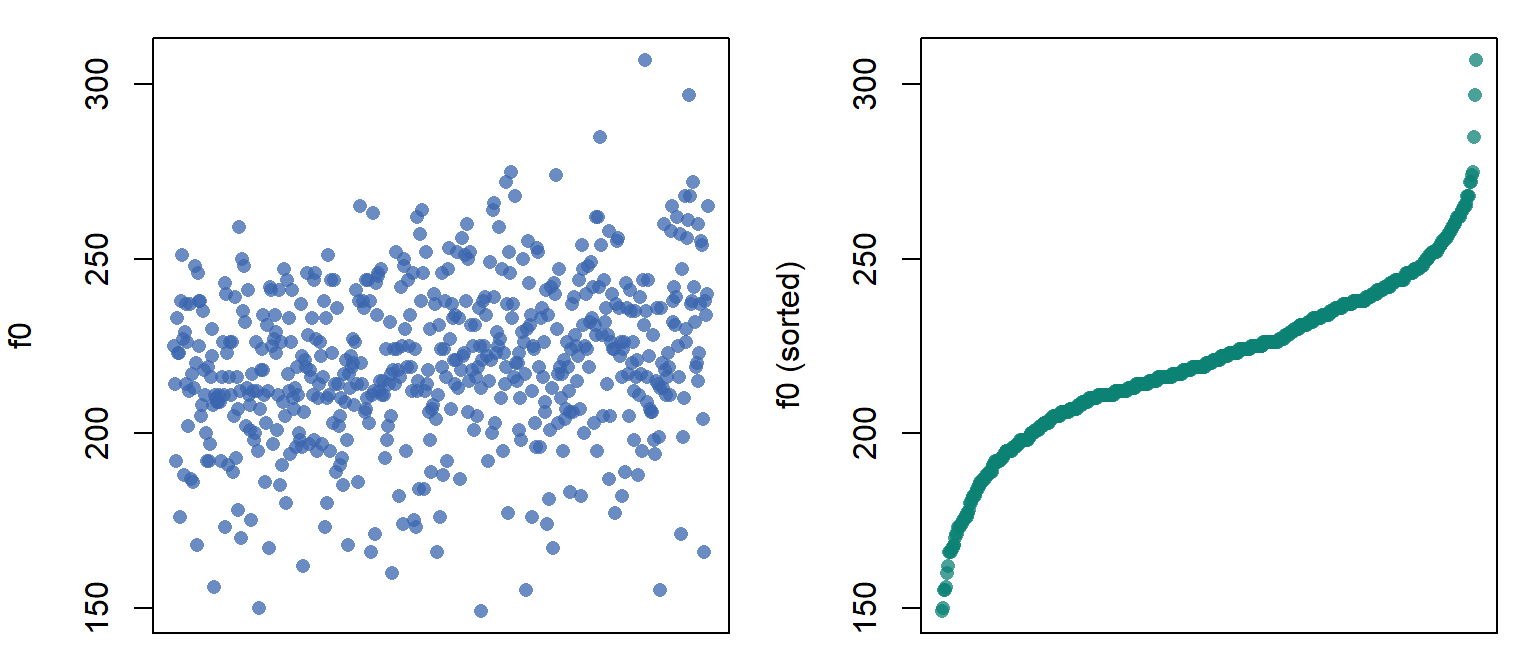
\includegraphics{01_files/figure-latex/initialplot-1.pdf}
\caption{\label{fig:initialplot}(left) Plot of values in the order they appear in the original data. (right) Observations ordered by increasing value.}
\end{figure}

We can look at the distribution of our sample of f0 values in several ways, as seen in Figure \ref{fig:F1-distributioncomparison}. In the top row each point indicates an individual production. Points are jittered along the y axis to make them easier to distinguish so that dense and sparse locations can be compared.

In the middle row we see a box plot of the same data. The edges of the box correspond to the 25\% and 75\% quantiles of the distribution, and the line in the middle of it corresponds to the median. So, the box spans the \emph{interquartile range} of your observations and 50\% of observations are contained in the box. From the edges of the box extend the boxplot `whiskers'. By default, these extend out 1.5 times the interquartile range. These whiskers are simply intended to give you an estimate of the amount of `typical' variation in your sample. Beyond the whiskers we see individual \emph{outliers}, points considered to be substantially different from the rest of the sample. We can see that the boxplot does a good job of summarizing the information in the top row, and provides information related to both average f0 values and to the expected variability in these values.

The bottom row presents what is knows as a \emph{histogram} of the same data. The histogram divides the x axis into a set of discrete sections (`bins'), and gives you the count (or frequency) of observations in each bin. Bins with lots of observations are relatively taller (more \emph{dense}) than bins without many observations in them. As a result, histograms can be used to summarize where observations tend to be. For example, we can see that the bins under the interquartile range have the most observations, and that values further from the mean value become increasingly less frequent.

\begin{figure}

{\centering 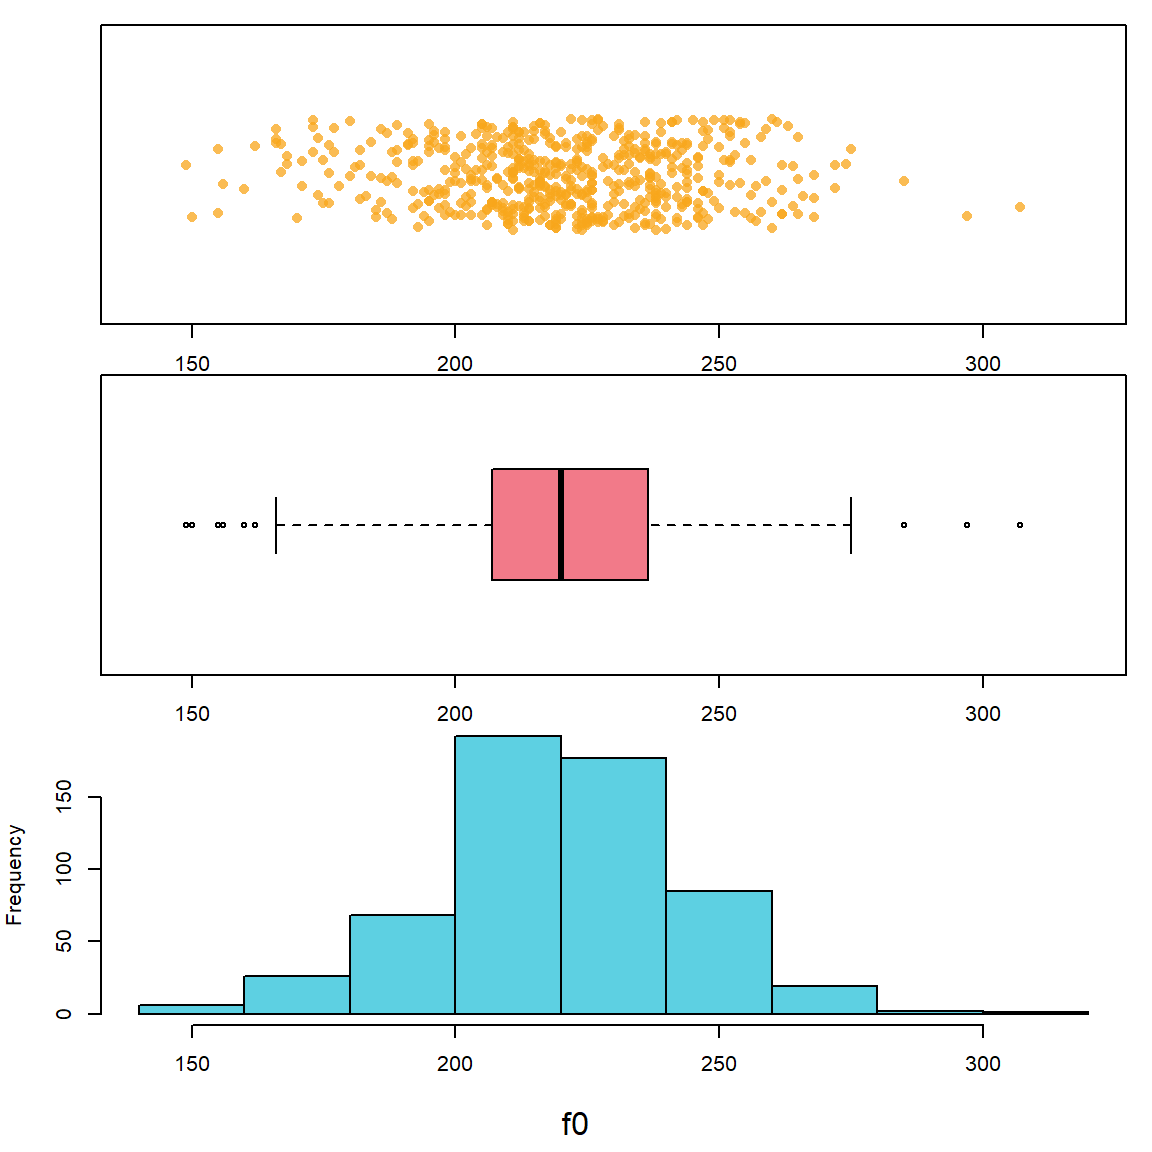
\includegraphics{01_files/figure-latex/F1-distributioncomparison-1} 

}

\caption{Different ways to consider our distribution of f0 values.}\label{fig:F1-distributioncomparison}
\end{figure}

\hypertarget{probability-distributions}{%
\section{Probability Distributions}\label{probability-distributions}}

Histograms are particularly useful to understand because of how they relate to probability distributions. The probability is the number of times an event is expected to occur, out of all the other observed events and outcomes that can occur. This can also be thought of as the \emph{percent} of times an event is expected to occur. For example, the probability that any given day is Monday is 1/7 (14\% of days), while the probability that any given day is a weekday is 2/7 (29\% of days).

By definition, the total probability of all of the possible values in a population is always equal to 1. This is like using 100 to communicate percentages by convention. This is not \emph{correct} or \emph{true}, it is arbitrary just like our base 10 number system. We could make all probabilities add up to 1.37 instead, but why would we want to? Making all probabilities add up to one has many practical advantages and so this convention is actually beneficial for us. As a result of this convention, you know that a probability of 0.5 means something is expected to occur half the time (i.e., on 50\% of trials). For example, suppose we want to know the probability of being an adult female in our sample who produces an f0 under 175 Hz. Finding the probability of observing this event is easy:

\begin{Shaded}
\begin{Highlighting}[]
\CommentTok{\# the evaluation in the parenthesis will return 1 if true, 0 if false}
\CommentTok{\# number of observations the fall below threshold}
\FunctionTok{sum}\NormalTok{ (f0 }\SpecialCharTok{\textless{}} \DecValTok{175}\NormalTok{)  }
\DocumentationTok{\#\# [1] 22}

\CommentTok{\# divided by total number of events}
\FunctionTok{sum}\NormalTok{ (f0 }\SpecialCharTok{\textless{}} \DecValTok{175}\NormalTok{) }\SpecialCharTok{/} \FunctionTok{length}\NormalTok{ (f0)  }
\DocumentationTok{\#\# [1] 0.03819444}

\CommentTok{\# a shortcut to calculate probability, mean = total/length}
\FunctionTok{mean}\NormalTok{ (f0 }\SpecialCharTok{\textless{}} \DecValTok{175}\NormalTok{)}
\DocumentationTok{\#\# [1] 0.03819444}
\end{Highlighting}
\end{Shaded}

The top value is the frequency of the occurrence. This is not so useful because this number can mean very different things given different sample sizes (e.g., 22/23, 22/10000). The middle and bottom values have been divided by the total number of observations. As a result, these now represent a proportion, or probability.

The histogram on the left below shows frequency on the y axis, indicating the total number of observations in each bin. The histogram on the right shows \emph{density} along the y axis. When you see \emph{density} on the y axis, that means that y axis values have been scaled so that the total area of all the rectangles making up the histogram are equal to 1. This has two benefits:

\begin{enumerate}
\def\labelenumi{\arabic{enumi})}
\tightlist
\item
  It lets you compare the distribution of values across different sample sizes.
\item
  It makes the histogram more comparable to a probability distribution.
\end{enumerate}

\begin{figure}
\centering
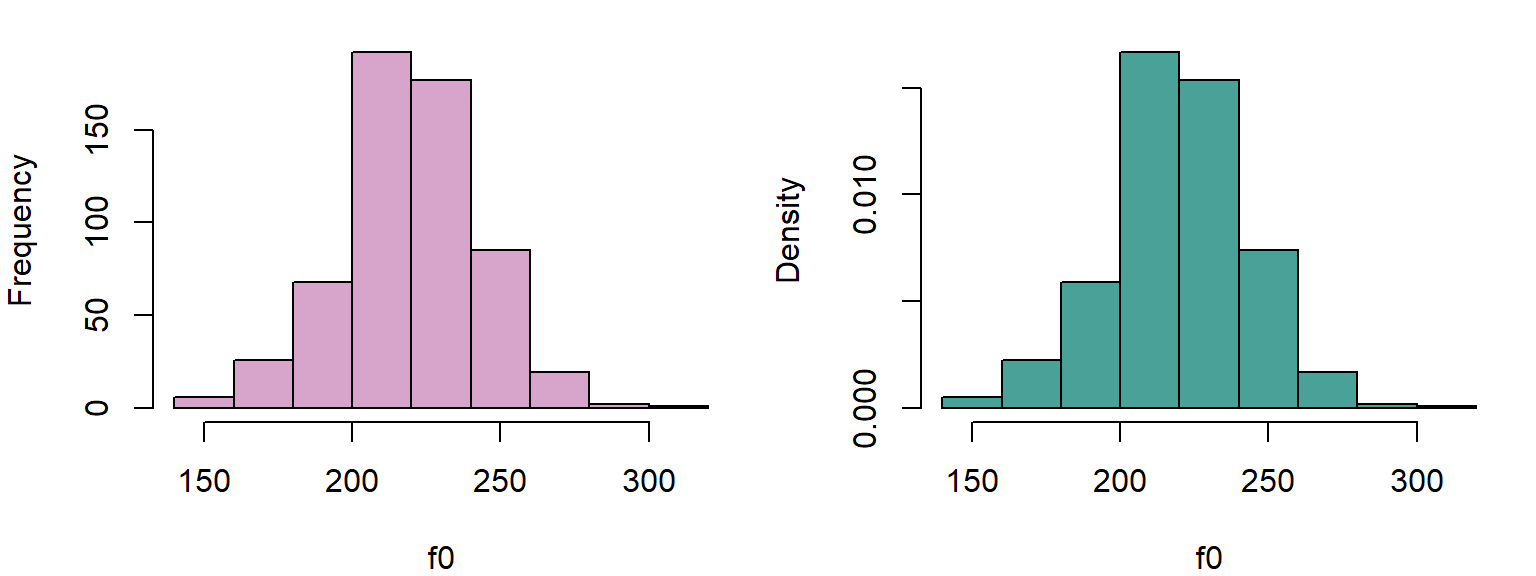
\includegraphics{01_files/figure-latex/F1-twohists1-1.pdf}
\caption{\label{fig:F1-twohists1}(left) A histogram of our f0 data showing counts in each bin. (right) A histogram of our f0 data showing densities.}
\end{figure}

Imagine a circle like in a Venn diagram that contains all possible productions of female f0. This circle has an area of 1 since it contains all possible values in the population. Imagine we spread out this circle along the x axis so that its shape reflected the relative frequencies of different values presents in the population. For example, if some outcomes were 5 times more probable than others, the shape should be 5 times taller there, and so on. If we managed to do this, the height (or `density') of this shape would exactly correspond to a probability distribution like that seen in the right plot above.

The \emph{density} of a histogram (of probability distribution) is just the thickness of the distribution at a certain location along the number line. A higher density in a certain location tells us values in that vicinity are relatively more probable, and differences in density reflect differences in the relative probability of different values.

Below I've repeated the data vector, doubling the counts by including each observation twice. Notice that the y axis in the right panel does not change. This is because increasing the number of observations changes your counts but not the relative frequencies of observations with different values. For instance, increasing the number of coin flips should not change the fact that 50\% will be heads, but it will change the number of heads you observe.

\begin{figure}
\centering
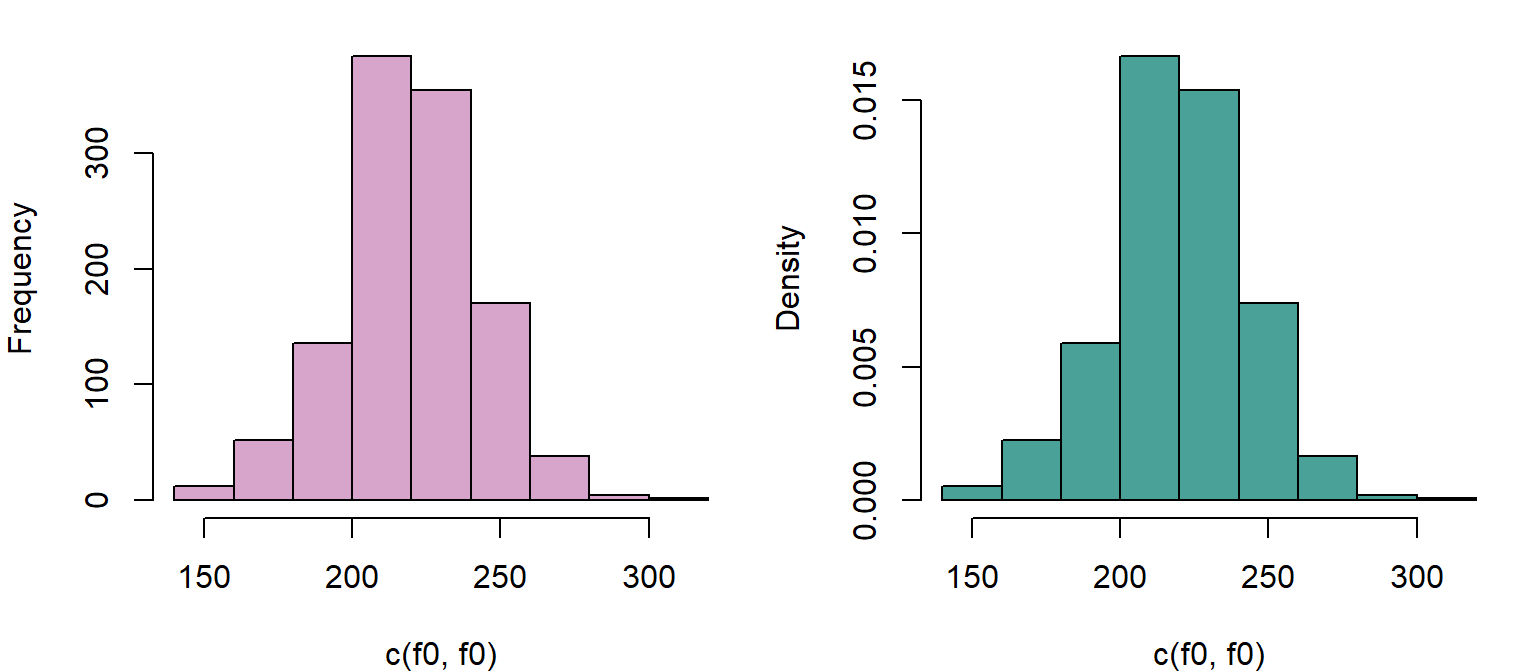
\includegraphics{01_files/figure-latex/F1-twohists2-1.pdf}
\caption{\label{fig:F1-twohists2}The counts have been doubled relative to above.}
\end{figure}

\hypertarget{the-normal-distribution}{%
\subsection{The normal distribution}\label{the-normal-distribution}}

The distribution of many \href{https://www.youtube.com/watch?v=4HpvBZnHOVI}{random variables} (including f0) follows what's called a \href{https://en.wikipedia.org/wiki/Normal_distribution}{normal distribution}, also called a Gaussian distribution. So, if you take a sample of a random variable and arrange observations into bins, they resulting histogram will tend to have the familiar, bell-shaped curve common to normally-distributed data.

The normal distribution has the following important characteristics.

\begin{enumerate}
\def\labelenumi{\arabic{enumi}.}
\item
  The distribution is symmetrical - i.e., producing a higher or lower than average f0 is about equally likely.
\item
  The probability of observing a given value decreases as you get further from the mean (i.e., \emph{average}) value.
\item
  It's easy to work with, very well understood, and naturally arises in basically all domains.
\end{enumerate}

Normal distributions have two parameters. This means they vary from each other in only two ways. Think of parameters like ways that things can be `set' differently from each other. For example, a radio has three parameters: tuner frequency, band (AM/FM), and volume. A toaster may have only one, a single knob determining the degree of toasting required. The more parameters something has, the more complicated it is (an airplane has thousands!).

Luckily, the normal distribution only has two parameters:

\begin{enumerate}
\def\labelenumi{\arabic{enumi}.}
\item
  A mean parameter, \(\mu\), which determines the location of the distribution along the x axis. When the mean changes, the whole shape of the distribution slides along the number line. The mean is the 50\% halfway point of the `mass' of the distribution. If the distribution were an physical object, its mean would be its center of gravity. You would balance the distribution on your fingertip along this point.
\item
  A standard deviation, \(\sigma\), that determines its \emph{spread} along the x axis. When the standard deviation changes the distribution is stretched wide or made very narrow, but stays in place. Since every distribution has an area under the curve equal to one (i.e., they all have the same `volume'), distributions with a small variance must necessarily be very dense.
\end{enumerate}

The parameters of a probability distribution are used to draw its shape, which can be used to make inferences about likely values. Think back to high school math and the function defining the shape of a parabola \(y = ax^2+bx+c\). This function draws a shape based on the settings of its parameters \(a, b\) and \(c\). In the exact same way, the formula defining the density of the normal distribution draws the shape given the settings of its \(\mu\) and \(\sigma\) parameters.

Below, I compare the histogram of f0 values to the density of a normal distribution with a mean equal to our sample mean (\(\mu = 220 Hz\)) and a standard deviation equal to our sample standard deviation (\(\sigma = 23 Hz\)), calculated above. The density was drawn using the \texttt{dnorm} function, which draws a curve representing the shape of a theoretical normal distribution with a given mean and standard deviation.

\begin{figure}
\centering
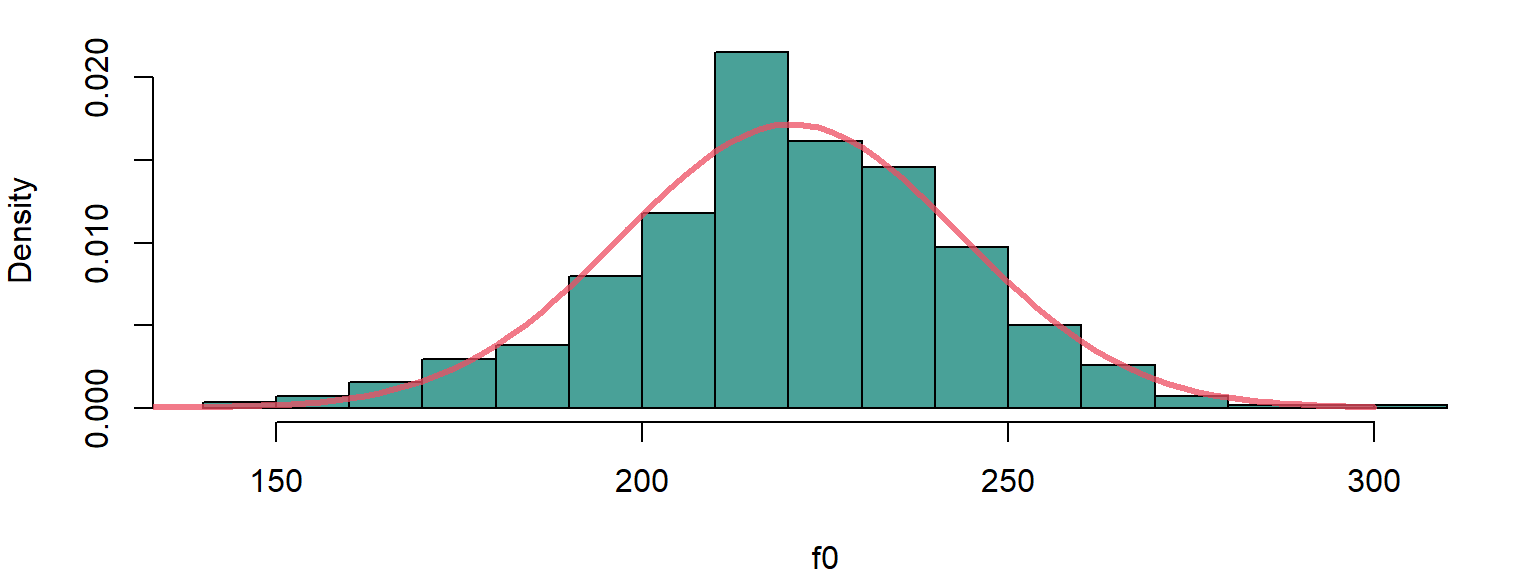
\includegraphics{01_files/figure-latex/theoretical-1.pdf}
\caption{\label{fig:theoretical}A comparison of the data distribution with a theoretical normal distribution.}
\end{figure}

Clearly, there is a very good alignment between our random sample of real-world data and the normal density, which is a theoretical mathematical function. This suggests that we could potentially use the \emph{theoretical} shape of the normal distribution to talk about the characteristics of our observed random sample of data. This would be a bit like using the properties of a parabola to predict the path of a projectile in real life: although the actual path will differ form that of a perfect parabola, there are enough similarities to make the comparison worthwhile.

\hypertarget{referring-to-the-normal-distribution-to-make-inferences}{%
\subsection{Referring to the normal distribution to make inferences}\label{referring-to-the-normal-distribution-to-make-inferences}}

In general, it's impossible to know what the `true' data distribution is, so that \emph{perfect} inference is not possible. As a result, scientists often use theoretical probability distributions to make inferences about real-life populations and observations. Since our f0 measurements follow the `shape' predicted by the theoretical normal distribution, we may be able to use the characteristics of an appropriate normal distribution to make inferences about female f0 (and other variables).

Using a normal distribution to make inferences about your data is like using a mathematical model for spheres to understand the behavior of billiard balls. In reality the balls are not perfect spheres. However, their shapes will be \emph{spherical enough} to allow us to make useful predictions based on the simplified model. In general, it is useful to keep in mind that reality will never exactly conform to our model. This can result in unpredictable errors in our conclusions. In general, the things you don't know you don't know are the things that will cause the most problems. If you know that your model was wrong, you would have fixed it!

Since we expect the distribution of f0 values to have the shape of the normal distribution, we can use the shape of the normal distribution to make inferences about the distribution of f0 values, even the ones we did not observe. For example, we can use the theoretical normal density to estimate the probability of observing a female production with an f0 of under 175 Hz, from among \emph{all} possible values of this random variable (i.e., all observable productions of f0 in this \emph{population}).

We do this by referring to the proportion of values expected to be less 175 Hz in the normal distribution that has the same `shape' as our sample. This can be found by finding the area under the curve of the probability density to the left of that point (the red area below). Since the \emph{total} area is always equal to 1, the area of the red portion below corresponds to a percentage/probability.

Below, I use the function \texttt{pnorm} to find the proportion of values that are expected to be greater/less than 175 Hz. We can do this for the normal density because it is very well understood. Think of how easy it is to calculate the area of a circle of the perimeter of a square. The shape of the normal distribution is only a little more complicated to understand, and the \texttt{pnorm} function helps you make predictions about it.

I use the parameters estimated form our sample to run the \texttt{pnorm}function, as these are our best guesses of the population parameters. As we can see, this value is reasonably close to our empirical probability of 0.038 (3.8\%).

\begin{Shaded}
\begin{Highlighting}[]
\CommentTok{\# Observed probability observing a token with an f0 \textless{} 175 Hz}
\FunctionTok{mean}\NormalTok{ (f0 }\SpecialCharTok{\textless{}} \DecValTok{175}\NormalTok{)}
\DocumentationTok{\#\# [1] 0.03819444}

\CommentTok{\# Theoretical probability of observing a production below 175 Hz}
\FunctionTok{pnorm}\NormalTok{ (}\DecValTok{175}\NormalTok{, }\FunctionTok{mean}\NormalTok{ (f0), }\FunctionTok{sd}\NormalTok{(f0))}
\DocumentationTok{\#\# [1] 0.02527988}

\CommentTok{\# Theoretical probability of observing a production greater than 175 Hz}
\DecValTok{1} \SpecialCharTok{{-}} \FunctionTok{pnorm}\NormalTok{ (}\DecValTok{175}\NormalTok{, }\FunctionTok{mean}\NormalTok{ (f0), }\FunctionTok{sd}\NormalTok{(f0))}
\DocumentationTok{\#\# [1] 0.9747201}
\end{Highlighting}
\end{Shaded}

\begin{figure}
\centering
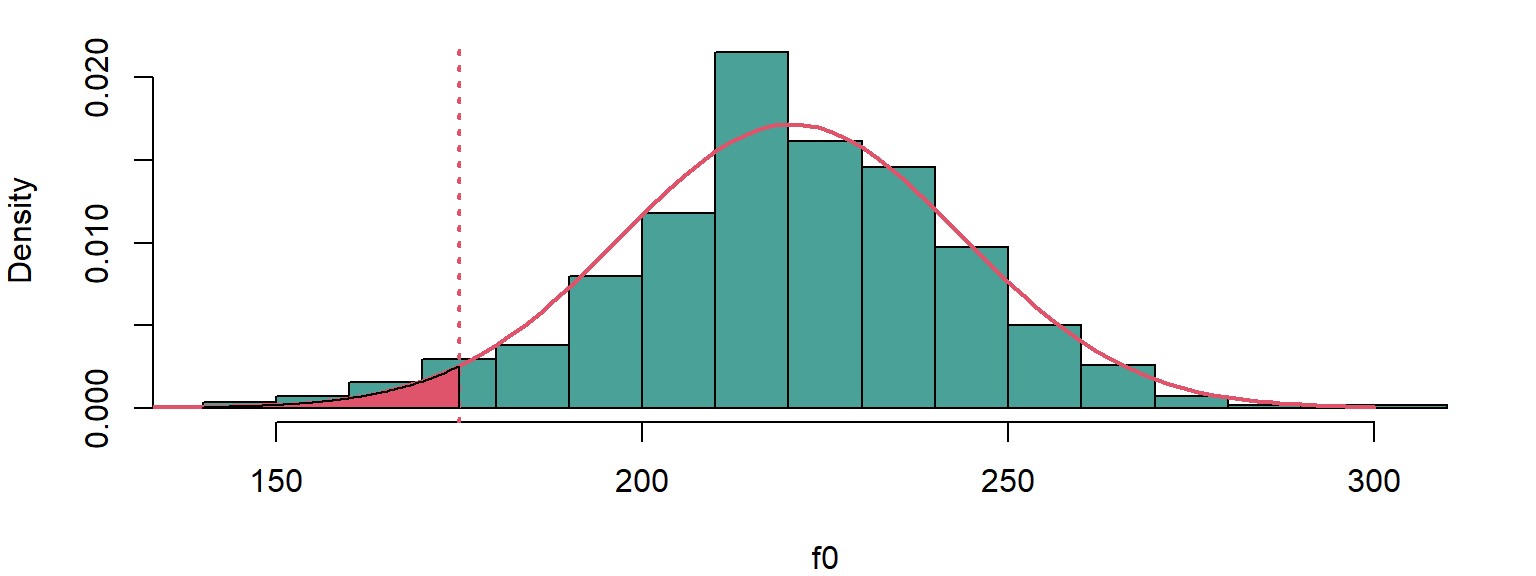
\includegraphics{01_files/figure-latex/F1-prediction-1.pdf}
\caption{\label{fig:F1-prediction}The read area relects the distribution of outcomes that satisfy f0 \textless{} 175 Hz.}
\end{figure}

Imagine you had 1 pound of clay and I asked you to make a shape \textbf{exactly} like the normal density (red curve) above. This shape should be perfectly flat, i.e., it should have a constant depth (like a coin). If you had this shape made of clay used a knife to remove the part left of 175 Hz (the red subsection) and weighed it, it should weigh 2.5\% of a pound. The `area under the curve' of this clay sculpture would just correspond to the amount of clay in a certain area, and in this case we know that only 2.5\% of the clay should be in that section of the shape. So, the area under the curve, the probability, is just the amount of the \emph{stuff} in the density that falls below/above a certain point, or between two points.

We can use the probabilities to compare our predicted and expected observations. Since we had 576 observations and there was a probability of 0.025 of observing tokens with an f0 below 175 Hz, we expect about 14 tokens (\(576 \times 0.025\)) to have an f0 lower than 175 Hz. Instead, we have 22 such observations indicating that our actual data has more extreme values than our theoretical distribution.

\begin{Shaded}
\begin{Highlighting}[]
\CommentTok{\# probability of observing a production with an f0 under 175 Hz}
\NormalTok{probability }\OtherTok{=} \FunctionTok{pnorm}\NormalTok{ (}\DecValTok{175}\NormalTok{, }\FunctionTok{mean}\NormalTok{ (f0), }\FunctionTok{sd}\NormalTok{(f0)) }

\CommentTok{\# expected count}
\FunctionTok{length}\NormalTok{ (f0) }\SpecialCharTok{*}\NormalTok{ probability}
\DocumentationTok{\#\# [1] 14.56121}

\CommentTok{\# actual count}
\FunctionTok{sum}\NormalTok{ (f0 }\SpecialCharTok{\textless{}} \DecValTok{175}\NormalTok{)}
\DocumentationTok{\#\# [1] 22}
\end{Highlighting}
\end{Shaded}

\hypertarget{probabilities-of-events-and-likelihoods-of-parameters}{%
\section{Probabilities of events and likelihoods of parameters}\label{probabilities-of-events-and-likelihoods-of-parameters}}

We're going to switch from talking about \emph{probabilities} to talking about \emph{likelihoods}. A probability is the odds of observing some data/event/outcome, given some parameter(s). A likelihood places odds on different \emph{parameter} values given some observed data. These concepts are basically the inverse of each other. For example, you could say ``how probable is it that a random person from San Francisco will be over 6 feet tall?''. In contrast, you could ask ``how likely is it that the average height of people from San Francisco is 6 feet?''.

The \emph{likelihood function} is a curve showing the relative likelihoods of different parameter values, given a fixed set of data. The likelihood function tells you what values are \emph{believable} given your data. If a value is very unlikely, that means that it is not supported by your data. In other words, unlikely parameter estimates represent conclusions that your data is rejecting as not viable. Every parameter for every probability distribution has a likelihood function, given some data. Here, we're only going to discuss the likelihood of the normal mean parameter, \(\mu\), in detail.

Here are three useful properties of the likelihood functions of \(\mu\), the mean parameter of the normal distribution:

\begin{enumerate}
\def\labelenumi{\arabic{enumi}.}
\item
  The likelihood function of \(\mu\) will tend to be a normal distribution.
\item
  The mean (and peak) of the likelihood function of \(\mu\) given some sample \(x\) is equal to the arithmetic mean of the sample (\texttt{mean(x)}).
\item
  The standard deviation of the likelihood of \(\mu\) is equal to the standard deviation of the data (\texttt{sd(x)}), divided by the square root of N (the sample size).
\end{enumerate}

The first point tells us that we can use the normal distribution to make inferences about likely, and unlikely values for means, given some data.

The second point says that if you are wondering what the best (most likely) estimate of the population mean is given your sample, the answer is the arithmetic mean of your sample (\(\bar{x}\)).

The third point means that the likelihood function for \(\mu\) will tend to be \emph{much} narrower than the distribution of our original data. This is because a mean based on, for example, 50 samples will contain many positive and negative deviations from the average that will tend to cancel out. As a result, the more data you have the more \emph{precise} your estimates are, and the less \emph{uncertainty} is associated with any estimate. This is why scientists focus so much on sample size when they conduct statistical analyses.

Figure \ref{fig:F1-likelihood1} shows the likelihood function for \(\mu\) based on the first 10 observations of our f0 vector (indicated by the blue points at the bottom of the plot). I chose this small sample just to make this example clearer. Notice that the most likely mean values of \(\mu\) for these points like over the bulk of the sampled values. The vertical dotted lines show three possible mean values that will be highlighted in this discussion.

The likelihood of any parameter estimate (e.g., \(\mu\) = 175 Hz in the right panel of Figure \ref{fig:F1-likelihood1}) is equal to the product of the density of each observation in the sample, if we assume that the estimate were true. This is actually deceptively simple. For example, to calculate the likelihood that \(\mu=175\), we:

\begin{enumerate}
\def\labelenumi{\arabic{enumi})}
\item
  Assume that the data is generated by a normal distribution with a \(\mu\) equal to 175 Hz, and \(\sigma\) equal to the sample standard deviation of 23 Hz.
\item
  Find the the height of the curve of the probability distribution (the density) over each point (indicated by the vertical lines in the right panel below).
\item
  The likelihood is the product of all of these densities (heights). In practice, often the logarithms of the individual probabilities are added together, yielding the \emph{log-likelihood}. This is because multiplying together too many fractions can lead to numbers so small computers have a hard time representing them, and adding logarithms is equivalent to multiplying the original values.
\end{enumerate}

Imagine I follow the steps above for each position along the x axis, recording the likelihood values I calculate. I then plot the product of the densities for each corresponding x value. If I do this I have just plotted a likelihood function for \(\mu\) given our data, and the result would be a curve identical to that of the left panel in \ref{fig:F1-likelihood1}.

~
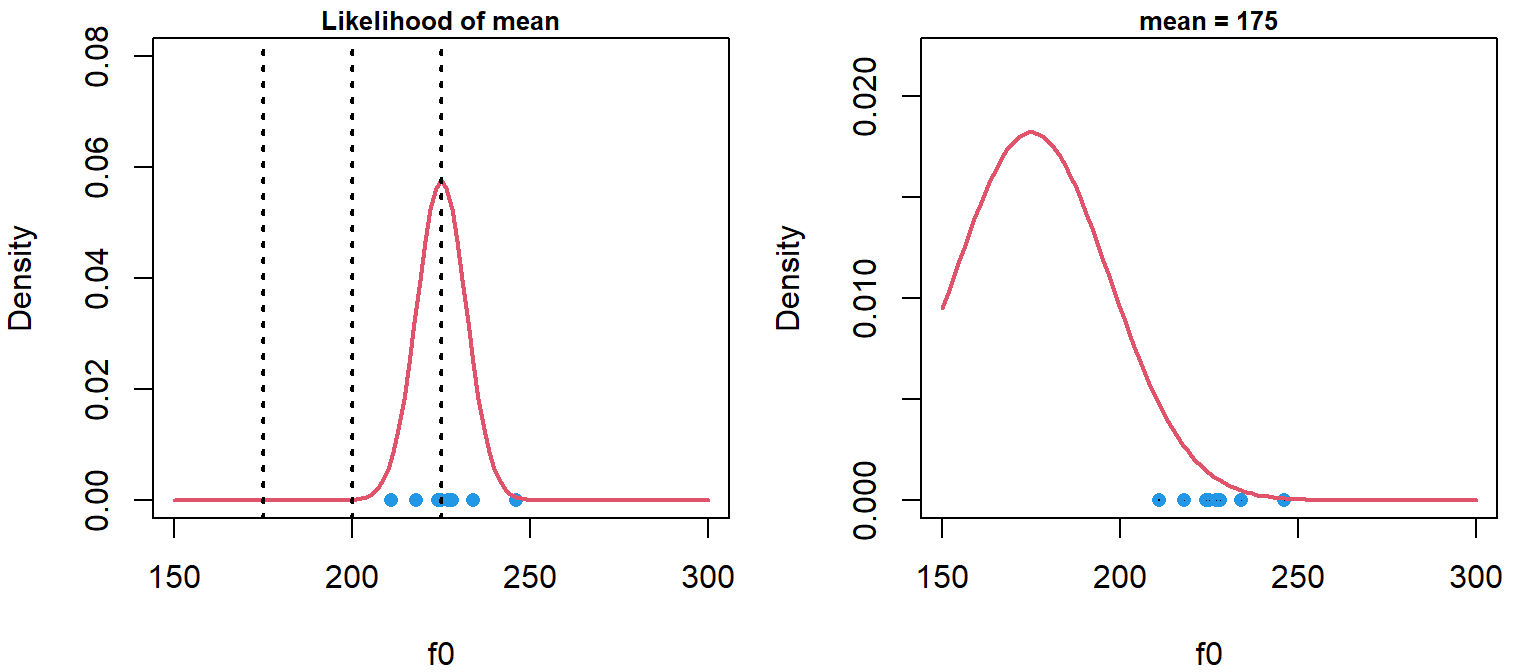
\includegraphics{01_files/figure-latex/F1-likelihood1-1.pdf}
~

In the right panel in Figure \ref{fig:F1-likelihood1} we see that a normal distribution with a \(\mu\) of 175 Hz is very unlikely to generate this data. Many points are extremely improbable and have densities close to zero. As a result, the product of these values (the heights of the lines) will be a very small number. This is reflected in the extremely small values in the likelihood function at 175 Hz in the left panel above.

In the left panel in Figure \ref{fig:F1-likelihood2}, we see that a normal distribution with a \(\mu\) of 200 Hz is more likely to generate this data, and the probability distribution is clearly a much better fit. However a distribution with a mean of 200 Hz is still not very likely to have generated this data.

Finally, in the right panel below we see the the maximum likelihood estimate for this sample of 225 Hz, the value representing the peak of the likelihood function (in the left panel above). When we say that 225 Hz is the most likely mean for this data, we are saying that this data is probably generated by a normal distribution centered at 225 Hz, relative to the alternatives.

~
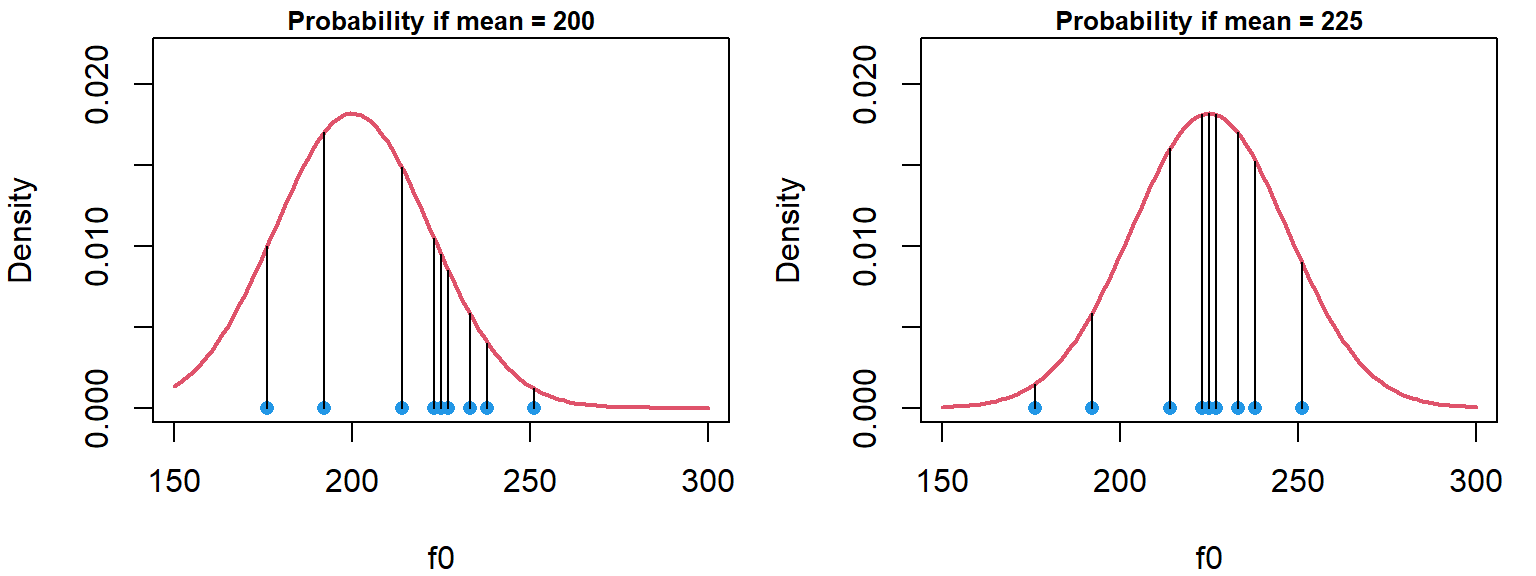
\includegraphics{01_files/figure-latex/F1-likelihood2-1.pdf}
~

\hypertarget{making-inferences-using-likelihoods}{%
\subsection{Making inferences using likelihoods}\label{making-inferences-using-likelihoods}}

Previously, we discussed using the normal distribution to make inferences about the probable values of random variables. When variables are normally distributed we can use the theoretical normal distribution and functions such as \texttt{pnorm} to answer questions about values we expect, and don't expect, to see. We can take this same approach to make inferences about \emph{parameters} when their likelihood functions follow a normal distribution.

It helps to understand this if we start thinking about our parameters as random variables themselves. Think of the average height of the people in a large city. You can go out and sample 100 individual people, and each one of those samples is an observation from a random variables. You can find the mean of your sample, arriving at a single estimate of the population mean. Now imagine that 50 people went out in the same city and each sampled 100 random people. There is no chance that every single of those 50 people would find identical means across all of their samples. Instead, there will be a distribution of sample means, in the same way there is a distribution of the original data used to calculate the means.

We know that our f0 data is approximately normally distributed. As a result, we know the following information:

\begin{enumerate}
\def\labelenumi{\arabic{enumi})}
\item
  The likelihood function of our sample mean parameter follows a normal distribution.
\item
  The mean of this distribution is equal to the sample mean, the mean of our observations.
\item
  The standard deviation of this distribution is equal to the standard deviation if the samples, divided by the square root of the sample size (\texttt{sqrt(576)=24}).
\end{enumerate}

We can calculate these values and use them to draw the curve representing the likelihood function given our data and model structure. You may be thinking, what model? It may seem too simple to be a model, but by assuming that our data can be understood as coming from a normal distribution with some given \(\mu\) and \(\sigma\), we have already created a simple model for our data. I'll return to this below.

We can also use the \texttt{qnorm} function to calculate quantiles for our likelihood, presented below. Vertical lines have been added at the 2.5\% and 97.5\% quantiles of the distribution. These vertical lines enclose 95\% of the likelihood density, and so represent the range of values representing the 95\% most likely values of \(\mu\). I chose an interval enclosing 95\% of the likelihood because this is used by convention. This is a commonly-used interval but otherwise has no special significance.

\begin{Shaded}
\begin{Highlighting}[]
\CommentTok{\# sample mean}
\FunctionTok{mean}\NormalTok{ (f0)   }
\DocumentationTok{\#\# [1] 220.401}

\CommentTok{\# sample standard deviation}
\FunctionTok{sd}\NormalTok{ (f0)     }
\DocumentationTok{\#\# [1] 23.22069}

\CommentTok{\# sample size}
\FunctionTok{length}\NormalTok{ (f0)  }
\DocumentationTok{\#\# [1] 576}

\CommentTok{\# the standard deviation of the likelihood function}
\FunctionTok{sd}\NormalTok{ (f0) }\SpecialCharTok{/} \FunctionTok{sqrt}\NormalTok{ ( }\FunctionTok{length}\NormalTok{ (f0) ) }
\DocumentationTok{\#\# [1] 0.9675289}

\CommentTok{\# the 2.5\% and 97.5\% quantiles of the likelihood function}
\FunctionTok{qnorm}\NormalTok{ (}\FunctionTok{c}\NormalTok{(}\FloatTok{0.025}\NormalTok{, }\FloatTok{0.975}\NormalTok{), }\FunctionTok{mean}\NormalTok{ (f0), }\FunctionTok{sd}\NormalTok{ (f0) }\SpecialCharTok{/} \FunctionTok{sqrt}\NormalTok{ (}\FunctionTok{length}\NormalTok{ (f0) ) )}
\DocumentationTok{\#\# [1] 218.5047 222.2974}
\end{Highlighting}
\end{Shaded}

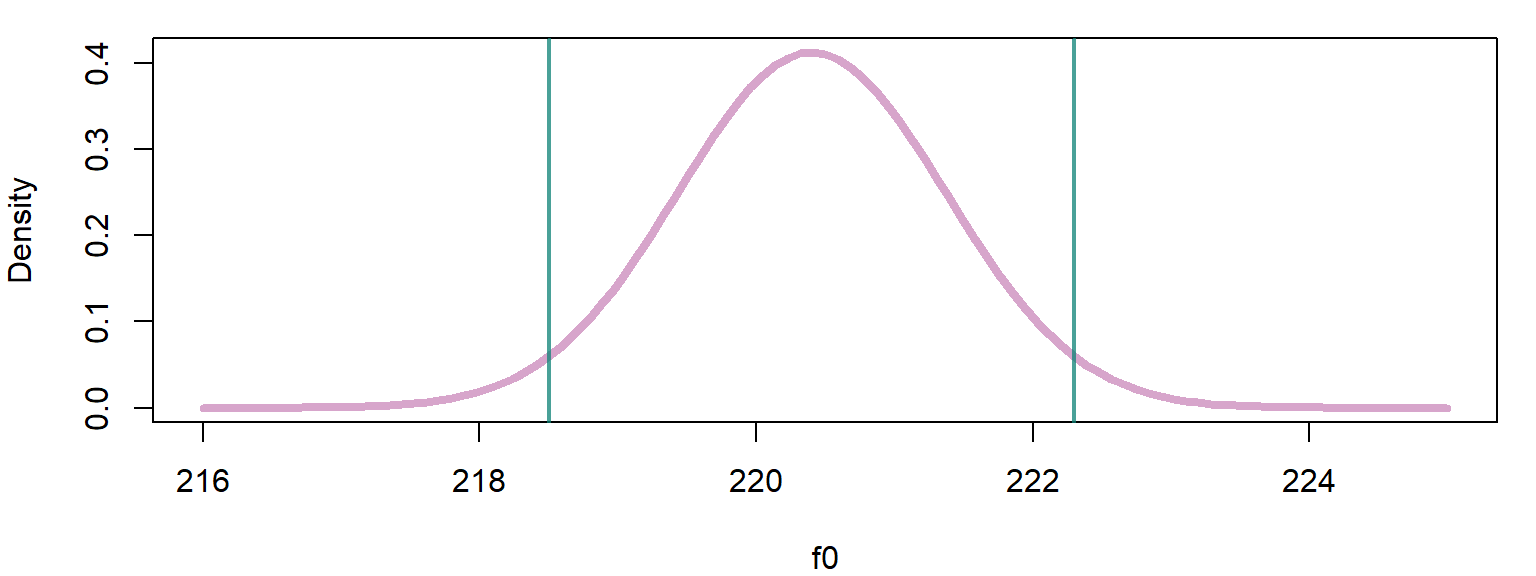
\includegraphics{01_files/figure-latex/F1-likelihood-1.pdf}
~

The likelihood tells you about the most believable/credible parameter values, given your model and data. Given the information presented in the figure above, we may conclude that the most likely parameter values fall between (around) 218 and 222 Hz. This means that it is reasonable that the true population mean might be 221 Hz, as this value is very likely given our sample. Basically, maybe our sample mean is wrong and arose by accident, and 221 Hz is the true population \(\mu\). This outcome is compatible with our data.

However, a value of 216 Hz is extremely \emph{unlikely} to fit our data. It is just too far from our sample mean relative to the amount of variation in our sample. This is like if you measured the heights of 100 women in a small town (pop. 1500) and found the average was 5'4``. You might accept that the actual population average is 5'5'', but may find it difficult to accept that it was actually 6'0". It would mean you happened to measure all of the shortest women in the town, an extremely unlikely event.

So, since we think that 216 Hz is not a plausible mean f0 given our sample, this also means that it is very unlikely that the real \(\mu\) is 216 Hz. This is because a distribution centered at 216 would be extremely unlikely to generate a sample mean of 220 Hz. Using this approach, we can rule out implausible values of \(\mu\) based on the characteristics of our data.

At this point we can offer conventional responses to the research questions posed at the start of the Chapter:

Q1) What is the average f0 of the whole \emph{population} likely to be?

A1) The most likely value for the population mean is our sample mean, 220.4 Hz.

Q2) Can we set bounds on likely mean f0 values based on the data we collected?

A2) Yes, there is a 95\% probability that the population mean is between 218.5 222.3 Hz, given our data and model structure.

Traditional approaches to statistics (sometimes generally referred to as `frequentist') estimate parameters by trying to find the most likely values for parameters (i.e., `maximum likelihood estimation'). They do this by referring to the theoretical likelihood functions such as what we plotted above. Although this works very well for simple data, it is difficult if not impossible for some of the more complicated datasets that often arise for even the simplest research questions in linguistics.

\hypertarget{bayesian-models}{%
\section{Bayesian models}\label{bayesian-models}}

In this class we are going to learn about \emph{multilevel Bayesian models}. These models have many advantages over `traditional' approaches. They provide researchers with more information, are more robust, and at \textbf{worst}, they are as good as traditional models. I may sound biased, but the main reason for all of these advantages is that traditional models were developed over 100 years ago. On the other hand, mathematical and technological advances have only made Bayesian multilevel models possible in the last 10+ years. It's only reasonable that the newer approaches should offer some advantages over methods developed before calculators existed.

Here, I am going to address what is meant by two aspects of the term `Bayesian multilevel models': `Bayesian' and `models'.

\hypertarget{what-are-regression-models}{%
\subsection{What are regression models?}\label{what-are-regression-models}}

Before beginning this section I just want to say that its ok if a lot of this section doesn't makes sense right now. It will make more sense once you start to actually build models and it becomes less hypothetical and more practical. I will use the terms and concepts described here in later chapters, but I will re-explain it each time. If you think that a model in a later section is not explained in as much detail as you would like, look at this section again!

I have been referring somewhat obliquely to `models' without really explaining what I mean by this. It's difficult to offer a precise definition because the term is so broad, but `regression' modeling can be thought of as trying to understand variation the mean parameter (\(\mu\)) of a normal distributions. Actually, you can use many other probability distributions, but for now we will focus on models based on the normal distribution.

Basically it goes like this:

\begin{itemize}
\item
  you have a variable you are interested in, \(y\), which is is a vector containing N observations. We can refer to any one of these observations like this \(y_{[i]}\) for the \(i^{th}\) observation. In our case this is a vector of 576 f0 values (\texttt{f0{[}1:576{]}}). Although its not necessary, I am going to put the index variables associated with trial number (\(i\)) in brackets like this \(y_{[i]}\). This is just to make it easier to identify, and to highlight the similarity to vectors (e.g., \texttt{f0{[}i{]}}).
\item
  you assume that your data is well described by a normal probability distribution. This is a mathematical function (\(\mathcal{N}(\mu,\sigma)\)) that describes what is and is not probable based on two parameters.
\item
  the mean of this distribution is either fixed, or varies in a systematic manner.
\item
  the variation in the mean of this distribution can be understood using some other variables.
\end{itemize}

We can write this model more formally like this:

\[
y_{[i]} \sim \mathcal{N}(\mu,\sigma)
\label{eq:1}
\]

This says that we expect that the tokens of the variable we are interested in is distributed according to (\(\sim\)) a normal distribution with those parameters.

Notice hat \(y\) gets a subscript while \(\mu\) and \(\sigma\) do not. This is because for right now, those parameters are fixed for all observations, while the value of \(y\) changes for each observation based on the \(i\) subscript. For example, below I set \(i=2\) and use this index variable to show the second element of the data vector, i.e.~\(f0_{[i=2]}=214\).

\begin{verbatim}
f0[1:6]
i = 2
f0[i]
\end{verbatim}

Equation \eqref{eq:1} just formalizes the fact that we think the \emph{shape} of our data will be like that of a normal distribution with a mean equal to \(\mu\) and a standard deviation equal to \(\sigma\).

When you see this, \(\mathcal{N}(\mu,\sigma)\), just picture in your mind the shape of a normal distribution, like if you see this \(y=x^2\) you may imagine a parabola. \(\mathcal{N}(\mu,\sigma)\) Really just represents that shape of the normal distribution, and the associated expectation about more and less probable outcomes.

The above relationship can also be presented like this:

\[
y_{[i]} = \mu + \mathcal{N}(0,\sigma)
\label{eq:2}
\]

Notice that we got rid of the \(\sim\) symbol, moved \(\mu\) out of the distribution function (\(\mathcal{N}()\)), and that the mean of the distribution function is now 0. This breaks up our variable into two components:

\begin{enumerate}
\def\labelenumi{\arabic{enumi})}
\item
  A systematic component, \(\mu\), that contributes the same value to all instances of a variable.
\item
  A random component, \(\mathcal{N}(0,\sigma)\), that causes unpredictable variation around \(\mu\).
\end{enumerate}

In terms of our data, I might express the distribution in either of the following ways:

\[
f0_{[i]} = \mathcal{N}(220.4,23.2)
\label{eq:3}
\]

\[
f0_{[i]} = 220.4 + \mathcal{N}(0,23.2)
\label{eq:4}
\]

The distribution on the left below is the original data, centered at 220.4 Hz and with a standard deviation of 23.2 Hz. On the right, the mean has been subtracted from each value. The sample now represents random variation around the sample mean, variation that our model can't explain. From the perspective of our model, this is \emph{noise}, or \emph{error}. This doesn't mean that it's unexplainable, it only means that we've structured our model in a way that doesn't let us explain it. Right now our model basically says ``I know the mean is 220.4 Hz but the rest of the variation in values of f0 is random''.

\begin{figure}
\centering
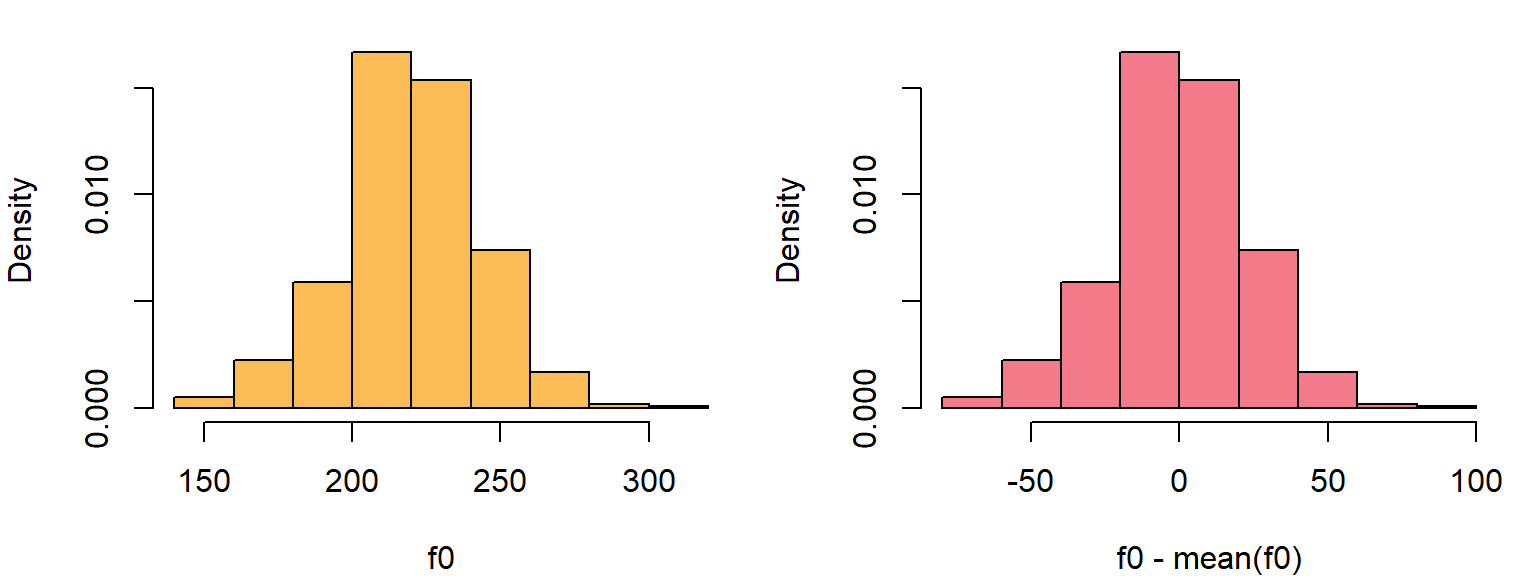
\includegraphics{01_files/figure-latex/F1-errorhist-1.pdf}
\caption{\label{fig:F1-errorhist}(left) Histogram of data. (right) Histogram of centered data, basically the error distribution.}
\end{figure}

In regression models, we can decompose systematic variation in \(\mu\) into component parts, based on some predictor variables, \(\mathrm{x}\). These predictor variables co-vary (vary with) our \(y\) variable, and we think help explain the variation in \(y\).

Below, I am saying that I think \(\mu\) is actually equal to some combination of \(\mathrm{x}_{1}\) \(\mathrm{x}_{2}\) and \(\mathrm{x}_{3}\). For example, I could think that f0 is affected by the speaker age (\(\mathrm{x}_{1}\)) and gender of the speaker (\(\mathrm{x}_{2}\)), and vowel category (\(\mathrm{x}_{3}\)) of the production.

\[
\mu = \mathrm{x}_{1} + \mathrm{x}_{2} + \mathrm{x}_{3}
\label{eq:5}
\]

The values of the predictor variables will vary from trial to trial, and are not fixed. Often the whole point of running an experiment is to predict differences in observations based on differing predictor values! So obviously, \(\mu\) will need to vary from trial to trial. That means that the equation above should actually include \(i\) subscripts indicating that the equation refers to the value of the predictors and expected mean, \emph{for that trial} rather than overall.

\[
\mu_{[i]} = \mathrm{x}_{1[i]} + \mathrm{x}_{2[i]} + \mathrm{x}_{3[i]} \label{eq:5}
\]

Actually, the mean is very unlikely to just be an equal combination of the predictors, so that a \emph{weighting} of the predictors will be necessary. We can use the symbol \(\alpha\) for these weights. For example, maybe \(\mathrm{x}_{1}\) is twice as important as the other two predictors and so \(\alpha_1\) is 2, while \(\alpha_2\) and \(\alpha_3\) are 1.

\[
\mu_{[i]} = \alpha_1*\mathrm{x}_{1[i]} + \alpha_2*\mathrm{x}_{2[i]} + \alpha_3*\mathrm{x}_{3[i]}  
\label{eq:6}
\]

Note that the weight terms (\(\alpha\)) do not get an \(i\) subscript. This is because they do not change from trial to trial. The \emph{values} of the predictors change from trial to trial, but the way that these are combined does not, they are a stable property of the model.

Decomposition of \(\mu\) into sub-components makes our model something more like:

\[
y_{[i]} = \mu_{[i]} + \mathcal{N}(0,\sigma)  
\label{eq:7}
\]

\[
y_{[i]} =  (\alpha_1*\mathrm{x}_{1[i]} + \alpha_2*\mathrm{x}_{2[i]} + \alpha_3*\mathrm{x}_{3[i]} ) + \mathcal{N}(0,\sigma)  
\label{eq:8}
\]

Often, \(\varepsilon\) is used to represent the random component, as in:

\[
y_{[i]} = \alpha_1*\mathrm{x}_{1[i]} + \alpha_2*\mathrm{x}_{2[i]} + \alpha_3*\mathrm{x}_{3[i]}+ \varepsilon_{[i]}
\label{eq:9}
\]

Notice that the error term \emph{does} get a, \(i\) subscript, as in \(\varepsilon_{[i]}\). That is because the exact value of the error changes from trial to trial, even of the general characteristics of the error (i.e., \(\mathcal{N}(0,\sigma)\)) do not.

When expressed in this manner, this is now a `regression equation' or a `regression model'. `Fitting' a regression model basically consists of trying to guess the most likely values of \(\alpha_1\), \(\alpha_2\), and \(\alpha_3\) given our data.

Notice that the above formulation means that regression models do not require that our \emph{data} be normally distributed, but only that the \emph{random variation} in our data (\(\varepsilon\)) be normally distributed. For example, in the left panel below I plot the distribution of f0 from among the entire Hillenbrand et al.~data, including boys, girls, men and women. The data is not normally distributed, however, we can still use a regression based on normally-distributed data to model this as long as we expect that:

\begin{enumerate}
\def\labelenumi{\arabic{enumi})}
\item
  There is systematic variation in the \(\mu_{[i]}\) of f0 across different groups, speakers, conditions, etc.
\item
  The \emph{random variation} around these predicted values of \(\mu_{[i]}\) more or less follows a normal distribution.
\end{enumerate}

In the right panel I plot the individual densities for different speaker classes. We see that although the data is not normally distributed, the within-group variation is. This suggests a regression model is appropriate for this data.

\begin{figure}
\centering
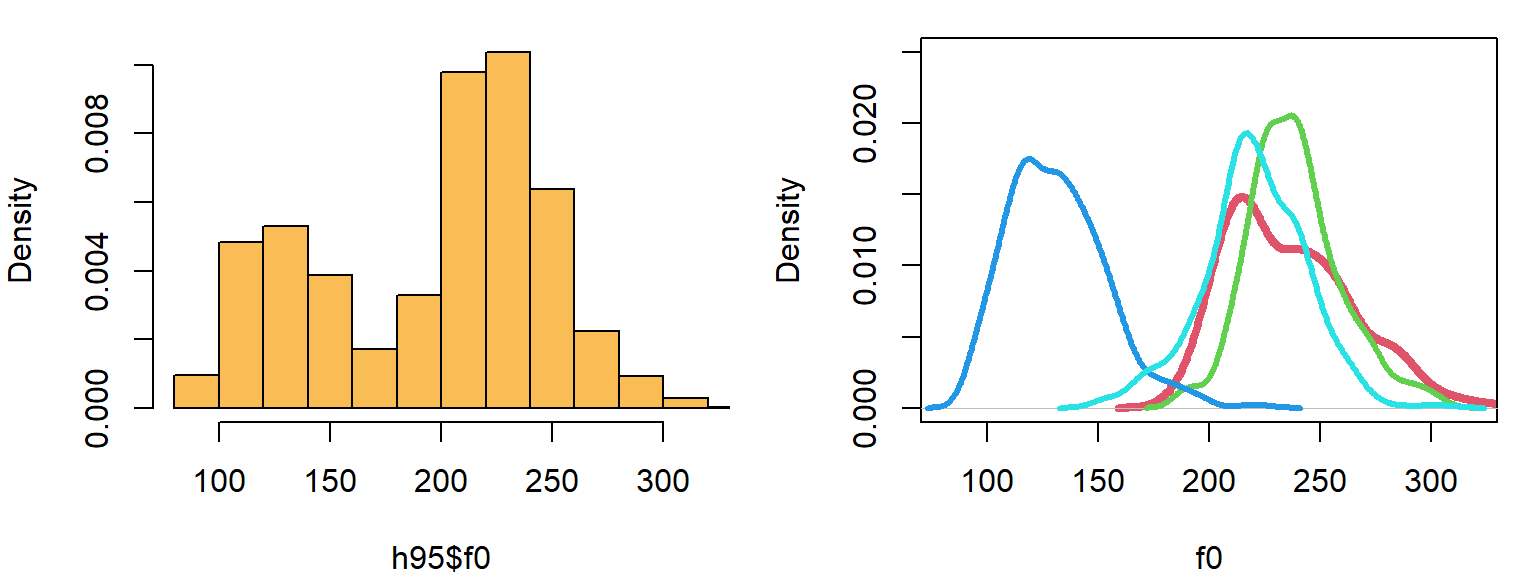
\includegraphics{01_files/figure-latex/F1-allf0s-1.pdf}
\caption{\label{fig:F1-allf0s}(left) Distribution of f0 across all speakers. (right) Densities of distributions of f0 for different speaker classes: boys (red), girls (green), men (blue) and women (cyan).}
\end{figure}

\hypertarget{whats-bayesian-about-these-models}{%
\subsection{What's `Bayesian' about these models?}\label{whats-bayesian-about-these-models}}

The major difference between Bayesian and traditional models is that Bayesian models rely on \emph{posterior distributions} rather than likelihood functions. I am going to define some terms:

\begin{itemize}
\item
  prior probability distribution: the distribution of possible/believable parameter values \textbf{prior} to the \emph{current} experiment. This \emph{a priori} expectation can come from world knowledge, previous experiments, or some combination of the two. Before ytou measure the height of adults in San Francisco, you know the average is not 4 feet and it is not 7 feet.
\item
  the likelihood: this is the distribution of possible/credible parameter values given the \textbf{current} data and probability model, and nothing else. After you go out and measure the heights of some adults, you have more and less believable conclusions based on your data.
\item
  posterior probability distribution: the distribution of possible/believable parameter values you have \textbf{after} your current experiment. You get this by combining the prior distribution and the likelihood. Maybe you went in there thinking people in San Francisco were relatively short. After sampling many tall people you update your beliefs somewhat, adjusting these based on the new information.
\end{itemize}

So, more traditional models focus exclusively on how likely different conclusions are given only your data, while Bayesian models combine notions of likelihood with prior beliefs. The use of prior probabilities is often said to make Bayesian models `subjective' but its not really a big deal. First, every model involves arbitrary decisions which can substantially affect our results. Second, a researcher will always use common sense to interpret a model. For example, before collecting my sample I can say that I expect my female average f0 to be 200 Hz or so, but think its reasonable to expect anything from 100 to 300 Hz. Based on everything we know about human speech, even these bounds are too wide and anything outside this would suggest something is very wrong. So, even if I did not specifically assign prior probabilities to results, I would still use my expectations to `screen' my results, and be very wary of anything that did not meet my expectations.

A Bayesian model simply requires that you build your expectations into your model. It formalizes it, makes it definable and replicable. Also, being `objective' does not quite make sense in many cases. Is it really being `objective' to ignore common sense and act as if a mean f0 of 250 is exactly as likely a priori as one of 20,000 Hz? In any case, in practice the prior probabilities hardly have any effect on our outcomes, and employing them allows our Bayesian models to be extremely flexible and robust.

\hypertarget{posterior-distributions}{%
\section{Posterior distributions}\label{posterior-distributions}}

The combination of probability distributions is straightforward conceptually: you just multiply the values of the distributions at each x-axis location, and the result is the new curve. In the figure below several sets of probability distributions are combined, showing the effects of variations in priors and likelihoods. In each plot, the posterior density has been scaled so that it is the same height as the likelihood. This is only to make the figures interpretable but does not affect any of the points I make below.

In the top-left panel, I plot the likelihood function for \(\mu\) given a sample of size 5 with a mean of 220 Hz. This is combined with a relatively weak but very different prior: the standard deviation is the same as our f0 data, however the mean is much higher (250 Hz). The curve indicating the posterior is nothing more than the product of the prior and the likelihood at each x axis location. We can see that even with only 5 data points the likelihood already dominates the posterior, though the prior distribution is exerting a pull.

In the top-right panel, the posterior is almost identical to the likelihood. The likelihood represents a sample of size 100, which is actually a tiny sample in experimental linguistics work where you may have 200+ samples from each of 50+ subjects and 10,000 observations overall. As you might imagine, when the sample size is that large the prior exerts almost no influence on results.

In the bottom-left panel we see the same likelihood as in the top-left panel based on only 5 observations. In this case the prior the prior has been made very narrow and therefore dominates the estimate. Consider a situation where we actually have really good reasons to think that the mean is 250 Hz. If we really \emph{know} this, why would we accept and estimate of 220 Hz based on only 5 samples? In this case, the posterior distribution is basically saying: your estimate is great, but come back when you have more evidence and I might believe you.

In the bottom-right panel we see a situation where the likelihood and the prior are equal. Since they are about equally believable the posterior represents a perfect compromise between new and prior knowledge, forming a distribution exactly between the prior and the likelihood.

\begin{figure}
\centering
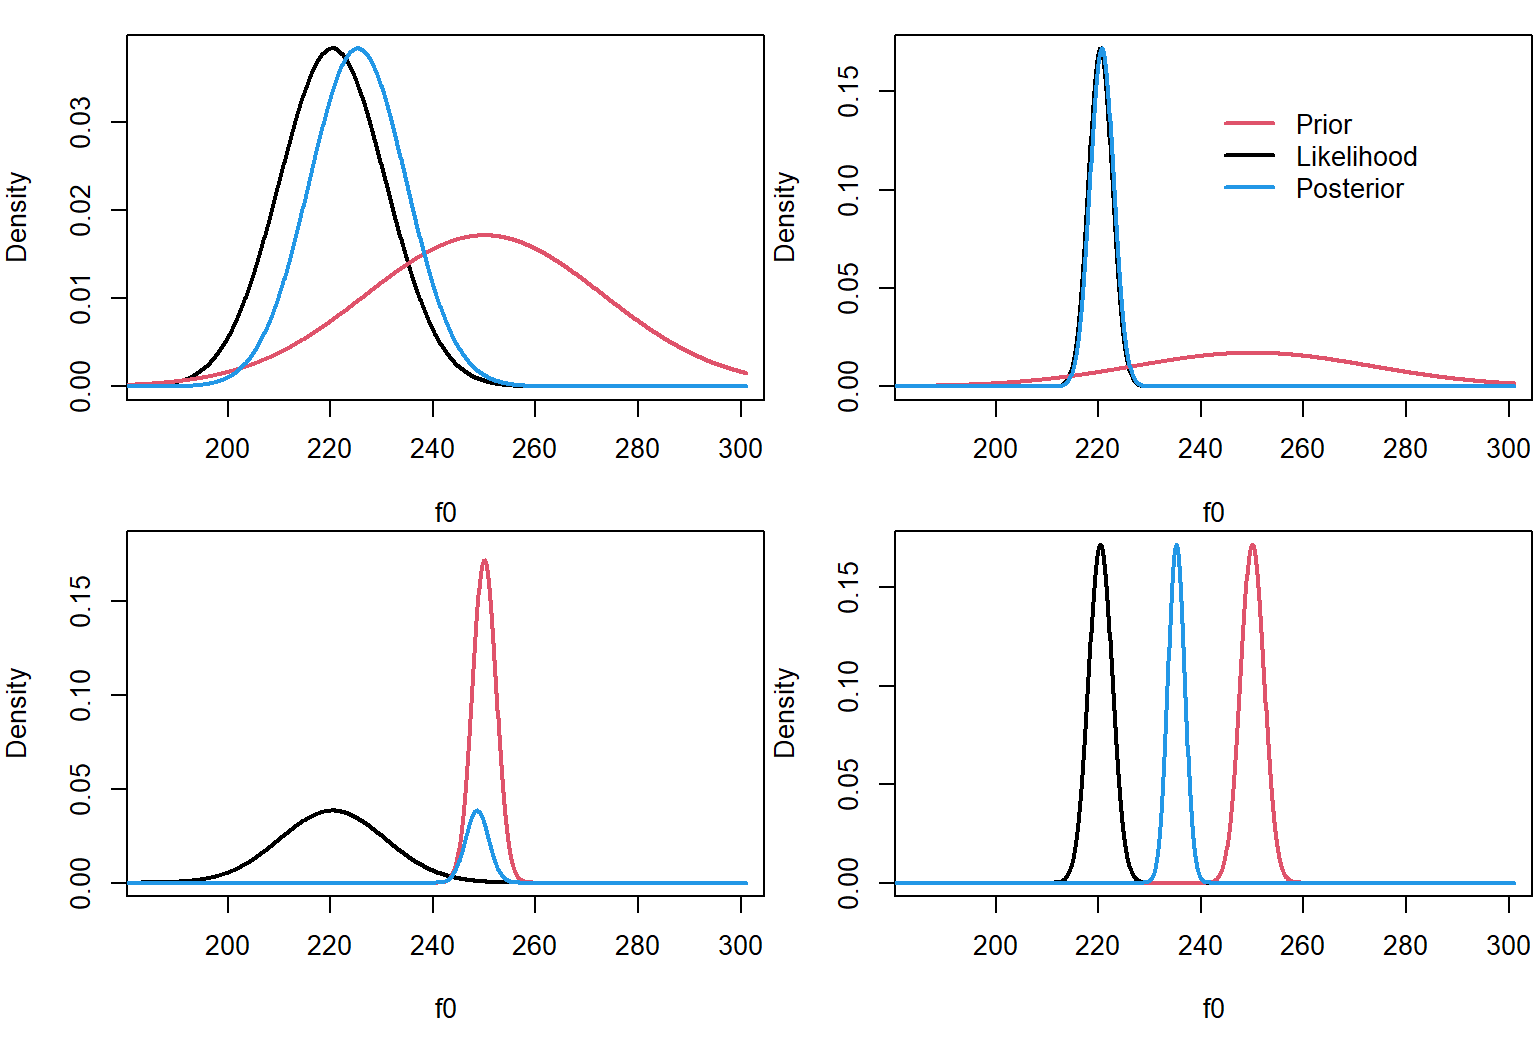
\includegraphics{01_files/figure-latex/F1-posterior-1.pdf}
\caption{\label{fig:F1-posterior}Demonstration of the effect of different types of priors and likelihoods on posterior distributions.}
\end{figure}

\hypertarget{sampling-from-the-posterior}{%
\subsection{Sampling from the posterior}\label{sampling-from-the-posterior}}

We want to understand the posterior distribution of parameters. How do we get this information? It is difficult to get this \emph{analytically}, that is, using exact methods and solving a bunch of equations. Many traditional methods can actually be solved in this way, and that is a big part of their popularity.

Understanding the characteristics of posterior probabilities is not possible analytically for many Bayesian models. As a result, these questions are answered `numerically', basically by using a bunch of `guesses'. To understand the properties of posterior distributions, we use `sampling' software that knows how to investigate these distributions.

You do not need to understand any of this section to use and understand Bayesian multilevel models, the software we will be using will do all of this for us. I am only presenting this to demystify them a little.

The way these samplers work is you specify a set of data and some relationships you think are represented in your data (i.e., a model). The sampler then `walks around' the parameter space, which is the range of possible values a parameter (or set of parameters) can take. For example, for a single parameter the parameter space is a line (like the x axis in the plots above) along which the parameter varies.

The sampler then does some variant of the following algorithm:

\begin{enumerate}
\def\labelenumi{\arabic{enumi})}
\item
  Pick a random value for the parameter (i.e., \(\mu_{tmp}\) = 221 Hz).
\item
  Calculate the posterior probability for the current estimate of \(\mu_{tmp}\).
\item
  If the posterior estimate meets some criteria (e.g., it is better than the last one, it is not too low, etc.), then the value of \(\mu_{tmp}\) is recorded, and becomes \(\mu_{estimate}\). If not it is just discarded.
\item
  Go back to step 1.
\end{enumerate}

As incredible, and magical, as it may seem, under a very reasonable set of conditions if you do the above enough times, the distribution of \(\mu_{estimate}\) that results from the above process will converge on the posterior distribution of \(\mu\) given your data and model structure (including prior probabilities).

Below I have made a small example of this process. I use the Metropolis-Hastings algorithm, which is an algorithm to sample from probability distributions. The small example below assumes the standard deviation of the population is known, and just tries to investigate the posterior distribution of \(\mu\). It uses a very broad prior distribution (\(\mu = 0\), \(\sigma = 5000\)) so that it will have a very weak effect on the outcomes.

\begin{Shaded}
\begin{Highlighting}[]
\CommentTok{\# the function below takes a random sample, an initial mean estimate and a fixed}
\CommentTok{\# standard deviation. It then takes a certain amount of samples from the }
\CommentTok{\# posterior distribution of the parameter, assuming a broad prior centered at 0}
\NormalTok{sampler\_example }\OtherTok{=} \ControlFlowTok{function}\NormalTok{ (sample, }\AttributeTok{mu\_estimate =} \DecValTok{0}\NormalTok{, }\AttributeTok{stdev =} \DecValTok{1}\NormalTok{, }\AttributeTok{nsamples =} \DecValTok{1000}\NormalTok{)\{}
  \CommentTok{\# initial posterior calculation. This is the sum of the log likelihood and}
  \CommentTok{\# the logarithm of the prior probability.}
\NormalTok{  prior }\OtherTok{=} \FunctionTok{log}\NormalTok{ (}\FunctionTok{dnorm}\NormalTok{ (mu\_estimate[}\DecValTok{1}\NormalTok{],}\DecValTok{0}\NormalTok{, }\DecValTok{500}\NormalTok{))}
\NormalTok{  loglik }\OtherTok{=} \FunctionTok{sum}\NormalTok{ (}\FunctionTok{dnorm}\NormalTok{ (sample, mu\_estimate[}\DecValTok{1}\NormalTok{],stdev,}\AttributeTok{log=}\ConstantTok{TRUE}\NormalTok{))}
\NormalTok{  old\_posterior }\OtherTok{=}\NormalTok{ loglik }\SpecialCharTok{+}\NormalTok{ prior}
  
  \ControlFlowTok{for}\NormalTok{ (i }\ControlFlowTok{in} \DecValTok{2}\SpecialCharTok{:}\NormalTok{nsamples)\{}
\NormalTok{    accept }\OtherTok{=} \ConstantTok{FALSE}
    \CommentTok{\# this loop will keep proposing new steps until one gets accepted. }
    \ControlFlowTok{while}\NormalTok{ (}\SpecialCharTok{!}\NormalTok{accept)\{}
      \CommentTok{\# (step 1 above)}
      \CommentTok{\# draw new proposal by randomly changing the previous mu\_estimate}
\NormalTok{      mu\_tmp }\OtherTok{=}\NormalTok{ mu\_estimate[i}\DecValTok{{-}1}\NormalTok{] }\SpecialCharTok{+} \FunctionTok{rnorm}\NormalTok{ (}\DecValTok{1}\NormalTok{, }\DecValTok{0}\NormalTok{, .}\DecValTok{3}\NormalTok{)}
      \CommentTok{\# (step 2 above)}
      \CommentTok{\# find prior probability for new mu\_tmp proposal}
\NormalTok{      prior }\OtherTok{=} \FunctionTok{log}\NormalTok{ (}\FunctionTok{dnorm}\NormalTok{ (mu\_tmp,}\DecValTok{0}\NormalTok{, }\DecValTok{500}\NormalTok{))}
      \CommentTok{\# find log likelihood for new mu\_tmp proposal}
\NormalTok{      loglik }\OtherTok{=} \FunctionTok{sum}\NormalTok{ (}\FunctionTok{dnorm}\NormalTok{ (sample, mu\_tmp,stdev,}\AttributeTok{log=}\ConstantTok{TRUE}\NormalTok{))}
      \CommentTok{\# calculate the new posterior probability}
\NormalTok{      new\_posterior }\OtherTok{=}\NormalTok{ prior }\SpecialCharTok{+}\NormalTok{ loglik}
      \CommentTok{\# (step 3 above)}
      \CommentTok{\# if better accept always. If worse, accept sometimes}
      \ControlFlowTok{if}\NormalTok{ ( ( new\_posterior }\SpecialCharTok{{-}}\NormalTok{ old\_posterior ) }\SpecialCharTok{\textgreater{}=} \FunctionTok{log}\NormalTok{ ( }\FunctionTok{runif}\NormalTok{ (}\DecValTok{1}\NormalTok{,}\DecValTok{0}\NormalTok{,}\DecValTok{1}\NormalTok{) ) )\{}
\NormalTok{        mu\_estimate[i] }\OtherTok{=}\NormalTok{ mu\_tmp}
        \CommentTok{\# if you accept, the new estimate becomes the current estimate}
\NormalTok{        old\_posterior }\OtherTok{=}\NormalTok{ new\_posterior}
\NormalTok{        accept }\OtherTok{=} \ConstantTok{TRUE}
\NormalTok{      \}}
\NormalTok{    \}}
\NormalTok{  \} }
  \FunctionTok{return}\NormalTok{ (mu\_estimate)}
\NormalTok{\}}
\end{Highlighting}
\end{Shaded}

In the plots below, I show this algorithm at work. In the top row, a random sample with a mean of -50 is used. You can see that the sampler starts at 0 but quickly finds the sample mean (left column). In the middle, I show the distribution of the samples on the left, minus the section it uses to `find' the parameter value (called the `burn-in phase'). On the right, I compare our samples (blue) to the theoretical posterior distribution for the mean given the data and prior (red). I toss out the samples during the `burn in' phase, as there are used up in trying to `find' the correct location in the parameter space.

In the bottom row, I use this algorithm on our f0 data! This is a `Bayesian' analysis since it combines information about parameter likelihood and prior probabilities. We can also see that even this simple approach yields a good correspondence to the theoretical posterior distribution of the parameter, and results in broadly the same conclusions we have arrived at by other means.

\begin{figure}
\centering
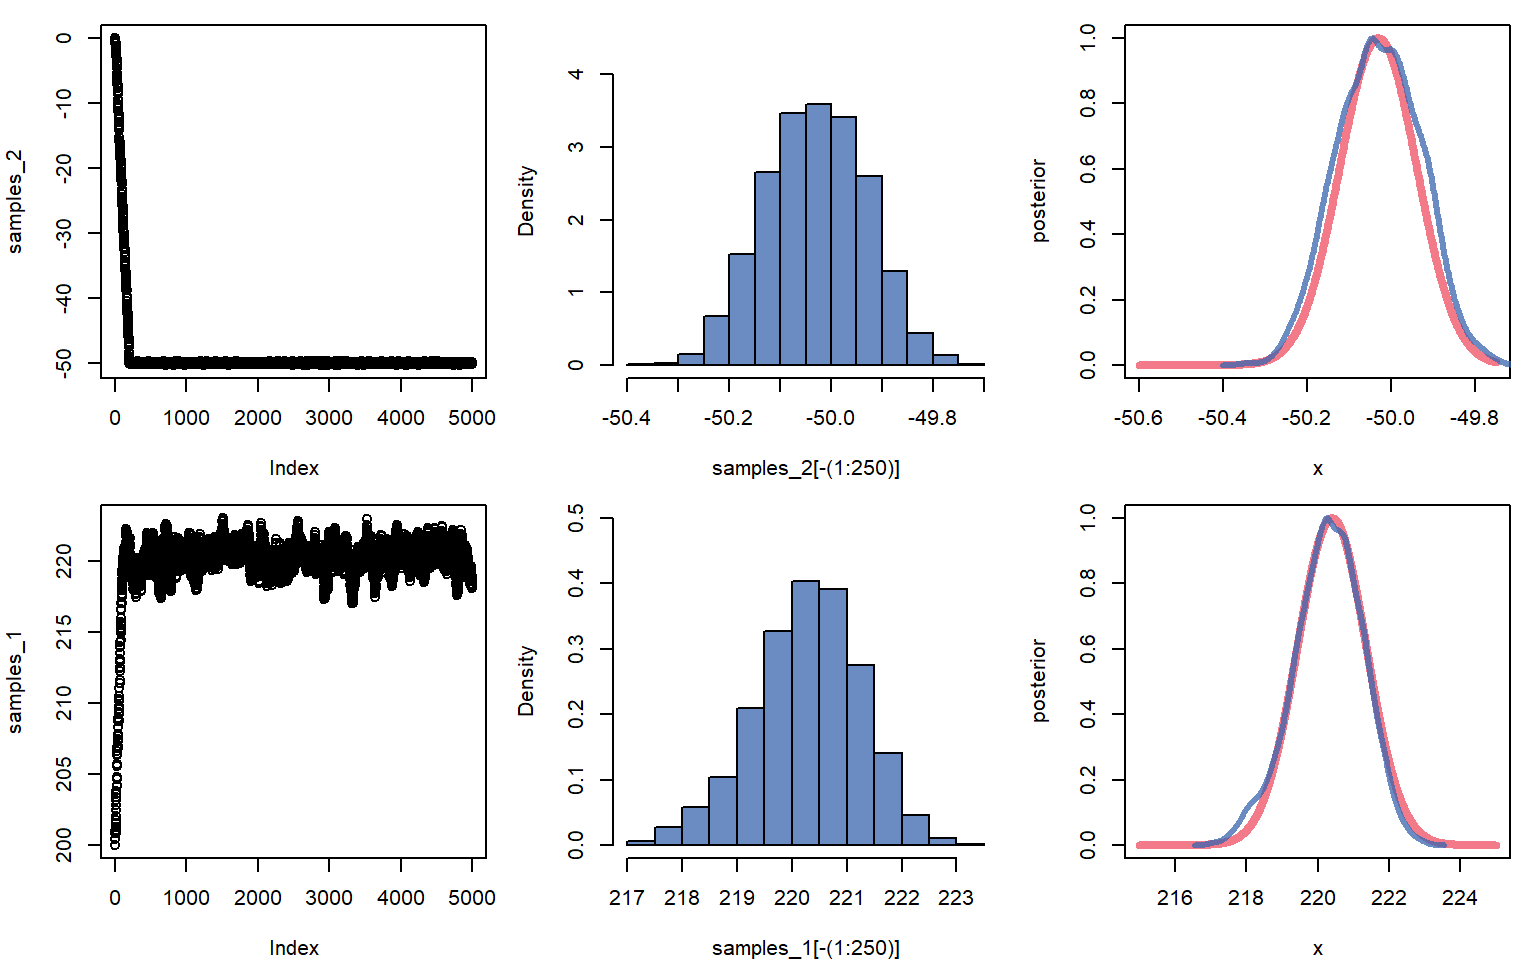
\includegraphics{01_files/figure-latex/F1-mcmc-1.pdf}
\caption{\label{fig:F1-mcmc}Demonstration of parameter estimation using a random walk, yielding a good approximation of analytically-derived values.}
\end{figure}

The results clearly coincide, but aren't perfect. But this sampler isn't very sophisticated! The samplers we will be using in this class \emph{do} provide an excellent match to the posterior distribution. As a result, we can inspect the distribution of collected \(\mu_{estimate}\) to understand the posterior of our parameter. We can use these distributions in the same way that we used the theoretical likelihood functions above, by using them to make statements about likely parameter values and ranges of values.

\hypertarget{exercises}{%
\section{Exercises}\label{exercises}}

There is no modeling in this chapter, and the focus is on presenting some fundamental concepts. In Chapter 2 we will begin fitting Bayesian multilevel models to data. This book does not really go into very much detail about the usage of R, and it instead assumes a basic familiarity with the software.

In place of statistical exercises, the time devoted to this chapter can be used to make sure that the reader (or student or class) has a reasonable understanding of R and a basic familiarity with the important data structures in R (e.g., vectors, dataframes), and some of the more basic functionalities of the software.

\hypertarget{inspecting-a-single-group-of-observations-using-a-bayesian-multilevel-model}{%
\chapter{Inspecting a `single group' of observations using a Bayesian multilevel model}\label{inspecting-a-single-group-of-observations-using-a-bayesian-multilevel-model}}

The previous chapter was mostly introductory, it introduced some basic terminology and concepts that are required to begin talking about models. In this chapter we are going to return to questions like 'what is the average value of \(x\), however, in this chapter we are going to learn to answer these questions using Bayesian multilevel regression models in R using the \texttt{brms} package.

The models discussed in this chapter can be used for data that comes from a single group of subjects. By a `single' group I just mean that you are not trying to compare things here, you are just trying to understand the average values of some variable for a single group of observations. The data:

\begin{itemize}
\tightlist
\item
  comes from from one speaker/subject or many speakers/subjects.
\item
  each speaker/subject can contribute multiple data points, and the number does not need to be balanced across subjects.
\end{itemize}

The `traditional' design equivalent to these models is a one-sample t-test, although the Bayesian approach has many advantages (as discussed at the end of the chapter).

\hypertarget{data-and-research-questions-1}{%
\section{Data and research questions}\label{data-and-research-questions-1}}

We're going to keep analyzing the female f0 data from the Hillenbrand et al.~(1995) dataset, discussed in chapter 1. These are 576 observations, 12 production collected from each of 48 women in the sample. So, our data comes from multiple speakers and we has multiple observations from each speaker, and the women are in the single group ``adult women form Michigan''. Of course, we could divide these women into any number of smaller groups based on hair color, handedness, and so on. These women are considered to be in a single group because our model, our \emph{conceptualization} of these speakers, places them in a single group.

We're going to try to address the same questions we talked about last week:

\begin{enumerate}
\def\labelenumi{\arabic{enumi})}
\item
  What is the average f0 of the whole \emph{population} likely to be?
\item
  Can we set bounds on likely mean f0 values based on the data we collected?
\end{enumerate}

However, this time we are going to do this with a Bayesian multilevel model. We're going to see how the model provides us with the same information we got in the last chapter, in addition to providing us with additional useful information.

\hypertarget{estimating-a-single-mean-with-the-brms-package}{%
\section{\texorpdfstring{Estimating a single mean with the \texttt{brms} package}{Estimating a single mean with the brms package}}\label{estimating-a-single-mean-with-the-brms-package}}

The \texttt{brms} \href{https://github.com/paul-buerkner/brms}{(`Bayesian regression models')} package in R lets you fit Bayesian models using the STAN probabilistic programming language using R. The package is really amazing and makes Bayesian multilevel modeling easy and accessible for anyone. It also includes a lot of helper functions that make working with these models very convenient.

\texttt{brms} should be installed in R so that the models described below will work. Make sure you have the latest version of R (and Rstudio) and the latest version of the \texttt{brms} package installed. Sometimes using older versions can cause R to crash when fitting models. Anecdotal experience suggests that if all of the sudden trying to fit these models causes crashes or mysterious errors, its time to update one or more of R, Rstudio, or \texttt{brms}.

\hypertarget{description-of-the-model}{%
\subsection{Description of the model}\label{description-of-the-model}}

We're going to learn to read and write formal descriptions of our models. The notation we will learn will help us describe our models efficiently, and it will help us understand the models used by other people.

The relationship between statistical concepts and the formal notation used to represent them is very similar to musical notation and the ability to play music. Someone who can play a song undoubtedly \emph{knows} that song. However, in the absence of formal musical training that same person might not recognize sheet music recognizing the song. The person would also lack the vocabulary to discuss components of the song, and may find it difficult to learn to play new pieces. In the same way, most people have excellent intuitive understanding of many statistical concepts such as slopes, interactions, error, and so on. However, they lack the notational knowledge to understand these relations when expressed in the formal notation often used to express these ideas.

Recall from Chapter 1 that our `model' for a single group of normally distributed values can be thought of in one of two two ways:

\begin{equation}
\begin{split}
\\
y_{[i]} = \mu_{[i]} + \varepsilon_{[i]} \\ \\
y_{[i]} \sim \mathcal{N}(\mu_{[i]},\sigma) \\ \\
\end{split}
\label{eq:21}
\end{equation}

The top line says that your observed variable for any given trial \(y_{[i]}\) is the sum of some of some average expected value for that trial, (\(\mu_{[i]}\)) and some specific random error for that trial (\(\varepsilon_{[i]}\)). The random error is expected to be normally distributed with a mean of 0 and some unknown standard deviation (as in: \(\varepsilon_{[i]} \sim \mathcal{N}(0,\sigma)\)). The second line presents the \(y\) variable as being a normally-distributed variable with a trial-specific mean of \(\mu_i\), and a fixed standard deviation \(\sigma_{error}\)

In general, we use regression models to understand orderly variation in \(\mu_{[i]}\) from trial to trial by breaking it up into predictors (\(\mathrm{x}_{1}, \mathrm{x}_{2},...\)) that are combined using some weights (\(\alpha_1, \alpha_2,...\)). If this statement makes no sense please see Chapter 1!.

\[
\mu_{[i]} = \alpha_1*\mathrm{x}_{1{[i]}} + \alpha_2*\mathrm{x}_{2i}+...+\alpha_j*\mathrm{x}_{j{[i]}}
\label{eq:22}
\]

`Fitting' a regression model consists of trying to `guess' the values of the weighing factors (\(\alpha\)), called the \emph{model coefficients}. When we are only trying to estimate a single average, we don't have any predictors to explain variation in \(\mu_{[i]}\). In fact, our model structure suggests we expect no variation in \(\mu_{[i]}\) from trial to trial!.

Mathematically, we can't just say `we have no predictor' since everything needs to be represented by a number. As a result, we use a single `predictor' \(\mathrm{x}\) with a value of 1 so that our regression equation is:

\[
\mu_{[i]} = \alpha_1*1
\label{eq:23}
\]

Now our model is trying to guess the value of a single coefficient (\(\alpha_1\)), and we expect this coefficient to be equal to \(\mu_{[i]}\) since it is being multiplied by a `predictor' with a constant value of 1.

This kind of model is called an `Intercept only' model. Regression models are really about representing \emph{differences}, differences between groups and across conditions. When you are encoding differences, you need an overall reference point. For example, saying that something is 5 miles north is only interpretable given some reference point. The `reference point' used by your model is called your `Intercept', it is the center of your model's universe.

Basically, our model consists \emph{only} of a single reference point, and the \(\alpha_1\) parameter reflects its value (as shown in Equation \eqref{eq:23}). As a result, the \(\alpha_1\) coefficient is called the `intercept' in our model. When a coefficient is just being multiplied by a `fake' predictor that just equals 1, we can omit it from the regression model (but its still secretly there).

Based on the above, our model investigating the f0 produced by adult women from Michigan can be thought of like this:

\begin{equation}
\begin{split}
\\
f0_{[i]} \sim \mathcal{N}(\mu_{[i]},\sigma) \\ \\ 
\mu_{[i]} = Intercept \\ \\
\end{split}
\label{eq:24}
\end{equation}

Put in plain English, each line in the model says the following:

\begin{itemize}
\item
  We expect that f0 for a given observation \(i\) is normally distributed according to some trial-specific expected value and some unknown (but fixed) standard deviation.
\item
  The expected value for any given trial (\(\mu_{[i]}\)) is equal to the intercept of the model for all trials. This means its fixed and we have the same expected value for all tokens!
\end{itemize}

What the model also implicitly says that the error is drawn from a normal distribution with a mean of 0 and a standard deviation of \(\sigma\). This distribution represents all deviations in f0 around the mean f0 for the sample (\(\mu_{[i]}\)). In other words, the error for this model is expected to look like:

\[
\varepsilon_{[i]} \sim \mathcal{N}(0,\sigma)
\label{eq:25}
\]

\hypertarget{the-model-formula}{%
\subsection{The model formula}\label{the-model-formula}}

Model structures are expressed in R using a very specific syntax. Think of writing a model formula as writing a language within R. Generally, model formulas in R have the form:

\texttt{y\ \textasciitilde{}\ predictors}

The variable we are interested in understanding (\(y\)) goes on the left hand side of the \(\sim\), and on our predictors go on the right hand side. Notice that the random term (\(\varepsilon\)) is not included in the model formula.

The formula above can be read as `y is distributed according to some predictor', which really means ``we think there is systematic variation in our y variable that can be understood by considering its joint variation with our predictor variable(s).''

For intercept only models, the number \texttt{1} is included in the model formula to indicate that a single constant value is being estimated (as in \eqref{eq:23}). As a result, our model formula will have the form:

\texttt{f0\ \textasciitilde{}\ 1}

This model could be said out loud like ``we are trying to estimate the mean of f0'' or ``we are predicting mean f0 given only an intercept''.

\hypertarget{fitting-the-model-calling-the-brm-function}{%
\subsection{\texorpdfstring{Fitting the model: Calling the \texttt{brm} function}{Fitting the model: Calling the brm function}}\label{fitting-the-model-calling-the-brm-function}}

Below, I load the \texttt{brms} package, which contains the \texttt{brm} function. The \texttt{brm} function takes a model specification, data and some other information, and fits a model that estimates all the model parameters. Unless otherwise specified, \texttt{brm} assumes that the error component (\(\varepsilon\)) of your model is normally distributed. The first argument in the function call is the model formula, and the second argument tells the function where to find the data (a dataframe called \texttt{w}). The other arguments tell the function to estimates a single set of samples (chains = 1) using a single processor on your CPU (cores = 1). These arguments will be discussed more later.

\begin{Shaded}
\begin{Highlighting}[]
\CommentTok{\# Get data from course website}
\NormalTok{url1 }\OtherTok{=} \StringTok{"https://raw.githubusercontent.com/santiagobarreda"}
\NormalTok{url2 }\OtherTok{=} \StringTok{"/stats{-}class/master/data/h95\_vowel\_data.csv"}
\NormalTok{h95 }\OtherTok{=} \FunctionTok{read.csv}\NormalTok{ (}\FunctionTok{url}\NormalTok{(}\FunctionTok{paste0}\NormalTok{ (url1, url2)))}
\CommentTok{\# select women only}
\NormalTok{w }\OtherTok{=}\NormalTok{ h95[h95}\SpecialCharTok{$}\NormalTok{group }\SpecialCharTok{==} \StringTok{\textquotesingle{}w\textquotesingle{}}\NormalTok{,]}

\CommentTok{\# To ensure predictable results in examples, I will be using the same random  }
\CommentTok{\# seed throughout, and resetting it before running any \textquotesingle{}random\textquotesingle{} process.  }
\FunctionTok{set.seed}\NormalTok{ (}\DecValTok{1}\NormalTok{)}
\NormalTok{model }\OtherTok{=}\NormalTok{ brms}\SpecialCharTok{::}\FunctionTok{brm}\NormalTok{ (f0 }\SpecialCharTok{\textasciitilde{}} \DecValTok{1}\NormalTok{, }\AttributeTok{data =}\NormalTok{ w, }\AttributeTok{chains =} \DecValTok{1}\NormalTok{, }\AttributeTok{cores =} \DecValTok{1}\NormalTok{)}

\DocumentationTok{\#\# SAMPLING FOR MODEL \textquotesingle{}77bdac4488ef47de193e19dae81fc150\textquotesingle{} NOW (CHAIN 1).}
\DocumentationTok{\#\# Chain 1: }
\DocumentationTok{\#\# Chain 1: Gradient evaluation took 0 seconds}
\DocumentationTok{\#\# Chain 1: 1000 transitions using 10 leapfrog steps per transition would take 0 seconds.}
\DocumentationTok{\#\# Chain 1: Adjust your expectations accordingly!}
\DocumentationTok{\#\# Chain 1: }
\DocumentationTok{\#\# Chain 1: }
\DocumentationTok{\#\# Chain 1: Iteration:    1 / 2000 [  0\%]  (Warmup)}
\DocumentationTok{\#\# Chain 1: Iteration:  200 / 2000 [ 10\%]  (Warmup)}
\DocumentationTok{\#\# Chain 1: Iteration:  400 / 2000 [ 20\%]  (Warmup)}
\DocumentationTok{\#\# Chain 1: Iteration:  600 / 2000 [ 30\%]  (Warmup)}
\DocumentationTok{\#\# Chain 1: Iteration:  800 / 2000 [ 40\%]  (Warmup)}
\DocumentationTok{\#\# Chain 1: Iteration: 1000 / 2000 [ 50\%]  (Warmup)}
\DocumentationTok{\#\# Chain 1: Iteration: 1001 / 2000 [ 50\%]  (Sampling)}
\DocumentationTok{\#\# Chain 1: Iteration: 1200 / 2000 [ 60\%]  (Sampling)}
\DocumentationTok{\#\# Chain 1: Iteration: 1400 / 2000 [ 70\%]  (Sampling)}
\DocumentationTok{\#\# Chain 1: Iteration: 1600 / 2000 [ 80\%]  (Sampling)}
\DocumentationTok{\#\# Chain 1: Iteration: 1800 / 2000 [ 90\%]  (Sampling)}
\DocumentationTok{\#\# Chain 1: Iteration: 2000 / 2000 [100\%]  (Sampling)}
\DocumentationTok{\#\# Chain 1: }
\DocumentationTok{\#\# Chain 1:  Elapsed Time: 0.08 seconds (Warm{-}up)}
\DocumentationTok{\#\# Chain 1:                0.058 seconds (Sampling)}
\DocumentationTok{\#\# Chain 1:                0.138 seconds (Total)}
\DocumentationTok{\#\# Chain 1: }
\end{Highlighting}
\end{Shaded}

By default, \texttt{brms} takes 2000 samples, throwing out the first 1000 and returning the last 1000. The output above shows you that the sampler is working, and tells you about the progress as it works. This is a small amount of data so it should be pretty fast.

This is the last time I will be actually fitting a model in the code chunks. I am going to be relying on pre-fit models that you can load after downloading from the course GitHub. Models can be found in the folder corresponding to each chapter.

\begin{Shaded}
\begin{Highlighting}[]
\CommentTok{\# download pre{-}fit model from: }
\CommentTok{\# github.com/santiagobarreda/stats{-}class/tree/master/models}
\CommentTok{\# and load after placing in working directory}
\NormalTok{model }\OtherTok{=} \FunctionTok{readRDS}\NormalTok{ (}\StringTok{\textquotesingle{}2\_model.RDS\textquotesingle{}}\NormalTok{)}
\end{Highlighting}
\end{Shaded}

\hypertarget{interpreting-the-model-the-print-statement}{%
\subsection{Interpreting the model: the print statement}\label{interpreting-the-model-the-print-statement}}

Typing the model name into the console and hitting enter prints the default \texttt{brms} model print statement:

\begin{Shaded}
\begin{Highlighting}[]
\CommentTok{\# inspect model}
\NormalTok{model}
\DocumentationTok{\#\#  Family: gaussian }
\DocumentationTok{\#\#   Links: mu = identity; sigma = identity }
\DocumentationTok{\#\# Formula: f0 \textasciitilde{} 1 }
\DocumentationTok{\#\#    Data: w (Number of observations: 576) }
\DocumentationTok{\#\# Samples: 1 chains, each with iter = 2000; warmup = 1000; thin = 1;}
\DocumentationTok{\#\#          total post{-}warmup samples = 1000}
\DocumentationTok{\#\# }
\DocumentationTok{\#\# Population{-}Level Effects: }
\DocumentationTok{\#\#           Estimate Est.Error l{-}95\% CI u{-}95\% CI Rhat Bulk\_ESS Tail\_ESS}
\DocumentationTok{\#\# Intercept   220.40      0.97   218.33   222.30 1.00      851      557}
\DocumentationTok{\#\# }
\DocumentationTok{\#\# Family Specific Parameters: }
\DocumentationTok{\#\#       Estimate Est.Error l{-}95\% CI u{-}95\% CI Rhat Bulk\_ESS Tail\_ESS}
\DocumentationTok{\#\# sigma    23.24      0.69    21.99    24.61 1.00      653      550}
\DocumentationTok{\#\# }
\DocumentationTok{\#\# Samples were drawn using sampling(NUTS). For each parameter, Bulk\_ESS}
\DocumentationTok{\#\# and Tail\_ESS are effective sample size measures, and Rhat is the potential}
\DocumentationTok{\#\# scale reduction factor on split chains (at convergence, Rhat = 1).}
\end{Highlighting}
\end{Shaded}

The first part just tells you some technical details that we don't have to worry about for now (though some are obvious).

\begin{Shaded}
\begin{Highlighting}[]
\DocumentationTok{\#\#  Family: gaussian }
\DocumentationTok{\#\#   Links: mu = identity; sigma = identity }
\DocumentationTok{\#\# Formula: f0 \textasciitilde{} 1 }
\DocumentationTok{\#\#    Data: w (Number of observations: 576) }
\DocumentationTok{\#\# Samples: 1 chains, each with iter = 2000; warmup = 1000; thin = 1;}
\DocumentationTok{\#\#          total post{-}warmup samples = 1000}
\end{Highlighting}
\end{Shaded}

Next we see estimated effects for out predictors, in this case only an intercept. This is a `population' level effect because is is shared by all observations in our sample, and not specific to any one observation.

\begin{Shaded}
\begin{Highlighting}[]
\DocumentationTok{\#\# Population{-}Level Effects: }
\DocumentationTok{\#\#           Estimate Est.Error l{-}95\% CI u{-}95\% CI Rhat Bulk\_ESS Tail\_ESS}
\DocumentationTok{\#\# Intercept   220.40      0.97   218.33   222.30 1.00      851      557}
\end{Highlighting}
\end{Shaded}

The information above provides the mean (Estimate) and standard deviation (Est. Error) of the posterior distribution of \(\mu\) (\texttt{Intercept}). The values of \texttt{l-95\%\ CI} and \texttt{u-95\%\ CI} represent the upper and lower `95\% credible intervals' for the posterior distribution of this parameter.

The \emph{X\% credible interval} for a parameter is the smallest interval that encloses X\% of the distribution. This parameter has an X\% chance (0.X probability) of falling inside the X\% credible interval. So, this means that there is a 95\% probability that \(\mu\) is between 218 and 222 Hz given our data and model structure.

Notice that the parameter estimate and intervals almost exactly match the estimate and intervals we obtain by referencing the theoretical likelihood function (discussed in Chapter 1):

\begin{Shaded}
\begin{Highlighting}[]
\CommentTok{\# sample mean}
\FunctionTok{mean}\NormalTok{ (f0)}
\DocumentationTok{\#\# [1] 220.401}

\CommentTok{\# theoretical quantiles for likelihood of mean}
\FunctionTok{qnorm}\NormalTok{ (}\FunctionTok{c}\NormalTok{(}\FloatTok{0.025}\NormalTok{, }\FloatTok{0.975}\NormalTok{), }\FunctionTok{mean}\NormalTok{ (f0), }\FunctionTok{sd}\NormalTok{ (f0) }\SpecialCharTok{/} \FunctionTok{sqrt}\NormalTok{ (}\FunctionTok{length}\NormalTok{ (f0) ) )}
\DocumentationTok{\#\# [1] 218.5047 222.2974}
\end{Highlighting}
\end{Shaded}

As noted in Chapter 1, `frequentist' and `Bayesian' estimation differ in terms of whether they rely on the posterior or likelihoods to make inferences. However, for most real cases we expect the posterior to be dominated by the likelihood (see \ref{fig:F1-posterior}, and as a result we expect Bayesian and frequentist estimation to provide roughly equivalent answers given equivalent model structures.

Our model also provides us an estimate of the error standard deviation(\(\sigma\)), under `Family Specific Parameters: sigma'. This estimate closely matches our sample standard deviation estimate (\texttt{sd(f0)}) of 23.2 Hz. In addition, we also get a 95\% credible interval for this parameter (2.5\% = 21.99, 97.5\% = 24.61).

\begin{Shaded}
\begin{Highlighting}[]
\DocumentationTok{\#\# Family Specific Parameters: }
\DocumentationTok{\#\#       Estimate Est.Error l{-}95\% CI u{-}95\% CI Rhat Bulk\_ESS Tail\_ESS}
\DocumentationTok{\#\# sigma    23.24      0.69    21.99    24.61 1.00      653      550}
\end{Highlighting}
\end{Shaded}

This last section is just boilerplate and contains some basic reminders. This text will look the same after all models.

\begin{Shaded}
\begin{Highlighting}[]
\DocumentationTok{\#\# Samples were drawn using sampling(NUTS). For each parameter, Bulk\_ESS}
\DocumentationTok{\#\# and Tail\_ESS are effective sample size measures, and Rhat is the potential}
\DocumentationTok{\#\# scale reduction factor on split chains (at convergence, Rhat = 1).}
\end{Highlighting}
\end{Shaded}

\hypertarget{seeing-the-samples}{%
\subsection{Seeing the samples}\label{seeing-the-samples}}

In Chapter 1 I discussed that samplers (like \texttt{brm}, or STAN) take samples of the posterior distributions of parameters given the data and model structure. It's helpful to see that this is quite literally what is happening, and that the print statement above just summarizes the information contained in the posterior samples. Actually, one of the great things about Bayesian models is that you can make your own summaries of the posterior samples, and summarize them in several ways as required.

Below I get the posterior samples from the model. We have 1000 samples, as indicated in the model output above. The first column represents the model intercept (\texttt{b\_Intercept}), the middle column is the error (\texttt{sigma}), and the third column is a statistic related to model fit (\texttt{lp\_\_}).

\begin{Shaded}
\begin{Highlighting}[]
\CommentTok{\# get posterior samples from model}
\NormalTok{samples }\OtherTok{=}\NormalTok{ brms}\SpecialCharTok{::}\FunctionTok{posterior\_samples}\NormalTok{ (model)}
\FunctionTok{str}\NormalTok{ (samples)}
\DocumentationTok{\#\# \textquotesingle{}data.frame\textquotesingle{}:    1000 obs. of  3 variables:}
\DocumentationTok{\#\#  $ b\_Intercept: num  221 221 220 222 220 ...}
\DocumentationTok{\#\#  $ sigma      : num  22.1 21.9 23.2 21.9 22.9 ...}
\DocumentationTok{\#\#  $ lp\_\_       : num  {-}2635 {-}2635 {-}2634 {-}2637 {-}2634 ...}
\end{Highlighting}
\end{Shaded}

We can plot the individual samples for the mean parameter on the left below. On the right I plot a histogram of the same samples, superimposed with the theoretical distribution of the likelihood we calculated in Chapter 1.

\begin{figure}
\centering
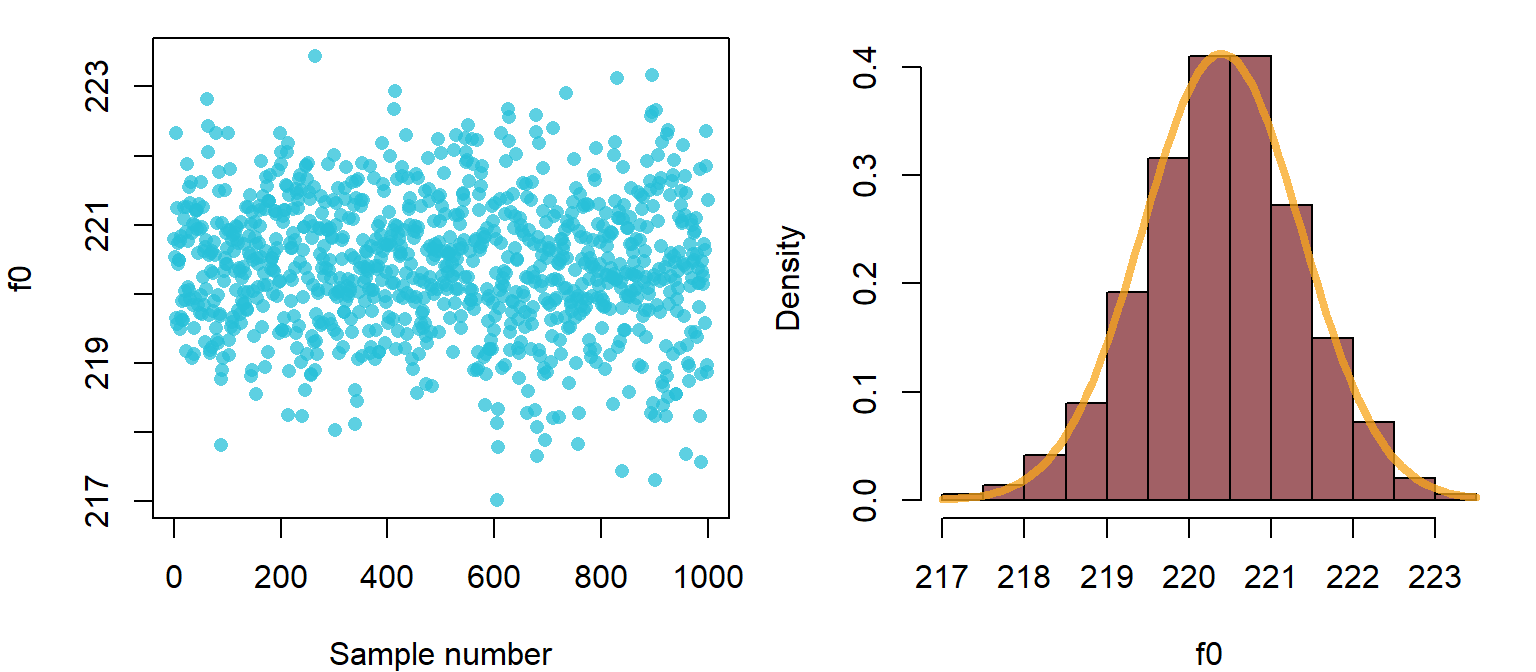
\includegraphics{02_files/figure-latex/F2-1-1.pdf}
\caption{\label{fig:F2-1}(left) Individual samples from posterior of mean f0 parameter. (right) a histogram of the same samples.}
\end{figure}

Recall that our model output provides information about expected values for the mean parameter:

\begin{Shaded}
\begin{Highlighting}[]
\DocumentationTok{\#\# Population{-}Level Effects: }
\DocumentationTok{\#\#           Estimate Est.Error l{-}95\% CI u{-}95\% CI Rhat Bulk\_ESS Tail\_ESS}
\DocumentationTok{\#\# Intercept   220.40      0.97   218.33   222.30 1.00      851      557}
\end{Highlighting}
\end{Shaded}

These simply correspond to the quantiles of the posterior samples! We can confirm this by checking the quantiles on the vector containing the posterior samples for the mean parameter as below:

\begin{Shaded}
\begin{Highlighting}[]
\FunctionTok{quantile}\NormalTok{ (samples[,}\StringTok{"b\_Intercept"}\NormalTok{], }\FunctionTok{c}\NormalTok{(.}\DecValTok{025}\NormalTok{, .}\DecValTok{5}\NormalTok{, .}\DecValTok{975}\NormalTok{))}
\DocumentationTok{\#\#     2.5\%      50\%    97.5\% }
\DocumentationTok{\#\# 218.3288 220.3997 222.3001}
\end{Highlighting}
\end{Shaded}

And we can see that these exactly correspond to the values of \texttt{Estimate}, \texttt{l-95\%\ CI}, and \texttt{u-95\%\ CI} in the model print statement above. There is no special status for these quantiles. We can check the values of other ones:

\begin{Shaded}
\begin{Highlighting}[]
\FunctionTok{quantile}\NormalTok{ (samples[,}\StringTok{"b\_Intercept"}\NormalTok{], }\FunctionTok{c}\NormalTok{(.}\DecValTok{25}\NormalTok{, .}\DecValTok{75}\NormalTok{))}
\DocumentationTok{\#\#      25\%      75\% }
\DocumentationTok{\#\# 219.8043 221.0296}
\end{Highlighting}
\end{Shaded}

Or even use the posterior distribution to find the probability that the mean parameter is over/under any arbitrary value:

\begin{Shaded}
\begin{Highlighting}[]
\FunctionTok{sum}\NormalTok{ (samples[,}\StringTok{"b\_Intercept"}\NormalTok{] }\SpecialCharTok{\textless{}} \DecValTok{221}\NormalTok{) }\SpecialCharTok{/} \DecValTok{576}
\DocumentationTok{\#\# [1] 1.284722}
\end{Highlighting}
\end{Shaded}

Let's take a second to think about why this works. Recall that the probability is the odds that something will occur out of all the possible outcomes. Our vector \texttt{samples{[},"b\_Intercept"{]}} represents 1000 observations of a random variable, 1000 possible values of the average f0 produced by adult women from Michigan. If we find the total number of these observations that were below 221 Hz and then divide by the total number of observations (576), we are calculating the probability of observing a mean estimate below 221 Hz. As a result, the calculation above says that there is a 0.74 probability (a 74\% chance) that the mean f0 for female speakers in this population is under 221 Hz, given our data and model structure. We come to this conclusion by finding that 74\% of the posterior samples of the parameter of interest are below 221 Hz.

\hypertarget{repeated-measures-data}{%
\section{Repeated measures data}\label{repeated-measures-data}}

The model we fit above is a reasonable starting point, but it has many weaknesses. Importantly, our data consists of 12 productions from each speaker in our sample, meaning we have `repeated measures' data. However, our model does not contain this information an thinks that the 576 observations in our data are entirely independent. Treating repeated measures data as if it were \emph{not} repeated measures data can cause problems for our inferences. This is because it can give us a warped perspective of how much variability there really is in the sample.

For example, if I told you I had 1,000,000 samples of speech from male speakers from Los Angeles, you may be confident that I can estimate the average f0 male speakers from Los Angeles very accurately. But what if I told you that all these samples were from only three different people? You know instinctively that this makes my data less reliable for making inferences about Los Angeles in general, although it may provide excellent information about these three speakers.

The reason repeated-measures data can cause problems is because the measurements are correlated: multiple measurements from the same person are obviously going to be related to each other. If you measure the height of a tall person today, they will still be tall tomorrow. This can be seen quite clearly below. The top panel shows the distribution of all our f0 measurements. The bottom panel shows speaker boxplots (one for each speaker's data). If we were to `push down' on the bottom panel and collapse all our boxplots into a single distribution, we would end up with the boxplot in the top panel.

These boxplots shows that each speaker has their own average f0, and that their productions tend to vary around their `natural average. As a result, we might have something closer to 48 independent observations (one average value per speaker) than 576. For example, if we look at the top boxplot there appear to be 'outliers' around 150 Hz. In the bottom plot we see that these productions all come from one speaker, and actually reflect her average f0. As a result, it seems that the \emph{speaker} is the outlier, and that the values are actually perfectly average for this speaker.

\begin{figure}
\centering
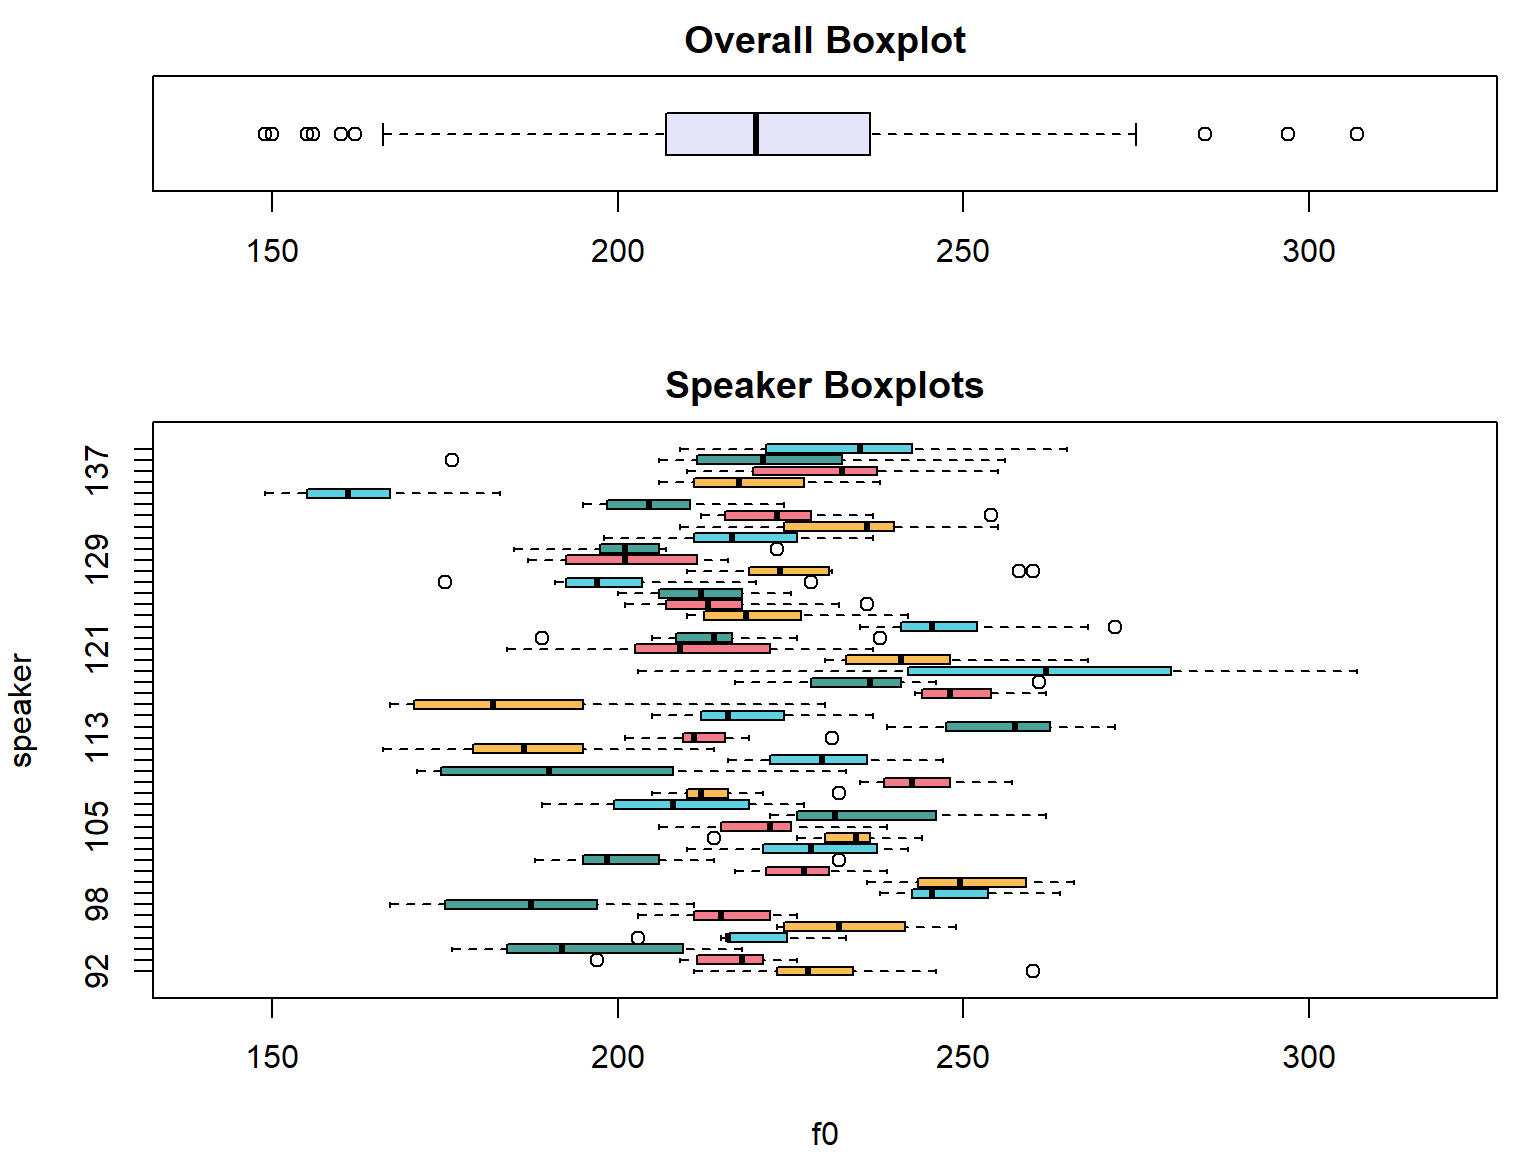
\includegraphics{02_files/figure-latex/F2-2-1.pdf}
\caption{\label{fig:F2-2}(top) Boxplot of overall distribution. (bottom) Speaker-specific boxplot of our f0 data.}
\end{figure}

\hypertarget{multilevel-models}{%
\subsection{Multilevel models}\label{multilevel-models}}

In linguistics (and many other similar fields) almost all of our data is repeated measures data. The methods most commonly-used by linguists (e.g., experiments, interviews, corpora, \ldots{} etc.) yield many observations per person, and typically all involve data from multiple people/sources. As a result, the analysis of this data requires that models be able to account for within \emph{and} between speaker variation in our data. Multilevel models address the correlated nature of repeated measures data by estimating multiple sources of variation simultaneously.

We can think about how this applies to our f0 sample. Each person picked at random has some average f0 they produce. This is \emph{between-speaker} variation: If you pick to people at random they will differ. However, each person also produces a different random f0 every time they speak, so that they will never produce exactly their average f0: this is \emph{within-speaker} variation.

Repeated-measures data leads to random variation in parameters that is \emph{indistinguishable} from that of our `data'. For example, consider the figure below. First we consider a single speaker's production (left) and produce a histogram that suggests a normal distribution reminiscent in shape to the overall aggregated data. In the middle, we see individual boxplots showing variation in speaker averages. Here we see that although each speakers productions are a distribution, variation in the distribution of the speaker averages is its own sort of distribution. Finally, on the right we see a histogram of the speaker averages and see that these are also normally distributed.

To a large extent, whether something is a parameter or a data point depends somewhat on your perspective. For example, consider the figure below. If you are trying to estimate a speaker's mean f0, then the individual productions might be `data' and the mean can be thought of as a `parameter'. If you were instead only interested in the population average, maybe now your subject mean is actually just a single data point, and the \emph{population} mean is actually your `parameter'.

\begin{figure}
\centering
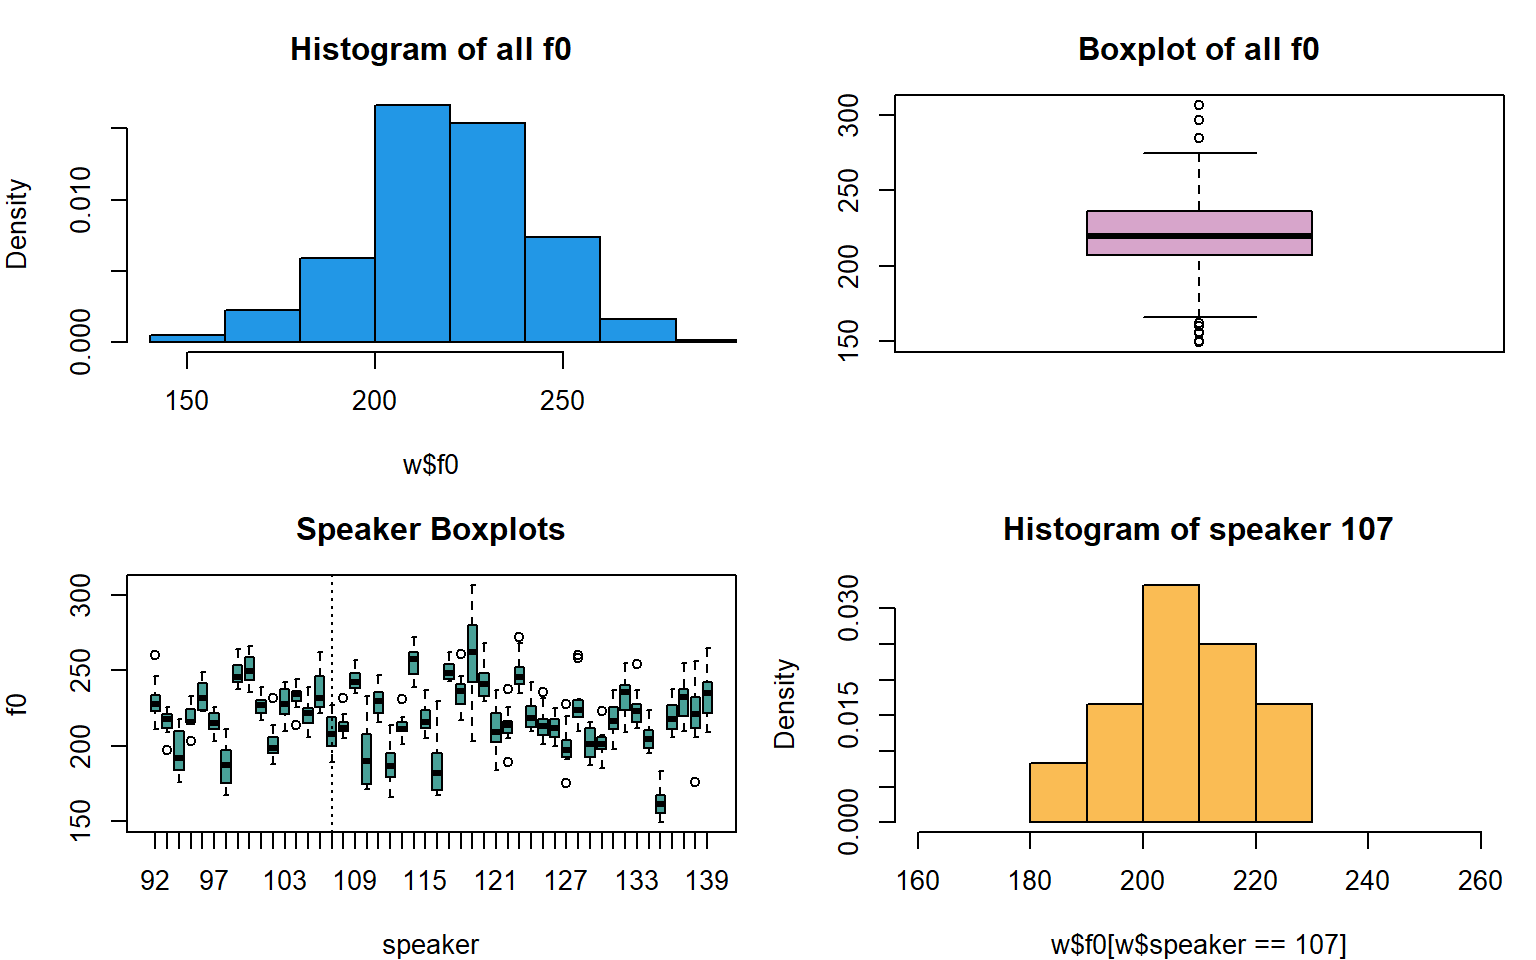
\includegraphics{02_files/figure-latex/F2-3-1.pdf}
\caption{\label{fig:F2-3}(top left) All the f0 data (top right) A boxplot of the same data. (bottom left) Speaker-specific boxplots, with a vertical line for speaker 107. (bottom right) The histogram of data produced by speaker 107.}
\end{figure}

A multilevel model is able to simultaneously estimate variation at multiple `levels'. This is actually why it's called a \emph{multilevel} model! For our f0 data, our `levels' are:

\begin{itemize}
\item
  The `upper' level: Between-speaker variation in mean f0. This can be thought of as variation in a new variable, which we will call \(\mu_{speaker}\). Speakers have an average f0 (\(\mu_{speaker}\)) that they produce over time. However, speakers are chosen randomly from a larger population, and so any given speaker's \(\mu_{speaker}\) is unpredictable a priori.
\item
  The `lower' level: Within-speaker variation, random error analogous to \(\varepsilon\). When an individual speaker produces speech, their productions will vary around their average from token to token. Our model cannot explain this and so this is `error'
\end{itemize}

As seen in the figure above, the variation at the lower and upper levels are analogous. Just like individual speakers will rarely have an average f0 exactly like the population average, individual speakers will rarely produce f0 values exactly at their speaker average. Importantly, variation at the two levels is independent and logically distinct: within-speaker variation can be small or large independently of whether between-speaker variation is large or small.

Basically, each subject's productions form a little normal distribution around their average, and the mix of these little distributions results in the overall `big' distribution of data across all subjects. By using multilevel models, we can estimate the effects of multiple sources of variation at the same time.

\hypertarget{estimating-a-multilevel-model-with-brms}{%
\section{\texorpdfstring{Estimating a multilevel model with \texttt{brms}}{Estimating a multilevel model with brms}}\label{estimating-a-multilevel-model-with-brms}}

We're now going to fit the same model we fit above, but with a structure that reflects the repeated-measures nature of the data. Whereas the last model was a pedagogical device, this model structure is actually appropriate to analyze this particular dataset.

\hypertarget{description-of-the-model-1}{%
\subsection{Description of the model}\label{description-of-the-model-1}}

We're going to keep working on developing an intuitive understanding for model notation, and using it to describe models. Just keep in mind that this is nothing more than an efficient way to denote the concepts being discussed in the text.

To specify a multilevel model, you need to write a slightly more complicated model formula. This explanation assumes that you have a dataframe or matrix where one column contains the variable you are interested in predicting (in this case \texttt{f0}), and another column contains a vector containing unique labels for each speaker/listener/participant (in this case a unique speaker label \texttt{speaker}).

To indicate that your model contains an `upper' level where you have clusters of data coming from different individuals, you have to put another model inside your main model!

Before, the model formula looked like this:

\texttt{f0\ \textasciitilde{}\ 1}

which meant `predict f0 using only an intercept'. Now the model formula will look like this:

\texttt{f0\ \textasciitilde{}\ 1\ +\ (\ 1\ \textbar{}\ speaker)}

When you place a predictor in the formula in parenthesis and on the right-hand-side of a pipe, like this \texttt{(\ \textbar{}\ predictor\ )}, you tell \texttt{brm} that you expect data to be clustered according to each category represented in the grouping vector. In this case, we are telling \texttt{brm} that each unique speaker is a cluster of data. Whatever you put in the left-hand-side of the parentheses \texttt{(\ in\ here\ \textbar{}\ predictor\ )} is the model for each subcluster!

So what does this model formula mean: \texttt{f0\ \textasciitilde{}\ 1\ +\ (\ 1\ \textbar{}\ speaker)}? Remember a model formula consisting only of a \texttt{1} tells \texttt{brm} that we have an Intercept-only model. So, our new formula tells \texttt{brm}: predict f0 based on only an overall intercept, but also estimate a different intercept for each speaker. Effectively, this model formula is telling \texttt{brm} to figure out all the information presented in the figures above.

This regression model is now something like this:

\begin{equation}
\begin{split}
\\
f0_{[i]} \sim \mathcal{N}(\mu_{[i]},\sigma) \\ \\
\mu_{[i]} = Intercept + \alpha_{speaker_{[i]}} \\
\\
\end{split}
\label{eq:26}
\end{equation}

In plain English, the model above says: we expect f0 to be normally distributed. The f0 value we expect for any given token is equal to some overall average (\(Intercept\)), and some value associated with the individual speaker (\(\alpha_{speaker_{[i]}}\)) who uttered the trial.

We now have another term \(\alpha_{speaker}\), in addition to the intercept. This coefficient is actually a set of coefficients since it has a different value for each speaker (it's a vector). Notice that the although the Intercept is fixed, value of \(\alpha_{speaker}\) that should be used will vary from trial to trial based on the speaker associated with the trial. We will discuss coefficients like these in more detail later, we don't really need to worry about it for now.

The value of \(\alpha_{speaker}\) has a different value for each speaker because it will reflect variation in \(\mu_{speaker}\), the average f0 value produced by each speaker. However, \(\mu_{speaker}\) is a random variable since it reflects the random average f0 of each person drawn from the population. If \(\mu_{speaker}\) behaves like a random variable, then the coefficients that reflect this value in our model (\(\alpha_{speaker}\)) will behave in the same way.

This means that our model actually has \emph{two} random variables. The first one is the error term \(\varepsilon_{[i]} \sim \mathcal{N}(0,\sigma_{error})\), which has a mean of 0 and a standard deviation which we can refer to as \(\sigma_{error}\). The second is the random coefficients that allow for speaker-specific adjustments to the intercept (\(\alpha_{speaker}\)). These can also be thought of as random draw from a normal distribution.

A careful consideration of the model in equation 2.4 suggests that the (\(\alpha_{speaker}\)) coefficients can't actually be exactly equal to \(\mu_{speaker}\), the average f0 for a speaker. If the overall mean (the intercept) is 220 Hz and a speaker's average is 230, this would suggest a predicted average of 450 (\(Intercept + \mu_{speaker}\)) for this speaker. Clearly that is not how the model should be working.

Recall that regression models encode \emph{differences}, rather than absolute values. Our model already represents the overall data average in the intercept parameter. Thus, the speaker-specific averages only need to contain information about \emph{differences} to this reference value. As a result, coefficients such as \(\alpha_{speaker}\) are modelled as being normally distributed with a mean of 0, and with some population-specific standard deviation.

Since our model coefficients reflect speaker-specific \emph{deviations} rather than the actual mean f0 of different speakers, people often use this symbol, \(\gamma\), for them instead of \(\mu\), where \(\gamma\) reflects the difference between the speaker means and the mean for the population of speakers, \(\gamma_{speaker} = \mu_{speaker} - \mu_{population}\).

We can show the expected distribution of this variable below, where \(\sigma_{speakers}\) is a population-specific standard deviation term. Note the similarity of this to the expected variation in our original data in Equation \eqref{eq:24}.

\begin{equation}
\begin{split}
\\
\gamma_{speaker} \sim \mathcal{N}(0,\sigma_{speakers}) \\ \\ 
\gamma_{speaker} = \alpha_{speaker} \\ \\
\end{split}
\label{eq:27}
\end{equation}

Our overall model is now as shown below, made specific for the data we have, and using expected parameter names.

\begin{equation}
\begin{split}
\\
f0_{[i]} \sim \mathcal{N}(\mu_{[i]},\sigma_{error}) \\ \\
\mu_{[i]} = Intercept + \alpha_{speaker_{[i]}} \\ \\
\alpha_{speaker} \sim \mathcal{N}(0,\sigma_{speakers}) \\ \\
\end{split}
\label{eq:28}
\end{equation}

Each line in the model says the following:

\begin{itemize}
\item
  observed f0 is expected to be normally distributed around a trial-specific mean, with some unknown but fixed standard deviation (\(\sigma_{error}\)).
\item
  the expected value for a given trial (\(\mu_{[i]}\)) is equal to the model intercept, plus some speaker-specific deviation/difference from the intercept for the speaker that produced that trial (\(\alpha_{speaker_{[i]}}\)).
\item
  the speaker effects (\(\alpha_{speaker}\)) are also drawn from a normal distribution with a mean of 0 and a standard deviation of \(\sigma_{speakers}\). This distribution represents the random, but systematic, between-speaker variation in average productions that exists within any population of speakers.
\end{itemize}

All of this information can be seen in the speaker boxplots below. The model intercept (horizontal dotted line) represents the overall mean, and the variation in \(\alpha_{speaker}\) is what causes the middle of each little box to differ from the mean. Finally, the error causes there to be a spread, a \emph{distribution}, around each speaker's individual mean.

\begin{figure}
\centering
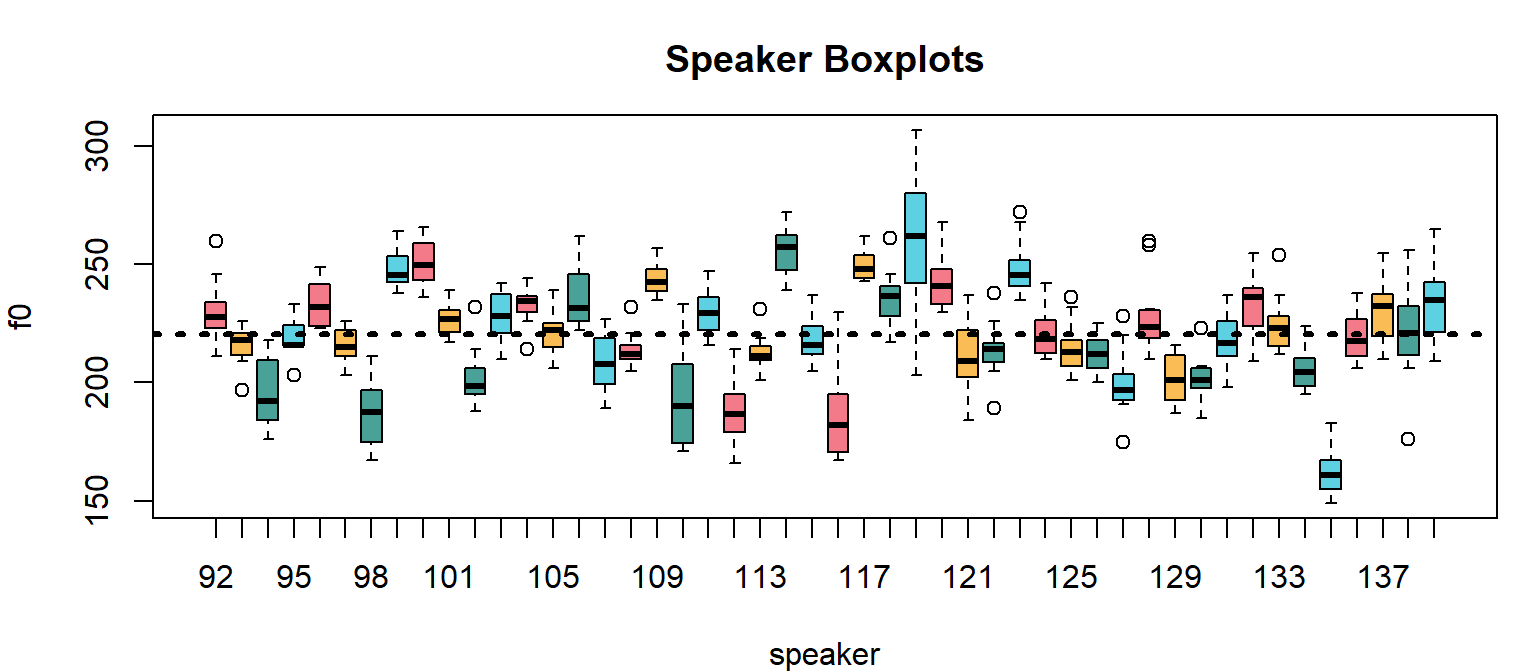
\includegraphics{02_files/figure-latex/F2-4-1.pdf}
\caption{\label{fig:F2-4}Speaker-specific boxplots for the f0 data.}
\end{figure}

There is a very important difference in how the first and second models we fit view and partition the variation in our model. The initial model we fit broke down the total variation in the model (\(\sigma_{total}\)) like this:

\[
\sigma_{total} = \sigma_{error}
\label{eq:29}
\]

In other words, all variation was error. We don't know why values vary from the mean. Our multilevel model views the variation in our data like this:

\[
\sigma_{total} = \sigma_{speaker} + \sigma_{error}
\label{eq:210}
\]

From the perspective of this model, only the variation \emph{within} a speaker's individual boxplot is error. The differences from box to box represent random (but systematic) between-speaker variation in f0.

\hypertarget{fitting-the-model}{%
\subsection{Fitting the model}\label{fitting-the-model}}

We can fit a model with a formula that appropriately specifies the clustering we expect in our data. As a result, this model can estimate both between- and within-speaker variability.

\begin{Shaded}
\begin{Highlighting}[]
\CommentTok{\# Fit the model yourself, or}
\FunctionTok{set.seed}\NormalTok{ (}\DecValTok{1}\NormalTok{)}
\NormalTok{multilevel\_model }\OtherTok{=}  
  \FunctionTok{brm}\NormalTok{ (f0 }\SpecialCharTok{\textasciitilde{}}\NormalTok{ (}\DecValTok{1}\SpecialCharTok{|}\NormalTok{speaker), }\AttributeTok{data =}\NormalTok{ w, }\AttributeTok{chains =} \DecValTok{1}\NormalTok{, }\AttributeTok{cores =} \DecValTok{1}\NormalTok{)}

\CommentTok{\# download pre{-}fit model from: }
\CommentTok{\# github.com/santiagobarreda/stats{-}class/tree/master/models}
\CommentTok{\# and load after placing in working directory}
\NormalTok{multilevel\_model }\OtherTok{=} \FunctionTok{readRDS}\NormalTok{ (}\StringTok{"2\_multilevel\_model.RDS"}\NormalTok{)}
\end{Highlighting}
\end{Shaded}

\begin{Shaded}
\begin{Highlighting}[]
\CommentTok{\# inspect model}
\NormalTok{multilevel\_model}
\DocumentationTok{\#\#  Family: gaussian }
\DocumentationTok{\#\#   Links: mu = identity; sigma = identity }
\DocumentationTok{\#\# Formula: f0 \textasciitilde{} (1 | uspeaker) }
\DocumentationTok{\#\#    Data: w (Number of observations: 576) }
\DocumentationTok{\#\# Samples: 1 chains, each with iter = 2000; warmup = 1000; thin = 1;}
\DocumentationTok{\#\#          total post{-}warmup samples = 1000}
\DocumentationTok{\#\# }
\DocumentationTok{\#\# Group{-}Level Effects: }
\DocumentationTok{\#\# \textasciitilde{}uspeaker (Number of levels: 48) }
\DocumentationTok{\#\#               Estimate Est.Error l{-}95\% CI u{-}95\% CI Rhat Bulk\_ESS Tail\_ESS}
\DocumentationTok{\#\# sd(Intercept)    20.19      2.10    16.65    25.06 1.00      135      192}
\DocumentationTok{\#\# }
\DocumentationTok{\#\# Population{-}Level Effects: }
\DocumentationTok{\#\#           Estimate Est.Error l{-}95\% CI u{-}95\% CI Rhat Bulk\_ESS Tail\_ESS}
\DocumentationTok{\#\# Intercept   220.39      3.10   214.49   226.13 1.03       51      108}
\DocumentationTok{\#\# }
\DocumentationTok{\#\# Family Specific Parameters: }
\DocumentationTok{\#\#       Estimate Est.Error l{-}95\% CI u{-}95\% CI Rhat Bulk\_ESS Tail\_ESS}
\DocumentationTok{\#\# sigma    12.54      0.39    11.83    13.34 1.01      400      700}
\DocumentationTok{\#\# }
\DocumentationTok{\#\# Samples were drawn using sampling(NUTS). For each parameter, Bulk\_ESS}
\DocumentationTok{\#\# and Tail\_ESS are effective sample size measures, and Rhat is the potential}
\DocumentationTok{\#\# scale reduction factor on split chains (at convergence, Rhat = 1).}
\end{Highlighting}
\end{Shaded}

This new model contains one new chunk its print statement. This section tells us about the standard deviation for the Intercept (\texttt{sd(Intercept)}) for the \texttt{\textasciitilde{}speaker} cluster:

\begin{Shaded}
\begin{Highlighting}[]
\DocumentationTok{\#\# Group{-}Level Effects: }
\DocumentationTok{\#\# \textasciitilde{}speaker (Number of levels: 48) }
\DocumentationTok{\#\#               Estimate Est.Error l{-}95\% CI u{-}95\% CI Rhat Bulk\_ESS Tail\_ESS}
\DocumentationTok{\#\# sd(Intercept)    20.19      2.10    16.65    25.06 1.00      135      192}
\end{Highlighting}
\end{Shaded}

This parameter corresponds to \(\sigma_{speaker}\) above, the standard deviation of between-speaker averages (\(\alpha_{speaker}\)) in the sample. Below, we calculate the speaker mean f0 values, the standard deviation of these, and the amount of within-speaker variation in f0s.

\begin{Shaded}
\begin{Highlighting}[]
\CommentTok{\# find mean f0 for each speaker}
\NormalTok{speaker\_means }\OtherTok{=} \FunctionTok{aggregate}\NormalTok{ (f0 }\SpecialCharTok{\textasciitilde{}}\NormalTok{ speaker, }\AttributeTok{data =}\NormalTok{ w, }\AttributeTok{FUN =}\NormalTok{ mean) }
\CommentTok{\# find the within speaker standard deviation This is the within{-}talker \textquotesingle{}error\textquotesingle{}.}
\NormalTok{speaker\_sigmas }\OtherTok{=} \FunctionTok{aggregate}\NormalTok{ (f0 }\SpecialCharTok{\textasciitilde{}}\NormalTok{ speaker, }\AttributeTok{data =}\NormalTok{ w, }\AttributeTok{FUN =}\NormalTok{ sd) }

\CommentTok{\# the mean of the speaker means corresponds to our overall mean estimate}
\FunctionTok{mean}\NormalTok{ (speaker\_means}\SpecialCharTok{$}\NormalTok{f0)}
\DocumentationTok{\#\# [1] 220.401}

\CommentTok{\# the standard deviation of the speaker means corresponds to \textquotesingle{}sd(Intercept)\textquotesingle{}, the }
\CommentTok{\# estimate of the standard deviation of speaker intercepts}
\FunctionTok{sd}\NormalTok{ (speaker\_means}\SpecialCharTok{$}\NormalTok{f0)}
\DocumentationTok{\#\# [1] 20.07397}

\CommentTok{\# the average within{-}speaker standard deviation corresponds to \textquotesingle{}sigma\textquotesingle{}, the }
\CommentTok{\# estimated error}
\FunctionTok{mean}\NormalTok{ (speaker\_sigmas}\SpecialCharTok{$}\NormalTok{f0)}
\DocumentationTok{\#\# [1] 11.6791}
\end{Highlighting}
\end{Shaded}

We are going to discuss the calculations we made above in terms of what they represent in the boxplots below. The overall mean f0 in our data (220.4) corresponds quite well to our model estimate of 220.4. This reflects the central location of the overall distribution below (the horizontal line in the figure below). The standard deviation of the speaker means (20.1) is again very similar to our model estimate (sd(Intercept) = 20.2). This reflects the average distance from each speaker's average to the overall average. Finally, the average of the within speaker standard deviation in our data (11.7) corresponds closely to our model's error estimate (sigma = 12.5). This reflects the average spread of each speaker's data relative to their own mean, within their own little boxplot. We can see that the information provided by \texttt{brms} is quite similar to what we can estimate directly using our data. However, \emph{brms} does this all for us, in addition to giving us a lot more information.

\begin{figure}
\centering
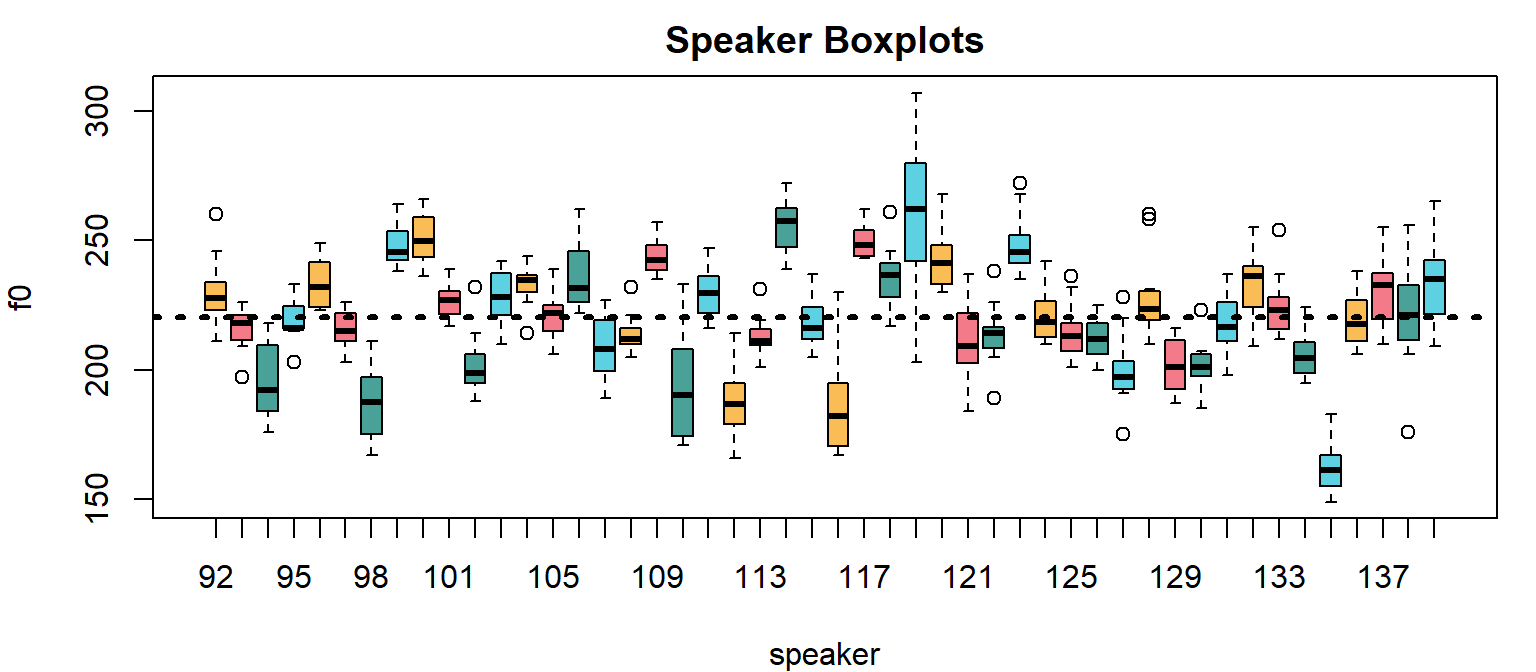
\includegraphics{02_files/figure-latex/F2-5-1.pdf}
\caption{\label{fig:F2-5}Speaker-specific boxplots for the f0 data we are analyzing.}
\end{figure}

\hypertarget{checking-model-convergence}{%
\section{Checking model convergence}\label{checking-model-convergence}}

Remember that our parameter estimates are based of a set of samples from the posterior distribution of a parameter. If we don't take enough of these samples, our parameter estimates will be unreliable.

For this reason, it's important to look at the ESS values (the `expected sample size'), and the `Rhat' values provided by \texttt{brm}. ESS tells you about how many independent samples you have taken from the likelihood. Bulk ESS is how many samples the sampler took in the thick part of the density, and Tail ESS reflects how much time the sampler spent in the thin part, the `tails'. Rhat tells you about whether your `chains' have converged (more on this later). As noted above, values of Rhat near 1 are good, and values higher than around 1.1 are a bad sign.

We haven't really taken many samples here, so we can't be confident in our parameter estimates. Ideally we would like several hundred samples (at least) for mean estimates, and thousands to be confident in the 95\% confidence intervals. If you fit a model and get a warning message like this:

\begin{Shaded}
\begin{Highlighting}[]
\DocumentationTok{\#\# Warning messages:}
\DocumentationTok{\#\# 1: Bulk Effective Samples Size (ESS) is too low, indicating posterior means and medians may be unreliable.}
\DocumentationTok{\#\# Running the chains for more iterations may help. See}
\DocumentationTok{\#\# http://mc{-}stan.org/misc/warnings.html\#bulk{-}ess}
\DocumentationTok{\#\# 2: Tail Effective Samples Size (ESS) is too low, indicating posterior variances and tail quantiles may be unreliable.}
\DocumentationTok{\#\# Running the chains for more iterations may help. See}
\DocumentationTok{\#\# http://mc{-}stan.org/misc/warnings.html\#tail{-}ess}
\end{Highlighting}
\end{Shaded}

That is \texttt{brms} telling you that you need to collect more samples in order to be confident in your parameter estimates. To get more samples we can run the model longer, or we can use more \emph{chains}. A chain is basically a separate set of samples for your parameter values. A model can be fit in parallel across several chains, and then the estimates can be merged across chains. When you do this across multiple cores, you can get N times as many samples when you use N cores. Since many computers these days have 4-8 (or more) cores, we can take advantage of parallel processing to fit models faster.

Before fitting a model across multiple cores, you should confirm how many you have. You can use the following command (you may need to install the \texttt{parallel} package):

\begin{Shaded}
\begin{Highlighting}[]
\NormalTok{parallel}\SpecialCharTok{::}\FunctionTok{detectCores}\NormalTok{()}
\end{Highlighting}
\end{Shaded}

I will be using four cores to fit models throughout. If you only have 4 total cores, consider changing the model fits to 2-3 chains and cores. One thing to keep in mind is that these models are computationally intensive to fit. As the datasets become larger and the models become more complicated, more powerful computers are needed in order to fit a model in a reasonable amount of time.

Below, I refit the same model from above but run it on 4 chains, and on 4 cores at once.

\begin{Shaded}
\begin{Highlighting}[]
\CommentTok{\# Fit the model yourself, or}
\FunctionTok{set.seed}\NormalTok{ (}\DecValTok{1}\NormalTok{)}
\NormalTok{multilevel\_multicore }\OtherTok{=}  
\NormalTok{  brms}\SpecialCharTok{::}\FunctionTok{brm}\NormalTok{ (f0 }\SpecialCharTok{\textasciitilde{}} \DecValTok{1} \SpecialCharTok{+}\NormalTok{ (}\DecValTok{1}\SpecialCharTok{|}\NormalTok{speaker), }\AttributeTok{data =}\NormalTok{ w, }\AttributeTok{chains =} \DecValTok{4}\NormalTok{, }\AttributeTok{cores =} \DecValTok{4}\NormalTok{)}

\CommentTok{\# download pre{-}fit model from: }
\CommentTok{\# github.com/santiagobarreda/stats{-}class/tree/master/models}
\CommentTok{\# and load after placing in working directory}
\NormalTok{multilevel\_multicore }\OtherTok{=} \FunctionTok{readRDS}\NormalTok{ (}\StringTok{\textquotesingle{}2\_multilevel\_multicore.RDS\textquotesingle{}}\NormalTok{)}
\end{Highlighting}
\end{Shaded}

\begin{Shaded}
\begin{Highlighting}[]
\CommentTok{\# inspect model}
\NormalTok{multilevel\_multicore}
\DocumentationTok{\#\#  Family: gaussian }
\DocumentationTok{\#\#   Links: mu = identity; sigma = identity }
\DocumentationTok{\#\# Formula: f0 \textasciitilde{} 1 + (1 | uspeaker) }
\DocumentationTok{\#\#    Data: w (Number of observations: 576) }
\DocumentationTok{\#\# Samples: 4 chains, each with iter = 2000; warmup = 1000; thin = 1;}
\DocumentationTok{\#\#          total post{-}warmup samples = 4000}
\DocumentationTok{\#\# }
\DocumentationTok{\#\# Group{-}Level Effects: }
\DocumentationTok{\#\# \textasciitilde{}uspeaker (Number of levels: 48) }
\DocumentationTok{\#\#               Estimate Est.Error l{-}95\% CI u{-}95\% CI Rhat Bulk\_ESS Tail\_ESS}
\DocumentationTok{\#\# sd(Intercept)    20.22      2.19    16.54    25.19 1.02      345      615}
\DocumentationTok{\#\# }
\DocumentationTok{\#\# Population{-}Level Effects: }
\DocumentationTok{\#\#           Estimate Est.Error l{-}95\% CI u{-}95\% CI Rhat Bulk\_ESS Tail\_ESS}
\DocumentationTok{\#\# Intercept   220.47      2.91   214.67   226.14 1.02      228      543}
\DocumentationTok{\#\# }
\DocumentationTok{\#\# Family Specific Parameters: }
\DocumentationTok{\#\#       Estimate Est.Error l{-}95\% CI u{-}95\% CI Rhat Bulk\_ESS Tail\_ESS}
\DocumentationTok{\#\# sigma    12.54      0.39    11.81    13.34 1.00     3427     2943}
\DocumentationTok{\#\# }
\DocumentationTok{\#\# Samples were drawn using sampling(NUTS). For each parameter, Bulk\_ESS}
\DocumentationTok{\#\# and Tail\_ESS are effective sample size measures, and Rhat is the potential}
\DocumentationTok{\#\# scale reduction factor on split chains (at convergence, Rhat = 1).}
\end{Highlighting}
\end{Shaded}

If we compare the ESS for this new model to the previous model, we see that using 4 chains has substantially increased our ESS, without taking up any more computing time.

One final tweak that I will be using going forward is to `thin' samples. Notice that we have collected \texttt{total\ post-warmup\ samples\ =\ 4000}. This means our model has 4000 samples for every parameter in the model. However, for some parameter we have only about 400 `effective samples'. This means that a lot of our samples are basically dead weight, taking up space and slowing down future computations for no good reason.

The discrepancy between the number of samples and the `effective' number of samples is due to something called \emph{autocorrelation}. Sometimes consecutive samples can be too similar and so don't given you that much \emph{independent} information. When this happens you end up with less information about a parameter than you might think based on the number of samples you have. One way to fix this is to run longer chains and keep only every Nth one. This lets your models be smaller while containing approximately the same information.

To do this you have to change the \texttt{iter}, \texttt{warmup} and \texttt{thin} parameters. You will keep every sample after the warmup is done, up to the \texttt{iter} maximum. So if \texttt{iter=3000} and \texttt{warmup=1000} you will end up with 2000 samples. After this, you keep only one every \texttt{thin} samples. Basically, you will end up with \((iter-warmup) / thin\) samples per chain. If you are doing this across \texttt{Ncores} cores, then you will end up with \(((iter-warmup) / thin) \times Ncores\) samples in total.

Below, I ask for 11,000 sample per chain. Since the warmup is 1000 this means we will keep 10,000 post warm-up. However, since \texttt{thin=10}, we will keep only 1000 of these. Finally, since we are fitting the model on four cores, we will end up with 4000 samples in total. As a resul, despite having the same number of samples as the \texttt{multilevel\_multicore}, the ESS for this model is much higher for important parameters such as the model intercept.

\begin{Shaded}
\begin{Highlighting}[]
\CommentTok{\# Fit the model yourself, or}
\FunctionTok{set.seed}\NormalTok{ (}\DecValTok{1}\NormalTok{)}
\NormalTok{multilevel\_thinned }\OtherTok{=}  
  \FunctionTok{brm}\NormalTok{ (f0 }\SpecialCharTok{\textasciitilde{}} \DecValTok{1} \SpecialCharTok{+}\NormalTok{ (}\DecValTok{1}\SpecialCharTok{|}\NormalTok{speaker), }\AttributeTok{data =}\NormalTok{ w, }\AttributeTok{chains =} \DecValTok{4}\NormalTok{, }\AttributeTok{cores =} \DecValTok{4}\NormalTok{,}
       \AttributeTok{warmup =} \DecValTok{1000}\NormalTok{, }\AttributeTok{iter =} \DecValTok{11000}\NormalTok{, }\AttributeTok{thin =} \DecValTok{10}\NormalTok{)}

\CommentTok{\# download pre{-}fit model from: }
\CommentTok{\# github.com/santiagobarreda/stats{-}class/tree/master/models}
\CommentTok{\# and load after placing in working directory}
\NormalTok{multilevel\_thinned }\OtherTok{=} \FunctionTok{readRDS}\NormalTok{ (}\StringTok{\textquotesingle{}2\_multilevel\_thinned.RDS\textquotesingle{}}\NormalTok{)}
\end{Highlighting}
\end{Shaded}

\begin{Shaded}
\begin{Highlighting}[]
\CommentTok{\# inspect model}
\NormalTok{multilevel\_thinned}
\DocumentationTok{\#\#  Family: gaussian }
\DocumentationTok{\#\#   Links: mu = identity; sigma = identity }
\DocumentationTok{\#\# Formula: f0 \textasciitilde{} 1 + (1 | uspeaker) }
\DocumentationTok{\#\#    Data: w (Number of observations: 576) }
\DocumentationTok{\#\# Samples: 4 chains, each with iter = 11000; warmup = 1000; thin = 10;}
\DocumentationTok{\#\#          total post{-}warmup samples = 4000}
\DocumentationTok{\#\# }
\DocumentationTok{\#\# Group{-}Level Effects: }
\DocumentationTok{\#\# \textasciitilde{}uspeaker (Number of levels: 48) }
\DocumentationTok{\#\#               Estimate Est.Error l{-}95\% CI u{-}95\% CI Rhat Bulk\_ESS Tail\_ESS}
\DocumentationTok{\#\# sd(Intercept)    20.06      2.23    16.24    24.98 1.00     2775     3392}
\DocumentationTok{\#\# }
\DocumentationTok{\#\# Population{-}Level Effects: }
\DocumentationTok{\#\#           Estimate Est.Error l{-}95\% CI u{-}95\% CI Rhat Bulk\_ESS Tail\_ESS}
\DocumentationTok{\#\# Intercept   220.40      2.95   214.57   226.19 1.00     1987     2625}
\DocumentationTok{\#\# }
\DocumentationTok{\#\# Family Specific Parameters: }
\DocumentationTok{\#\#       Estimate Est.Error l{-}95\% CI u{-}95\% CI Rhat Bulk\_ESS Tail\_ESS}
\DocumentationTok{\#\# sigma    12.54      0.38    11.81    13.31 1.00     3908     3891}
\DocumentationTok{\#\# }
\DocumentationTok{\#\# Samples were drawn using sampling(NUTS). For each parameter, Bulk\_ESS}
\DocumentationTok{\#\# and Tail\_ESS are effective sample size measures, and Rhat is the potential}
\DocumentationTok{\#\# scale reduction factor on split chains (at convergence, Rhat = 1).}
\end{Highlighting}
\end{Shaded}

\hypertarget{specifying-prior-probabilities}{%
\section{Specifying prior probabilities}\label{specifying-prior-probabilities}}

In Chapter 1 we discussed that Bayesian models require that prior probabilities be specified for all parameters. You may have noticed that to this point I haven't discussed priors at all.

If you don't specify prior probabilities for your parameters, \texttt{brm} will use a `flat/uniform' prior for all parameters. When you do this, you are basically relying only on the likelihood for your analysis. You are also telling your model that, a priori, \emph{any} value of average f0 is equally believable. Empirically, this is false. As a practical matter this can cause problems for samplers like STAN (which is what \texttt{brm} relies on). Basically, in the absence of proper priors the sampler has a harder time figuring out the most likely values when you tell it to look anywhere from positive to negative infinity. Even a bit of guidance can help.

\texttt{brms} makes it really easy to specify prior probabilities for specific parameters or whole groups of parameters. Below, I set priors for whole classes of parameters. In the example below, I use this information to set reasonable bounds on the parameters in the model. I do this by class of parameter:

\begin{itemize}
\tightlist
\item
  \texttt{Intercept}: this is a unique class, only for intercepts.
\item
  \texttt{b}: this is for all the non-intercept predictors. There are none in this model for now.
\item
  \texttt{sd}: this is for our standard deviation parameters that relate to `batches' of parameters. In our example this is \texttt{sd(Intercept)} for \texttt{speaker} (\(\sigma_{speakers}\)).
\item
  \texttt{sigma}: this is for any error parameters. Our only has one (but it could have more!), that is \texttt{sigma} (\(\sigma_{error}\)).
\end{itemize}

We're not going to worry about priors too much for now, and we're just going to set what are called `weakly informative' prior probabilities for our parameters. These are priors that encode a bit of information about our prior beliefes for a parameter, but are not \emph{too} strong. To set these, you have to use what you know about your variables, the world, and a healthy does of `common sense'. We will see a lot of examples of, and strategies for, setting priors in this book so you will get a chance to build your intuitions about it.

Both priors below use a `t' distribution, which is just like a normal distribution but it's more pointy, and has more density in the outer parts of the distribution. You can use normal priors, or any other priors that you think work for your model. Rather than focusing on the \emph{mathematical} properties of priors, the most important thing is that their \emph{shape} reflect the distribution of credible parameter values a priori (before you conducted your experiment).

The code to set the priors for our model looks like this:

\begin{Shaded}
\begin{Highlighting}[]
\NormalTok{  prior }\OtherTok{=} \FunctionTok{c}\NormalTok{(}\FunctionTok{set\_prior}\NormalTok{(}\StringTok{"student\_t(3, 220, 50)"}\NormalTok{, }\AttributeTok{class =} \StringTok{"Intercept"}\NormalTok{),}
            \FunctionTok{set\_prior}\NormalTok{(}\StringTok{"student\_t(3, 0, 100)"}\NormalTok{, }\AttributeTok{class =} \StringTok{"sd"}\NormalTok{),}
            \FunctionTok{set\_prior}\NormalTok{(}\StringTok{"student\_t(3, 0, 100)"}\NormalTok{, }\AttributeTok{class =} \StringTok{"sigma"}\NormalTok{))}
\end{Highlighting}
\end{Shaded}

The format for the priors is like this \texttt{student\_t(nu,\ mean,\ sd)}, where \texttt{nu} is a parameter that determines how pointy the distribution is, and \texttt{mean} and \texttt{sd} are the same mean and standard deviation parameters from the normal distribution. The nu parameter ranges from 1 to infinity, and large numbers result in a more normal-like distribution. We will talk about the t-distribution ins more detail later.

For the overall model intercept we set a prior probability of \texttt{student\_t(3,\ 220,\ 110)}. Around 90-95\% of the distribution of normal and t distributions is within two standard deviations of the mean. This means that I am saying the intercept should be between around 0 and 440 Hz. Since this range is higher than the range of human speaker f0s (about 80-300 Hz), this prior is not going to affect our outcomes very much.

The prior for the speaker standard deviation parameter (\(\sigma_{speakers}\)) is \texttt{student\_t(3,\ 0,\ 100)}, which specifies a t distribution centered at 0, with a standard deviation of 100. Since standard deviations can only be positive, the sampler (STAN) used by \texttt{brm} ignores the negative half, and uses only the positive values in the prior distribution. This prior just says that we expect the average difference between speakers to be less than 200 Hz (which it definitely is).

Finally, the prior for the random error is also \texttt{student\_t(3,\ 0,\ 100)}. Again, this says that we expect that the standard deviation of our random error to be less than 200 Hz. Since our random error is within-speaker variation, this is a again a massive overestimation of the likely magnitude of the random error in this data.

The left panel below compares the t distribution we used (blue) to the equivalent normal distribution (red). Although it may not seem like much of a difference, the t distribution can tolerate more extreme values because of its `fatter' (more dense) tails. As we will discuss later, using t distributions can make our models more robust to outliers. This is really important in linguistics where subjects/speakers sometimes do weird stuff! As we can see, the prior distribution we used for the intercept is much broader (more vague) than the data distribution so that it will have basically no effect on our results (but will help our model fit properly).

The right panel compares the prior for the standard deviation parameters to the absolute value of the centered f0 data. This presentation shows how far each observation is from the mean f0 (at 220 Hz). Obviously, people can't differ from each other by more than deviations differ from the mean. As a result, we see that the prior distribution we have assigned for the \texttt{sigma} (i.e., \(\sigma_{[speaker]}\)) and speaker \texttt{sd(Intercept)} parameter (i.e., \(\sigma_{[speaker]}\)) are much broader than these parameters could be, given the data. As a result, neither of these priors is going to have much of an effect on our parameter estimates.

\begin{figure}
\centering
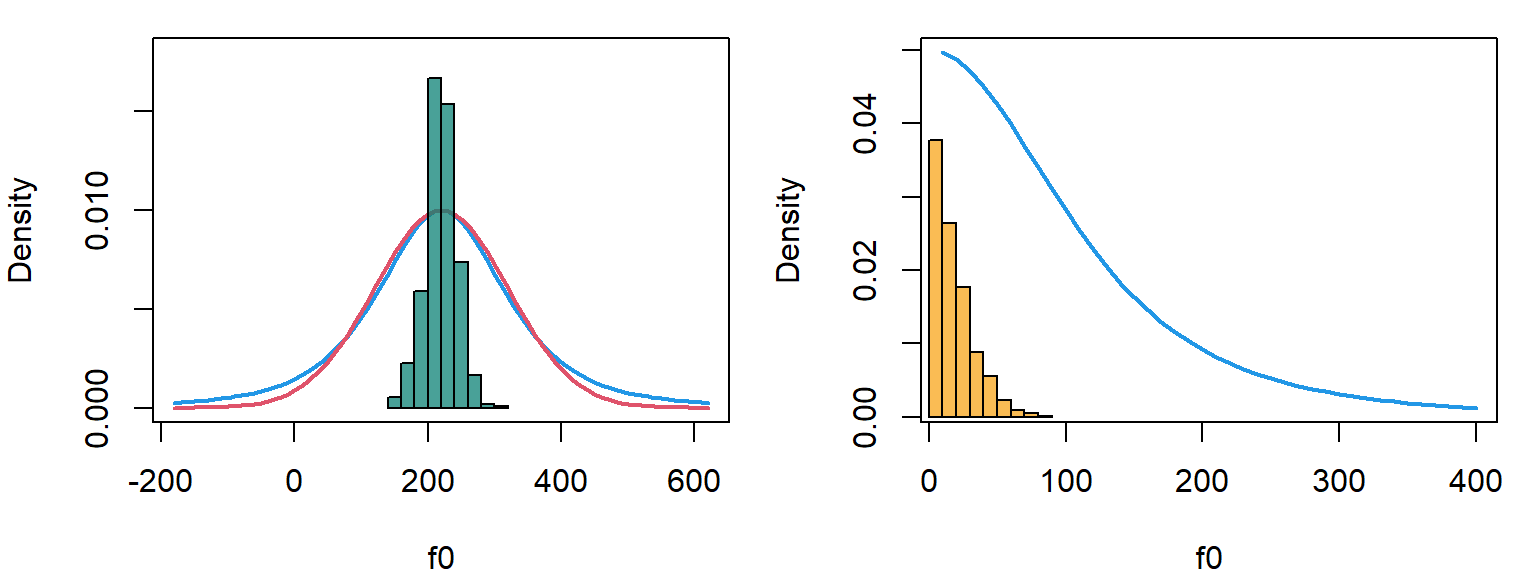
\includegraphics{02_files/figure-latex/F2-6-1.pdf}
\caption{\label{fig:F2-6}(left) A comparison of the densities of normal and t distributions with the same means and sigma parameters. The histogram shows our f0 data. (right) The distribution of absolute deviations from the mean for our f0 data, compared to the prior distributions of our standard deviation parameters in our model.}
\end{figure}

We can fit this new model below, and inspect the output. If we compare the output of this model to \texttt{multilevel\_thinned}, we see that specifying a prior has has no noticeable effect on our results. This is because the prior matters less and less when you have a lot of data, and because we have set wide priors that are appropriate (but vague) given our data. Although the priors may not matter much for models as simple as these, they can be very important when working with more complex data, and are a necessary component of Bayesian modeling.

\begin{Shaded}
\begin{Highlighting}[]
\CommentTok{\# Fit the model yourself, or}
\FunctionTok{set.seed}\NormalTok{ (}\DecValTok{1}\NormalTok{)}
\NormalTok{multilevel\_priors }\OtherTok{=}  
  \FunctionTok{brm}\NormalTok{ (f0 }\SpecialCharTok{\textasciitilde{}} \DecValTok{1} \SpecialCharTok{+}\NormalTok{ (}\DecValTok{1}\SpecialCharTok{|}\NormalTok{speaker), }\AttributeTok{data =}\NormalTok{ w, }\AttributeTok{chains =} \DecValTok{4}\NormalTok{, }\AttributeTok{cores =} \DecValTok{4}\NormalTok{,}
       \AttributeTok{warmup =} \DecValTok{1000}\NormalTok{, }\AttributeTok{iter =} \DecValTok{11000}\NormalTok{, }\AttributeTok{thin =} \DecValTok{10}\NormalTok{,}
       \AttributeTok{prior =} \FunctionTok{c}\NormalTok{(}\FunctionTok{set\_prior}\NormalTok{(}\StringTok{"student\_t(3, 220, 100)"}\NormalTok{, }\AttributeTok{class =} \StringTok{"Intercept"}\NormalTok{),}
                 \FunctionTok{set\_prior}\NormalTok{(}\StringTok{"student\_t(3, 0, 100)"}\NormalTok{, }\AttributeTok{class =} \StringTok{"sd"}\NormalTok{),}
                 \FunctionTok{set\_prior}\NormalTok{(}\StringTok{"student\_t(3, 0, 100)"}\NormalTok{, }\AttributeTok{class =} \StringTok{"sigma"}\NormalTok{)))}

\CommentTok{\# download pre{-}fit model from: }
\CommentTok{\# github.com/santiagobarreda/stats{-}class/tree/master/models}
\CommentTok{\# and load after placing in working directory}
\NormalTok{multilevel\_priors }\OtherTok{=} \FunctionTok{readRDS}\NormalTok{ (}\StringTok{\textquotesingle{}2\_multilevel\_priors.RDS\textquotesingle{}}\NormalTok{)}
\end{Highlighting}
\end{Shaded}

\begin{Shaded}
\begin{Highlighting}[]
\CommentTok{\# inspect model}
\NormalTok{multilevel\_priors}
\DocumentationTok{\#\#  Family: gaussian }
\DocumentationTok{\#\#   Links: mu = identity; sigma = identity }
\DocumentationTok{\#\# Formula: f0 \textasciitilde{} 1 + (1 | uspeaker) }
\DocumentationTok{\#\#    Data: w (Number of observations: 576) }
\DocumentationTok{\#\# Samples: 4 chains, each with iter = 11000; warmup = 1000; thin = 10;}
\DocumentationTok{\#\#          total post{-}warmup samples = 4000}
\DocumentationTok{\#\# }
\DocumentationTok{\#\# Group{-}Level Effects: }
\DocumentationTok{\#\# \textasciitilde{}uspeaker (Number of levels: 48) }
\DocumentationTok{\#\#               Estimate Est.Error l{-}95\% CI u{-}95\% CI Rhat Bulk\_ESS Tail\_ESS}
\DocumentationTok{\#\# sd(Intercept)    20.19      2.24    16.29    25.06 1.00     3114     3663}
\DocumentationTok{\#\# }
\DocumentationTok{\#\# Population{-}Level Effects: }
\DocumentationTok{\#\#           Estimate Est.Error l{-}95\% CI u{-}95\% CI Rhat Bulk\_ESS Tail\_ESS}
\DocumentationTok{\#\# Intercept   220.42      2.97   214.44   226.38 1.00     1796     2841}
\DocumentationTok{\#\# }
\DocumentationTok{\#\# Family Specific Parameters: }
\DocumentationTok{\#\#       Estimate Est.Error l{-}95\% CI u{-}95\% CI Rhat Bulk\_ESS Tail\_ESS}
\DocumentationTok{\#\# sigma    12.54      0.39    11.81    13.34 1.00     3968     3972}
\DocumentationTok{\#\# }
\DocumentationTok{\#\# Samples were drawn using sampling(NUTS). For each parameter, Bulk\_ESS}
\DocumentationTok{\#\# and Tail\_ESS are effective sample size measures, and Rhat is the potential}
\DocumentationTok{\#\# scale reduction factor on split chains (at convergence, Rhat = 1).}
\end{Highlighting}
\end{Shaded}

\hypertarget{answering-our-research-questions}{%
\section{Answering our research questions}\label{answering-our-research-questions}}

Let's return to the research questions we posed initially in Chapoter 1, and again at the beginning of this chapter:

\begin{enumerate}
\def\labelenumi{\arabic{enumi})}
\item
  What is the average f0 of the whole \emph{population} likely to be?
\item
  Can we set bounds on likely mean f0 values based on the data we collected?
\end{enumerate}

And we can compare the answers provided to this question by our initial model (which contained no priors or information about repeated measured) and final models (which contained information about speakers and appropriate priors).

\begin{Shaded}
\begin{Highlighting}[]
\NormalTok{model}
\DocumentationTok{\#\#  Family: gaussian }
\DocumentationTok{\#\#   Links: mu = identity; sigma = identity }
\DocumentationTok{\#\# Formula: f0 \textasciitilde{} 1 }
\DocumentationTok{\#\#    Data: w (Number of observations: 576) }
\DocumentationTok{\#\# Samples: 1 chains, each with iter = 2000; warmup = 1000; thin = 1;}
\DocumentationTok{\#\#          total post{-}warmup samples = 1000}
\DocumentationTok{\#\# }
\DocumentationTok{\#\# Population{-}Level Effects: }
\DocumentationTok{\#\#           Estimate Est.Error l{-}95\% CI u{-}95\% CI Rhat Bulk\_ESS Tail\_ESS}
\DocumentationTok{\#\# Intercept   220.40      0.97   218.33   222.30 1.00      851      557}
\DocumentationTok{\#\# }
\DocumentationTok{\#\# Family Specific Parameters: }
\DocumentationTok{\#\#       Estimate Est.Error l{-}95\% CI u{-}95\% CI Rhat Bulk\_ESS Tail\_ESS}
\DocumentationTok{\#\# sigma    23.24      0.69    21.99    24.61 1.00      653      550}
\DocumentationTok{\#\# }
\DocumentationTok{\#\# Samples were drawn using sampling(NUTS). For each parameter, Bulk\_ESS}
\DocumentationTok{\#\# and Tail\_ESS are effective sample size measures, and Rhat is the potential}
\DocumentationTok{\#\# scale reduction factor on split chains (at convergence, Rhat = 1).}

\NormalTok{multilevel\_priors}
\DocumentationTok{\#\#  Family: gaussian }
\DocumentationTok{\#\#   Links: mu = identity; sigma = identity }
\DocumentationTok{\#\# Formula: f0 \textasciitilde{} 1 + (1 | uspeaker) }
\DocumentationTok{\#\#    Data: w (Number of observations: 576) }
\DocumentationTok{\#\# Samples: 4 chains, each with iter = 11000; warmup = 1000; thin = 10;}
\DocumentationTok{\#\#          total post{-}warmup samples = 4000}
\DocumentationTok{\#\# }
\DocumentationTok{\#\# Group{-}Level Effects: }
\DocumentationTok{\#\# \textasciitilde{}uspeaker (Number of levels: 48) }
\DocumentationTok{\#\#               Estimate Est.Error l{-}95\% CI u{-}95\% CI Rhat Bulk\_ESS Tail\_ESS}
\DocumentationTok{\#\# sd(Intercept)    20.19      2.24    16.29    25.06 1.00     3114     3663}
\DocumentationTok{\#\# }
\DocumentationTok{\#\# Population{-}Level Effects: }
\DocumentationTok{\#\#           Estimate Est.Error l{-}95\% CI u{-}95\% CI Rhat Bulk\_ESS Tail\_ESS}
\DocumentationTok{\#\# Intercept   220.42      2.97   214.44   226.38 1.00     1796     2841}
\DocumentationTok{\#\# }
\DocumentationTok{\#\# Family Specific Parameters: }
\DocumentationTok{\#\#       Estimate Est.Error l{-}95\% CI u{-}95\% CI Rhat Bulk\_ESS Tail\_ESS}
\DocumentationTok{\#\# sigma    12.54      0.39    11.81    13.34 1.00     3968     3972}
\DocumentationTok{\#\# }
\DocumentationTok{\#\# Samples were drawn using sampling(NUTS). For each parameter, Bulk\_ESS}
\DocumentationTok{\#\# and Tail\_ESS are effective sample size measures, and Rhat is the potential}
\DocumentationTok{\#\# scale reduction factor on split chains (at convergence, Rhat = 1).}
\end{Highlighting}
\end{Shaded}

Our initial model (\texttt{model}) and our final model (\texttt{multilevel\_priors}) agree on what the average f0 is. However, they disagree on a credible interval for that parameter. Our initial model did not specify information about repeated measures. This causes our model to think that it has more independent observations than it does, and so it returns an overly-precise estimate.

Another difference is that the final model has a much smaller \texttt{sigma} parameter (12.5 vs 23.2). This indicates that the error (\(\varepsilon\)) is much smaller in the final model than in the initial model. Keep in mind that `error' is just what your model can't explain. Our final model explains much more and so there is less error. The reduced error is a direct consequence of the fact that the final model splits the variation in the data into between-speaker and within-speaker components (i.e., \(\sigma_{total}=\sigma_{speaker}+\sigma_{error}\)), estimating the between-speaker variation (\(\sigma_{speaker}\)) to be about 20 Hz. Since \(\sigma_{total}\) is a fixed value (given the data), obviously the larger your between-speaker variation is (\(\sigma_{speaker}\)), the smaller your random error ((\(\sigma_{error}\))) \emph{must} be.

Usually, when I report parameters I provide the mean and standard deviations of the posterior distribution, in addition to the bounds of the 95\% credible interval of the parameter. Based on the result of our final model, I think a thorough description of the general properties of our data might go something like:

\begin{quote}
"Based on our model the average f0 produced by adult females in Michigan is likely to be 220 Hz (s.d. = 2.97, 95\% CI = 214.4, 226.4). However, consistent between-speaker variation averages about 20 Hz (s.d. = 2.24, 95\% CI = 16.29, 25.06), meaning that we can expect the average f0 produced by individuals to deviate substantially from 220 Hz. Finally, the standard deviation of production error was about 12.5 Hz (s.d. = 0.39, 95\% CI = 11.81, 13.34) indicating that the amount of random within-speaker variation in production is about half the magnitude of the systematic between-speaker differences in f0.
\end{quote}

I'm again including the speaker boxplots below because I think this image basically presents the same information as the paragraph above, but in visual form. In general, any data relationship or result can be presented in a figure, and the relationships presented in a figure can also be expressed as a mathematical model.

When you are thinking about the relationships in your data, or that you expect in your data, its a good idea to think: what kind of picture could illustrate this relationship? Conversely, if you see a figure of your results that you feel really expresses something interesting about your data you should think, how can these relationships be represented in a model?

\begin{figure}
\centering
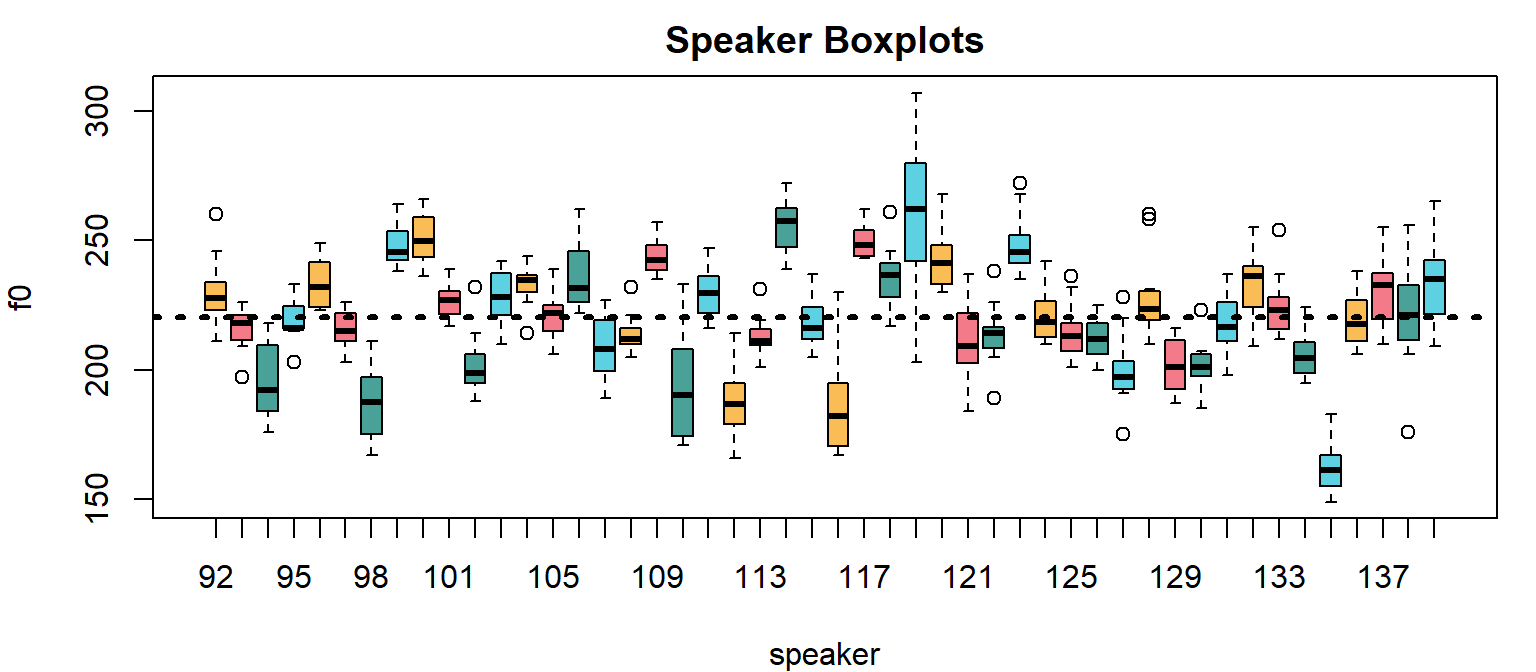
\includegraphics{02_files/figure-latex/F2-7-1.pdf}
\caption{\label{fig:F2-7}Speaker-specific boxplots for the f0 data.}
\end{figure}

\hypertarget{simulating-data-using-our-model-parameters}{%
\section{Simulating data using our model parameters}\label{simulating-data-using-our-model-parameters}}

One way to think about what all these numbers mean is to simulate data that has the same characteristics, and build fake data from the individual component parts. The code chunk below does exactly this for the data we have been discussing thus far.

First, there is an intercept equal to 220.4 Hz. Then, I create effects representing 48 simulated `female talkers' from a population just like our observed population. These effects are stored in a vector called \texttt{alpha\_speaker}, and they represent the values of \(\alpha_{speaker}\) for our different speakers. These speaker effects come from a population with a mean of 0 and a standard deviation (\(\sigma_{speaker}\)) equal to 20.4 (like our data). Each of these simulated speakers produces 12 productions, and so we need a \texttt{speakers} vector with values that repeat 12 times each to index the \texttt{alpha\_speaker} vector containing the effects.

I also draw our error, \(\varepsilon\). This error comes from a distribution with a mean of 0 and a standard deviation equal to \(\sigma_{error}\). It's important to note that the error is just 48x12 random draws from this population. There is no distinction between one person's productions and another when it comes to the error. If there were, this would indicate differences in sigma between speakers! Our model assumes a single error population for all speakers (but it doesn't \emph{have} to be this way).

\begin{Shaded}
\begin{Highlighting}[]
\DocumentationTok{\#\# don\textquotesingle{}t run this line if you want a new simulated dataset. }
\FunctionTok{set.seed}\NormalTok{(}\DecValTok{5}\NormalTok{)}
\DocumentationTok{\#\# this is the value of our intercept}
\NormalTok{Intercept }\OtherTok{=} \FloatTok{220.4}
\DocumentationTok{\#\# this is a vector of 48 speaker effects}
\NormalTok{alpha\_speaker }\OtherTok{=} \FunctionTok{rnorm}\NormalTok{ (}\DecValTok{48}\NormalTok{, }\DecValTok{0}\NormalTok{, }\FloatTok{20.2}\NormalTok{)}
\DocumentationTok{\#\# this is a vector indicating which speaker produced which utterance}
\NormalTok{speaker }\OtherTok{=} \FunctionTok{rep}\NormalTok{ (}\DecValTok{1}\SpecialCharTok{:}\DecValTok{48}\NormalTok{, }\AttributeTok{each =} \DecValTok{12}\NormalTok{)}
\DocumentationTok{\#\# this vector contains the error}
\NormalTok{epsilon }\OtherTok{=} \FunctionTok{rnorm}\NormalTok{ (}\DecValTok{48} \SpecialCharTok{*} \DecValTok{12}\NormalTok{, }\DecValTok{0}\NormalTok{, }\FloatTok{12.5}\NormalTok{)}
\end{Highlighting}
\end{Shaded}

After creating our components, we add the Intercept, speaker deflections and random error to make our fake `replicated' data. Since this data has the same statistical properties as our real data, it should look a lot like it.

\begin{Shaded}
\begin{Highlighting}[]
\CommentTok{\# the sum of an intercept, speaker deflections and random error makes our fake data}
\NormalTok{f0\_rep }\OtherTok{=}\NormalTok{ Intercept }\SpecialCharTok{+}\NormalTok{ alpha\_speaker[speaker] }\SpecialCharTok{+}\NormalTok{ epsilon}
\end{Highlighting}
\end{Shaded}

Below I compare the results of our simulation to our real data. If you didn't have a clear impression of what the data looked like, I doubt you could tell which is the real data. This tells us our model is a good reflection of the data!

\begin{figure}
\centering
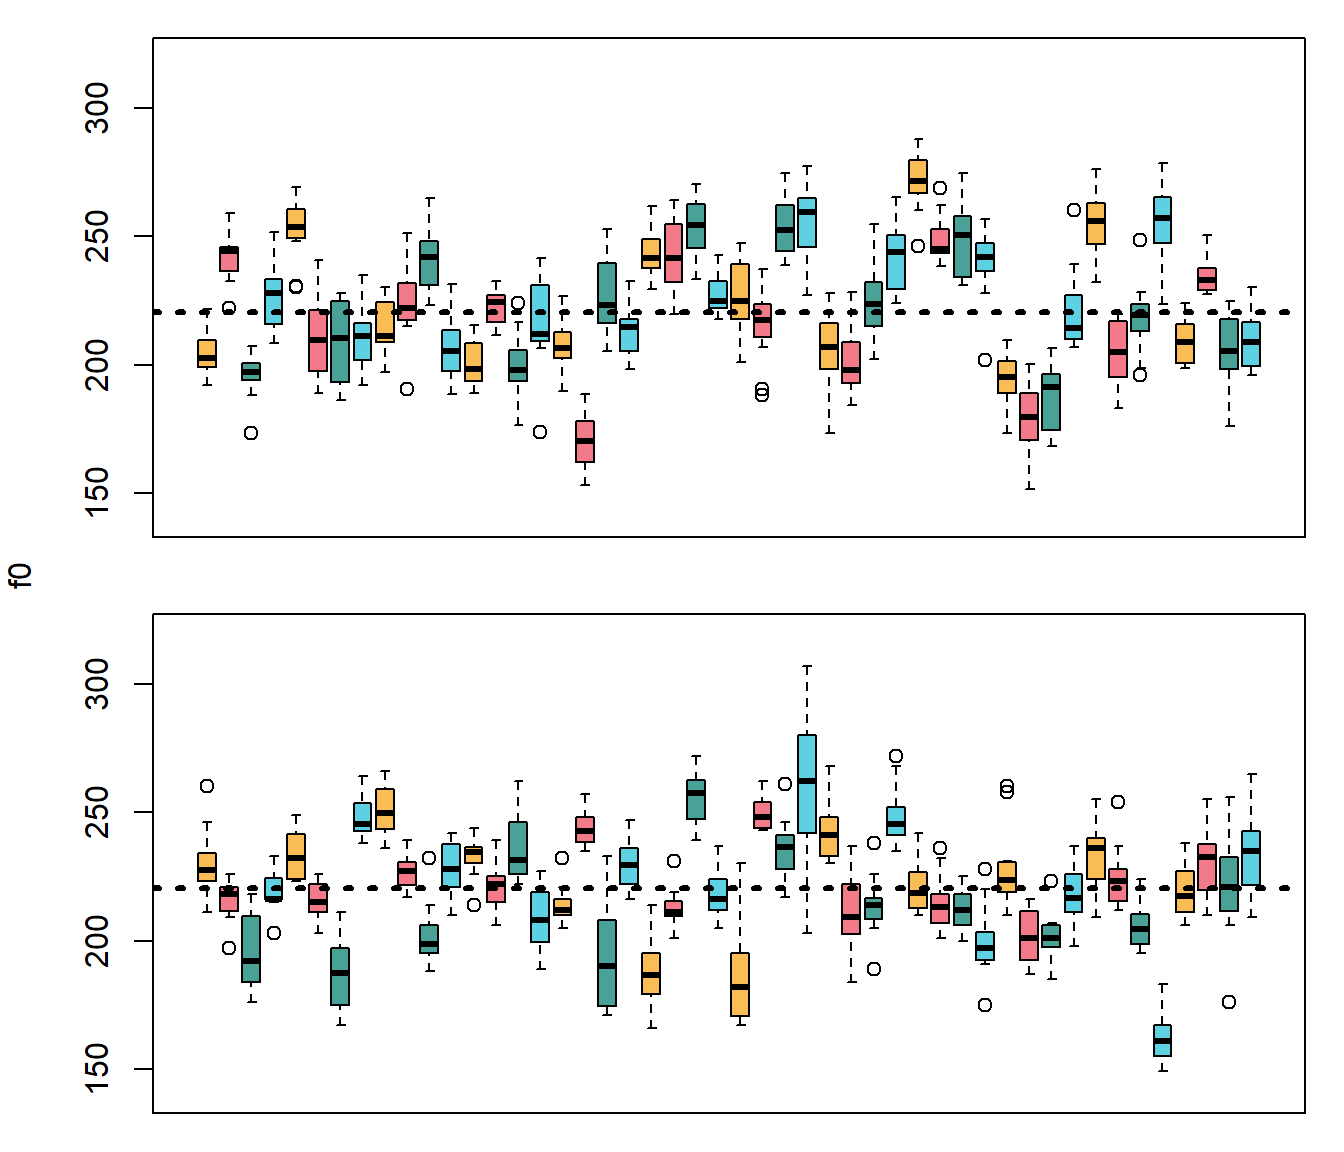
\includegraphics{02_files/figure-latex/F2-8-1.pdf}
\caption{\label{fig:F2-8}Comparison of real and simulated f0 production data.}
\end{figure}

Below I make two datasets that are `incomplete' with respect to the variation in our data. The first contains the intercept and noise only, the second contains the intercept and speaker effects only.

\begin{Shaded}
\begin{Highlighting}[]
\CommentTok{\# this fake data is missing between speaker variation}
\NormalTok{f0\_rep\_1 }\OtherTok{=}\NormalTok{ Intercept }\SpecialCharTok{+}\NormalTok{ epsilon}

\CommentTok{\# this fake data is missing within speaker variation}
\NormalTok{f0\_rep\_2 }\OtherTok{=}\NormalTok{ Intercept }\SpecialCharTok{+}\NormalTok{ alpha\_speaker[speaker]}
\end{Highlighting}
\end{Shaded}

In the figure below, I compare these `incomplete' datasets to the full simulated data. The top row contains only error (\(\varepsilon, \sigma_{error}\)). As a result, f0 varies around the intercept, but there is no speaker to speaker variation. This is what that data would look like if there is no random variation in means across subjects.

However, notice that each little box is not centered at 0. Although the error distribution is centered at 0, the small number of errors added to the speaker mean are \textbf{extremely} unlikely to add up to exactly 0. So, error contributes some unknown amount to each speaker's apparent average. This makes estimations of the \emph{real} speaker effects impossible in practice.

In the middle plot, the figure shows only between-speaker variation (\(\alpha_{speaker}, \sigma_{speaker}\)) but no within-speaker variation (i.e., no noise/error). Now we see that speakers vary from the intercept, but this representation does not show the fact that speakers also vary relative to their own average.

The final plot is the combination of the variation in the top two figures. The final plot shows the simulated data: the sum of the intercept, the within speaker variation and the between-speaker variation reflected in the values of the speaker intercepts.

\begin{figure}

{\centering 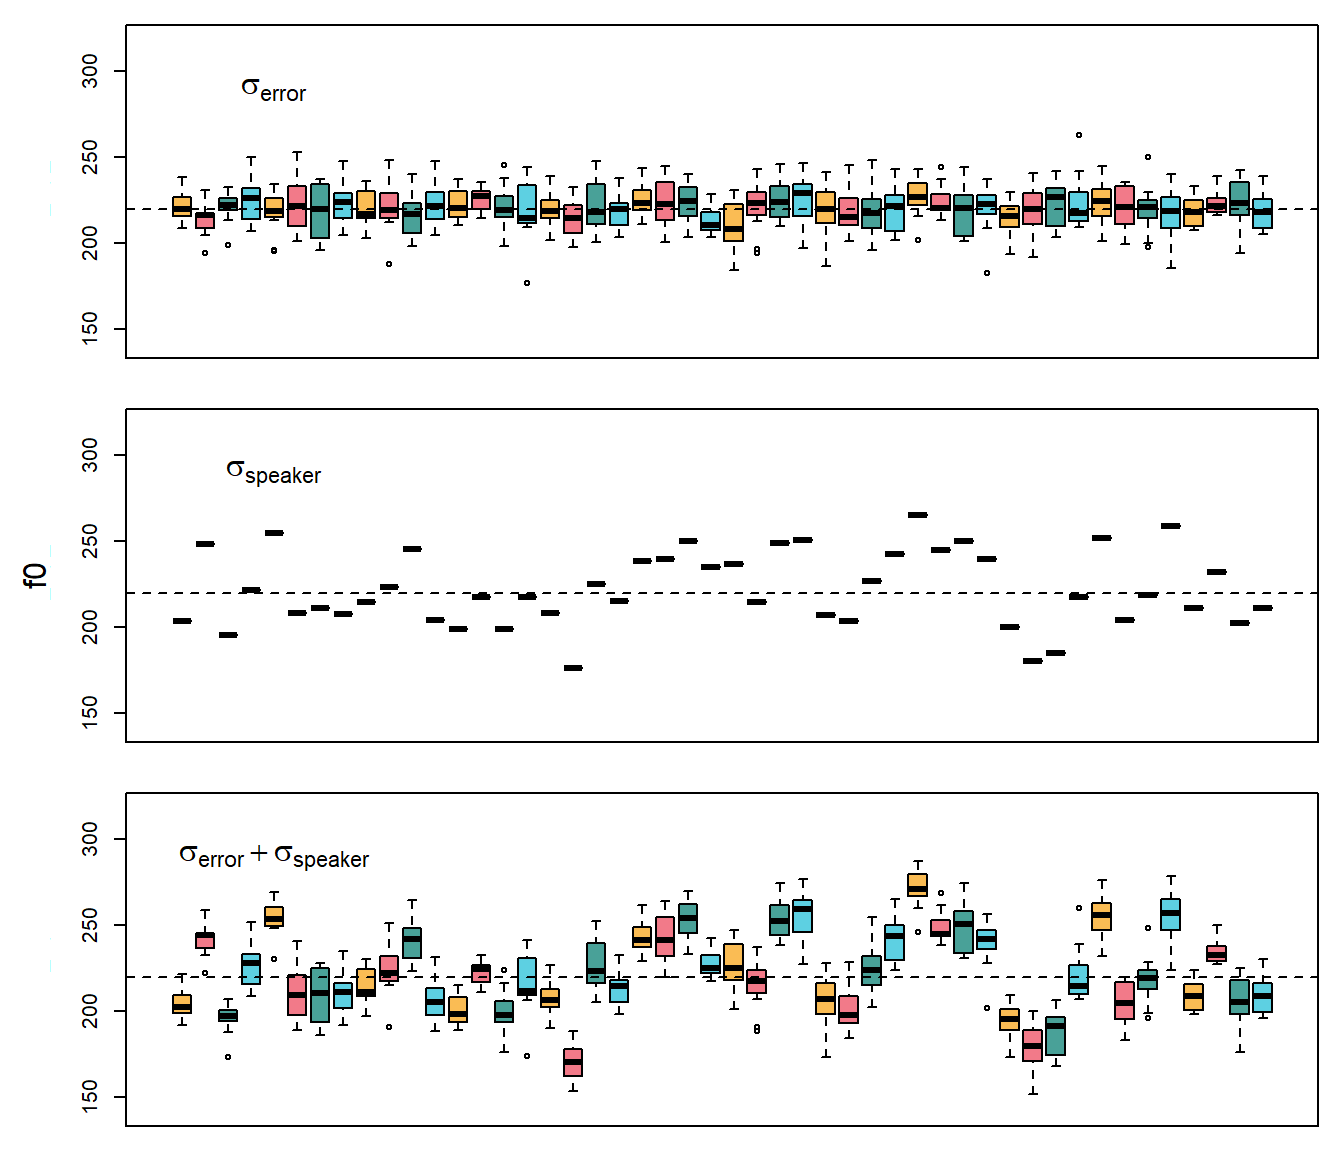
\includegraphics{02_files/figure-latex/F2-9-1} 

}

\caption{(top) Simulated error variation around the intercept. (middle) Simulated between-speaker variation, but no production error. (bottom) Simulated data containing both within and between-speaker variation in f0.}\label{fig:F2-9}
\end{figure}

\hypertarget{frequentist-corner}{%
\section{Frequentist corner}\label{frequentist-corner}}

We're going to compare the output of \texttt{brms} to some more `traditional' approaches. I'm not going to talk about the traditional models in any detail, the focus of this section is simply to highlight the similarities between different approaches, and to point out where to find equivalent information in the different models. As a result, this section will mostly be useful for people familiar with the traditional approaches.

\hypertarget{bayesian-multilevel-modesl-vs.-lmer}{%
\subsection{Bayesian multilevel modesl vs.~lmer}\label{bayesian-multilevel-modesl-vs.-lmer}}

First, we will compare the output of our multilevel Bayesian modesl to the output of the \texttt{lmer} (``linear mixed-effects regression'') function, a very popular function for fitting multilevel models in the \texttt{lme4} R package.

Below we fit a model just like our \texttt{multilevel\_priors} model. Note that the model syntax is identical and that, actually, the whole function call is quite similar to how we would fit the model using \texttt{brm}. This is a good thing, it means that much of the material we use in this book can also be used to work with the \texttt{lmer} function, should you find this more convenient.

\begin{Shaded}
\begin{Highlighting}[]
\FunctionTok{library}\NormalTok{ (lme4)}

\FunctionTok{set.seed}\NormalTok{ (}\DecValTok{1}\NormalTok{)}
\NormalTok{lmer\_model }\OtherTok{=} \FunctionTok{lmer}\NormalTok{ (f0 }\SpecialCharTok{\textasciitilde{}}\NormalTok{ (}\DecValTok{1}\SpecialCharTok{|}\NormalTok{speaker), }\AttributeTok{data =}\NormalTok{ w)}
\end{Highlighting}
\end{Shaded}

Below I've annotated the print statements for the equivalent \texttt{lmer} and \texttt{brm} models, and provide explanations for each section below.

\begin{Shaded}
\begin{Highlighting}[]
\CommentTok{\# print model summary}
\FunctionTok{summary}\NormalTok{ (lmer\_model)}

\DocumentationTok{\#\# (1) Linear mixed model fit by REML [\textquotesingle{}lmerMod\textquotesingle{}]}
\DocumentationTok{\#\# (1) Formula: f0 \textasciitilde{} (1 | speaker)}
\DocumentationTok{\#\# (1) Data: w}
\DocumentationTok{\#\# (1) }
\DocumentationTok{\#\# (1) REML criterion at convergence: 4705.8}
\DocumentationTok{\#\# (1)}
\DocumentationTok{\#\# (1) Scaled residuals: }
\DocumentationTok{\#\# (1)     Min      1Q  Median      3Q     Max }
\DocumentationTok{\#\# (1) {-}4.3792 {-}0.5962 {-}0.1005  0.4771  3.9273 }
\DocumentationTok{\#\#  }
\DocumentationTok{\#\#     Random effects:}
\DocumentationTok{\#\#      Groups   Name        Variance Std.Dev.}
\DocumentationTok{\#\# (2)  speaker  (Intercept) 389.9    19.75   }
\DocumentationTok{\#\# (3)  Residual             156.8    12.52   }
\DocumentationTok{\#\#     Number of obs: 576, groups:  speaker, 48}
\DocumentationTok{\#\#  }
\DocumentationTok{\#\#     Fixed effects:}
\DocumentationTok{\#\#                 Estimate Std. Error t value}
\DocumentationTok{\#\# (4) (Intercept)  220.401      2.897   76.07}
\end{Highlighting}
\end{Shaded}

\begin{Shaded}
\begin{Highlighting}[]
\NormalTok{multilevel\_priors}

\DocumentationTok{\#\# (1)  Family: gaussian }
\DocumentationTok{\#\# (1)   Links: mu = identity; sigma = identity }
\DocumentationTok{\#\# (1) Formula: f0 \textasciitilde{} 1 + (1 | speaker) }
\DocumentationTok{\#\# (1)    Data: w (Number of observations: 576) }
\DocumentationTok{\#\# (1) Samples: 4 chains, each with iter = 11000; warmup = 1000; thin = 10;}
\DocumentationTok{\#\# (1)          total post{-}warmup samples = 4000}
\DocumentationTok{\#\#  }
\DocumentationTok{\#\#     Group{-}Level Effects: }
\DocumentationTok{\#\# (2) \textasciitilde{}speaker (Number of levels: 48) }
\DocumentationTok{\#\# (2)               Estimate Est.Error l{-}95\% CI u{-}95\% CI Rhat Bulk\_ESS Tail\_ESS}
\DocumentationTok{\#\# (2) sd(Intercept)    20.32      2.23    16.44    25.32 1.00     2777     3254}
\DocumentationTok{\#\#  }
\DocumentationTok{\#\#     Population{-}Level Effects: }
\DocumentationTok{\#\#               Estimate Est.Error l{-}95\% CI u{-}95\% CI Rhat Bulk\_ESS Tail\_ESS}
\DocumentationTok{\#\# (4) Intercept   220.38      3.00   214.55   226.18 1.00     1639     2497}
\DocumentationTok{\#\#  }
\DocumentationTok{\#\# (3) Family Specific Parameters: }
\DocumentationTok{\#\# (3)        Estimate Est.Error l{-}95\% CI u{-}95\% CI Rhat Bulk\_ESS Tail\_ESS}
\DocumentationTok{\#\# (3) sigma    12.55      0.38    11.83    13.32 1.00     3963     3892}
\DocumentationTok{\#\# }
\DocumentationTok{\#\# (5) Samples were drawn using sampling(NUTS). For each parameter, Bulk\_ESS}
\DocumentationTok{\#\# (5) and Tail\_ESS are effective sample size measures, and Rhat is the potential}
\DocumentationTok{\#\# (5) scale reduction factor on split chains (at convergence, Rhat = 1).}
\end{Highlighting}
\end{Shaded}

Section (1) contains basic information about data and model structure, and is unique to each function. Generally, you won't pay much attention to this section when you use either function, but it does contain useful basic information about your model.

Section (2) in the \texttt{lmer} output presents the variance (389.9) and standard deviation (19.75) of the speaker effects (\(\alpha_{[speaker]}\)). Notice that in the equivalent section, \texttt{brm} gives you a mean (20.32) of a very similar values. However, unlike \texttt{lmer} which only returns what are called `point estimates', \texttt{brm} also gives you a credible interval around this parameter estimate. So, only \texttt{brm} tells you about a range of believable values, in addition to telling you the \emph{most} believable value.

Section (3) in \texttt{lmer} presents the variance (156.8) and standard deviation (12.52) of the \texttt{Residual}, which is what is calls the random error. In section (2) in the \texttt{brms} output we that the error is called \texttt{sigma}, although the estimate is about the same (12.55). Just as with the between-speaker variation about, \texttt{brm} returns an interval for this parameter while \texttt{lmer} returns only a point estimate.

In section (4) \texttt{lmer} and \texttt{brm} presents the model intercept. We see that the \texttt{Std.\ Error} estimate provided by \texttt{lmer} (2.897) corresponds closely to the standard deviation of the posterior distribution of the intercept parameter provided by \texttt{brm} (3.00). In addition, \texttt{brm} provides an interval around the intercept whereas \texttt{lmer} does not. Finally, in section (5) \texttt{brm} presnts some boilerplate that will look almost the same every time you fit a model.

In general, we see that \texttt{lmer} provides a subset of the information provided by \texttt{brm}, and that the two approaches provide basically the same values for estimates. This is because in both cases, results are being dominated by the likelihoods of different parameters. Although iit is to be expectem it is still reassuring, we woulnd't want there to be huge differences in our results just by being `Bayesian'.

\hypertarget{bayesian-multilevel-modesl-vs.-the-one-sample-t-test}{%
\subsection{Bayesian multilevel modesl vs.~the one-sample t-test}\label{bayesian-multilevel-modesl-vs.-the-one-sample-t-test}}

We can fit a one-sample t-test to our f0 vector.

\begin{Shaded}
\begin{Highlighting}[]
\FunctionTok{t.test}\NormalTok{ (w}\SpecialCharTok{$}\NormalTok{f0)}
\end{Highlighting}
\end{Shaded}

\begin{verbatim}
## 
##  One Sample t-test
## 
## data:  w$f0
## t = 227.8, df = 575, p-value < 2.2e-16
## alternative hypothesis: true mean is not equal to 0
## 95 percent confidence interval:
##  218.5007 222.3014
## sample estimates:
## mean of x 
##   220.401
\end{verbatim}

This usage is incorrect however, since this test requires that all the observations be independent from each other. Since we have 12 samples per speaker, these are not independent of each other. Notice however that the interval provided around the mean (\texttt{95\ percent\ confidence\ interval:\ 218.5007\ 222.3014}) corresponds very well to the interval around the intercept provided by our initial model above (\texttt{218.33\ \ \ 222.30}). The reason they align so well is because they both (inappropriately) treated all our observations as independent.

Below we use the one-sample t-test appropriately. We find the average for each speaker, and then use only those 48 values in our test.

\begin{Shaded}
\begin{Highlighting}[]
\NormalTok{speaker\_means }\OtherTok{=} \FunctionTok{aggregate}\NormalTok{ (f0 }\SpecialCharTok{\textasciitilde{}}\NormalTok{ speaker, }\AttributeTok{data =}\NormalTok{ w, }\AttributeTok{FUN =}\NormalTok{ mean) }
\FunctionTok{t.test}\NormalTok{ (speaker\_means}\SpecialCharTok{$}\NormalTok{f0)}
\end{Highlighting}
\end{Shaded}

\begin{verbatim}
## 
##  One Sample t-test
## 
## data:  speaker_means$f0
## t = 76.068, df = 47, p-value < 2.2e-16
## alternative hypothesis: true mean is not equal to 0
## 95 percent confidence interval:
##  214.5722 226.2299
## sample estimates:
## mean of x 
##   220.401
\end{verbatim}

Now the interval provided closely resembles that of our final, \texttt{multilevel\_priors} model (\texttt{214.55\ \ \ 226.18}). So, if all we care about is estimating a mean and credible interval around the mean, then a one-sample t-test will help us do that. However, our \texttt{multilevel\_priors} clearly provides us with substantially more information than is returned by the t-test.

\hypertarget{exercises-1}{%
\section{Exercises}\label{exercises-1}}

\begin{enumerate}
\def\labelenumi{\arabic{enumi})}
\item
  Use the code below to fit the final model we considered to the f0s produced by another group of speakers. See if you can get all of the same information out of the model that we considered above. Make a plot of this new data using the plot code provided.
\item
  See if you can use the information from your new data to update the simulated data created above. This entails finding the intercept, within-speaker, and between-speaker variation estimates in your new data and using this to generate a new batch of fake/replicated data.
\item
  Use the code below to fit the model below to your own data. Remember, this data should come from a single group of speakers/participants who each produce one or more data points. You will need to change \texttt{f0} and \texttt{speaker} in the model below to match the names of the columns containing this information in your data. You may also need to change the priors based on the ranges of your variables. If in doubt, you can just set all the priors to have means of 0 and standard deviations of 10,000 for now.
\end{enumerate}

\begin{Shaded}
\begin{Highlighting}[]
\CommentTok{\# Get data from course website}
\NormalTok{url1 }\OtherTok{=} \StringTok{"https://raw.githubusercontent.com/santiagobarreda"}
\NormalTok{url2 }\OtherTok{=} \StringTok{"/stats{-}class/master/data/h95\_vowel\_data.csv"}
\NormalTok{h95 }\OtherTok{=} \FunctionTok{read.csv}\NormalTok{ (}\FunctionTok{url}\NormalTok{(}\FunctionTok{paste0}\NormalTok{ (url1, url2)))}

\CommentTok{\# uncomment only one of the options below}

\CommentTok{\# select women only}
\CommentTok{\# f0\_data = h95[h95$group == \textquotesingle{}w\textquotesingle{},]}

\CommentTok{\# select boys only}
\CommentTok{\# f0\_data = h95[h95$group == \textquotesingle{}b\textquotesingle{},]}

\CommentTok{\# select girls only}
\CommentTok{\# f0\_data = h95[h95$group == \textquotesingle{}g\textquotesingle{},]}

\CommentTok{\# select men only}
\CommentTok{\# f0\_data = h95[h95$group == \textquotesingle{}m\textquotesingle{},]}

\NormalTok{exercise\_model }\OtherTok{=}  
  \FunctionTok{brm}\NormalTok{ (f0 }\SpecialCharTok{\textasciitilde{}} \DecValTok{1} \SpecialCharTok{+}\NormalTok{ (}\DecValTok{1}\SpecialCharTok{|}\NormalTok{speaker), }\AttributeTok{data =}\NormalTok{ f0\_data, }\AttributeTok{chains =} \DecValTok{4}\NormalTok{, }\AttributeTok{cores =} \DecValTok{4}\NormalTok{,}
       \AttributeTok{warmup =} \DecValTok{1000}\NormalTok{, }\AttributeTok{iter =} \DecValTok{11000}\NormalTok{, }\AttributeTok{thin =} \DecValTok{10}\NormalTok{,}
       \AttributeTok{prior =} \FunctionTok{c}\NormalTok{(}\FunctionTok{set\_prior}\NormalTok{(}\StringTok{"student\_t(3, 220, 100)"}\NormalTok{, }\AttributeTok{class =} \StringTok{"Intercept"}\NormalTok{),}
                 \FunctionTok{set\_prior}\NormalTok{(}\StringTok{"student\_t(3, 0, 100)"}\NormalTok{, }\AttributeTok{class =} \StringTok{"sd"}\NormalTok{),}
                 \FunctionTok{set\_prior}\NormalTok{(}\StringTok{"student\_t(3, 0, 100)"}\NormalTok{, }\AttributeTok{class =} \StringTok{"sigma"}\NormalTok{)))}
\end{Highlighting}
\end{Shaded}

\begin{Shaded}
\begin{Highlighting}[]
\NormalTok{url1 }\OtherTok{=} \StringTok{"https://raw.githubusercontent.com/santiagobarreda"}
\NormalTok{url2 }\OtherTok{=} \StringTok{"/stats{-}class/master/data/h95\_vowel\_data.csv"}
\CommentTok{\# set up colors for plotting}
\NormalTok{devtools}\SpecialCharTok{::}\FunctionTok{source\_url}\NormalTok{ (}\FunctionTok{paste0}\NormalTok{ (url1, }\StringTok{"/stats{-}class/master/data/colors.R"}\NormalTok{))}
\CommentTok{\# source functions}
\NormalTok{devtools}\SpecialCharTok{::}\FunctionTok{source\_url}\NormalTok{ (}\FunctionTok{paste0}\NormalTok{ (url1, }\StringTok{"/stats{-}class/master/data/functions.R"}\NormalTok{))}

\NormalTok{url1 }\OtherTok{=} \StringTok{"https://raw.githubusercontent.com/santiagobarreda/stats{-}class/master/data/"}
\NormalTok{h95 }\OtherTok{=} \FunctionTok{read.csv}\NormalTok{ (}\FunctionTok{url}\NormalTok{(}\FunctionTok{paste0}\NormalTok{ (url1, }\StringTok{"03\_h95\_vowel\_data.csv"}\NormalTok{)))}
\NormalTok{females }\OtherTok{=} \FunctionTok{read.csv}\NormalTok{ (}\FunctionTok{url}\NormalTok{(}\FunctionTok{paste0}\NormalTok{ (url1, }\StringTok{"03\_h95\_vowel\_data\_females.csv"}\NormalTok{)))}
\NormalTok{males }\OtherTok{=} \FunctionTok{read.csv}\NormalTok{ (}\FunctionTok{url}\NormalTok{(}\FunctionTok{paste0}\NormalTok{ (url1, }\StringTok{"03\_h95\_vowel\_data\_males.csv"}\NormalTok{)))}
\end{Highlighting}
\end{Shaded}

\hypertarget{comparing-two-groups-of-observations}{%
\chapter{Comparing two groups of observations}\label{comparing-two-groups-of-observations}}

In the previous chapter we focused on investigating values from a single group, which is basically the simplest kind data you can deal with. In this chapter we're going to compare data from two groups to see how similar/different they really are.

The models discussed in this chapter can be used for data that compares observations across two groups. We are using the term `groups' loosely here. The designs in this chapter are appropriate for data from:

\begin{itemize}
\item
  two groups of speakers/listeners that are grouped in different ways because they differ in some characteristic (e.g., gender), or in some experimental condition. Different speakers are in each group.
\item
  the same speakers/listeners are tested in two different experimental condition, with stimuli that vary in two groups, or something of the sort.
\item
  each speaker/subject can contribute multiple data points, and the number does not need to be balanced across subjects. Also speakers can be missing from one of the conditions (i.e., unbalanced data is ok).
\end{itemize}

The models we will discuss are similar to two-sample t-tests in the types of research questions they can help investigate (as will be discussed at the end of the chapter).

\hypertarget{data-and-research-questions-2}{%
\section{Data and research questions}\label{data-and-research-questions-2}}

We're going to use the Hillenbrand et al.~f0 data we used in the other chapters. Previously we only considered the productions of adult females from Michigan, this time we're going to compare the f0 measurements for adult females to those of girls between 10-12 years of age.

\begin{Shaded}
\begin{Highlighting}[]
\CommentTok{\# load brms}
\FunctionTok{library}\NormalTok{ (brms)}
\end{Highlighting}
\end{Shaded}

\begin{verbatim}
## Loading required package: Rcpp
\end{verbatim}

\begin{verbatim}
## Loading 'brms' package (version 2.15.0). Useful instructions
## can be found by typing help('brms'). A more detailed introduction
## to the package is available through vignette('brms_overview').
\end{verbatim}

\begin{verbatim}
## 
## Attaching package: 'brms'
\end{verbatim}

\begin{verbatim}
## The following object is masked from 'package:stats':
## 
##     ar
\end{verbatim}

\begin{Shaded}
\begin{Highlighting}[]
\CommentTok{\# get the data from the course website}
\NormalTok{url1 }\OtherTok{=} \StringTok{"https://raw.githubusercontent.com/santiagobarreda/stats{-}class/master/data/"}
\NormalTok{females }\OtherTok{=} \FunctionTok{read.csv}\NormalTok{ (}\FunctionTok{url}\NormalTok{(}\FunctionTok{paste0}\NormalTok{ (url1, }\StringTok{"03\_h95\_vowel\_data\_females.csv"}\NormalTok{)))}
\end{Highlighting}
\end{Shaded}

To be perfectly honest you won't really use single-group designs very much in your work. Research questions in linguistics most often require linguists to compare at least two conditions or groups of data. In a sense, even a single-group question carries an implicit comparison within it. Caring that the value of some variable is one value sort of presupposes that there is some other potential values of interest that is it not. What I mean by this is that simply saying ``the mean f0 produced by adult women from Michigan is 220 Hz'' indicates that the mean is \emph{not} 200 Hz, and it is \emph{not} 240 Hz, and thereby makes at least an implicit comparison.

In this chapter we will directly ask: Are two groups of observations different or are they the same? This kind of question comes up all the time in linguistic research. For example in phonetics, researchers ask questions like, have these vowels merged in this dialect (are these two things different)? Does visual information speed up speech perception or not (are two sets of reaction times the same)?

A good way to isolate a single difference is to create groups that differ primarily according to the characteristic you are interested in testing, but are otherwise the same `on average'. For the reaction-time example above, I might present the same listeners with very similar words in the same conditions, but where half of the words are presented with and half are presented without visual information. Any difference in reaction times between the groups should reflect the advantage provided by visual information. The question would then be, are reaction times with visual information \emph{the same thing} as reaction times without visual information? Are these two sets of observations groups sampled from the same population? Or is the set of observations ``reaction times for speech recognized \emph{with} visual information'' a different set of things than ``reaction times for speech recognized \emph{without} visual information''?

In our data we have male and female talkers of the same dialect, who differ primarily in terms of age. Basically, these groups differ mostly in terms of `adultness', and so we can use the characteristics of these groups to investigate the effect of `adultness' on average f0. Below I present boxplots that highlight the effect of adultness on f0, first overall and then divided by speaker gender.

\begin{figure}
\centering
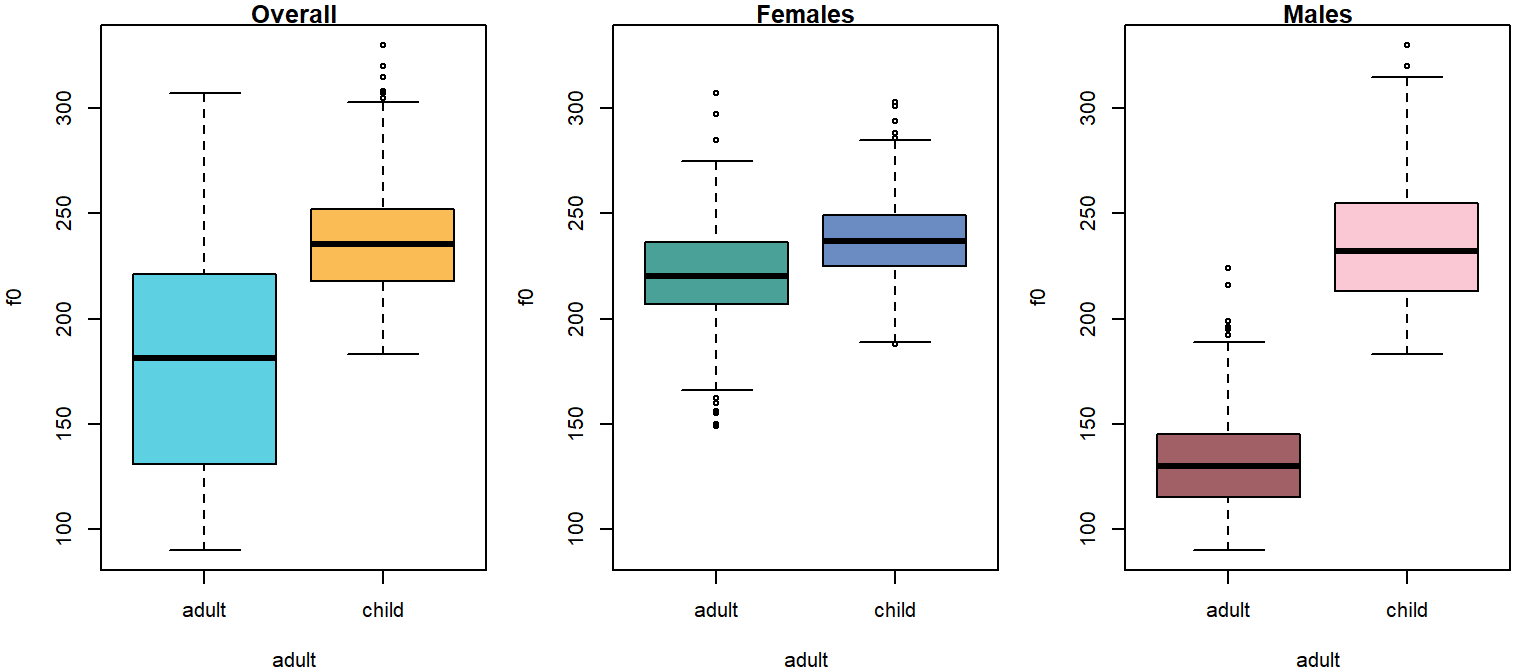
\includegraphics{03_files/figure-latex/F3-boxplots-1.pdf}
\caption{\label{fig:F3-boxplots}Boxplots comparing productions of f0 for different groupings of talkers.}
\end{figure}

Clearly there is a difference in f0 between children and adults, but the difference also seems to be gender-dependent: there is more of a difference between men and boys than between women and girls. We are going to focus on the female data for now, and the comparison of men and boys is left as an exercise.

Figure \ref{fig:F3-boxplots-density} highlights: between-speaker variation, within-speaker variation, and between-group variation. Obviously the distributions seem a \emph{bit} different, but they are also not \emph{that} different. We can also clearly see that there is substantial overlap between individual girls and women (in the figure on the left). Clearly neither ``they are totally the same'' nor ``they are totally different'' seems like it is supported by the data. As a result, a cautious analysis of this data will recognize the between-category overlap even if somehow the categories are found to be `different'. We're going to fit a model that can help us quantify all of the variability shown in the figures below.

\begin{figure}
\centering
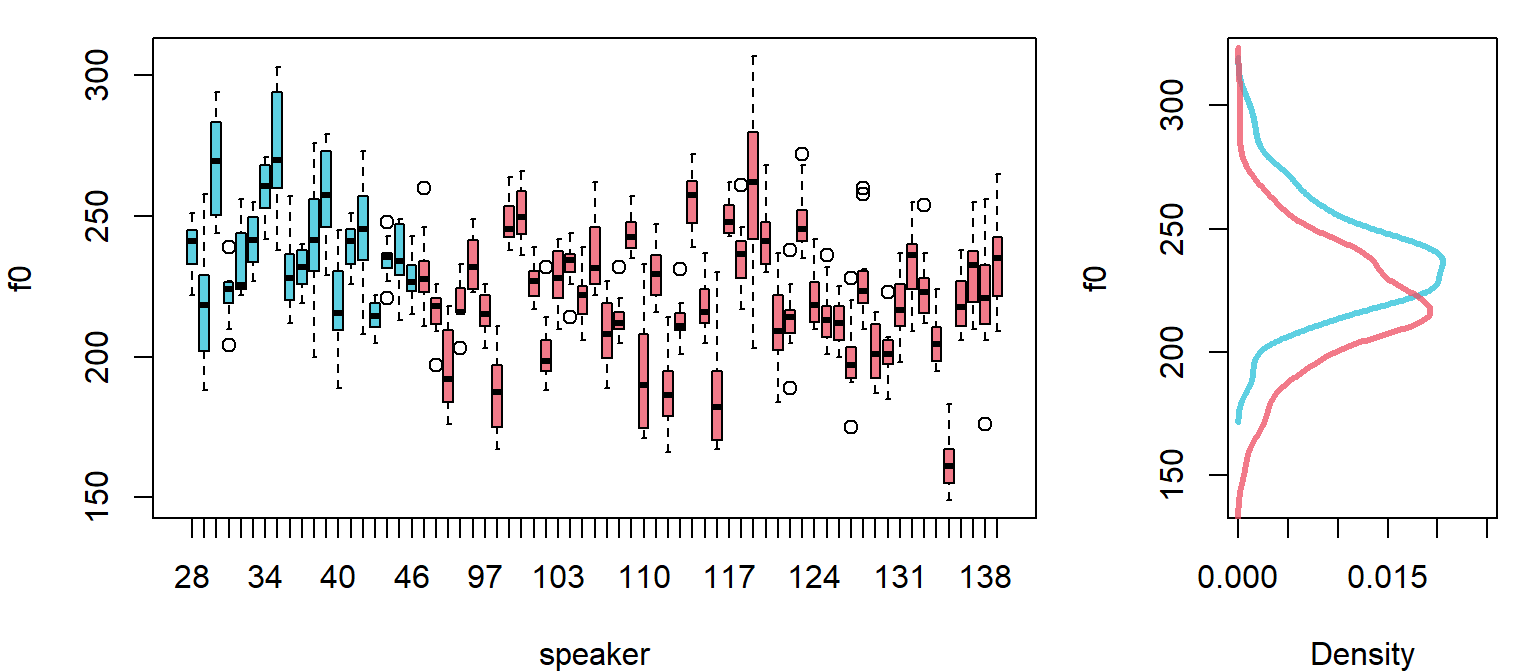
\includegraphics{03_files/figure-latex/F3-boxplots-density-1.pdf}
\caption{\label{fig:F3-boxplots-density}Comparison of f0 productions by individual girls (cyan) and women (red). Densities compare whole distributions.}
\end{figure}

\hypertarget{estimating-the-difference-between-two-means-with-brms}{%
\section{Estimating the difference between two means with `brms'}\label{estimating-the-difference-between-two-means-with-brms}}

In Chapter 2 the model we fit had the simplest possible formula, just an intercept. Here, we need to extend this to include an actual predictor: a vector indicating `adultness'. Remember that formulas look like this \texttt{y\ \textasciitilde{}\ predictor}. Previously, our formula had no predictors and so it looked like this \texttt{f0\ \textasciitilde{}\ 1\ +\ (1\textbar{}speaker)}, where the \texttt{1} indicates that this is an intercept-only model.

If we want to predict f0 based on whether the talker is an adult or not, our model is going to need a formula that looks like this \texttt{f0\ \textasciitilde{}\ adult\ +\ (1\textbar{}speaker)}. This assumes that we have a column in our dataframe that indicates whether each data point was produced by an adult or not, and that this column is called \texttt{adult}. This model formula basically says `we expect f0 to vary around the intercept based on whether the talker is an adult or not, in addition to speaker-specific adjustments to the intercept'. Recall that you only need to include a \texttt{1} in your model formula if you \emph{only} have an intercept. If you at least one predictor you don't need to specifically add the \texttt{1} in your formula, the intercept is added automatically.

The model specified by this formula \texttt{f0\ \textasciitilde{}\ adult\ +\ (1\textbar{}speaker)} calculates an intercept (mean value) for each speaker. However, note that it does \textbf{not} include an effect for \texttt{adult} for each speaker (i.e., the model does \emph{not} include a term like \texttt{(adult\textbar{}speaker)}). This means that although the model calculates an intercept for each speaker, it does not calculate an effect for \texttt{adult} fror each speaker. This is because we can estimate a mean for each speaker, but we cannot estimate the effect for `adultness' for each speaker. Each speaker is only either an adult or a child, and so we cannot estimate the effect for `adultness' for each speaker.

What would happen if you \emph{did} try to fit a model that doesnt `make sense' like \texttt{f0\ \textasciitilde{}\ adult\ +\ (adult\textbar{}speaker)}? Doing things that don't `make sense' from the model's perspective will cause it to crash or return strange values. Your model will not converge, your parameters will have strange values, or your credible intervals will be enourmous or perhaps too small. It's a good thing to keep in mind: if your model output just makes no sense to you at all and something strange seems to have gone wrong, the model may be specified in a way that is not supportable by the data.

Usually, I would discuss the specific structure of this model now, \emph{before} fitting the model. We're just going to put this off for a little bit because an explanation involves some of the less intuitive concepts relating to regression. We're going to to fit the model first and discuss its structure, and then get to the details of the model later in the chater, by which point they should make more sense.

\hypertarget{fitting-the-model-1}{%
\subsection{Fitting the model}\label{fitting-the-model-1}}

We load the \texttt{brms} package and fit the model, using the formula discussed above. Notice that I now include a prior for \texttt{class\ =\ "b"}, which is the class for all predictors that are not the intercept. Our model now includes a non-intercept term, and so I need to include this prior. Weakly informative priors of the same kind as discussed in Chapter 2 were used. For example, the prior set for \texttt{class\ =\ "b"} indicates that we expect the difference between groups in our model, in this case in the f0 of girls and women, to be between -200 and +200 Hz.

\begin{Shaded}
\begin{Highlighting}[]
\FunctionTok{library}\NormalTok{ (brms)}
\end{Highlighting}
\end{Shaded}

\begin{Shaded}
\begin{Highlighting}[]
\CommentTok{\# Fit the model yourself, or download pre{-}fit model from: }
\CommentTok{\# github.com/santiagobarreda/stats{-}class/tree/master/models}
\CommentTok{\# and load it using the next line, after placing in working directory}
\CommentTok{\# model = readRDS (\textquotesingle{}3\_model.RDS\textquotesingle{})}

\FunctionTok{set.seed}\NormalTok{ (}\DecValTok{1}\NormalTok{)}
\NormalTok{model }\OtherTok{=}  
\NormalTok{  brms}\SpecialCharTok{::}\FunctionTok{brm}\NormalTok{ (f0 }\SpecialCharTok{\textasciitilde{}}\NormalTok{ adult }\SpecialCharTok{+}\NormalTok{ (}\DecValTok{1}\SpecialCharTok{|}\NormalTok{speaker), }\AttributeTok{data =}\NormalTok{ females, }\AttributeTok{chains =} \DecValTok{4}\NormalTok{, }\AttributeTok{cores =} \DecValTok{4}\NormalTok{,}
       \AttributeTok{warmup =} \DecValTok{1000}\NormalTok{, }\AttributeTok{iter =} \DecValTok{11000}\NormalTok{, }\AttributeTok{thin =} \DecValTok{10}\NormalTok{,}
       \AttributeTok{prior =} \FunctionTok{c}\NormalTok{(}\FunctionTok{set\_prior}\NormalTok{(}\StringTok{"student\_t(3, 220, 100)"}\NormalTok{, }\AttributeTok{class =} \StringTok{"Intercept"}\NormalTok{),}
                 \FunctionTok{set\_prior}\NormalTok{(}\StringTok{"student\_t(3, 0, 100)"}\NormalTok{, }\AttributeTok{class =} \StringTok{"b"}\NormalTok{),}
                 \FunctionTok{set\_prior}\NormalTok{(}\StringTok{"student\_t(3, 0, 100)"}\NormalTok{, }\AttributeTok{class =} \StringTok{"sd"}\NormalTok{),}
                 \FunctionTok{set\_prior}\NormalTok{(}\StringTok{"student\_t(3, 0, 100)"}\NormalTok{, }\AttributeTok{class =} \StringTok{"sigma"}\NormalTok{)))}
\end{Highlighting}
\end{Shaded}

\hypertarget{interpreting-the-model}{%
\subsection{Interpreting the model}\label{interpreting-the-model}}

We can inspect the model print statement, which is mostly familiar by now.

\begin{Shaded}
\begin{Highlighting}[]
\CommentTok{\# inspect model}
\NormalTok{model}
\DocumentationTok{\#\#  Family: gaussian }
\DocumentationTok{\#\#   Links: mu = identity; sigma = identity }
\DocumentationTok{\#\# Formula: f0 \textasciitilde{} adult + (1 | speaker) }
\DocumentationTok{\#\#    Data: females (Number of observations: 804) }
\DocumentationTok{\#\# Samples: 4 chains, each with iter = 11000; warmup = 1000; thin = 10;}
\DocumentationTok{\#\#          total post{-}warmup samples = 4000}
\DocumentationTok{\#\# }
\DocumentationTok{\#\# Group{-}Level Effects: }
\DocumentationTok{\#\# \textasciitilde{}speaker (Number of levels: 67) }
\DocumentationTok{\#\#               Estimate Est.Error l{-}95\% CI u{-}95\% CI Rhat Bulk\_ESS Tail\_ESS}
\DocumentationTok{\#\# sd(Intercept)    19.13      1.79    15.97    22.94 1.00     2785     3504}
\DocumentationTok{\#\# }
\DocumentationTok{\#\# Population{-}Level Effects: }
\DocumentationTok{\#\#            Estimate Est.Error l{-}95\% CI u{-}95\% CI Rhat Bulk\_ESS Tail\_ESS}
\DocumentationTok{\#\# Intercept    220.47      2.88   214.73   226.00 1.00     1682     2515}
\DocumentationTok{\#\# adultchild    17.76      5.21     7.80    28.30 1.00     2104     3184}
\DocumentationTok{\#\# }
\DocumentationTok{\#\# Family Specific Parameters: }
\DocumentationTok{\#\#       Estimate Est.Error l{-}95\% CI u{-}95\% CI Rhat Bulk\_ESS Tail\_ESS}
\DocumentationTok{\#\# sigma    12.95      0.34    12.30    13.62 1.00     4005     3775}
\DocumentationTok{\#\# }
\DocumentationTok{\#\# Samples were drawn using sampling(NUTS). For each parameter, Bulk\_ESS}
\DocumentationTok{\#\# and Tail\_ESS are effective sample size measures, and Rhat is the potential}
\DocumentationTok{\#\# scale reduction factor on split chains (at convergence, Rhat = 1).}
\end{Highlighting}
\end{Shaded}

However, there is a new predictor in the section on \texttt{Population-Level\ Effects}:

\begin{Shaded}
\begin{Highlighting}[]
\DocumentationTok{\#\#            Estimate Est.Error l{-}95\% CI u{-}95\% CI Rhat Bulk\_ESS Tail\_ESS}
\DocumentationTok{\#\# Intercept    220.47      2.80   215.10   226.16 1.00     1827     2813}
\DocumentationTok{\#\# adultchild    17.63      5.22     7.34    27.88 1.00     1987     2068}
\end{Highlighting}
\end{Shaded}

In addition to the `Intercept' term, we now get estimates for a term called \texttt{adultchild}. Admittedly, this is a strange name, but its how R handles predictors that are words (called `factors' in R). In general, R names predictors like these \texttt{factornameFactorlevel}. For example, a factor called \texttt{colors} with levels \texttt{red}, \texttt{green} and \texttt{blue} would have the levels \texttt{colorsred}, \texttt{colorsgreen}, and \texttt{colorsblue}. So, the \texttt{adultchild} name tells us is that this is the estimate for the \texttt{child} level of the \texttt{adult} factor.

A couple of questions arise. First, the `Intercept' term in the model above seems to correspond to the mean f0 for adult females. We can confirm this:

\begin{Shaded}
\begin{Highlighting}[]
\CommentTok{\# calculate means of f0 based on values of adult vector}
\FunctionTok{aggregate}\NormalTok{ (f0 }\SpecialCharTok{\textasciitilde{}}\NormalTok{ adult, }\AttributeTok{data =}\NormalTok{ females, }\AttributeTok{FUN =}\NormalTok{ mean)}
\DocumentationTok{\#\#   adult       f0}
\DocumentationTok{\#\# 1 adult 220.4010}
\DocumentationTok{\#\# 2 child 238.3509}
\end{Highlighting}
\end{Shaded}

However, the estimate for children is 17.6 Hz, which is odd, and obviously can't be the actual mean f0 produced by these girls. Why can't it just be the actual value of the girls' f0? Although it might seem like this would be simpler, the fact is it wouldn't really work. To understand why, we're going to have to talk about contrasts

\hypertarget{contrasts}{%
\section{Contrasts}\label{contrasts}}

Contrasts are basically the numerical implementation of factors in your model. Factors are variables like `adult' vs.~`child' that are not inherently numerical. You may initially think that we can just separately estimate the women's average, the girl's average, and the overall mean. However, our models can't actually do this. The general problem is as follows. If you have two groups then you can't independently calculate all of:

\begin{enumerate}
\def\labelenumi{\arabic{enumi})}
\tightlist
\item
  group 1 mean.
\item
  group 2 mean.
\item
  the overall mean.
\end{enumerate}

Why not? Because once you know 2 of those things you know the 3rd. For example, if the group 1 mean is 5 and the overall mean is 6, obviously the group 2 mean \textbf{must} be 7. Why does this matter? Because when things are entirely predictable based on each other, they are not actually separate things, even though they may seem that way to us. When things are entirely predictable in this way we say they are linearly dependent, and regression models don't like this. Here's three perspectives on why this is a problem:

\begin{enumerate}
\def\labelenumi{\arabic{enumi})}
\item
  Imagine you were trying to predict a person's weight from their height. You want to include height in centimeters \emph{and} height in meters in your model, and you want to independently estimate effects for both predictors. Since height in centimeters = height in meters / 100, that is obviously not going to be possible. The effect of one must be 100 times the effect of the other! Even though it may be less transparent, this is the same reason why we can't estimate all the group means \emph{and} the overall mean.
\item
  With two groups, or any two points in a space, you can estimate one distance, not two. If each group could really be a different distance from the mean, you would need to estimate \emph{two} distances. How can you estimate two separate distances given only two points? With two points, we are really only in a position to estimate \emph{one} difference, that between our two group averages.
\item
  When we had one group we obviously couldn't get the overall mean independently from the sample mean. All we had was one sample mean, and that was our best estimate of the Intercept too. Adding 1 more group allows us to calculate 1 more mean (the new group mean), not two (the new group mean and the intercept). That would mean adding a second group (with 1 mean) somehow contributed twice as much information as the first group did. Instead, adding a second mean changes our best guess for the population mean: it is now between the two groups. However, this information is not independent from the value of the two group means.
\end{enumerate}

\hypertarget{treatment-coding}{%
\subsection{Treatment coding}\label{treatment-coding}}

The coding scheme you use determines how your model represents the differences it encodes. In the model above we used `treatment' coding (the default in R). In treatment coding, a `reference' level is chosen to be the intercept, and all group effects reflect the difference between the mean for that group, and the value of the Intercept (i.e., the mean for the reference level).

By default, R chooses the alphabetically-lowest level to be the reference level. That is why the Intercept in our model is equal to the mean of the `adult' group, the average for adult females. The effect for `child' (\texttt{adultchild}) represents the difference between the child mean and the adult mean. This means that our credible intervals also represent the \emph{difference} in the means and not the means themselves. So, we expect the \emph{difference} between girls and women in this sample to be about 17 Hz, and we think there is a 95\% chance that the \emph{difference} between the means is between 7.3 and 27.9 Hz in magnitude.

We can see how the effects estimates in our model resemble the means, or differences between means, in our sample.

\begin{Shaded}
\begin{Highlighting}[]
\CommentTok{\# calculate group means}
\FunctionTok{tapply}\NormalTok{ (females}\SpecialCharTok{$}\NormalTok{f0, females}\SpecialCharTok{$}\NormalTok{adult, mean)}
\DocumentationTok{\#\#    adult    child }
\DocumentationTok{\#\# 220.4010 238.3509}

\CommentTok{\# find the difference between them}
\FunctionTok{diff}\NormalTok{ (}\FunctionTok{tapply}\NormalTok{ (females}\SpecialCharTok{$}\NormalTok{f0, females}\SpecialCharTok{$}\NormalTok{adult, mean))}
\DocumentationTok{\#\#    child }
\DocumentationTok{\#\# 17.94984}
\end{Highlighting}
\end{Shaded}

To interpret treatment coded coefficients in a regression model:

\begin{itemize}
\item
  The reference category mean is the `Intercept' in the model.
\item
  The value of the coefficients of any other group effect are equal to \texttt{group\ mean\ -\ Intercept\ (reference\ group\ mean)}.
\item
  So, to recover the mean estimate for any other group, we add \texttt{group\ effect\ +\ Intercept\ (reference\ group\ mean)}.
\end{itemize}

\hypertarget{sum-coding}{%
\subsection{Sum coding}\label{sum-coding}}

There are multiple options for coding schemes, and the best one for you depends on what you want to get out of the model. Changing the coding scheme may substantially change the value of your coefficients and the way they should be interpreted. However, they will not change the fundamental relationships encoded in your model. As a result, the selection of a coding scheme best suited for a model depends on which one results in the simplest interpretation of the model given the purpose of the research.

That being said, going forward we will be focusing exclusively on what is known as `sum coding'. The reason for a focus on a single coding scheme is in order to save space and minimize confusion for the reader. The reason for selecting sum coding specifically is because it has some desirable mathematical properties and it allows models to be interpreted in a style reminiscent of a traditional ANOVA, which many researchers may find useful.

In sum coding, there is no reference level. Instead, the model Intercept represents the overall mean of all your groups. The effect for each individual group is then represented as a deviation from the Intercept, and all of these effects are constrained to sum to zero. Just like for treatment coding, you can't estimate all of your group means. When using sum coding, R selects the \emph{alphabetically last} level of your factor, and does not estimate it. However, the values of the missing effect is easy to recover algebraically since the sum of the coefficients must equal zero.

As a result of the sum-to-zero constraint, the missing factor level will always be equal to the \emph{negative sum} of the other factors. This means you add up the values of the levels that \emph{are} present, and flip the sign. The outcome is the value of your missing level. If you think about it, it must be this way. This is because the final missing value must cancel out the sum of the others if the sum of all the values is to equal zero.

As discussed earlier, with only two groups if you know the overall mean and the distance of one group to the mean, you also know the distance of the other group to the mean. This can be seen quite clearly below where the difference of each group to the overall mean is exactly -8.97. So, if our model tells us that the mean is 229.4 and the adult group is -8.97 Hz below this, then the child group \emph{must} be the negative sum of the other coefficients. In this case there is only one so we just flip the sign on it (i.e., - (-8.97)).

\begin{Shaded}
\begin{Highlighting}[]
\CommentTok{\# calculate group means}
\NormalTok{means }\OtherTok{=} \FunctionTok{tapply}\NormalTok{ (females}\SpecialCharTok{$}\NormalTok{f0, females}\SpecialCharTok{$}\NormalTok{adult, mean)}
\FunctionTok{mean}\NormalTok{ (means)}
\DocumentationTok{\#\# [1] 229.376}

\CommentTok{\# find the distances to the overall mean}
\NormalTok{means }\SpecialCharTok{{-}} \FunctionTok{mean}\NormalTok{ (means)}
\DocumentationTok{\#\#     adult     child }
\DocumentationTok{\#\# {-}8.974918  8.974918}
\end{Highlighting}
\end{Shaded}

To interpret sum coded coefficients in regression models:

\begin{itemize}
\item
  The overall mean of all your groups is the `Intercept' in the model.
\item
  The value of the coefficients of any other group mean will be equal to \texttt{group\ mean\ -\ Intercept\ (overall\ mean)}.
\item
  To recover the mean estimate for any other group, we add \texttt{group\ effect\ +\ Intercept\ (overall\ mean)}.
\end{itemize}

\hypertarget{comparison-of-sum-and-treatment-coding}{%
\subsection{Comparison of sum and treatment coding}\label{comparison-of-sum-and-treatment-coding}}

The image below presents a comparison of the way the two coding schemes treat our data. In each case they estimate 1 intercept and one effect, letting you recreate 1 other mean (i.e., they each omit one parameter). In treatment coding the omitted value is the overall mean, which in the 2-group case will always be \texttt{Intercept\ +\ Effect/2}. In the case of sum coding the omitted value is the effect for the second group, which will always be the same magnitude but have the opposite sign as the effect for the first group (i.e., \texttt{-Effect} in a two-group model).

\begin{figure}
\includegraphics[width=1\linewidth]{./images/coding} \caption{Artists rendition of contrast and treatment coding differences for our data}\label{fig:contrast-figure}
\end{figure}

\hypertarget{refitting-the-model-with-sum-coding}{%
\section{Refitting the model with sum coding}\label{refitting-the-model-with-sum-coding}}

We're going to re-fit the model using sum coding, and see how the coefficients change (or don't).

\hypertarget{fitting-the-model-2}{%
\subsection{Fitting the model}\label{fitting-the-model-2}}

To fit a model with sum coding, we change the global contrast options in R. These options will be in effect until we restart R or change the contrasts to something else. If you fit a model with this coding, be sure to set this option every time you start R and want to work with this model. If there is a mismatch between your contrast settings and what the model expects there may be a problem.

\begin{Shaded}
\begin{Highlighting}[]
\CommentTok{\# to change to sum coding}
\FunctionTok{options}\NormalTok{ (}\AttributeTok{contrasts =} \FunctionTok{c}\NormalTok{(}\StringTok{\textquotesingle{}contr.sum\textquotesingle{}}\NormalTok{,}\StringTok{\textquotesingle{}contr.sum\textquotesingle{}}\NormalTok{))}

\CommentTok{\# to change back to treatment coding}
\CommentTok{\# options (contrasts = c(\textquotesingle{}contr.treatment\textquotesingle{},\textquotesingle{}contr.treatment\textquotesingle{}))}
\end{Highlighting}
\end{Shaded}

We can fit the same model with sum coding using the exact same code since the options have changed. Please keep in mind you will need to set this every time you start R, as it will reset to treatment coding each time it restarts. If fit a model with sum coding, you may need to change the default contrast to sum coding (as above) any time you work with the model, or some things may not work.

\begin{Shaded}
\begin{Highlighting}[]
\CommentTok{\# Fit the model yourself, or download pre{-}fit model from: }
\CommentTok{\# github.com/santiagobarreda/stats{-}class/tree/master/models}
\CommentTok{\# and load it using the next line, after placing in working directory}
\CommentTok{\# model\_sum\_coding = readRDS (\textquotesingle{}3\_model\_sum\_coding.RDS\textquotesingle{})}

\FunctionTok{set.seed}\NormalTok{ (}\DecValTok{1}\NormalTok{)}
\NormalTok{model\_sum\_coding }\OtherTok{=}  
\NormalTok{  brms}\SpecialCharTok{::}\FunctionTok{brm}\NormalTok{ (f0 }\SpecialCharTok{\textasciitilde{}}\NormalTok{ adult }\SpecialCharTok{+}\NormalTok{ (}\DecValTok{1}\SpecialCharTok{|}\NormalTok{speaker), }\AttributeTok{data =}\NormalTok{ females, }\AttributeTok{chains =} \DecValTok{4}\NormalTok{, }\AttributeTok{cores =} \DecValTok{4}\NormalTok{,}
       \AttributeTok{warmup =} \DecValTok{1000}\NormalTok{, }\AttributeTok{iter =} \DecValTok{11000}\NormalTok{, }\AttributeTok{thin =} \DecValTok{10}\NormalTok{,}
       \AttributeTok{prior =} \FunctionTok{c}\NormalTok{(}\FunctionTok{set\_prior}\NormalTok{(}\StringTok{"student\_t(3, 220, 100)"}\NormalTok{, }\AttributeTok{class =} \StringTok{"Intercept"}\NormalTok{),}
                 \FunctionTok{set\_prior}\NormalTok{(}\StringTok{"student\_t(3, 0, 100)"}\NormalTok{, }\AttributeTok{class =} \StringTok{"b"}\NormalTok{),}
                 \FunctionTok{set\_prior}\NormalTok{(}\StringTok{"student\_t(3, 0, 100)"}\NormalTok{, }\AttributeTok{class =} \StringTok{"sd"}\NormalTok{),}
                 \FunctionTok{set\_prior}\NormalTok{(}\StringTok{"student\_t(3, 0, 100)"}\NormalTok{, }\AttributeTok{class =} \StringTok{"sigma"}\NormalTok{)))}
\end{Highlighting}
\end{Shaded}

We are going to use the \texttt{fixef} function in \texttt{brms} to inspect only the \texttt{Population-Level\ Effects} in our model. This is just to save space because the rest of the model should look the same, but feel free to check out the print statement for the whole model.

The \texttt{Population-Level\ Effects} are also sometimes called \emph{fixed} effects, in part because they are `fixed' across the population. Forexample, the effect for `child' doesnt apply only to little Susie or Little Johnny in particular, but to \emph{children} broadly speaking.

\begin{Shaded}
\begin{Highlighting}[]
\CommentTok{\# inspect model}
\FunctionTok{fixef}\NormalTok{ (model\_sum\_coding)}
\DocumentationTok{\#\#             Estimate Est.Error      Q2.5      Q97.5}
\DocumentationTok{\#\# Intercept 229.294956  2.655493 224.17507 234.392211}
\DocumentationTok{\#\# adult1     {-}8.907178  2.698205 {-}14.19731  {-}3.545559}
\end{Highlighting}
\end{Shaded}

An inspection of the fixed effects shows that, as expected, the Intercept now reflects the overall mean and the single parameter reflects the distance of the adult mean to the overall mean. Note that the parameter is now called \texttt{adult1}. This is just how \texttt{brm} handles factors under sum coding. Predictors representing factors will be named \texttt{factornameN}, where \texttt{factorname} is the predictor name and \texttt{N} is the level number. Levels are ordered alphabetically starting at one, and the alphabetically-last level will not be estimated.

You can predict how your factor levels will be ordered by doing something like this:

\begin{Shaded}
\begin{Highlighting}[]
\FunctionTok{sort}\NormalTok{ ( }\FunctionTok{unique}\NormalTok{ (females}\SpecialCharTok{$}\NormalTok{adult))}
\DocumentationTok{\#\# [1] "adult" "child"}
\end{Highlighting}
\end{Shaded}

So, \texttt{adult1} in our model corresponds to the ``adult'' level of our predictor, and \texttt{adult2} \emph{would} be ``child'', but it is not separately estimated by our model (since \texttt{adult2\ =\ -adult1}).

\hypertarget{description-of-the-model-2}{%
\subsection{Description of the model}\label{description-of-the-model-2}}

Regression models try to break up values into their components. This is why effects are expressed in terms of differences to some reference value. For example, imagine I say that a person's average f0 is usually 220 Hz and under some condition their average f0 is also 220 Hz. Didn't I just say that this condition has no \emph{effect} on their f0? To say that this condition has no effect on mean f0 is to say, at least in art, that it causes no difference in mean f0.

On the other hand something that \emph{does} cause a difference in mean f0 \emph{does} have an effect on mean f0. We can express the effect of something in terms of the difference it causes. For example, we can say that under so and so conditions a person will tend to raise their f0 by 20 Hz, relative to some reference value.

More generally, we can think of any variable as the sum of a bunch of independent \emph{effects}. This is just a way to \emph{think} about variables, to break up observed values into their component parts. It should not be confused with the \emph{reality} of these values and the processes that underlie them (whatever that is!).

So far we have covered the fact that after picking a value to use as a reference point (the model intercept), our models:

\begin{itemize}
\item
  represent group means as deviations from the intercept.
\item
  represent the speaker-specific deviations from the intercept (\(\alpha_{speaker}\)) as being centered at 0, with a standard deviation of \(\sigma_{speaker}\).
\item
  represent the random error (\(\varepsilon\)) as having a mean of 0 and a standard deviation of \(\sigma_{error}\).
\end{itemize}

In each case, these model coefficients reflect \emph{deviations} from some reference point. As a result, when the parameters associated with different effects equal 0, this means that no effect is present.

\begin{itemize}
\item
  when group coefficients are 0 the group lies exactly at the intercept. In sum coding this is the overall mean, meaning that the group is just like the population in general.
\item
  when a speaker-effect is 0 this speaker is exactly average with respect to their group. This means there is nothing about this speaker (along this dimension) that is unpredictable given knowledge of their group.
\item
  when an error is 0 this production is exactly as expected for a given speaker.This means the production contains no error since it was an \emph{exactly} average (perfect?) production for that speaker.
\end{itemize}

If we think of our predictors as representing deviations from some reference value, we can `break up' any observed value into its component parts. For example, suppose that:

\begin{itemize}
\tightlist
\item
  the the overall mean is 229 Hz.
\item
  the adult female mean is 220 Hz.
\item
  a particular speaker has a mean f0 of 240 Hz.
\end{itemize}

If we observe a token with an f0 of 256 Hz produced by this speaker, that suggests the following decomposition:

256 = 229 (Intercept) - 9 (adult female effect) + 20 (speaker effect) + 16 (error)

This reflects the following considerations:

\begin{itemize}
\tightlist
\item
  the average f0 across the groups is 229 Hz.
\item
  the average for adult females is 9 Hz below the overall mean (229 - 9 = 220).
\item
  this speaker's average f0 is 20 Hz above the average for adult females (229 - 9 + 20 = 240).
\item
  this particular production is 16 Hz higher than expected for this particular speaker (229 - 9 + 20 + 16= 256).
\end{itemize}

Another observation from this talker might be:

237 = 229 (Intercept) - 9 (adult female effect) + 20 (speaker effect) - 3 (error)

In this case, the error is -3 since the production is now 3 Hz \emph{below} the speaker average. However, no other part of the equation has change since this is the same speaker in the same group. Regressions models basically carry out these decompositions for us, and reflect information regarding the average of these in their model parameters.

The full model specification, including prior probabilities is below. I used the same ordering format for the t-distributions that \texttt{brm} uses (nu, mean, sd).

The top chunk is labeled `likelihood' because this chunk specifies the relationships between our parameters and our data. As a result, the relationships specified in this section determine the likelihood of the model parameters. For example, in the first line we say that our data is normally distributed around some mean parameter. In turn, this specifies the shape of the likelihood function for that parameter given the data (as discussed in chapter 1). What I mean by this is that the shape of the likelihood functions for different model coefficients will be based on the relationships laid out in the section of the model description labeled `likelihood'.

\begin{equation}
\begin{split}
\textrm{Likelihood:} \\
f0_{[i]} \sim \mathcal{N}(\mu_{[i]},\sigma_{error}) \\
\mu_{[i]} = Intercept + adult1_{[adult_{[i]}]} + \alpha_{[speaker_{[i]}]} \\\\
\textrm{Priors:} \\
\alpha_{speaker} \sim \mathcal{N}(0,\sigma_{speaker}) \\ \\ 
Intercept \sim t(3, 220, 100) \\ 
adult1 \sim t(3, 0, 100) \\ 
\sigma_{error} \sim t(3, 0, 100) \\
\sigma_{speaker} \sim t(3, 0, 100) \\ 
\end{split}
\end{equation}

Here is how I would read this model description aloud in plain English:

\begin{quote}
``f0 is expected to vary according to a normal distribution with some unknown mean and standard deviation. Means are expected to vary based on whether the speaker was an adult or a child, and some speaker-dependent variation. The random speaker-dependent variation in means were modeled as coming from a normal distribution with a mean of 0 and an unknown standard deviation. Remaining parameters were given weakly informative t-distributed priors centered at 0, with standard deviations of 100, and with nu parameters equal to 3.''
\end{quote}

\hypertarget{interpreting-the-model-1}{%
\subsection{Interpreting the model}\label{interpreting-the-model-1}}

The \texttt{brms} package has several functions that make getting information from our models simple. We already mentioned the \texttt{fixef} function gets you means and 95\% credible intervals for all your `population level' parameters.

\begin{Shaded}
\begin{Highlighting}[]
\NormalTok{brms}\SpecialCharTok{::}\FunctionTok{fixef}\NormalTok{ (model\_sum\_coding)}
\end{Highlighting}
\end{Shaded}

\begin{verbatim}
##             Estimate Est.Error      Q2.5      Q97.5
## Intercept 229.294956  2.655493 224.17507 234.392211
## adult1     -8.907178  2.698205 -14.19731  -3.545559
\end{verbatim}

Using frequentist models, you cannot actually recover the parameters you did not estimate in your model. If you wanted to get these values, you would have to change the way you set the model up and fit it again. In contrast, Bayesian models allow you to compare any two (or more) parameters, as long as you follow some basic rules. This means that you will be able to recover estimates for any coefficient that your model was not able to specifically estimate.

You can see the individual samples for our parameters by calling the \texttt{fixef} function and setting \texttt{summary} to \texttt{FALSE}. Below, we see the first 6 posterior samples for each parameter.

\begin{Shaded}
\begin{Highlighting}[]
\NormalTok{samples }\OtherTok{=}\NormalTok{ brms}\SpecialCharTok{::}\FunctionTok{fixef}\NormalTok{ (model\_sum\_coding, }\AttributeTok{summary =} \ConstantTok{FALSE}\NormalTok{)}

\FunctionTok{head}\NormalTok{ (samples)}
\DocumentationTok{\#\#           parameters}
\DocumentationTok{\#\# iterations Intercept     adult1}
\DocumentationTok{\#\#       [1,]  226.3701 {-}12.265006}
\DocumentationTok{\#\#       [2,]  232.3973 {-}10.542661}
\DocumentationTok{\#\#       [3,]  230.6364 {-}11.296614}
\DocumentationTok{\#\#       [4,]  230.0953  {-}9.653068}
\DocumentationTok{\#\#       [5,]  227.6235  {-}9.229130}
\DocumentationTok{\#\#       [6,]  224.7867  {-}5.895867}
\end{Highlighting}
\end{Shaded}

To recover the group means for women and girls, we need to combine the Intercept and the group parameters. To do this properly, we need to manipulate these samples as necessary, and only summarize \emph{after} this process is complete. Combining parameters is deceptively simple. If we want to know what the um of \texttt{Intercept} and \texttt{adult1} is, all we need to do is sum the two columns together. This means we add the elements of each row together, resulting in a single vector as long as the two original columns.

Below I plot the individual samples and histograms for the \texttt{Intercept} (the overall mean), the \texttt{adult1} (the effect for adults) parameter, and the negative of the \texttt{adult} parameter (the effect for girls). I also present the combination of \texttt{Intercept+adult1}, which yields an estimate of the adult female mean.

\begin{verbatim}
##           parameters
## iterations Intercept     adult1
##       [1,]  226.3701 -12.265006
##       [2,]  232.3973 -10.542661
##       [3,]  230.6364 -11.296614
##       [4,]  230.0953  -9.653068
##       [5,]  227.6235  -9.229130
##       [6,]  224.7867  -5.895867
##       [7,]  224.5292  -8.052164
##       [8,]  228.5024 -12.911775
##       [9,]  230.1220 -11.996447
##      [10,]  235.2036 -13.041191
\end{verbatim}

\begin{figure}
\centering
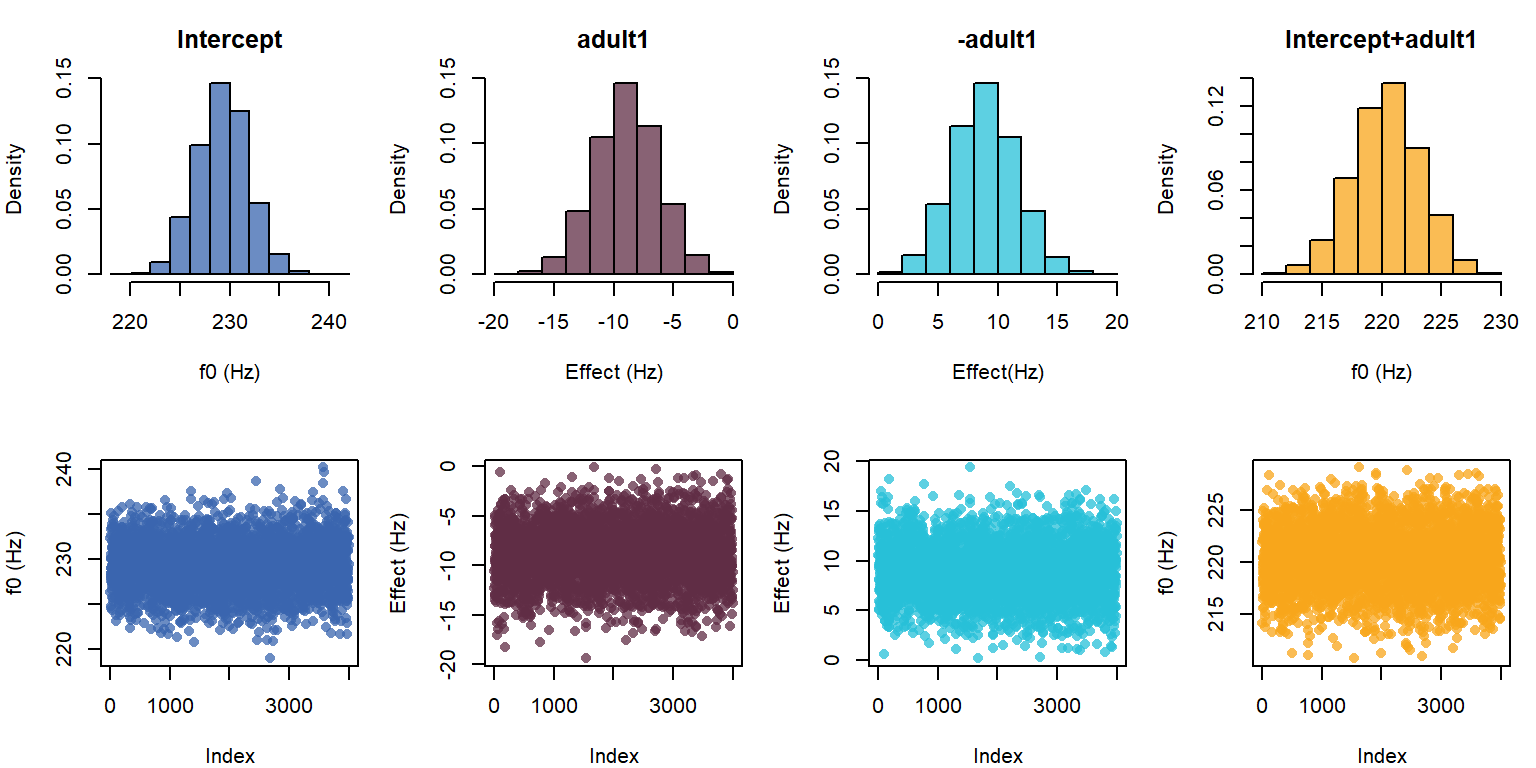
\includegraphics{03_files/figure-latex/F3-sample-boxplots-1.pdf}
\caption{\label{fig:F3-sample-boxplots}Comparison of histogram and trace plots of samples of selected parameters.}
\end{figure}

Remember that the summary statistics we make for our model parameters are nothing more than manipulations of these individual samples. In a very real sense, these samples \emph{are} our model. So, when we see the distribution of sample above, what we are looking at is the posterior distribution of more and less likely parameter values as determined by our data and model structure.

We can summarize the sum of the parameters using the \texttt{posterior\_summary} function, resulting in a mean, standard deviation, and credible interval for the new parameter:

\begin{Shaded}
\begin{Highlighting}[]
\CommentTok{\# calculate child mean}
\NormalTok{adult\_mean }\OtherTok{=}\NormalTok{ samples[,}\StringTok{\textquotesingle{}Intercept\textquotesingle{}}\NormalTok{] }\SpecialCharTok{+}\NormalTok{ samples[,}\StringTok{\textquotesingle{}adult1\textquotesingle{}}\NormalTok{]}

\CommentTok{\# report mean and spread of samples}
\NormalTok{brms}\SpecialCharTok{::}\FunctionTok{posterior\_summary}\NormalTok{ (adult\_mean)}
\DocumentationTok{\#\#      Estimate Est.Error     Q2.5    Q97.5}
\DocumentationTok{\#\# [1,] 220.3878  2.854104 214.6722 225.8792}
\end{Highlighting}
\end{Shaded}

Luckily, there is a function in \texttt{brms} called \texttt{hypothesis} that helps us add terms very easily, without having to do any of the above steps. You can ask the \texttt{hypothesis} function to add terms in your model (spelled just as they are in the print statement), and to compare the result to some number. If you compare the result to 0, it just tells you about the result of the terms you added.

For example, the line below says ``test my hypothesis that the Intercept plus the adult parameter is equal to zero''. This is a slightly convoluted way of saying "tell me what the value of the adult mean is so I can see if it is different from zero.

\begin{Shaded}
\begin{Highlighting}[]
\NormalTok{brms}\SpecialCharTok{::}\FunctionTok{hypothesis}\NormalTok{(model\_sum\_coding, }\StringTok{"Intercept + adult1 = 0"}\NormalTok{)[[}\DecValTok{1}\NormalTok{]][,}\DecValTok{1}\SpecialCharTok{:}\DecValTok{5}\NormalTok{]}
\DocumentationTok{\#\#               Hypothesis Estimate Est.Error CI.Lower CI.Upper}
\DocumentationTok{\#\# 1 (Intercept+adult1) = 0 220.3878  2.854104 214.6722 225.8792}
\end{Highlighting}
\end{Shaded}

The output above tells us our estimate for \texttt{Intercept\ +\ adult1}, which we know to be the expected mean f0 for adult females. Whereas the credible interval for the adult1 effect reflected uncertainty in the \emph{difference} between the adult1 mean and the Intercept, the credible interval provided above is now for the actual women's mean f0.

We can use the hypothesis function to confirm similar results for the model fit using treatment coding (\texttt{model}, fit above). In that model, the reference category was the adult female mean. So, if we call the \texttt{hypothesis} function on the intercept of the treatment-coding model, we can see that it will present similar values to those seen above.

\begin{Shaded}
\begin{Highlighting}[]
\NormalTok{brms}\SpecialCharTok{::}\FunctionTok{hypothesis}\NormalTok{(model, }\StringTok{"Intercept = 0"}\NormalTok{)[[}\DecValTok{1}\NormalTok{]][,}\DecValTok{1}\SpecialCharTok{:}\DecValTok{5}\NormalTok{]}
\DocumentationTok{\#\#        Hypothesis Estimate Est.Error CI.Lower CI.Upper}
\DocumentationTok{\#\# 1 (Intercept) = 0 220.4666  2.876742 214.7257 225.9976}
\end{Highlighting}
\end{Shaded}

We can check several parameter combinations simultaneously. Below I recreate all our mean estimates of interest, first for the sum coding model, and then for the treatment coding model. Notice that these models contain the same information, just represented in different ways.

\begin{Shaded}
\begin{Highlighting}[]
\NormalTok{brms}\SpecialCharTok{::}\FunctionTok{hypothesis}\NormalTok{(model\_sum\_coding, }
                 \FunctionTok{c}\NormalTok{(}\StringTok{"Intercept = 0"}\NormalTok{,   }\CommentTok{\# overall mean}
                   \StringTok{"Intercept + adult1 = 0"}\NormalTok{,  }\CommentTok{\# adult mean}
                   \StringTok{"Intercept {-} adult1 = 0"}\NormalTok{))[[}\DecValTok{1}\NormalTok{]][,}\DecValTok{1}\SpecialCharTok{:}\DecValTok{5}\NormalTok{] }\CommentTok{\# child mean}
\DocumentationTok{\#\#               Hypothesis Estimate Est.Error CI.Lower CI.Upper}
\DocumentationTok{\#\# 1        (Intercept) = 0 229.2950  2.655493 224.1751 234.3922}
\DocumentationTok{\#\# 2 (Intercept+adult1) = 0 220.3878  2.854104 214.6722 225.8792}
\DocumentationTok{\#\# 3 (Intercept{-}adult1) = 0 238.2021  4.529679 229.2861 247.1643}

\NormalTok{brms}\SpecialCharTok{::}\FunctionTok{hypothesis}\NormalTok{(model, }
                 \FunctionTok{c}\NormalTok{(}\StringTok{"Intercept + adultchild/2 = 0"}\NormalTok{,   }\CommentTok{\# overall mean}
                   \StringTok{"Intercept = 0"}\NormalTok{,  }\CommentTok{\# adult mean}
                   \StringTok{"Intercept + adultchild = 0"}\NormalTok{))[[}\DecValTok{1}\NormalTok{]][,}\DecValTok{1}\SpecialCharTok{:}\DecValTok{5}\NormalTok{] }\CommentTok{\# child mean}
\DocumentationTok{\#\#                     Hypothesis Estimate Est.Error CI.Lower CI.Upper}
\DocumentationTok{\#\# 1 (Intercept+adultchild/2) = 0 229.3454  2.696045 224.0355 234.5056}
\DocumentationTok{\#\# 2              (Intercept) = 0 220.4666  2.876742 214.7257 225.9976}
\DocumentationTok{\#\# 3   (Intercept+adultchild) = 0 238.2241  4.451373 229.6999 246.9899}
\end{Highlighting}
\end{Shaded}

If I were writing this is in a paper, at this point I could present this information in a paragraph. Based on the sum coded model, I would say something like:

``The overall mean f0 across all speakers was 229 Hz (sd = 2.7, 95\% CI = 224, 234). Adult female mean f0 was 220 Hz (sd = 2.9, 95\% CI = {[}215, 226{]}), while the mean f0 for girls was 228 Hz (sd = 4.28, 95\% CI = {[}230, 246{]}). The difference between the group means was 18 Hz on average (sd = 5.3, 95\% CI = {[}7, 28{]}), suggesting a small and noisy difference between groups, on average.''

Notice that to report the difference between groups, I have just doubled the value of the estimated effect for \texttt{adult1}. This is because this reflects the distance of each group to the intercept, and therefore \emph{half} of the distance between the two groups.

\hypertarget{random-effects}{%
\section{`Random' Effects}\label{random-effects}}

Below I present the speaker boxplot, with different colors for each group. So far we've discussed the speaker effects (\(\alpha_{speaker}\)), but we haven't actually done anything with them. One of the nice things about multilevel models is that we can actually estimate these parameters, and use them to answer our research questions.

Multilevel models are sometimes also called `random effects' or `mixed effects' models. What is `mixed' about them? Researchers often talk about whether effects are `fixed' or `random'. The general idea is that `fixed' effects are specifically chosen from a small set of possibilities, and we are not necessarily interested in the `other' levels.

For example, in this experiment we include children 10-12 and adults. Speaker age-groups don't really come from an infinite set of independent age-groups, not ones that will meaningfully affect our research questions anyways. Instead, categories like `adult' and `child' are chosen from a finite set of meaningful categories, and we are \emph{specifically} interested in the categories we've chosen. In this case, I really \emph{do} care about mean f0 for adults and not some other category I didn't sample.

In contrast, `random' effects are not chosen arbitrarily but at random. The speakers in our sample \emph{do} form part of a practically infinite sample. I am actually \emph{not} interested in the speakers I have but in what their behavior says about the speakers I did \emph{not} observe. In fact, most researchers would gladly trade perfect knowledge about any one speaker for even a small amount knowledge about a large set of speakers from the population.

Despite, or perhaps because of, this primarily philosophical distinction, in practice the terms `fixed' and `random' effects have \href{https://statmodeling.stat.columbia.edu/2005/01/25/why_i_dont_use/}{several inconsistent and sometimes contradictory definitions}.
Luckily, when thinking about these concepts in terms of multilevel models we can be very specific: `random' effects are parameters that we estimate as coming from distributions with unknown standard deviation terms. We treat speaker average f0 (\(\alpha_{speaker}\)) as coming from a normal distribution with a standard deviation parameter (\(\sigma_{speaker}\)) that is unknown and therefore estimated form the data. This is what makes this effect `random' in the context of a Bayesian multilevel model.

In contrast, notice that the effect for adultness was given a prior of \texttt{student\_t(3,\ 0,\ 100)}. We simply said the prior for this effect was 100, and we did this arbitrarily in a way that did not related to our data or model structure. For this reason, this effect (and effects estimated in this way) can be thought of as `random' effects.

\hypertarget{random-effects-priors-and-pooling}{%
\subsection{Random effects, priors and pooling}\label{random-effects-priors-and-pooling}}

If you look at our latest \texttt{brm} model fit, you'll notice that the standard deviation of the prior (\(\sigma_{speakers}\)) for the speaker-specific intercept deviations (\(\alpha_{speaker}\)) is not specifically defined in the model.

\begin{equation}
\begin{split}
\textrm{Priors:} \\
\alpha_{speaker} \sim \mathcal{N}(0,\sigma_{speaker}) \\ \\ 
Intercept \sim t(3, 220, 100) \\ 
adult1 \sim t(3, 0, 100) \\ 
\sigma_{error} \sim t(3, 0, 100) \\
\sigma_{speaker} \sim t(3, 0, 100) \\ 
\end{split}
\end{equation}

As noted above, the \(\sigma_{speaker}\) parameter is actually estimated from the data and not specified a priori. For this reason, the prior you set on \(\sigma_{speaker}\) is sometimes called a \emph{hyperprior}, because it's the prior for your prior!

By definition, the speaker effects are centered around 0 (the average). The only question is, how widely are they distributed? Well, what better way to answer this question than using the distribution present in the data itself? This means that the amount of variation you expect between speakers is based on the amount of between-speaker variation you observe. The idea is basically: is it believable that this one person be this far away from the `average'? Well, it depends on what everyone else looks like!

By estimating the prior for some parameters from the data itself, multilevel models can help \href{http://www.stat.columbia.edu/~gelman/research/published/multiple2f.pdf}{protect against problems that naturally arise when researchers compare many things}. This is because in a Bayesian analysis, the prior influences the estimates of your individual parameters. As a result, the variation in the \emph{other} parameters in your sample can influence any given parameter.

This process is sometimes referred to as `partial pooling', since it refers to the partial pooling of information across subjects. Using partial pooling means the subject estimates are neither completely independent nor totally merged. They actually end up influencing each other in a logical manner. Broadly speaking, individual observations that deviate from `typical' values of the population are maintained when there is good enough evidence for them. When there is weak evidence for them relative to the other observations in the sample, estimates may be brought closer to the group averages. As a result, partial pooling results in what is sometimes called `shrinkage', because extreme values get `shrunk' towards the overall mean.

In the context of a multilevel model `random effects' are those you estimate with partial pooling, meaning the prior is estimated from the data (e.g., \(\sigma_{speaker}\)), and can affect individual parameter estimates. In contrast, `fixed effects' are those predictors for which you set arbitrary priors before fitting the model. This means that `fixed' effects are all estimated independently and will not affect each other (at least through their priors).

Although the terms terms `fixed' and `random' effects are useful (and I continue to use them to describe my models), it is important to keep in mind that the philosophical distinction between `fixed' and `random' predictors outlined above is not relevant for the models we are discussing here. The real distinction is: do I want to fit every level totally independently as if they were all unrelated? Or do I want to use partial pooling in my estimates, thereby using all of the information present in my sample to protect against spurious findings?

In general, when you have many levels of a factor, it may be a good idea to include these as `random' effects, regardless of how `random' it might actually be. There is not much downside to it: you get more information from the model (e.g., information about \(\sigma_{predictor}\)), and you can always fit multiple models to see what, if any differences, result form the different approaches.

Some useful things to consider are also: Do you believe that treating a predictor as a `random' effect offers a modeling advantage? Does it better reflect the process/relationships you are trying to understand? Does it provide you with information you find useful? Is it realistic to fit this kind of model given the amount of data you have, and the nature of the relationships in the data? Right now the last point is not something we have talked about very much, but it is something we will need to worry about more as our models become more complicated.

\hypertarget{inspecting-the-random-effects}{%
\subsection{Inspecting the random effects}\label{inspecting-the-random-effects}}

The \texttt{brms} package has several functions to help understand our `random' effects. First, there is a function called \texttt{ranef} which returns random effects estimates in the same way that \texttt{fixef} provides fixed effects estimates. The leftmost column of the output below represents the estimated effects associated with each speaker average value.

\begin{Shaded}
\begin{Highlighting}[]
\CommentTok{\# I am telling it to give me the \textquotesingle{}speaker\textquotesingle{} Intercepts, but only the first }
\CommentTok{\# 10 rows. This is just so it doesn\textquotesingle{}t take up the whole page.}
\NormalTok{speaker\_effects }\OtherTok{=}\NormalTok{ brms}\SpecialCharTok{::}\FunctionTok{ranef}\NormalTok{ (model\_sum\_coding)}\SpecialCharTok{$}\NormalTok{speaker[,,}\StringTok{"Intercept"}\NormalTok{]}
\NormalTok{speaker\_effects[}\DecValTok{1}\SpecialCharTok{:}\DecValTok{10}\NormalTok{,]}
\DocumentationTok{\#\#      Estimate Est.Error       Q2.5     Q97.5}
\DocumentationTok{\#\# 28   1.184333  5.735588 {-}10.186326 12.319648}
\DocumentationTok{\#\# 29 {-}19.671885  5.652084 {-}30.928433 {-}8.422325}
\DocumentationTok{\#\# 30  28.536109  5.699914  17.484917 39.532266}
\DocumentationTok{\#\# 31 {-}14.595541  5.644469 {-}25.588406 {-}3.446464}
\DocumentationTok{\#\# 32  {-}4.510115  5.729995 {-}15.798335  6.980625}
\DocumentationTok{\#\# 33   2.628343  5.700041  {-}8.534003 13.893796}
\DocumentationTok{\#\# 34  20.503843  5.717652   9.210887 31.870600}
\DocumentationTok{\#\# 35  34.126366  5.738375  23.049256 45.605675}
\DocumentationTok{\#\# 36  {-}8.766414  5.776124 {-}20.133993  2.958266}
\DocumentationTok{\#\# 37  {-}6.289746  5.633946 {-}17.088190  4.926895}
\end{Highlighting}
\end{Shaded}

Notice that the speaker averages vary around 0, and some are even negative. That is because the speaker effects (and all random effects) are coded using sum-coding. Before when we only had an intercept the speaker averages encoded deviation from the overall mean. However, since our model encodes both the overall average \emph{and} the group means, the speaker-effects now represent differences to the group means and not to the overall means. So, the speaker-specific mean terms tell us: what is the average value for this speaker, relative to their group mean?

For example, we see that the mean for the second speaker above is -19.7 Hz. This means that they have a lower f0 than `expected', and their mean f0 is 19.7 Hz lower than their group mean f0. In contrast, the first speaker has a speaker mean effect that is nearly zero (1.2). That tells you that this speaker's mean f0 was nearly the same as that of the average for their group.

We can use a simple plotting function I wrote (\texttt{brmplot}) to look at the distribution of speaker effects terms. The function takes in the summaries made by \texttt{brms} and plots a point for each parameter mean/median, and lines indicating the credible intervals calculated by \texttt{brm} (usually 95\% credible intervals).

\begin{Shaded}
\begin{Highlighting}[]
\FunctionTok{par}\NormalTok{ (}\AttributeTok{mfrow =} \FunctionTok{c}\NormalTok{(}\DecValTok{1}\NormalTok{,}\DecValTok{1}\NormalTok{), }\AttributeTok{mar =} \FunctionTok{c}\NormalTok{(}\DecValTok{4}\NormalTok{,}\DecValTok{4}\NormalTok{,}\DecValTok{1}\NormalTok{,}\DecValTok{1}\NormalTok{))}
\FunctionTok{brmplot}\NormalTok{(speaker\_effects, }\AttributeTok{col =}\NormalTok{ colors)}
\FunctionTok{abline}\NormalTok{ (}\AttributeTok{h=}\DecValTok{0}\NormalTok{)}
\end{Highlighting}
\end{Shaded}

\begin{figure}
\centering
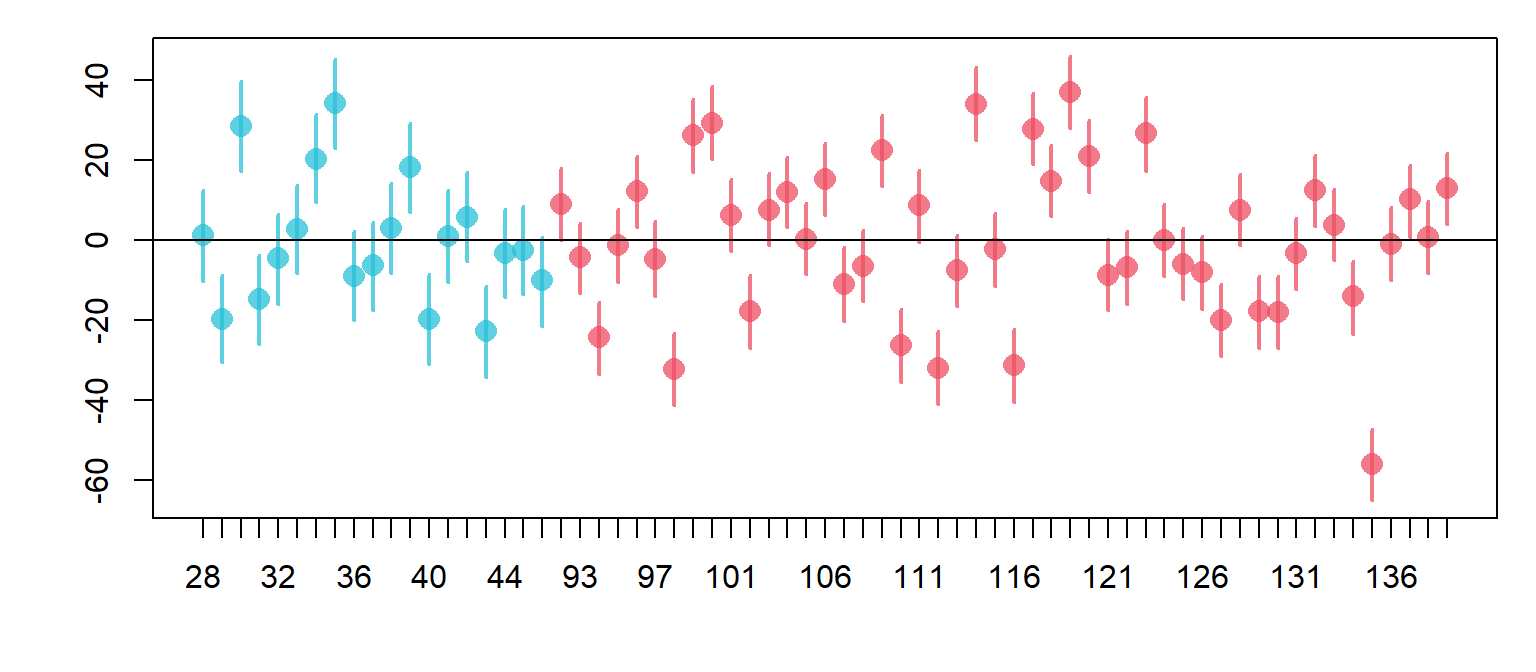
\includegraphics{03_files/figure-latex/brm-random-effects-1.pdf}
\caption{\label{fig:brm-random-effects}Posterior estimates of speaker 'random intercepts for girls (cyan) and women (red). Points indicate means, bars indicate 95\% credible intervals.}
\end{figure}

We can compare the estimates of by-speaker intercepts to the distribution of actual data arranged by subject, indicating a close correspondence. We can also note that all of the speaker random effects are centered at zero so that these do not reflect the 18 Hz group difference seen between the adult females and girls in our data.

\begin{Shaded}
\begin{Highlighting}[]
\DocumentationTok{\#\# plot comparison of estimates of speaker means to actual data}
\FunctionTok{par}\NormalTok{ (}\AttributeTok{mfrow =} \FunctionTok{c}\NormalTok{(}\DecValTok{1}\NormalTok{,}\DecValTok{2}\NormalTok{), }\AttributeTok{mar =} \FunctionTok{c}\NormalTok{(}\DecValTok{4}\NormalTok{,}\DecValTok{4}\NormalTok{,}\DecValTok{1}\NormalTok{,}\DecValTok{1}\NormalTok{))}
\FunctionTok{brmplot}\NormalTok{( speaker\_effects, }\AttributeTok{col =}\NormalTok{ colors)}
\FunctionTok{boxplot}\NormalTok{ (f0 }\SpecialCharTok{\textasciitilde{}}\NormalTok{ speaker, }\AttributeTok{data=}\NormalTok{females, }\AttributeTok{col =}\NormalTok{ colors, }\AttributeTok{ylim =} \FunctionTok{c}\NormalTok{(}\DecValTok{150}\NormalTok{,}\DecValTok{310}\NormalTok{))}
\end{Highlighting}
\end{Shaded}

\begin{figure}
\centering
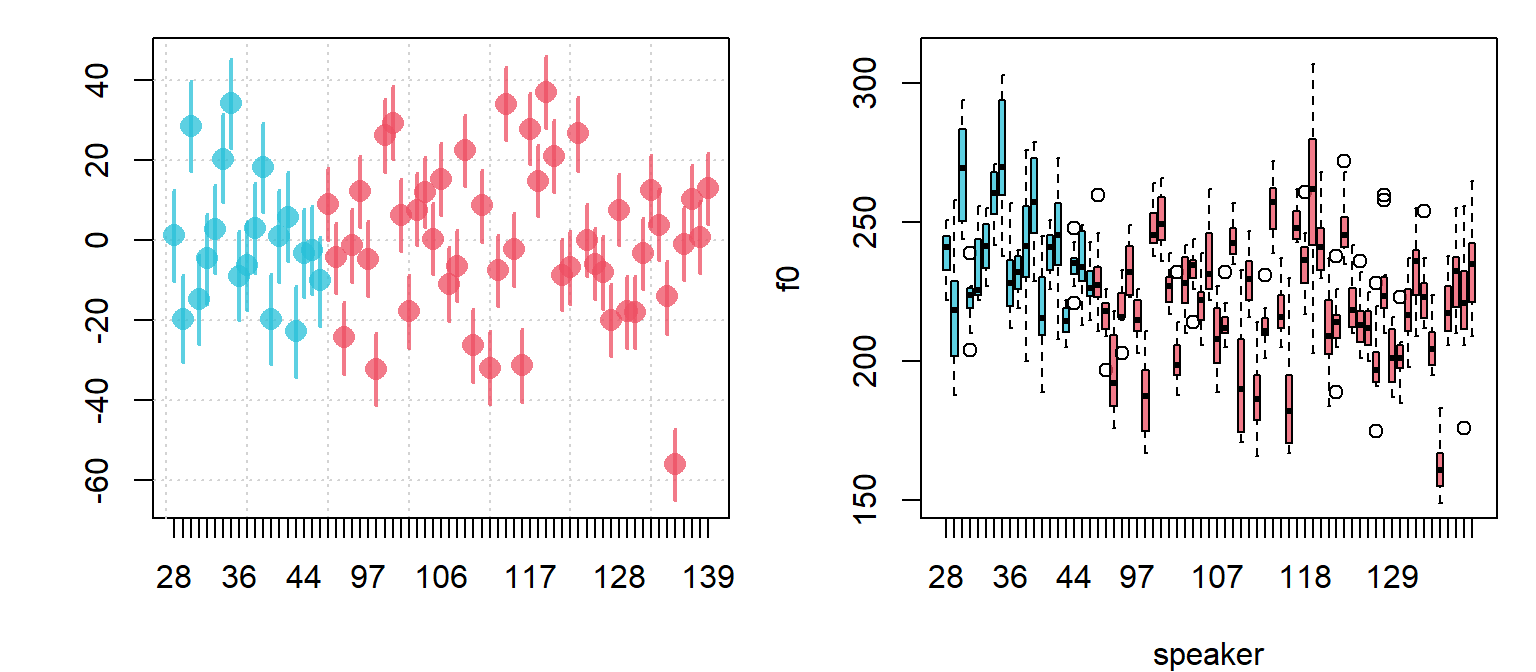
\includegraphics{03_files/figure-latex/brm-boxplot-comparison-1.pdf}
\caption{\label{fig:brm-boxplot-comparison}Comarisons of random speaker effects to the distribution of productions for the same speakers, for girls (cyan) and women (red).}
\end{figure}

\hypertarget{but-what-does-it-all-mean}{%
\section{But what does it all mean?}\label{but-what-does-it-all-mean}}

We have fit and interpreted the model, discussed the details of the results and seen several representations of the data. At this point we need to think about what it all `means'. At this point we need to think about how we might answer our question, ``so are the f0s produced by women and girls different?'' based on everything we have seen so far. First, consider the distribution of productions between and within speakers and groups, as shown in the figure below.

\begin{figure}
\centering
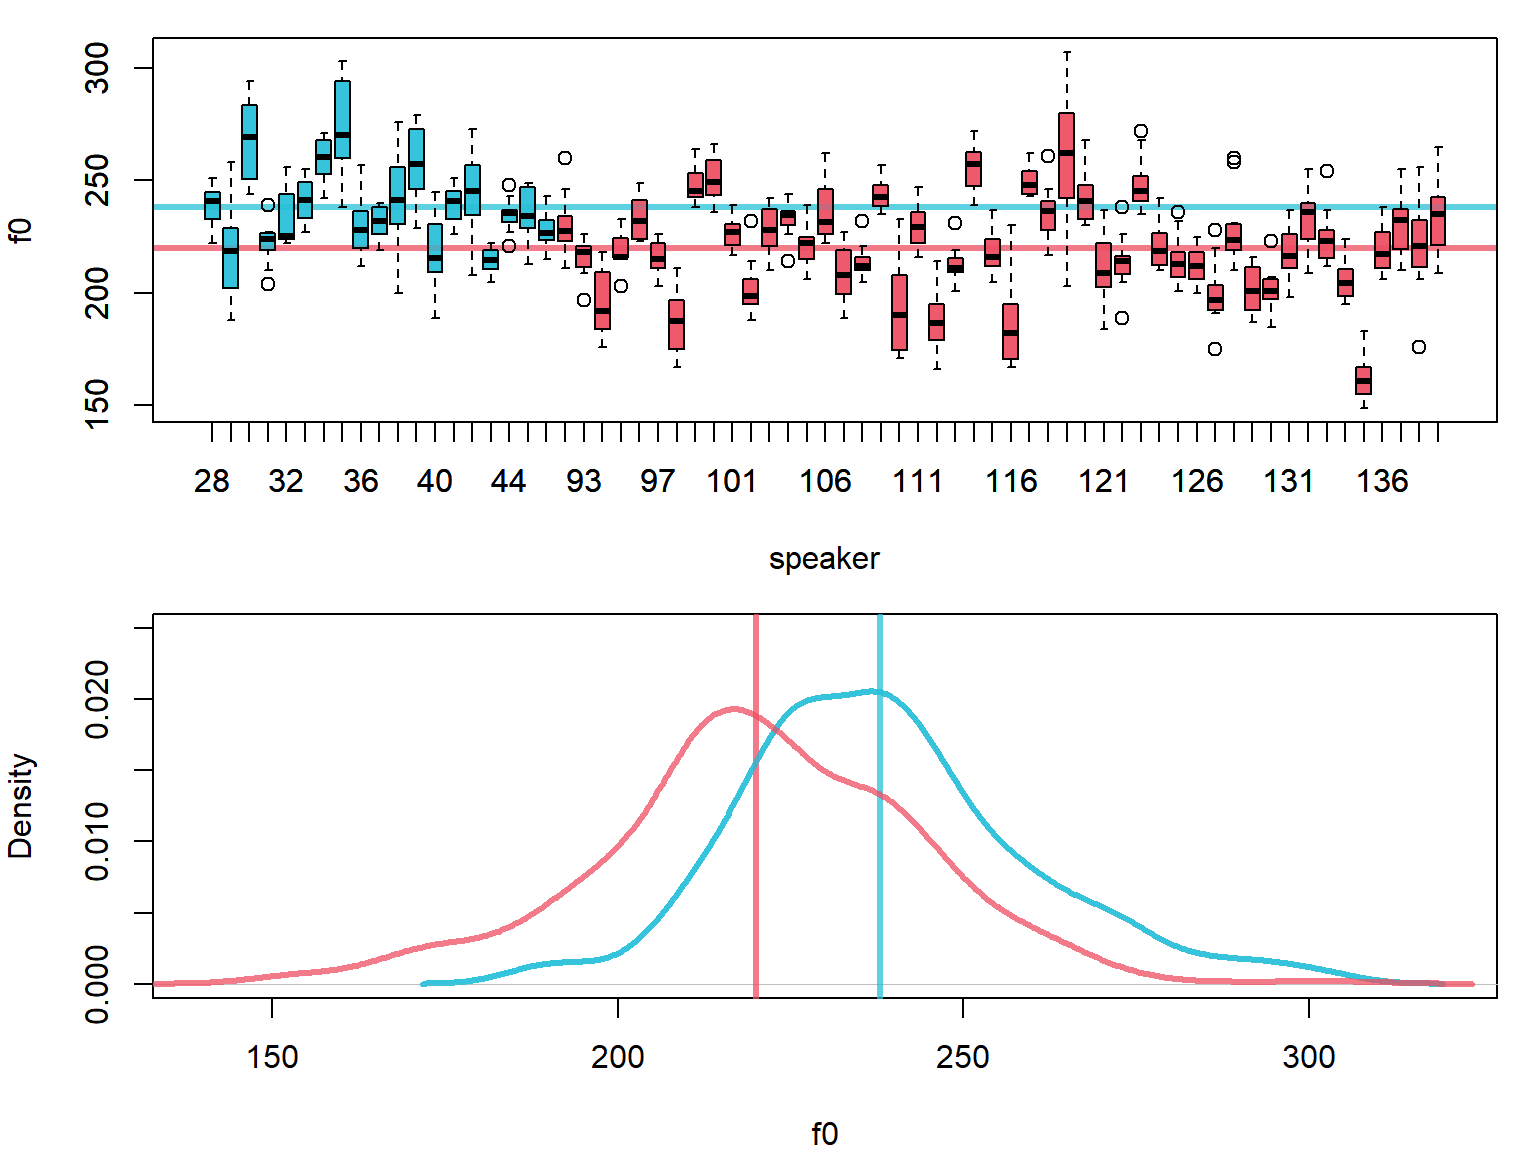
\includegraphics{03_files/figure-latex/F3-final-analysis-1.pdf}
\caption{\label{fig:F3-final-analysis}(left) Speaker boxplots for f0. Horizontal lines indicate the averages for girls (cyan) and women (red). (right) Densities of overall distributions for girls, and women.}
\end{figure}

An impartial look at our results (and figures) so far suggests that:

\begin{itemize}
\item
  the magnitude of between speaker variation is \textbf{larger} than the difference between girls and women (19 Hz vs 18/17 Hz). This means that random people drawn from the two groups largely overlap.
\item
  the magnitude of within-speaker variation (12 Hz) is almost as large as the group difference and the between-speaker difference (18 Hz)! This means that two random productions from two different people might be the same, even when the speakers average f0s are quite different.
\end{itemize}

And yet:

\begin{itemize}
\item
  the mean f0 \textbf{is} reliably different between women and girls, and there are well-known anatomical reasons for this that are expected a priori (i.e., adult females are larger than younger women, larger speakers often produce lower f0s). So, it's not like this result would be terribly surprising or unbelievable.
\item
  the between-speaker differences are `random' from person to person, but systematic for a given person. So, it's not clear why this would mean we should disregard group differences
\item
  even the within-speaker variation may be systematic given a more-complicated model. Perhaps what seems to be random variation is dependent on vowel quality or some other predictor we have not yet considered.
\end{itemize}

Ok, so are they different yes or no? Statistics aside, a fair assessment of our data suggests that neither binary conclusion is fully supported: they are distinguishable but overlap substantially. If you want to use this model to highlight the differences between girls and women, I think that is valid. I also think it would be valid to use this data to talk about between and within-speaker variation, highlighting the overlap that exists between speakers. Both are true! To a large extent, the meaning is as much in our heads as it is in the model, and we are free to interpret the results as we see fit, as long as reviewers (and readers in general) will believe us. The model is simply a reflection of the relationships in our data, and the interpretation is up to us.

Keep in mind that the ``as long as reviewers (and readers in general) will believe us'' component is crucial. The results of the model will need to be interpreted in the larger context of the work it is presented in, and in terms of scientific and general knowledge that readers have. The results of any model will need to `make sense' given this, and a statistical result on its own will not be enough to make people (including us) believe outlandish, or even weakly supported claims.

The model is not reality and should not be confused with reality. This is a very important point! A statistical finding does not \emph{prove} that something is \emph{true}. This kind of thinking has \href{https://slate.com/health-and-science/2017/06/daryl-bem-proved-esp-is-real-showed-science-is-broken.html}{caused many problems for researchers in the social sciences recently}. In general, we can imagine that 10 people might approach any given research question in 10 different ways, a concept known as \href{https://en.wikipedia.org/wiki/Researcher_degrees_of_freedom}{researcher degrees of freedom}. This would cause slight differences in their results, resulting in a sort of `distribution' for any given result. How can a fixed underlying reality result in a distribution or results? When they are all slightly wrong!

For example, we know for a fact that f0 varies, weakly but systematically, across vowel categories, a concept known as \href{https://www.sciencedirect.com/science/article/abs/pii/S0095447095801650}{intrinsic f0}. A model that included vowel category as a within-speaker predictor would reduce the apparent error in our model (making \(\sigma_{error}\) smaller), and might affect the precision of our other estimates. Would this new model invalidate our current model? Answering yes to this question is generally problematic because there is \emph{always} a better model out there, and so every model would automatically be invalid.

The solution is to think of your model not as a mathematical implementation of \emph{reality} but instead as a mathematical implementation of your research questions. Your model should include the information and structure that you think are necessary to represent and investigate your questions. Using a different model can result in different results given the same data, but asking a different question can also lead to different results given then same data! One of my favorite phrases to use is ``given our data and model structure''. This phrase is helpful because it highlights the fact that your results are contingent on:

\begin{enumerate}
\def\labelenumi{\arabic{enumi})}
\item
  the data you collected. Given other data you may have come to other conclusions.
\item
  the model you chose. Given another model you may have come to other conclusions.
\end{enumerate}

\hypertarget{simulating-the-two-group-model}{%
\section{Simulating the two-group model}\label{simulating-the-two-group-model}}

As in the last chapter, we're going to make fake data that's just like our real data, and break it up into its component parts. I'm going to focus on the sum coding model, and will mostly focus on what's different compared to the model simulated in the last chapter. For more detail about the simulation please see the simulation section in chapter 2.

First, there is an intercept equal to 229.3 Hz. The next step is to create a vector of length two that contains the effects for the adult and child groups. Notice that I am \textbf{not} drawing these values from a probability distribution. I am treating these as effects as fixed, meaning I am acting like they will contribute the same value to any given simulation. In contrast, note that the \texttt{alpha\_speaker} parameters (representing \(\alpha_{speaker}\)) \emph{are} drawn from a probability distribution. This is because every time we simulate we may encounter different subjects with different subject-specific effects.

In the line following the creation of \texttt{adult\_effect}, we create a vector indicating which adultness effect should be applied to each observation. We have 19 girls and 48 women in our sample, so we set the data up to have the same distribution (and include 12 tokens per speaker).

I want to highlight something that's very important about the way we are simulating our speaker effects. Just like our draw of \(\varepsilon\) do not distinguish between speakers, our draws of \(\alpha_{speaker}\) do not distinguish between groups. Notice that all 67 speaker effects are drawn from the same distribution of speakers below. This means that we think all speakers come from basically the same distribution, and that the mean of this distribution varies according to things like `adultness'. This may not be true, but this is what our model \emph{thinks} is true. \href{https://github.com/paul-buerkner/brms/issues/365}{\texttt{brms} makes it easy to change, and even test, these assumptions}, but we're not going to talk about that right now.

\begin{Shaded}
\begin{Highlighting}[]
\DocumentationTok{\#\# don\textquotesingle{}t run this line if you want a new simulated dataset. }
\FunctionTok{set.seed}\NormalTok{(}\DecValTok{1}\NormalTok{)}
\DocumentationTok{\#\# this is the value of our intercept}
\NormalTok{Intercept }\OtherTok{=} \FloatTok{229.3}
\DocumentationTok{\#\# this is a vector of adultness fixed effects}
\NormalTok{adult\_effect }\OtherTok{=} \FunctionTok{c}\NormalTok{(}\SpecialCharTok{{-}}\FloatTok{8.9}\NormalTok{, }\FloatTok{8.9}\NormalTok{)}
\DocumentationTok{\#\# this is a vector indicating which speaker produced which utterance}
\NormalTok{adult }\OtherTok{=} \FunctionTok{c}\NormalTok{(}\FunctionTok{rep}\NormalTok{ (}\DecValTok{2}\NormalTok{, }\DecValTok{19}\SpecialCharTok{*}\DecValTok{12}\NormalTok{), }\FunctionTok{rep}\NormalTok{ (}\DecValTok{1}\NormalTok{, }\DecValTok{48}\SpecialCharTok{*}\DecValTok{12}\NormalTok{))}
\DocumentationTok{\#\# this is a vector of 48 speaker effects}
\NormalTok{alpha\_speaker }\OtherTok{=} \FunctionTok{rnorm}\NormalTok{ (}\DecValTok{67}\NormalTok{, }\DecValTok{0}\NormalTok{, }\FloatTok{19.32}\NormalTok{)}
\DocumentationTok{\#\# this is a vector indicating which speaker produced which utterance}
\NormalTok{speaker }\OtherTok{=} \FunctionTok{rep}\NormalTok{ (}\DecValTok{1}\SpecialCharTok{:}\DecValTok{67}\NormalTok{, }\AttributeTok{each =} \DecValTok{12}\NormalTok{)}
\DocumentationTok{\#\# this vector contains the error}
\NormalTok{epsilon }\OtherTok{=} \FunctionTok{rnorm}\NormalTok{ (}\DecValTok{67}\SpecialCharTok{*}\DecValTok{12}\NormalTok{, }\DecValTok{0}\NormalTok{, }\FloatTok{13.0}\NormalTok{)}
\DocumentationTok{\#\# the sum of the above components equals our observations}
\NormalTok{f0\_rep }\OtherTok{=}\NormalTok{ Intercept }\SpecialCharTok{+}\NormalTok{ adult\_effect[adult] }\SpecialCharTok{+}\NormalTok{ alpha\_speaker[speaker] }\SpecialCharTok{+}\NormalTok{ epsilon}
\end{Highlighting}
\end{Shaded}

After creating our components I add them all up and make our simulated data. Below I compare the results of our simulation to our real data, and again there is a good match.

\begin{figure}
\centering
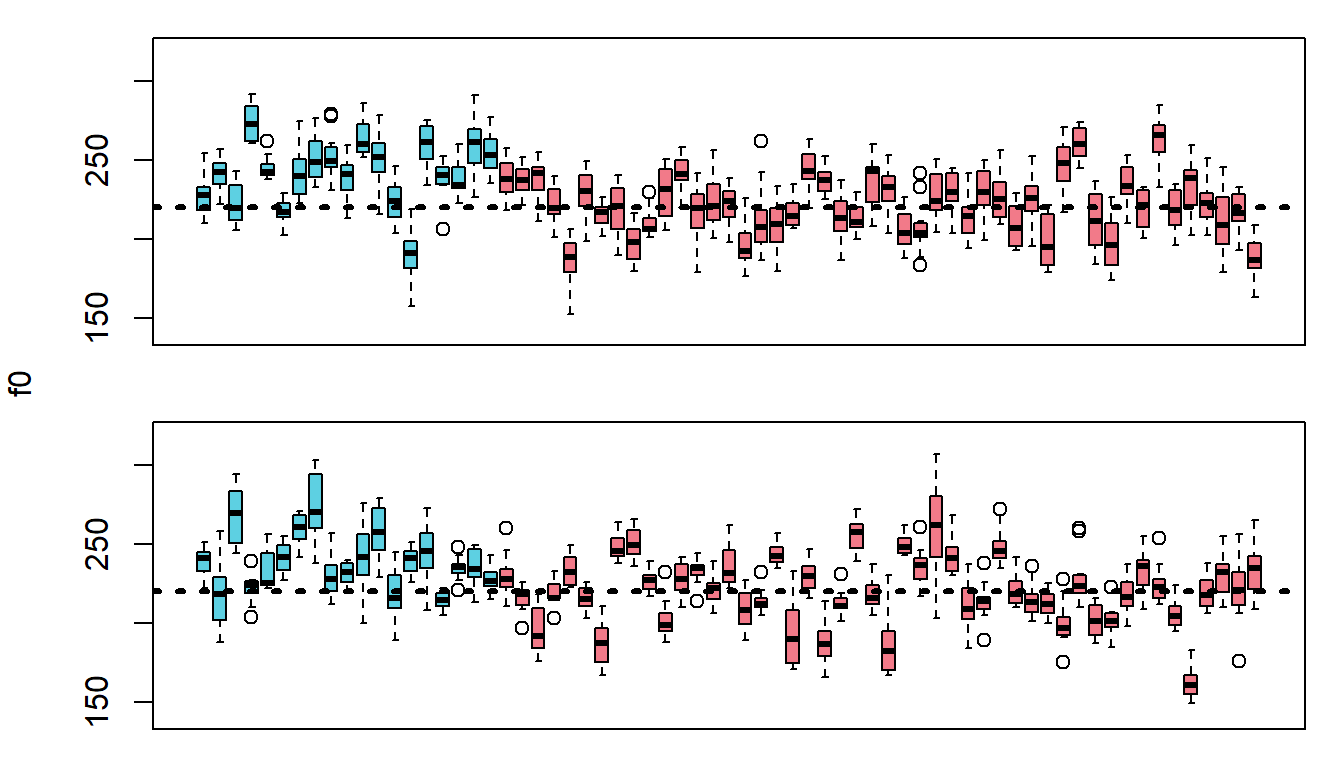
\includegraphics{03_files/figure-latex/F3-simulated-1.pdf}
\caption{\label{fig:F3-simulated}Comparison of real and simulated f0 production data for girls (cyan) and women (red).}
\end{figure}

Below I make three datasets that are `incomplete': the first contains the intercept and noise only, the second contains the intercept and adultness effects only, and the third contains the intercept and speaker effects.

\begin{Shaded}
\begin{Highlighting}[]
\CommentTok{\# only intercept and error}
\NormalTok{f0\_rep\_1 }\OtherTok{=}\NormalTok{ Intercept }\SpecialCharTok{+}\NormalTok{ epsilon}
\CommentTok{\# only intercept and adultness}
\NormalTok{f0\_rep\_2 }\OtherTok{=}\NormalTok{ Intercept }\SpecialCharTok{+}\NormalTok{ adult\_effect[adult]}
\CommentTok{\# only intercept and speaker}
\NormalTok{f0\_rep\_3 }\OtherTok{=}\NormalTok{ Intercept }\SpecialCharTok{+}\NormalTok{ alpha\_speaker[speaker]}
\end{Highlighting}
\end{Shaded}

In the figure below, I compare these `incomplete' datasets to show the contribution that each makes to our data. Notice that the random error variation and speaker variation are centered on the intercept, rather than being affected by the adultness effect.

\begin{figure}
\centering
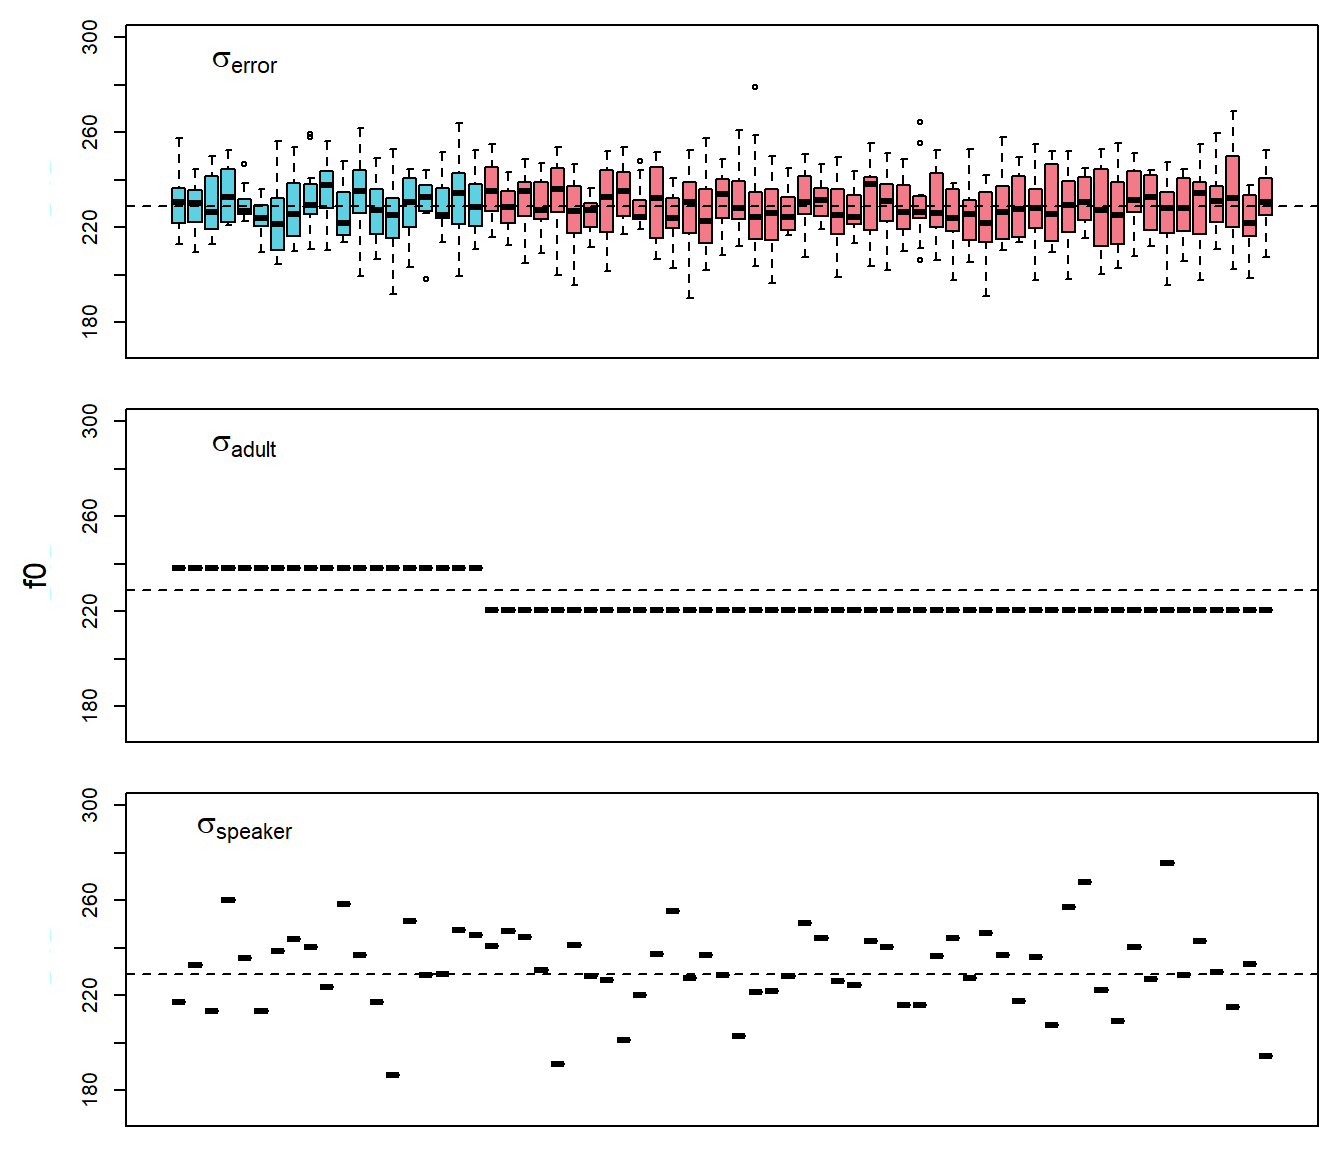
\includegraphics{03_files/figure-latex/F3-sim-incomplete-1-1.pdf}
\caption{\label{fig:F3-sim-incomplete-1}(top) Simulated error variation around the intercept. (middle) Simulated variation according to adultness, but no production error or speaker differences. (bottom) Simulated between-speaker variation, but no production error or adultness effects.}
\end{figure}

Below we can make a few more datasets that mix more components, and compare these to our final simulated data. In each of the datasets shown in these figures, we can see what each source of variance contributes to the data by seeing how the figures change when the source is omitted from the replicated data.

\begin{Shaded}
\begin{Highlighting}[]
\CommentTok{\# intercept, adultness and error}
\NormalTok{f0\_rep\_4 }\OtherTok{=}\NormalTok{ Intercept }\SpecialCharTok{+}\NormalTok{ adult\_effect[adult] }\SpecialCharTok{+}\NormalTok{ epsilon}
\CommentTok{\# intercept, adutlness and speaker}
\NormalTok{f0\_rep\_5 }\OtherTok{=}\NormalTok{ Intercept }\SpecialCharTok{+}\NormalTok{ adult\_effect[adult] }\SpecialCharTok{+}\NormalTok{ alpha\_speaker[speaker]}
\end{Highlighting}
\end{Shaded}

\begin{figure}
\centering
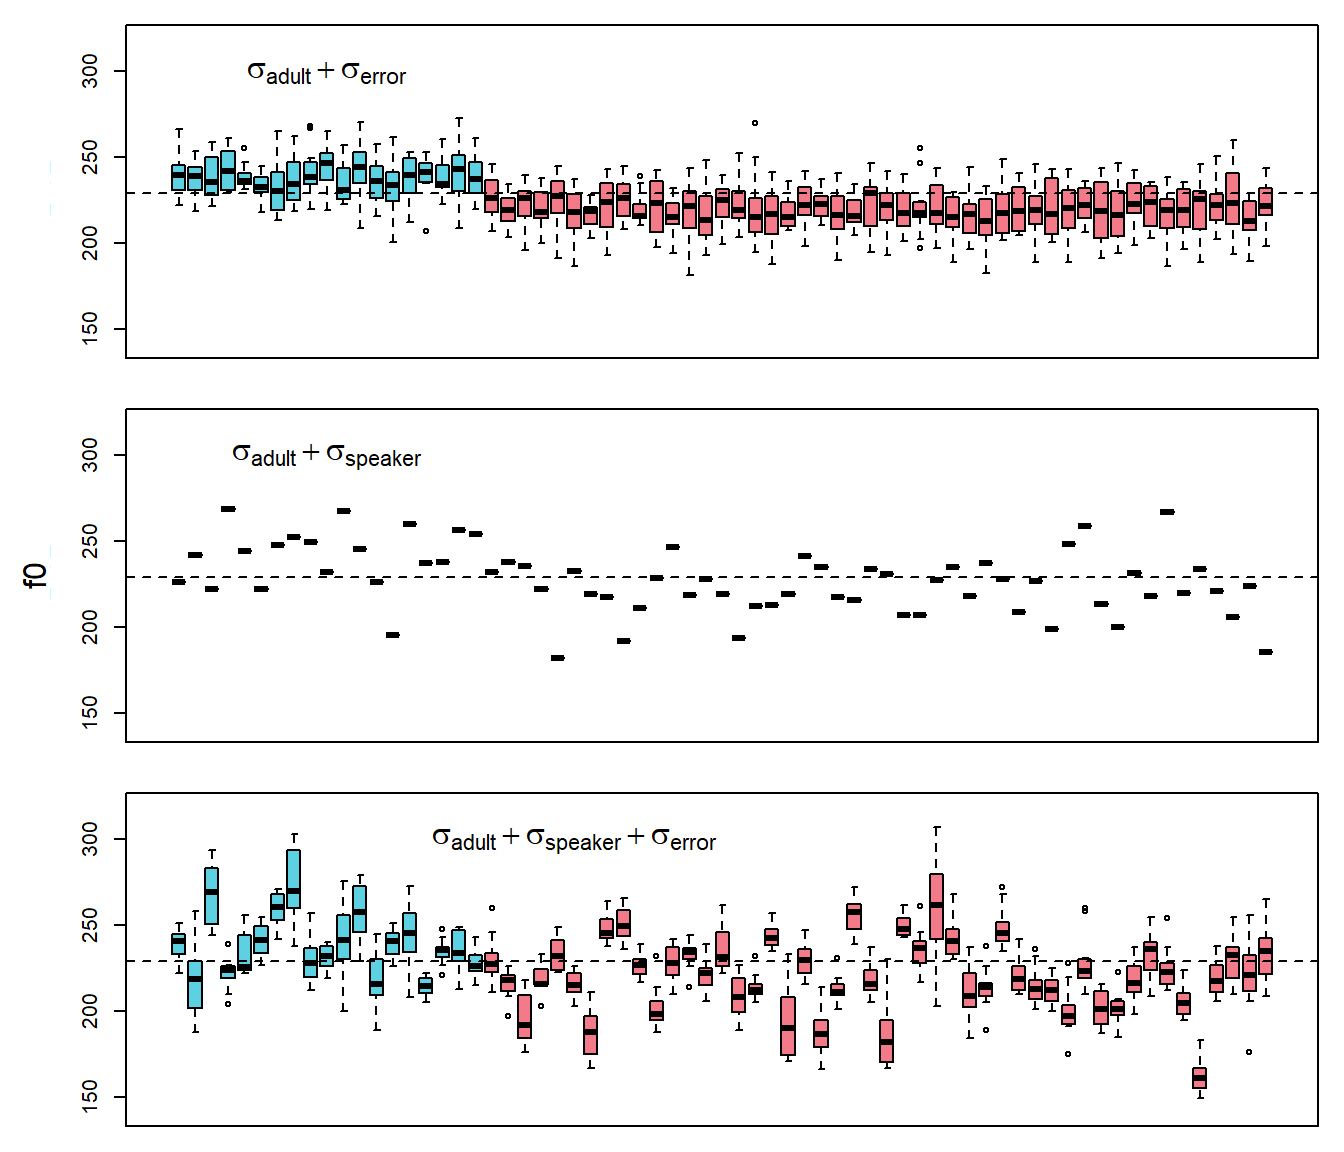
\includegraphics{03_files/figure-latex/F3-sim-incomplete-2-1.pdf}
\caption{\label{fig:F3-sim-incomplete-2}(top) Combination of error variation and effect for adultness. (middle) Combination of between-speaker variation and effect for adultness, but no production error. (bottom) Simulated data containing within and between-speaker variation in f0, in addition to the effects of adultness.}
\end{figure}

\hypertarget{frequentist-corner-1}{%
\section{Frequentist corner}\label{frequentist-corner-1}}

\hypertarget{lmer-corner}{%
\section{Lmer corner}\label{lmer-corner}}

Here I compare the output of \texttt{brms} to the output of the \texttt{lmer} (``linear mixed-effects regression'') function, a very popular function for fitting multilevel models in the lme4 R package. As before, I am not going to talk about the traditional models in any detail. The focus of this section is simply to highlight the potential similarities between different approaches, and to point out where to find this information.

Below I fit a model that is analogous to our \texttt{model\_sum\_coding} model.

\begin{Shaded}
\begin{Highlighting}[]
\FunctionTok{library}\NormalTok{ (lme4)}
\FunctionTok{set.seed}\NormalTok{ (}\DecValTok{1}\NormalTok{)}
\NormalTok{lmer\_model }\OtherTok{=} \FunctionTok{lmer}\NormalTok{ (f0 }\SpecialCharTok{\textasciitilde{}}\NormalTok{ adult }\SpecialCharTok{+}\NormalTok{ (}\DecValTok{1}\SpecialCharTok{|}\NormalTok{speaker), }\AttributeTok{data =}\NormalTok{ females)}

\FunctionTok{summary}\NormalTok{ (lmer\_model)}
\DocumentationTok{\#\# Linear mixed model fit by REML [\textquotesingle{}lmerMod\textquotesingle{}]}
\DocumentationTok{\#\# Formula: f0 \textasciitilde{} adult + (1 | speaker)}
\DocumentationTok{\#\#    Data: females}
\DocumentationTok{\#\# }
\DocumentationTok{\#\# REML criterion at convergence: 6606.9}
\DocumentationTok{\#\# }
\DocumentationTok{\#\# Scaled residuals: }
\DocumentationTok{\#\#     Min      1Q  Median      3Q     Max }
\DocumentationTok{\#\# {-}4.2253 {-}0.5862 {-}0.0669  0.5028  3.8205 }
\DocumentationTok{\#\# }
\DocumentationTok{\#\# Random effects:}
\DocumentationTok{\#\#  Groups   Name        Variance Std.Dev.}
\DocumentationTok{\#\#  speaker  (Intercept) 353.2    18.79   }
\DocumentationTok{\#\#  Residual             167.1    12.93   }
\DocumentationTok{\#\# Number of obs: 804, groups:  speaker, 67}
\DocumentationTok{\#\# }
\DocumentationTok{\#\# Fixed effects:}
\DocumentationTok{\#\#             Estimate Std. Error t value}
\DocumentationTok{\#\# (Intercept)  229.376      2.597  88.335}
\DocumentationTok{\#\# adult1        {-}8.975      2.597  {-}3.456}
\DocumentationTok{\#\# }
\DocumentationTok{\#\# Correlation of Fixed Effects:}
\DocumentationTok{\#\#        (Intr)}
\DocumentationTok{\#\# adult1 {-}0.433}
\end{Highlighting}
\end{Shaded}

We can see that this contains estimates that are very similar to those of our model. The `fixed' effects above correspond closely to their `Population-Level' counterparts.

\begin{Shaded}
\begin{Highlighting}[]
\DocumentationTok{\#\# Population{-}Level Effects: }
\DocumentationTok{\#\#           Estimate Est.Error l{-}95\% CI u{-}95\% CI Rhat Bulk\_ESS Tail\_ESS}
\DocumentationTok{\#\# Intercept   229.33      2.71   224.07   234.81 1.00     2169     2758}
\DocumentationTok{\#\# adult1       {-}8.89      2.65   {-}14.19    {-}3.55 1.00     2085     2825}
\end{Highlighting}
\end{Shaded}

Now that we've talked about random effects in \texttt{brms}, we can pull these out of our \texttt{brm} model and compare them to the random effects we get from \texttt{lmer}.

As seen below, the random effects estimates we get from \texttt{brm} also include credible intervals. As a result, we have some idea regarding the uncertainty in these estimates. Also, since each parameter is estimated by a series of samples, we can compare any two parameters (or groups of parameters) to see how different they are.

\begin{Shaded}
\begin{Highlighting}[]
\NormalTok{brms\_ranefs }\OtherTok{=}\NormalTok{ brms}\SpecialCharTok{::}\FunctionTok{ranef}\NormalTok{ (model\_sum\_coding)}\SpecialCharTok{$}\NormalTok{speaker[,,}\StringTok{"Intercept"}\NormalTok{]}

\FunctionTok{head}\NormalTok{ (brms\_ranefs)}
\DocumentationTok{\#\#      Estimate Est.Error       Q2.5     Q97.5}
\DocumentationTok{\#\# 28   1.184333  5.735588 {-}10.186326 12.319648}
\DocumentationTok{\#\# 29 {-}19.671885  5.652084 {-}30.928433 {-}8.422325}
\DocumentationTok{\#\# 30  28.536109  5.699914  17.484917 39.532266}
\DocumentationTok{\#\# 31 {-}14.595541  5.644469 {-}25.588406 {-}3.446464}
\DocumentationTok{\#\# 32  {-}4.510115  5.729995 {-}15.798335  6.980625}
\DocumentationTok{\#\# 33   2.628343  5.700041  {-}8.534003 13.893796}
\end{Highlighting}
\end{Shaded}

In contrast, \texttt{lmer} gives you what are called \emph{point estimates}. These are single estimates of parameter values with no intervals indicating uncertainty. Because of this, we can't really say to much about these values, nor is there any way to compare the estimates for different speakers/participants in the data.

\begin{Shaded}
\begin{Highlighting}[]
\NormalTok{lmer\_ranefs }\OtherTok{=}\NormalTok{ lme4}\SpecialCharTok{::}\FunctionTok{ranef}\NormalTok{ (lmer\_model)[[}\StringTok{"speaker"}\NormalTok{]]}

\FunctionTok{head}\NormalTok{ (lmer\_ranefs)}
\DocumentationTok{\#\#    (Intercept)}
\DocumentationTok{\#\# 28   0.9451951}
\DocumentationTok{\#\# 29 {-}19.8195602}
\DocumentationTok{\#\# 30  28.4444657}
\DocumentationTok{\#\# 31 {-}14.7686738}
\DocumentationTok{\#\# 32  {-}4.6669009}
\DocumentationTok{\#\# 33   2.5486511}
\end{Highlighting}
\end{Shaded}

Importantly however, the values we get from both approaches are nearly identical, as seen below. The average absolute difference between the two sets of parameters was only 0.08 Hz, and the \emph{largest} difference between the two is 0.25 Hz. So, analyzing this data using a Bayesian multilevel model provides several advantages, while still providing effectively the same `answers' as a `frequentist' approach to the data.

\begin{figure}
\centering
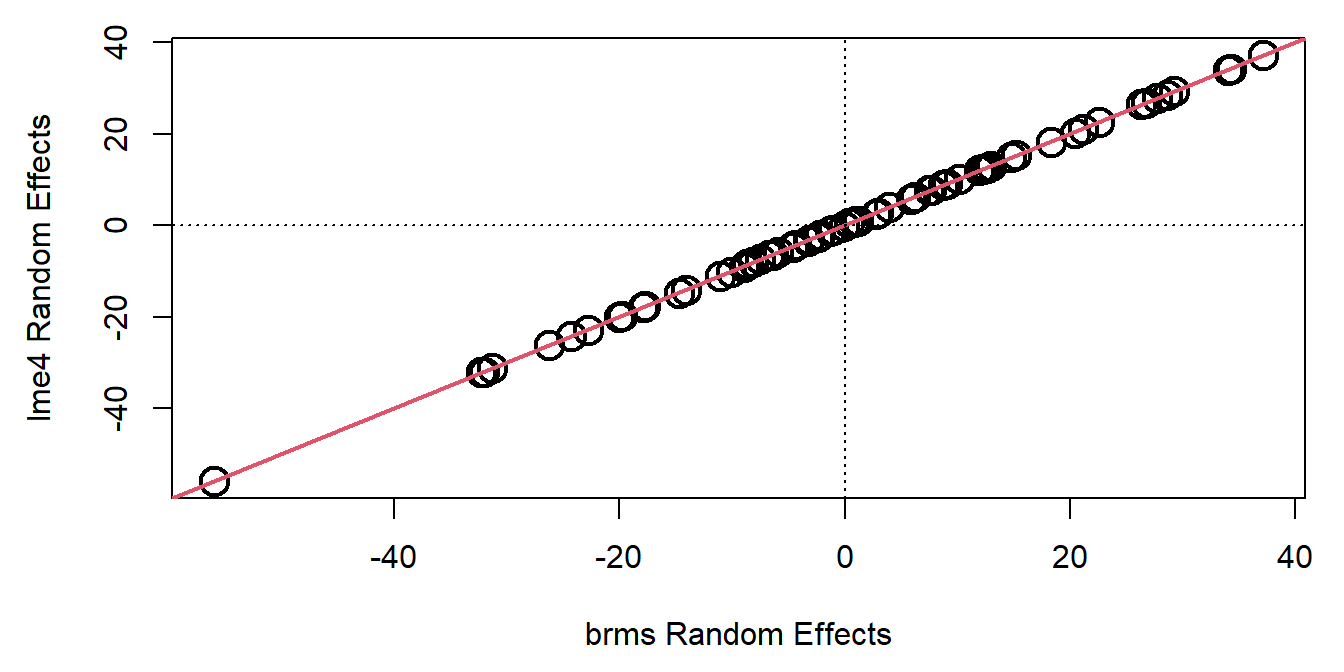
\includegraphics{03_files/figure-latex/unnamed-chunk-30-1.pdf}
\caption{\label{fig:unnamed-chunk-30} (left) In green, the random speaker intercept estimates provided by brm. The red arrows indicate the estimates of the same provided by lmer. .}
\end{figure}

\hypertarget{exercises-2}{%
\section{Exercises}\label{exercises-2}}

\begin{enumerate}
\def\labelenumi{\arabic{enumi})}
\item
  Use the code below to analyze the differences in f0 between the men and boys in the Hillenbrand et al.~data. See if you can get all of the same information out of the model that we considered above. Make a plots of this new data using the plot code provided.
\item
  See if you can use the information from your new data to update the simulated data created above. This entails finding the intercept, the effect for adultness, within-speaker, and between-speaker variation estimates in your new data and using this to generate a new batch of fake/replicated data.
\item
  Use the code below to fit the model below to your own data. Remember, this data should come two group of speakers/participants who each produce one or more data points. You will need to change \texttt{f0}, \texttt{adult}, and \texttt{speaker} in the model below to match the names of the columns containing this information in your data. You may also need to change the priors based on the ranges of your variables. As noted in the last chapter, if in doubt, you can just set all the priors to have means of 0 and standard deviations of 10,000 for now. We will talk about priors in more detail later.
\end{enumerate}

\begin{Shaded}
\begin{Highlighting}[]
\NormalTok{url1 }\OtherTok{=} \StringTok{"https://raw.githubusercontent.com/santiagobarreda/stats{-}class/master/data/"}
\NormalTok{males }\OtherTok{=} \FunctionTok{read.csv}\NormalTok{ (}\FunctionTok{url}\NormalTok{(}\FunctionTok{paste0}\NormalTok{ (url1, }\StringTok{"03\_h95\_vowel\_data\_males.csv"}\NormalTok{)))}

\CommentTok{\# set contrasts}
\FunctionTok{options}\NormalTok{ (}\AttributeTok{contrasts =} \FunctionTok{c}\NormalTok{(}\StringTok{\textquotesingle{}contr.sum\textquotesingle{}}\NormalTok{,}\StringTok{\textquotesingle{}contr.sum\textquotesingle{}}\NormalTok{))}

\FunctionTok{set.seed}\NormalTok{ (}\DecValTok{1}\NormalTok{)}
\NormalTok{excercise\_model }\OtherTok{=}  
\NormalTok{  brms}\SpecialCharTok{::}\FunctionTok{brm}\NormalTok{ (f0 }\SpecialCharTok{\textasciitilde{}}\NormalTok{ adult }\SpecialCharTok{+}\NormalTok{ (}\DecValTok{1}\SpecialCharTok{|}\NormalTok{speaker), }\AttributeTok{data =}\NormalTok{ males, }\AttributeTok{chains =} \DecValTok{4}\NormalTok{, }\AttributeTok{cores =} \DecValTok{4}\NormalTok{,}
       \AttributeTok{warmup =} \DecValTok{1000}\NormalTok{, }\AttributeTok{iter =} \DecValTok{11000}\NormalTok{, }\AttributeTok{thin =} \DecValTok{10}\NormalTok{,}
       \AttributeTok{prior =} \FunctionTok{c}\NormalTok{(}\FunctionTok{set\_prior}\NormalTok{(}\StringTok{"student\_t(3, 220, 100)"}\NormalTok{, }\AttributeTok{class =} \StringTok{"Intercept"}\NormalTok{),}
                 \FunctionTok{set\_prior}\NormalTok{(}\StringTok{"student\_t(3, 0, 100)"}\NormalTok{, }\AttributeTok{class =} \StringTok{"b"}\NormalTok{),}
                 \FunctionTok{set\_prior}\NormalTok{(}\StringTok{"student\_t(3, 0, 100)"}\NormalTok{, }\AttributeTok{class =} \StringTok{"sd"}\NormalTok{),}
                 \FunctionTok{set\_prior}\NormalTok{(}\StringTok{"student\_t(3, 0, 100)"}\NormalTok{, }\AttributeTok{class =} \StringTok{"sigma"}\NormalTok{)))}
\end{Highlighting}
\end{Shaded}

\begin{Shaded}
\begin{Highlighting}[]
\NormalTok{url1 }\OtherTok{=} \StringTok{"https://raw.githubusercontent.com/santiagobarreda"}
\NormalTok{url2 }\OtherTok{=} \StringTok{"/stats{-}class/master/data/h95\_vowel\_data.csv"}
\CommentTok{\# set up colors for plotting}
\NormalTok{devtools}\SpecialCharTok{::}\FunctionTok{source\_url}\NormalTok{ (}\FunctionTok{paste0}\NormalTok{ (url1, }\StringTok{"/stats{-}class/master/data/colors.R"}\NormalTok{))}
\CommentTok{\# source functions}
\NormalTok{devtools}\SpecialCharTok{::}\FunctionTok{source\_url}\NormalTok{ (}\FunctionTok{paste0}\NormalTok{ (url1, }\StringTok{"/stats{-}class/master/data/functions.R"}\NormalTok{))}

\NormalTok{url1 }\OtherTok{=} \StringTok{"https://raw.githubusercontent.com/santiagobarreda/stats{-}class/master/data/"}
\NormalTok{h95 }\OtherTok{=} \FunctionTok{read.csv}\NormalTok{ (}\FunctionTok{url}\NormalTok{(}\FunctionTok{paste0}\NormalTok{ (url1, }\StringTok{"03\_h95\_vowel\_data.csv"}\NormalTok{)))}
\end{Highlighting}
\end{Shaded}

\hypertarget{comparing-many-groups}{%
\chapter{Comparing many groups}\label{comparing-many-groups}}

Last chapter we talked about comparing two groups. Although the comparison of two groups is very simple, it also comes up very often: more complicated problems are often broken down into several two-group questions. However, most real-world research designs don't usually \emph{begin} as two-group questions. In this chapter, we're going to talk about the comparison of multiple groups of observations/speakers.

The models discussed in this chapter can be used for data that compares observations across any number of groups. Again, we're using the term `groups' loosely here. The designs in this chapter are appropriate for data from:

\begin{itemize}
\item
  groups of speakers/listeners that are grouped in different ways because they differ in some characteristic (e.g., first language), or in some experimental condition. Different speakers are in each group.
\item
  the same speakers/listeners are tested in multiple different experimental condition, with stimuli that vary in multiple groups, or something of the sort.
\item
  each speaker/subject can contribute multiple data points, and the number does not need to be balanced across subjects. Also speakers can be missing from one of the conditions (i.e., unbalanced data is ok).
\end{itemize}

The models we will discuss are similar to one-way ANOVAs in the types of research questions they can help investigate.

\hypertarget{data-and-research-questions-3}{%
\section{Data and research questions}\label{data-and-research-questions-3}}

We're going to keep working with the Hillenbrand et al.~data, that we have been discussing in every chapter to this point. This time we're going to work with all four groups of speakers: \texttt{b} (boys), \texttt{g} (girls), \texttt{m} (men), and \texttt{w} (women).

\begin{Shaded}
\begin{Highlighting}[]
\CommentTok{\# load brms}
\FunctionTok{library}\NormalTok{ (brms)}
\CommentTok{\# load data from course website}
\NormalTok{url1 }\OtherTok{=} \StringTok{"https://raw.githubusercontent.com/santiagobarreda/stats{-}class/master/data/"}
\NormalTok{h95 }\OtherTok{=} \FunctionTok{read.csv}\NormalTok{ (}\FunctionTok{url}\NormalTok{(}\FunctionTok{paste0}\NormalTok{ (url1, }\StringTok{"03\_h95\_vowel\_data.csv"}\NormalTok{)))}
\end{Highlighting}
\end{Shaded}

Our potential research questions are substantially more complicated than in the two-group case. First, there are four groups now, meaning we could potentially make 6 2-group comparisons. Second, the groups differ along multiple dimensions, making it more difficult to make two-group comparisons that ask one single question. For example, the `man' and `girl' groups differ according to `adultness' \emph{and} `gender.' How could we know what part of their f0 difference we should attribute to adultness and what part we should attribute to maleness?

\begin{figure}
\centering
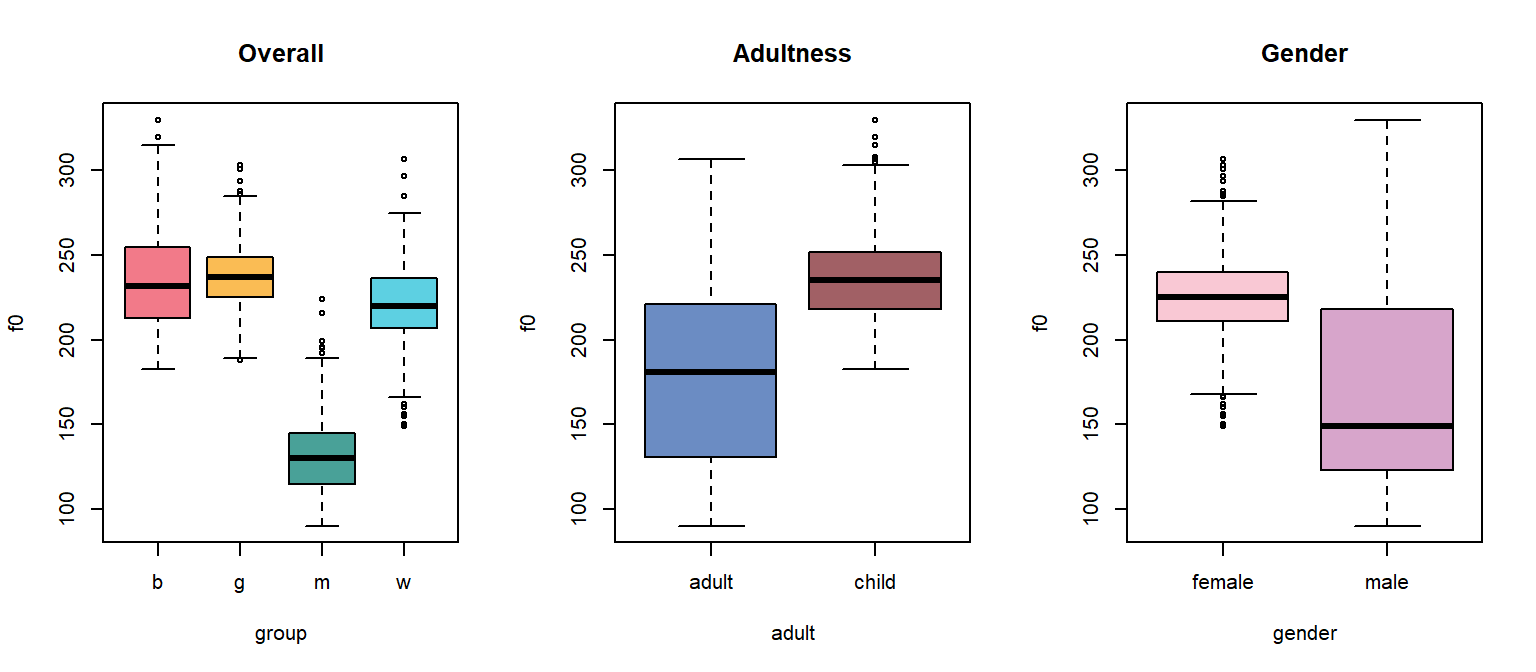
\includegraphics{04_files/figure-latex/F4-datacomparison-1.pdf}
\caption{\label{fig:F4-datacomparison}(left) Comparison of the four groups (middle) Comparison of productions based on whether the speaker is an adult (right) Comparison of all productions based on whether the speaker is male.}
\end{figure}

We can consider our data in several ways: as four independent groups, or as two 2-groups comparisons (adult vs child, female vs male). We're going to focus on the 4-way comparison first, and later talk about models that make multiple comparisons simultaneously.

\begin{figure}
\centering
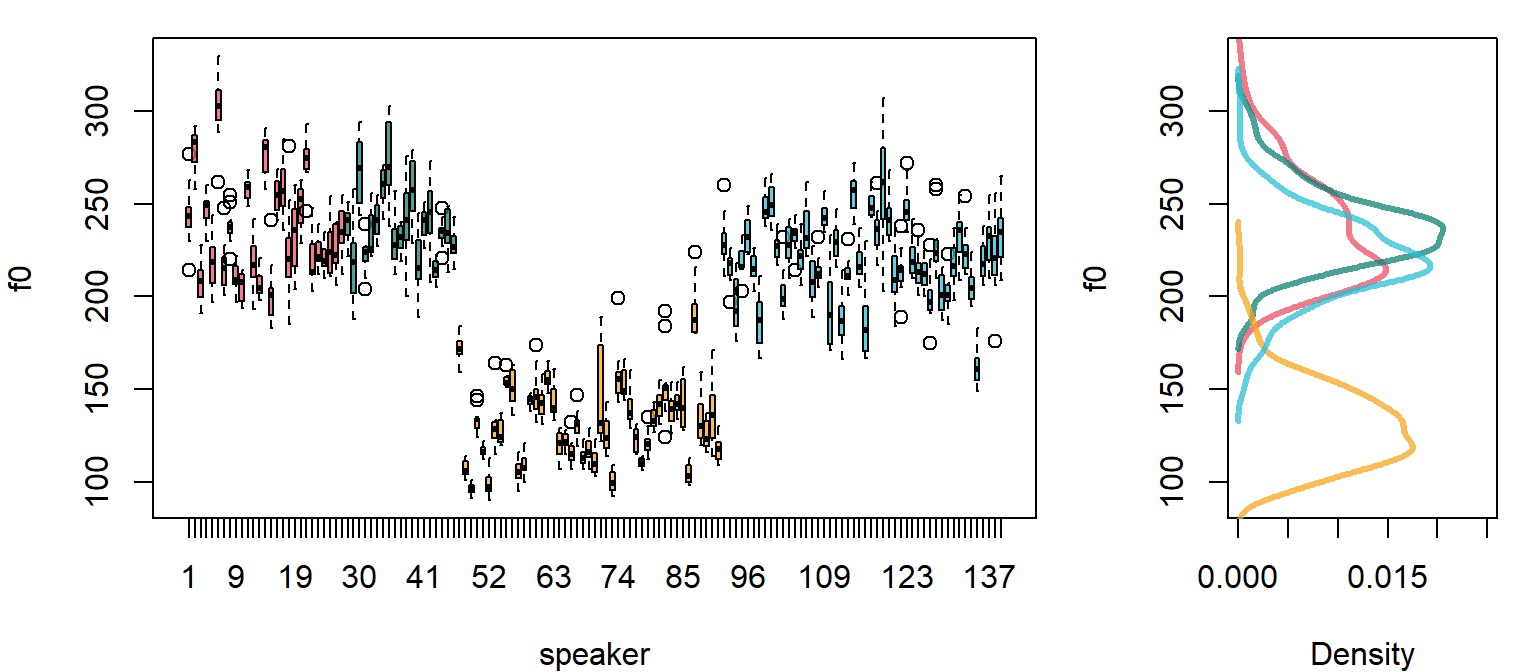
\includegraphics{04_files/figure-latex/F4-speakerboxplots-1.pdf}
\caption{\label{fig:F4-speakerboxplots}(left) Boxplots presenting each speaker's production of f0 for boys (red), girls (yellow), men (green), and women (teal). (right) Densities of the overall distributions for each group.}
\end{figure}

\hypertarget{factors-as-batches-effects}{%
\subsection{Factors as `batches' effects}\label{factors-as-batches-effects}}

R treats nominal, categorical predictors as \emph{factors} and assumes that each different label is a different group. Each group of a factor is called a \emph{level}. Actually, we've been using factors all along because our \texttt{speaker} predictor is a factor and the individual participants are levels! As far as our models are concerned, participant/speaker/subject has no special status as a predictor and it is just a factor with many levels.

When you have groups in your model that are `thematically' related, you can `batch' them together in a factor. For example you may have 4 groups of speakers based on native language. You can treat these four groups as levels of a factor. Implicitly, this tells your model that these four groups are related somehow. You know that they are related by being first language groups. However, keep in mind your model `knows' next to nothing. Actually, the way you tell your model that these groups are related is precisely by treating them as levels of the same factor rather than as unrelated groups.

For example, the same speakers might be divided into women and men. This would introduce two new levels into our design. However, should we just through men and women into the language factor: Italians, Germans, English, Russians, Men and Women? We could definitely do this, no one ill stop us. But this doesn't make much \emph{sense}. Instead, it makes sense to split these groups into two batches of levels: one factor with four language levels, and one factor with two gender levels.

A \texttt{factor} is actually a data type in R. It's basically the same as a vector of words (or numbers!), but it has some additional properties that are useful. For example, consider our \texttt{group} predictor, which tells us which group each speaker falls into. Initially it is a character vector. We see that the first few tokens are produced by men (\texttt{m}), and that there is no numerical value associated with these letter labels. The \texttt{unique} function returns all unique labels in the vector, in the order that they appear in the vector.

\begin{Shaded}
\begin{Highlighting}[]
\CommentTok{\# see the first 6 observations}
\FunctionTok{head}\NormalTok{ (h95}\SpecialCharTok{$}\NormalTok{group)   }
\DocumentationTok{\#\# [1] "b" "b" "b" "b" "b" "b"}

\CommentTok{\# class starts as a character vector}
\FunctionTok{class}\NormalTok{ (h95}\SpecialCharTok{$}\NormalTok{group)   }
\DocumentationTok{\#\# [1] "character"}

\CommentTok{\# no numerical values}
\FunctionTok{head}\NormalTok{ (}\FunctionTok{as.numeric}\NormalTok{ (h95}\SpecialCharTok{$}\NormalTok{group))  }
\DocumentationTok{\#\# Warning in head(as.numeric(h95$group)): NAs introduced by coercion}
\DocumentationTok{\#\# [1] NA NA NA NA NA NA}

\CommentTok{\# we can see the number of unique groups}
\FunctionTok{unique}\NormalTok{ (h95}\SpecialCharTok{$}\NormalTok{group)  }
\DocumentationTok{\#\# [1] "b" "g" "m" "w"}
\end{Highlighting}
\end{Shaded}

We can turn the character vector \texttt{group} into a factor vector \texttt{group\_f}. The benefit of this is that these nominal labels now have an inherent ordering, and associated numerical values. R functions such as \texttt{brm} turn your nominal (non-numeric) predictors into factors in the process of fitting the model. Doing this yourself gives you control over how they will be handled.

\begin{Shaded}
\begin{Highlighting}[]
\CommentTok{\# we can turn it into a factor in R}
\NormalTok{h95}\SpecialCharTok{$}\NormalTok{group\_f }\OtherTok{=} \FunctionTok{factor}\NormalTok{(h95}\SpecialCharTok{$}\NormalTok{group) }

\CommentTok{\# now it has official levels}
\FunctionTok{levels}\NormalTok{(h95}\SpecialCharTok{$}\NormalTok{group\_f)  }
\DocumentationTok{\#\# [1] "b" "g" "m" "w"}

\CommentTok{\# now it has nuerical values}
\FunctionTok{head}\NormalTok{ (}\FunctionTok{as.numeric}\NormalTok{ (h95}\SpecialCharTok{$}\NormalTok{group\_f))  }
\DocumentationTok{\#\# [1] 1 1 1 1 1 1}
\end{Highlighting}
\end{Shaded}

By default factor levels are ordered alphabetically. This means that if we are using sum coding we omit the \texttt{w} parameter (the `last group') and if we are using treatment coding, the intercept will be equal to \texttt{m} (the `first' group). You can control this behavior by re-ordering the factor levels as below:

\begin{Shaded}
\begin{Highlighting}[]
\NormalTok{h95}\SpecialCharTok{$}\NormalTok{group\_f2 }\OtherTok{=} \FunctionTok{factor}\NormalTok{ (h95}\SpecialCharTok{$}\NormalTok{group\_f, }\AttributeTok{levels =} \FunctionTok{c}\NormalTok{(}\StringTok{\textquotesingle{}w\textquotesingle{}}\NormalTok{,}\StringTok{\textquotesingle{}m\textquotesingle{}}\NormalTok{,}\StringTok{\textquotesingle{}g\textquotesingle{}}\NormalTok{,}\StringTok{\textquotesingle{}b\textquotesingle{}}\NormalTok{))}

\FunctionTok{levels}\NormalTok{ (h95}\SpecialCharTok{$}\NormalTok{group\_f2)}
\DocumentationTok{\#\# [1] "w" "m" "g" "b"}

\CommentTok{\# note that \textquotesingle{}m\textquotesingle{} is now the second category}
\FunctionTok{head}\NormalTok{ (}\FunctionTok{as.numeric}\NormalTok{ (h95}\SpecialCharTok{$}\NormalTok{group\_f2))  }
\DocumentationTok{\#\# [1] 4 4 4 4 4 4}
\end{Highlighting}
\end{Shaded}

After this reordering, we would omit the (last) \texttt{b} parameter under sum coding, and under treatment coding the first group (\texttt{w}) would be equal to the intercept.

In general, representing all groups requires about one variable per group. Our single predictor, \texttt{group}, has four levels: \texttt{b},\texttt{g},\texttt{m}, and \texttt{w}. For models where the predictor is a factor with more than two levels, we can represent the predictor in a vector like this, \(group_{[i]}\), where \(i\) is a counter variable that goes from 1 to the number of groups.

So the group effects can be represented in a vector as below, representing the effects (deviations from the intercept) for boys, girls, men and women:

\begin{Shaded}
\begin{Highlighting}[]
\FunctionTok{c}\NormalTok{(}\DecValTok{30}\NormalTok{, }\DecValTok{32}\NormalTok{, }\SpecialCharTok{{-}}\DecValTok{75}\NormalTok{, }\DecValTok{13}\NormalTok{)}
\DocumentationTok{\#\# [1]  30  32 {-}75  13}
\end{Highlighting}
\end{Shaded}

We can then make a short factor vector with the same labels used in this experiment. Below we can see the sequence of letter labels I specified, and their corresponding numeric values (based on alphabetical ordering).

\begin{Shaded}
\begin{Highlighting}[]
\NormalTok{group\_index }\OtherTok{=} \FunctionTok{factor}\NormalTok{ (}\FunctionTok{c}\NormalTok{(}\StringTok{\textquotesingle{}b\textquotesingle{}}\NormalTok{,}\StringTok{\textquotesingle{}w\textquotesingle{}}\NormalTok{,}\StringTok{\textquotesingle{}m\textquotesingle{}}\NormalTok{,}\StringTok{\textquotesingle{}w\textquotesingle{}}\NormalTok{,}\StringTok{\textquotesingle{}g\textquotesingle{}}\NormalTok{))}

\FunctionTok{data.frame}\NormalTok{ (group\_index, }\AttributeTok{group\_index\_number =} \FunctionTok{as.numeric}\NormalTok{ (group\_index))}
\DocumentationTok{\#\#   group\_index group\_index\_number}
\DocumentationTok{\#\# 1           b                  1}
\DocumentationTok{\#\# 2           w                  4}
\DocumentationTok{\#\# 3           m                  3}
\DocumentationTok{\#\# 4           w                  4}
\DocumentationTok{\#\# 5           g                  2}
\end{Highlighting}
\end{Shaded}

We can then take this vector of factor levels and use it to generate a sequence of effects:

\begin{Shaded}
\begin{Highlighting}[]
\FunctionTok{as.numeric}\NormalTok{ (group\_index)}
\DocumentationTok{\#\# [1] 1 4 3 4 2}

\FunctionTok{c}\NormalTok{(}\DecValTok{30}\NormalTok{, }\DecValTok{32}\NormalTok{, }\SpecialCharTok{{-}}\DecValTok{75}\NormalTok{, }\DecValTok{13}\NormalTok{)[group\_index]}
\DocumentationTok{\#\# [1]  30  13 {-}75  13  32}
\end{Highlighting}
\end{Shaded}

Notice that the sequence of effects match the sequence of group levels, based on their numerical value.

If every single group were to get an independent parameter represented in our regression equation, these would become very long and difficult to interpret. Instead, by treating the effects for the level of a factor as a vector, our models can represent a very large number of parameters in a concise way. For example, compare the following two possible implementations of our 4 group model (where \(j\) is an index for our group effects):

\begin{equation}
\begin{split}
\mu_{[i]} = Intercept + group_{[1]} + group_{[2]} + group_{[3]} + group_{[4]} \\
\mu_{[i]} = Intercept + group_{[j]} \\
\end{split}
\label{eq:40}
\end{equation}

It may seem like too much of a difference now, but later we have have many factors, some with dozens or hundreds of levels. In those cases, representing factor effects using vectors becomes essential.

\hypertarget{comparing-four-or-any-number-of-groups}{%
\section{Comparing four (or any number of) groups}\label{comparing-four-or-any-number-of-groups}}

We're first going to treat the four groups as if they had no internal structure. In this case it may not be the best approach for this data, since we know there are logical ways to subdivide men, women, boys and girls. However, this is a good starting point since many cases you will have several groups with no logical internal divisions.

\hypertarget{the-model}{%
\subsection{The model}\label{the-model}}

Our updated model is now:

\begin{equation}
\begin{split}
\textrm{Likelihood:} \\
y_{[i]} \sim \mathcal{N}(\mu_{[i]},\sigma_{error}) \\
\mu_{[i]} = Intercept + group_{[\mathrm{group}_{[i]}]} + \alpha_{[speaker_{[i]}]} \\\\
\textrm{Priors:} \\
\alpha_{[speaker]} \sim \mathcal{N}(0,\sigma_{[speaker]}) \\ \\ 
Intercept \sim t(3, 220, 100) \\ 
group_{[\mathrm{group}]} \sim t(3, 0, 100) \\ 
\sigma_{error} \sim t(3, 0, 100) \\
\sigma_{speaker} \sim t(3, 0, 100) \\ 
\end{split}
\label{eq:41}
\end{equation}

Notice that for each trial number \(i\) the group predictor is indexed by a variable called \texttt{group}. This is a bit confusing, but I am just trying to be consistent with how R does things.

As noted above, a factor predictor like \texttt{group} is really just a bunch of numbers that represent group effects in a vector. So R really treats your \texttt{group} as a sequence of numbers representing group numbers. But it also calls the predictor in the model by that name! So, though it may look strange \(group_{[\mathrm{group}_{[i]}]}\) just says that you have a predictor in your model called \(group\) and it has a few possible values (four in this case). Also, you have a variable in your data with the same name (\texttt{group}) that tells you which value of your \(group\) predictor to use for each observation!

This may sound convoluted, but it is simply what I demonstrated in the end of the last subsection regarding the behavior of vectors and factors. Our model will estimate three \(group\) effects (it must omit one). It estimates these from a the prior distribution specified in the model above (\(group \sim t(3, 0, 100)\)). Our \emph{data} includes a predictor called \texttt{group} that simply tells us which value of our group effect to use in each trial (\texttt{group{[}i{]}} = \(\mathrm{group}_{[i]}\)).

For example, above we saw that the first value of the \texttt{group} vector is 3. This means this speaker is a member of the \texttt{m} group. So, in our model above the equation determining \(\mu_{[i]}\) will include the value \(group_{[3]}\) in it because, for the third observation this predictor will be \(group_{[\mathrm{group}_{[1]}=3]}\).

As in the previous chapters, we fit the models using weakly-informative priors. We're going to use sum coding, which means that the intercept will be the mean of all the groups, and group effects will be represented as differences from this mean. Remember that the missing group effect will be equal to the negative sum of the coefficients that \emph{are} present. By default, R drops the \emph{last} level from your factor, which in our case will be the \texttt{w} level. We can set R to use sum coding with the line below:

\begin{Shaded}
\begin{Highlighting}[]
\FunctionTok{options}\NormalTok{ (}\AttributeTok{contrasts =} \FunctionTok{c}\NormalTok{(}\StringTok{"contr.sum"}\NormalTok{,}\StringTok{"cont.sum"}\NormalTok{))}
\end{Highlighting}
\end{Shaded}

And fit the model below:

\begin{Shaded}
\begin{Highlighting}[]
\FunctionTok{options}\NormalTok{ (}\AttributeTok{contrasts =} \FunctionTok{c}\NormalTok{(}\StringTok{"contr.sum"}\NormalTok{,}\StringTok{"cont.sum"}\NormalTok{))}
\CommentTok{\# Fit the model yourself, or download pre{-}fit model from: }
\CommentTok{\# github.com/santiagobarreda/stats{-}class/tree/master/models}
\CommentTok{\# and load after placing in working directory}
\CommentTok{\#  model\_four\_groups = readRDS (\textquotesingle{}4\_model\_four\_groups.RDS\textquotesingle{})set.seed (1)}

\NormalTok{model\_four\_groups }\OtherTok{=}  
  \FunctionTok{brm}\NormalTok{ (f0 }\SpecialCharTok{\textasciitilde{}}\NormalTok{ group }\SpecialCharTok{+}\NormalTok{ (}\DecValTok{1}\SpecialCharTok{|}\NormalTok{speaker), }\AttributeTok{data =}\NormalTok{ h95, }\AttributeTok{chains =} \DecValTok{4}\NormalTok{, }\AttributeTok{cores =} \DecValTok{4}\NormalTok{, }
       \AttributeTok{warmup =} \DecValTok{1000}\NormalTok{, }\AttributeTok{iter =} \DecValTok{11000}\NormalTok{, }\AttributeTok{thin =} \DecValTok{10}\NormalTok{, }
       \AttributeTok{prior =} \FunctionTok{c}\NormalTok{(}\FunctionTok{set\_prior}\NormalTok{(}\StringTok{"student\_t(3, 200, 100)"}\NormalTok{, }\AttributeTok{class =} \StringTok{"Intercept"}\NormalTok{),}
                              \FunctionTok{set\_prior}\NormalTok{(}\StringTok{"student\_t(3, 0, 100)"}\NormalTok{, }\AttributeTok{class =} \StringTok{"b"}\NormalTok{),}
                              \FunctionTok{set\_prior}\NormalTok{(}\StringTok{"student\_t(3, 0, 100)"}\NormalTok{, }\AttributeTok{class =} \StringTok{"sd"}\NormalTok{)))}

\CommentTok{\#  saveRDS (model\_four\_groups, \textquotesingle{}model\_four\_groups.RDS\textquotesingle{})}
\end{Highlighting}
\end{Shaded}

\begin{Shaded}
\begin{Highlighting}[]
\CommentTok{\# inspect model}
\NormalTok{model\_four\_groups}
\DocumentationTok{\#\#  Family: gaussian }
\DocumentationTok{\#\#   Links: mu = identity; sigma = identity }
\DocumentationTok{\#\# Formula: f0 \textasciitilde{} group + (1 | speaker) }
\DocumentationTok{\#\#    Data: h95 (Number of observations: 1668) }
\DocumentationTok{\#\# Samples: 4 chains, each with iter = 11000; warmup = 1000; thin = 10;}
\DocumentationTok{\#\#          total post{-}warmup samples = 4000}
\DocumentationTok{\#\# }
\DocumentationTok{\#\# Group{-}Level Effects: }
\DocumentationTok{\#\# \textasciitilde{}speaker (Number of levels: 139) }
\DocumentationTok{\#\#               Estimate Est.Error l{-}95\% CI u{-}95\% CI Rhat Bulk\_ESS Tail\_ESS}
\DocumentationTok{\#\# sd(Intercept)    20.95      1.34    18.51    23.82 1.00     2080     2564}
\DocumentationTok{\#\# }
\DocumentationTok{\#\# Population{-}Level Effects: }
\DocumentationTok{\#\#           Estimate Est.Error l{-}95\% CI u{-}95\% CI Rhat Bulk\_ESS Tail\_ESS}
\DocumentationTok{\#\# Intercept   206.49      1.93   202.67   210.21 1.00     1474     2270}
\DocumentationTok{\#\# group1       29.53      3.52    22.78    36.65 1.00     1253     2236}
\DocumentationTok{\#\# group2       31.88      3.98    24.35    39.68 1.00     1565     2392}
\DocumentationTok{\#\# group3      {-}75.18      2.90   {-}80.89   {-}69.62 1.00     1246     2383}
\DocumentationTok{\#\# }
\DocumentationTok{\#\# Family Specific Parameters: }
\DocumentationTok{\#\#       Estimate Est.Error l{-}95\% CI u{-}95\% CI Rhat Bulk\_ESS Tail\_ESS}
\DocumentationTok{\#\# sigma    11.86      0.22    11.46    12.31 1.00     3882     3814}
\DocumentationTok{\#\# }
\DocumentationTok{\#\# Samples were drawn using sampling(NUTS). For each parameter, Bulk\_ESS}
\DocumentationTok{\#\# and Tail\_ESS are effective sample size measures, and Rhat is the potential}
\DocumentationTok{\#\# scale reduction factor on split chains (at convergence, Rhat = 1).}
\end{Highlighting}
\end{Shaded}

We can see that the intercept is the average of the group means, and our coefficients are equal to the centered group means. Notice that we use the hypothesis function to recover the final group coefficient using the negative sum of the coefficients that were estimated.

\begin{Shaded}
\begin{Highlighting}[]
\CommentTok{\# group means}
\NormalTok{means }\OtherTok{=} \FunctionTok{tapply}\NormalTok{ (h95}\SpecialCharTok{$}\NormalTok{f0, h95}\SpecialCharTok{$}\NormalTok{group, mean)}

\CommentTok{\# overall mean}
\FunctionTok{mean}\NormalTok{ (means)}
\DocumentationTok{\#\# [1] 206.5111}

\CommentTok{\# group means}
\NormalTok{means}
\DocumentationTok{\#\#        b        g        m        w }
\DocumentationTok{\#\# 236.0741 238.3509 131.2185 220.4010}

\CommentTok{\# centered means}
\NormalTok{means }\SpecialCharTok{{-}} \FunctionTok{mean}\NormalTok{ (means)}
\DocumentationTok{\#\#         b         g         m         w }
\DocumentationTok{\#\#  29.56295  31.83975 {-}75.29261  13.88991}

\CommentTok{\# parameters = centered means}
\NormalTok{brms}\SpecialCharTok{::}\FunctionTok{hypothesis}\NormalTok{ (model\_four\_groups, }
                  \FunctionTok{c}\NormalTok{(}\StringTok{"Intercept = 0"}\NormalTok{,}
                    \StringTok{"group1 = 0"}\NormalTok{,}
                    \StringTok{"group2 = 0"}\NormalTok{,}
                    \StringTok{"group3 = 0"}\NormalTok{, }
                    \StringTok{"{-}(group1+group2+group3) = 0"}\NormalTok{))[[}\DecValTok{1}\NormalTok{]][,}\DecValTok{1}\SpecialCharTok{:}\DecValTok{5}\NormalTok{]}
\DocumentationTok{\#\#                      Hypothesis  Estimate Est.Error   CI.Lower  CI.Upper}
\DocumentationTok{\#\# 1               (Intercept) = 0 206.48607  1.928704 202.669676 210.21349}
\DocumentationTok{\#\# 2                  (group1) = 0  29.53202  3.523919  22.783088  36.64507}
\DocumentationTok{\#\# 3                  (group2) = 0  31.87791  3.976443  24.351030  39.68355}
\DocumentationTok{\#\# 4                  (group3) = 0 {-}75.17590  2.903665 {-}80.888641 {-}69.61975}
\DocumentationTok{\#\# 5 ({-}(group1+group2+group3)) = 0  13.76598  2.934586   7.923066  19.37857}
\end{Highlighting}
\end{Shaded}

Whn you fit a more traditional model, you can't just compare any groups you want. However, with these Bayesian models we can compare any groups we want by using comparisons of the posterior samples (as shown in chapter 3). For example, the difference between girls and boys can be found by asking if one minus the other equals 0 (which would be true if these were identical):

\begin{Shaded}
\begin{Highlighting}[]
\NormalTok{brms}\SpecialCharTok{::}\FunctionTok{hypothesis}\NormalTok{ (model\_four\_groups, }\StringTok{"group1 {-} group2 = 0"}\NormalTok{)[[}\DecValTok{1}\NormalTok{]][,}\DecValTok{1}\SpecialCharTok{:}\DecValTok{5}\NormalTok{]}
\DocumentationTok{\#\#            Hypothesis  Estimate Est.Error  CI.Lower CI.Upper}
\DocumentationTok{\#\# 1 (group1{-}group2) = 0 {-}2.345888  6.437511 {-}15.03817 10.28229}
\end{Highlighting}
\end{Shaded}

The result above suggests that the difference is very small (-2 Hz) and the 95\% credible intervals spans a huge range (from -15 to +10)). As a result, the measured difference between these groups is not reliable, and may be very small or close to zero. Notice that in this summary I am focused on minimizing \href{https://statmodeling.stat.columbia.edu/2004/12/29/type_1_type_2_t/}{type S and type M errors}. This means I am worried about whether the effect is likely to be small or large, and negative or positive, rather than whether it is `true' or `false'.

\hypertarget{investigating-many-groups-using-predictors-analysis-of-variance}{%
\section{Investigating many groups using predictors: Analysis of Variance}\label{investigating-many-groups-using-predictors-analysis-of-variance}}

\hypertarget{description-of-the-model-3}{%
\subsection{Description of the model}\label{description-of-the-model-3}}

In the previous section, we acted like we just had four different groups with no internal structure. Of course, we know that our groups differ systematically from each other in meaningful ways. For example, we might have chosen to fit two separate models that looked like this:

\texttt{brm\ (f0\ \textasciitilde{}\ gender\ +\ (1\textbar{}speaker)}

\texttt{brm\ (f0\ \textasciitilde{}\ adult\ +\ (1\textbar{}speaker)}

For several reasons (some of which we'll see very soon), it's preferable to fit a single model with both predictors at once, rather than fitting two separate models for each one. Our R model formula will now look like this, reflecting the influence of both predictors simultaneously:

\texttt{f0\ \textasciitilde{}\ adult\ +\ gender\ +\ (1\textbar{}speaker)}

This can be read like ``f0 is distributed according to effects for speaker adultness and gender, with random intercepts for each speaker''. You may have noticed that our model no longer includes the \texttt{group} predictor. This is because the \texttt{group} label is perfectly predictable on the basis of \texttt{adult} and \texttt{gender} (i.e., a member of the \texttt{g} group must have values of \texttt{female} and \texttt{child}). Basically, we have decomposed the groups into two components to help us understand the effect of each. This is simply and extension of what we have been doing from the start. For example our model was previously:

\(\mu_{[i]} = Intercept + (group_{\mathrm{group}_{[i]}}) + \alpha_{\mathrm{speaker}_{[i]}}\)

However, since group can be exactly represented by combinations of gender and adult, our model sort of always contained this more-complicated model inside of it. We can expand the term in parenthesis as below:

\(\mu_{[i]} = Intercept + (adult_{\mathrm{adult}_{[i]}} + gender_{\mathrm{gender}_{[i]}}) + \alpha_{\mathrm{speaker}_{[i]}}\)

This is what can be referred to as an `ANOVA-like' decomposition. ANOVA, the \emph{AN}alysis \emph{O}f \emph{VA}riance, is general approach for understanding data by focusing on the sources of variance contained in it. We have actually been chipping away at the error variance little by little by making more complicated models.

Recall that our very first approach to understanding f0 looked like this:

\[
\sigma_{total} = \sigma_{error}
\]

In other words, all variation was error. After this we added between-speaker variation to the model, and removed that from the error.

\[
\sigma_{total} = \sigma_{speaker} + \sigma_{error}
\]

Now, our model can individually estimate the variation in observed f0 due adultness, gender, to between-speaker variation and to production error.

\[
\sigma_{total} = \sigma_{adult} + \sigma_{gender}+\sigma_{speaker} + \sigma_{error}
\]

Our complete model is now:

\begin{equation}
\begin{split}
\textrm{Likelihood:} \\
f0_{[i]} \sim \mathcal{N}(\mu_{[i]},\sigma_{error}) \\
\mu_{[i]} = Intercept + adult_{\mathrm{adult}_{[i]}}+gender_{\mathrm{gender}_{[i]}} + \alpha_{\mathrm{speaker}_{[i]}} \\\\
\textrm{Priors:} \\
\alpha_{speaker} \sim \mathcal{N}(0,\sigma_{speaker}) \\ \\ 
Intercept \sim t(3, 200, 100) \\ 
adult_{\mathrm{adult}} \sim t(3, 0, 100) \\ 
gender_{\mathrm{gender}} \sim t(3, 0, 100) \\ 
\sigma_{error} \sim t(3, 0, 100) \\
\sigma_{speaker} \sim t(3, 0, 100) \\ 
\end{split}
\label{eq:42}
\end{equation}

In plain English this says:

\begin{quote}
``We expect the mean f0 produced by speakers from Michigan to vary according to a normal distribution with a trial-specific mean parameter. That mean varies based on whether the speaker is an adult/child and female/male, and some random speaker-dependent variation. Speaker-dependent variation in the means were modelled as coming from a normal distribution with a mean of zero and a standard deviation estimated from the data''.
\end{quote}

\hypertarget{fitting-the-model-and-interpreting-the-results}{%
\subsection{Fitting the model and interpreting the results}\label{fitting-the-model-and-interpreting-the-results}}

Below we fit the model using the model structure outlined above.

\begin{Shaded}
\begin{Highlighting}[]
\CommentTok{\# Fit the model yourself, or download pre{-}fit model from: }
\CommentTok{\# github.com/santiagobarreda/stats{-}class/tree/master/models}
\CommentTok{\# and load after placing in working directory}
\CommentTok{\#  model\_both = readRDS (\textquotesingle{}4\_model\_both.RDS\textquotesingle{})}

\FunctionTok{set.seed}\NormalTok{ (}\DecValTok{1}\NormalTok{)}
\NormalTok{model\_both }\OtherTok{=}  
  \FunctionTok{brm}\NormalTok{ (f0 }\SpecialCharTok{\textasciitilde{}}\NormalTok{ adult }\SpecialCharTok{+}\NormalTok{ gender }\SpecialCharTok{+}\NormalTok{ (}\DecValTok{1}\SpecialCharTok{|}\NormalTok{speaker), }\AttributeTok{data =}\NormalTok{ h95, }\AttributeTok{chains =} \DecValTok{4}\NormalTok{, }\AttributeTok{cores =} \DecValTok{4}\NormalTok{, }
       \AttributeTok{warmup =} \DecValTok{1000}\NormalTok{, }\AttributeTok{iter =} \DecValTok{11000}\NormalTok{, }\AttributeTok{thin =} \DecValTok{10}\NormalTok{, }
       \AttributeTok{prior =} \FunctionTok{c}\NormalTok{(}\FunctionTok{set\_prior}\NormalTok{(}\StringTok{"student\_t(3, 200, 100)"}\NormalTok{, }\AttributeTok{class =} \StringTok{"Intercept"}\NormalTok{),}
                              \FunctionTok{set\_prior}\NormalTok{(}\StringTok{"student\_t(3, 0, 100)"}\NormalTok{, }\AttributeTok{class =} \StringTok{"b"}\NormalTok{),}
                              \FunctionTok{set\_prior}\NormalTok{(}\StringTok{"student\_t(3, 0, 100)"}\NormalTok{, }\AttributeTok{class =} \StringTok{"sd"}\NormalTok{))) }
\CommentTok{\#  saveRDS (model\_both, \textquotesingle{}4\_model\_both.RDS\textquotesingle{})}
\end{Highlighting}
\end{Shaded}

And we can inspect the model fixed effects:

\begin{Shaded}
\begin{Highlighting}[]
\CommentTok{\# inspect the fixed effects}
\NormalTok{brms}\SpecialCharTok{::}\FunctionTok{fixef}\NormalTok{ (model\_both)}
\DocumentationTok{\#\#            Estimate Est.Error      Q2.5     Q97.5}
\DocumentationTok{\#\# Intercept 209.13407  2.660729 203.94751 214.37884}
\DocumentationTok{\#\# adult1    {-}32.94761  2.731596 {-}38.37694 {-}27.65741}
\DocumentationTok{\#\# gender1    30.49243  2.498048  25.49426  35.39410}
\end{Highlighting}
\end{Shaded}

We now have two non-Intercept `Population-Level' effects: \texttt{adult1} and \texttt{gender1}, representing the categories `adult' and `female' respectively. Remember that since we used sum coding, the effects for the groups that are not represented (`child', `male') are just the opposite sign of the groups that are represented.

Below we calculate the mean f0 of the four groups, and find the average difference between two different arrangements of the group. First, we calculate the difference between the child groups and the adult groups. This tell us what the average differences is according to `adultness'. Then, we do the same thing for the female and male groups to find the average difference according to `gender'.

Below, we can see that the Intercept (209 Hz) is reasonably close to the mean of the group means (206 Hz), and that the adult effect (-33 Hz) is about the same magnitude as the difference between the mean of the adult and child groups (30 Hz). However, the model seems to overestimate the average differences between male and female groups (30 Hz in model, 23 Hz in the data).

\begin{Shaded}
\begin{Highlighting}[]
\CommentTok{\# grop means}
\NormalTok{means }\OtherTok{=} \FunctionTok{tapply}\NormalTok{ (h95}\SpecialCharTok{$}\NormalTok{f0, h95}\SpecialCharTok{$}\NormalTok{group, mean)}
\CommentTok{\# overall mean in data }
\FunctionTok{mean}\NormalTok{ (means)}
\DocumentationTok{\#\# [1] 206.5111}
\CommentTok{\# group means}
\NormalTok{means}
\DocumentationTok{\#\#        b        g        m        w }
\DocumentationTok{\#\# 236.0741 238.3509 131.2185 220.4010}
\CommentTok{\# half the average adultness difference in data}
\NormalTok{((means[}\StringTok{\textquotesingle{}b\textquotesingle{}}\NormalTok{]}\SpecialCharTok{+}\NormalTok{means[}\StringTok{\textquotesingle{}g\textquotesingle{}}\NormalTok{])}\SpecialCharTok{/}\DecValTok{2} \SpecialCharTok{{-}}\NormalTok{ (means[}\StringTok{\textquotesingle{}m\textquotesingle{}}\NormalTok{]}\SpecialCharTok{+}\NormalTok{means[}\StringTok{\textquotesingle{}w\textquotesingle{}}\NormalTok{])}\SpecialCharTok{/}\DecValTok{2}\NormalTok{) }\SpecialCharTok{/} \DecValTok{2}
\DocumentationTok{\#\#        b }
\DocumentationTok{\#\# 30.70135}
\CommentTok{\# half the average gender difference in data}
\NormalTok{((means[}\StringTok{\textquotesingle{}g\textquotesingle{}}\NormalTok{]}\SpecialCharTok{+}\NormalTok{means[}\StringTok{\textquotesingle{}w\textquotesingle{}}\NormalTok{])}\SpecialCharTok{/}\DecValTok{2} \SpecialCharTok{{-}}\NormalTok{ (means[}\StringTok{\textquotesingle{}m\textquotesingle{}}\NormalTok{]}\SpecialCharTok{+}\NormalTok{means[}\StringTok{\textquotesingle{}b\textquotesingle{}}\NormalTok{])}\SpecialCharTok{/}\DecValTok{2}\NormalTok{) }\SpecialCharTok{/} \DecValTok{2}
\DocumentationTok{\#\#        g }
\DocumentationTok{\#\# 22.86483}
\end{Highlighting}
\end{Shaded}

We can recover the group means by adding up the individual coefficients. This can be tedious and requires you to be careful and methodical, but isn't actually difficult. Remember that each of the four groups is uniquely identified by a combination of gender and adultness. To recover the group means we need to add the right combination of coefficients to the intercept.

For example, the second hypothesis we are testing below says \texttt{Intercept\ +\ -adult1\ +\ -gender1\ =\ 0}. This hypothesis takes the overall mean and adds the effect for `child' (\texttt{adult2}). Why did we use \texttt{-adult1} in the formula and not \texttt{adult2}? This is because our model \emph{does not contain} a parameter called \texttt{adult2}. This parameter is not estimated in our model because \texttt{-adult1=adult2}. So, if we want the value of \texttt{adult2} we use \texttt{-adult1}, because \texttt{adult2} does not exist. Similarly, we add the effect for `male' (\texttt{gender2}) using \texttt{-gender1}. Since we started with the overall mean f0 and add the effects for a `male' and a `child', this hypothesis estimates the group mean for `boys'.

\begin{Shaded}
\begin{Highlighting}[]
\FunctionTok{tapply}\NormalTok{ (h95}\SpecialCharTok{$}\NormalTok{f0, h95}\SpecialCharTok{$}\NormalTok{group, mean)}
\DocumentationTok{\#\#        b        g        m        w }
\DocumentationTok{\#\# 236.0741 238.3509 131.2185 220.4010}

\CommentTok{\# this hypothesis calculates the intercept, and }
\CommentTok{\# the group means for boys, girls, men, women}
\NormalTok{means\_pred }\OtherTok{=}\NormalTok{ brms}\SpecialCharTok{::}\FunctionTok{hypothesis}\NormalTok{ (model\_both, }
                               \FunctionTok{c}\NormalTok{(}\StringTok{"Intercept = 0"}\NormalTok{,}
                                 \StringTok{"Intercept + {-}adult1 + {-}gender1 = 0"}\NormalTok{,}
                                 \StringTok{"Intercept + {-}adult1 +  gender1 = 0"}\NormalTok{,}
                                 \StringTok{"Intercept +  adult1 + {-}gender1 = 0"}\NormalTok{,}
                                 \StringTok{"Intercept +  adult1 +  gender1 = 0"}\NormalTok{))[[}\DecValTok{1}\NormalTok{]][,}\DecValTok{1}\SpecialCharTok{:}\DecValTok{5}\NormalTok{]}
\NormalTok{means\_pred}
\DocumentationTok{\#\#                         Hypothesis Estimate Est.Error CI.Lower CI.Upper}
\DocumentationTok{\#\# 1                  (Intercept) = 0 209.1341  2.660729 203.9475 214.3788}
\DocumentationTok{\#\# 2 (Intercept+{-}adult1+{-}gender1) = 0 211.5892  4.840349 202.1583 221.4233}
\DocumentationTok{\#\# 3  (Intercept+{-}adult1+gender1) = 0 272.5741  5.390701 262.0859 283.0745}
\DocumentationTok{\#\# 4  (Intercept+adult1+{-}gender1) = 0 145.6940  4.010808 137.7944 153.4169}
\DocumentationTok{\#\# 5   (Intercept+adult1+gender1) = 0 206.6789  3.814463 199.1961 214.2051}
\end{Highlighting}
\end{Shaded}

The predictions above are actually not a good match for our group means, suggesting that maybe our model is not capturing something important about our data.

\hypertarget{investigating-model-fit}{%
\section{Investigating model fit}\label{investigating-model-fit}}

So far we've been working with very simple models and not worrying much about how well they `fit', meaning how well they represent our data. Our reconstruction of the group means above suggests our current model may have some issues, and that we should be concerned about its fit.

We can investigate model fit with a `posterior predictive check'. The `posterior predictions' made by your model are the values predicted by your model for each data point, for each set of posterior samples. Effectively, these are the \(\mu_{[i]}\) predicted by your model for each trial. For example, our current model looks like this:

\(\mu_{[i]} = Intercept + adult_{[\mathrm{adult}_{[i]}]} + gender_{[\mathrm{gender}_{[i]}]} + \alpha_{[\mathrm{speaker}_{[i]}]}\)

This model equation predicts a different \(\mu\) for each trial by combining the intercept and appropriate coefficients for the trial. These predicted values can then be used with the error estimated by the model (\(\sigma_{error})\)) to generate simulated data using a normal distribution, like this \(\mathcal{N}(\mu_{[i]},\sigma_{error})\).

This technique is called `posterior prediction', and it can be used to assess how well your model fits your data. If your model really `gets' your data, the fake data it makes will be exactly like your real data. If the fake data your model generates looks substantially different from your real data, that suggests a fundamental misalignment between your model and your data.

The \texttt{brms} package has a \texttt{predict} function which can help you make these predictions easily.

\begin{Shaded}
\begin{Highlighting}[]
\NormalTok{y\_pred }\OtherTok{=} \FunctionTok{predict}\NormalTok{ (model\_both)}

\FunctionTok{head}\NormalTok{ (y\_pred)}
\DocumentationTok{\#\#      Estimate Est.Error     Q2.5    Q97.5}
\DocumentationTok{\#\# [1,] 243.8459  12.37176 218.4376 268.0974}
\DocumentationTok{\#\# [2,] 278.1639  12.38849 254.1651 302.3633}
\DocumentationTok{\#\# [3,] 207.2018  12.27608 183.3759 230.9995}
\DocumentationTok{\#\# [4,] 246.7387  12.33436 222.0655 270.5234}
\DocumentationTok{\#\# [5,] 218.4364  12.59237 193.8152 243.1938}
\DocumentationTok{\#\# [6,] 300.8292  12.70055 275.9963 325.4610}
\end{Highlighting}
\end{Shaded}

The output of prediction, \texttt{y\_pred}, has four columns and as many rows as you had observations. These contain a predicted value for each datapoint, but also information about credible intervals around the predictions. The reason we can get intervals around our predictions is because our model produces a different prediction for each set of posterior samples! This means that if we have 4000 samples we actually have 4000 slightly different models and 4000 slightly different predictions. So, in addition to information about the most probable estimates, we get information about expected variation around these estimates.

Below, I make predictions without random effects (\texttt{re\_formula\ =\ NA}).

\begin{Shaded}
\begin{Highlighting}[]
\NormalTok{y\_pred\_no\_re }\OtherTok{=} \FunctionTok{predict}\NormalTok{ (model\_both, }\AttributeTok{re\_formula =} \ConstantTok{NA}\NormalTok{)}
\end{Highlighting}
\end{Shaded}

This corresponds to a model like below, \emph{without} speaker adjustments:

\(\mu_{[i]} = Intercept + adult_{adult_{[i]}} + gender_{gender_{[i]}}\)

The posterior predictions made by this model will help us understand how well our model represents average f0 based only on group averages, without the speaker-dependent adjustments.

Below we can see that the model with speaker adjustments does a very good job of predicting f0, with most credible intervals for most predictions overlapping with the diagonal (diagonal = perfect prediction). On the other hand, without speaker adjustments the predictions for many high-f0 speakers lie left of the diagonal, meaning our predictions are higher than they should be.

\begin{figure}
\centering
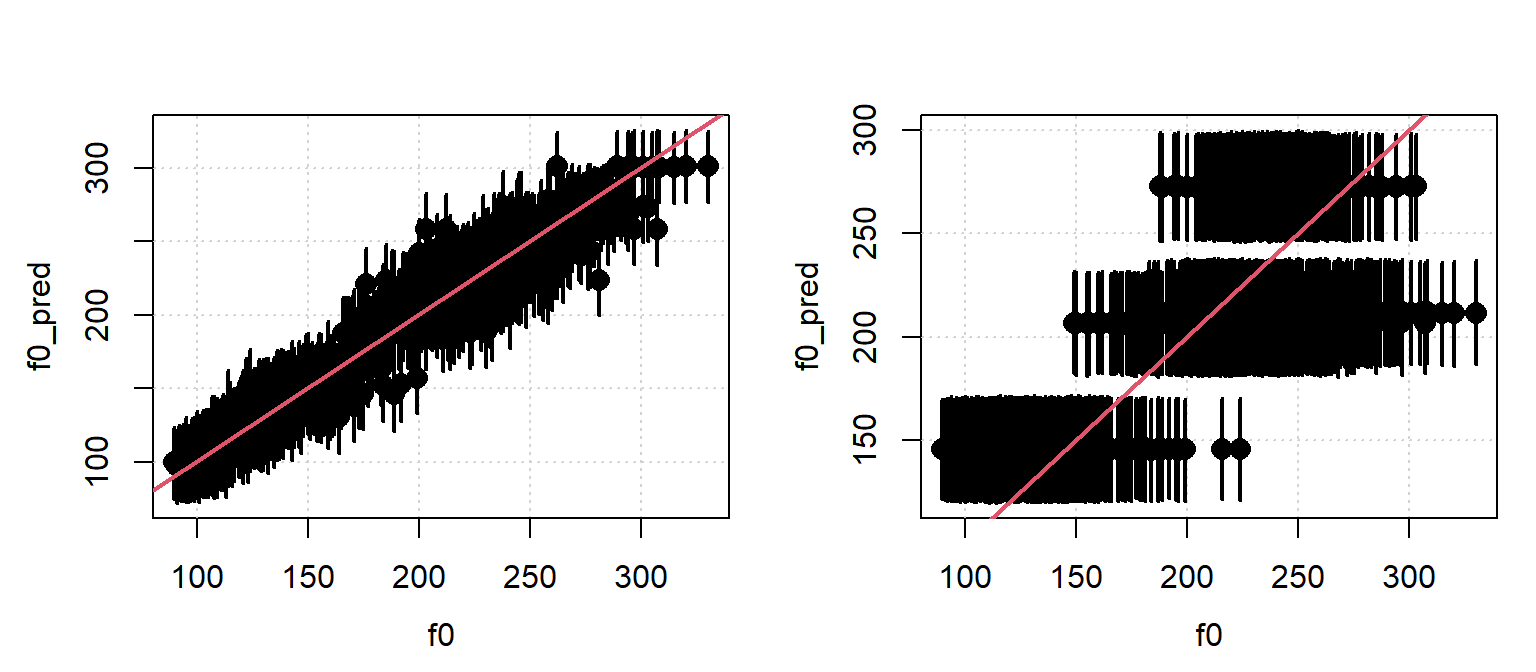
\includegraphics{04_files/figure-latex/F4-postpred1-1.pdf}
\caption{\label{fig:F4-postpred1}(left) Posterior predicted f0 for the model with speaker random effects. (right) Posterior predicted f0 for the model without speaker random effects}
\end{figure}

The above plots are good for basic analysis, but it's hard to get a good idea of the source of our problems using these plots. We can get a much better idea of how our model is performing by using an `interaction plot'.

\hypertarget{interactions-and-interaction-plots}{%
\section{Interactions and interaction plots}\label{interactions-and-interaction-plots}}

\href{http://glimo.vub.ac.be/downloads/interaction.htm}{Interactions} and understanding their graphical representations is extremely important. In many if not most models with multiple predictors, researchers will need to at least consider the effects of interactions in their models.

We can think of a single effect representing a difference between groups as a slope. For example, in the left panel below I plotted the mean f0 produced by males and female speakers from the Hillenbrand et al.~data at x-axis locations 0 and 1. The difference in the group means is -55 Hz (females 225 Hz, males 170 Hz). As a result, the line formed by joining these groups has a slope of -55 (i.e., it drops 55 Hz from 0 to 1). We can use any arbitrary x axis distance to calculate slopes, as long as we are consistent. However, there are obvious practical advantages to choosing to calculate these slopes over the arbitrary `distance' of 1. In the middle panel we see the effect for adultness, which shows a positive slope for the difference from adult to child: the f0 increases by about 60 Hz.

The plots highlighting the effects for adultness and gender are `main effects' plots. You may have heard things like ``the analysis showed a significant main effect for so and so\ldots{}''. Main effects are the average effects for one predictor averaged across everything else. Saying `averaged across everything else' basically means we are ignoring everything else. A person looking only at the left plot would not realize our data also investigates the effect of adultness. We have `erased' the differences in adultness by averaging across all levels of that factor.

Another way to think of main effects are that they are `marginal' effects. They are the overall average difference. Someone might ask you, ``whats the average difference between the f0 produced by male and female speakers in Michigan?'' and you can respond ``55 Hz''. However, sometimes the answer is not so simple, and it starts more like: ``well\ldots{} it depends''. Interactions represent situations like these, where the effect of one variable depends on, or is \emph{conditional} on, the value of some other variable.

\begin{figure}
\centering
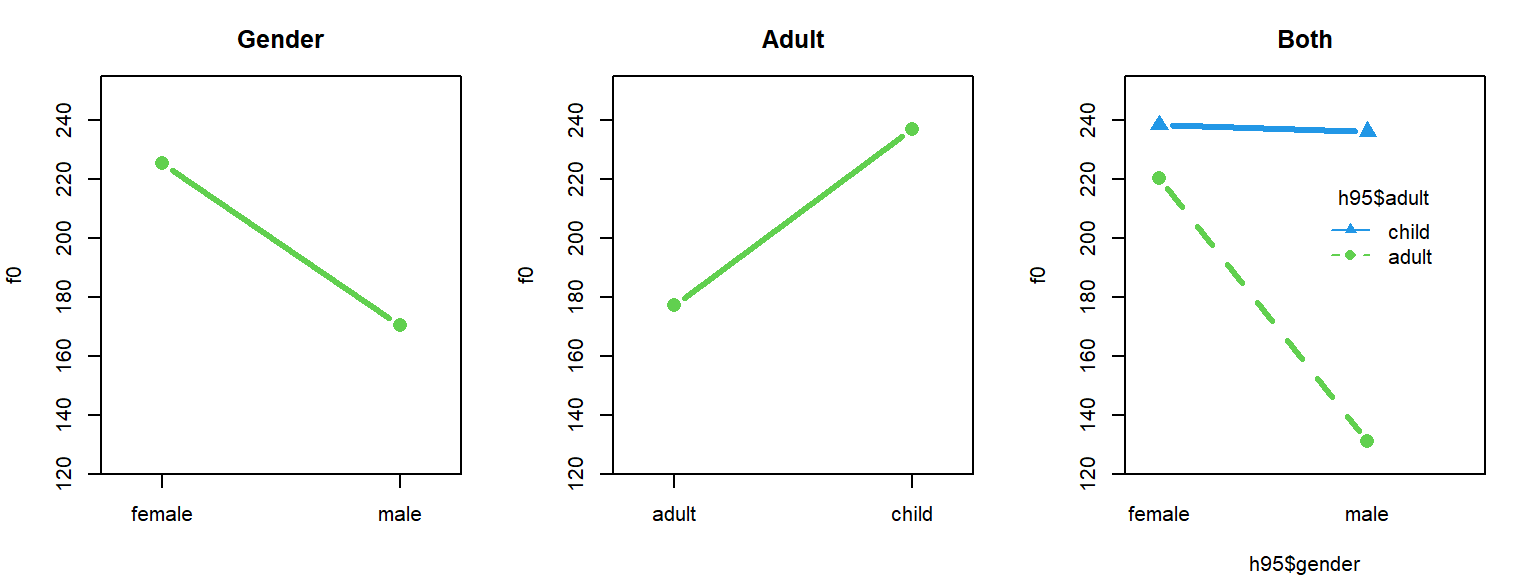
\includegraphics{04_files/figure-latex/F4-interactionplot-1.pdf}
\caption{\label{fig:F4-interactionplot}Plots showing different ways to consider our f0 data.}
\end{figure}

In the right panel above we see a two-way interaction plot. Interaction plots show you what are called the \href{http://glimo.vub.ac.be/downloads/simpleeffect.htm}{simple effects} of your predictors (sometimes also called the \emph{simple main effects}). The simple effects are the `conditional probabilities': the effects of your factor, conditional on the level of another factor. For example, the left plot shows the overall (marginal) effect for gender. The right plot also shows the effect for gender. However, it uses a blue line to show the effect for gender in adults (gender given adultness) and a green line to show the effect for children for children (gender given childness). As a result, we can consider the effects of gender \emph{conditioned} on adultness, and see how these might differ.

So, main effects show you the effect for a factor, and simple effects show you the effects of the factor \emph{depending} on the value of other things.

If adultness in no way affected f0, the right panel should look identical to the left panel. If adultness affected f0 in the same way across genders, we would see parallel lines in the right plot. This is because if you are adding a \emph{single value} to each end of the adult line, the line indicating the gender effect for adults (broken green line) would just slide up and down the f0 axis but would not change in slope. There is no way to make the green and blue lines above to match by adding a single value to either. This indicates we have an interaction in our data.

In general, when we see lines that are not parallel, that means there may be an interaction in our data. In the absence of an interaction, we could just answer the question ``whats the average difference between males and females in your sample?'' with a number like 55 Hz. In the presence of an interaction we need to consider the \emph{conditional effects} of each predictor, at the levels of the other predictor.

The idea of conditional effects \emph{feels} complicated, but it is something we all understand intuitively. How much progress will a person learning a second language make in a year? What if I told you that one group of speakers is 3 and the other is 65. You \emph{know} that makes a difference, which is to say, that you \emph{know} there is an interaction between the effect time spent learning a language, and the age at which the learner begins.

Furthermore, we all intuitively understand interactions whenever we correctly interpret the information presented in an interaction plot as above. There is a large negative slope for gender for adults. This tells us that gender has a large effect on f0 for adults. However, the slope for gender is basically zero for children. So, we might say ``there is a large f0 difference for adult males and females in our sample, but basically no gender based difference for children''. Alternatively, we might look at the changing effect for gender across adultness levels. If we did this, we might say ``there is a small effect for adultness in the average f0 produced by females, but a very large effect for adultness for males''. Anyone who is able to make such a statement based on the information in the plot above \emph{understands} interactions, whether or not they know how to relate this concept to the mathematical formalisms used to implement this concepts in regression models.

In summary, if the answer to ``what is the effect of X on Y'' is ``well, it depends on the values of Z'', you have an interaction in your data. When you have substantial interactions present in your data and you do not include these in your model, this can cause a problem for your model fit.

\hypertarget{interactions-in-our-f0-data}{%
\subsection{Interactions in our f0 data}\label{interactions-in-our-f0-data}}

Above we made posterior predictions of our data using our model, with and without the inclusion of the speaker random effects. We can see that when random effects are included, prediction is quite good. This is not surprising since the speaker-specific intercept adjustments allow for each speaker's mean f0 to be modeled effectively. However, we see that the predictions made by our model are substantially and systematically wrong in the absence of the speaker random intercepts.

It's clear that the problem with our predictions in the right panel is that the lines are parallel. As we've just discussed, in the absence of interactions, interaction plots contain only parallel lines. Well, since our model (\texttt{model\_both}) does not include interaction terms it cannot represent interactions, and so is only capable of producing predictions that result in parallel lines. This means it is not capable of representing the pattern in our data!

This is an important point worth considering. Your model is a little universe you made up, and it only includes the information you included in it. This `universe' only contains parallel lines because we only included that capability. So, the fact that your model generates parallel lines does not in any way `prove' that the lines are parallel, because they were bound to be so. In order to properly model the group differences, and to really understand whether interactions are present in the data, the model must be \emph{built} in a way that allows it to represent the interactions in our data.

\begin{Shaded}
\begin{Highlighting}[]
\FunctionTok{par}\NormalTok{ (}\AttributeTok{mfrow =} \FunctionTok{c}\NormalTok{(}\DecValTok{1}\NormalTok{,}\DecValTok{3}\NormalTok{), }\AttributeTok{mar =} \FunctionTok{c}\NormalTok{(}\DecValTok{4}\NormalTok{,}\DecValTok{4}\NormalTok{,}\DecValTok{3}\NormalTok{,}\DecValTok{2}\NormalTok{))}

\FunctionTok{plot.interaction}\NormalTok{ (h95}\SpecialCharTok{$}\NormalTok{gender, h95}\SpecialCharTok{$}\NormalTok{adult, h95}\SpecialCharTok{$}\NormalTok{f0, }\AttributeTok{col=}\DecValTok{3}\SpecialCharTok{:}\DecValTok{4}\NormalTok{, }\AttributeTok{ylim=}\FunctionTok{c}\NormalTok{(}\DecValTok{130}\NormalTok{,}\DecValTok{280}\NormalTok{),}\AttributeTok{lwd=}\DecValTok{3}\NormalTok{,}
                  \AttributeTok{type=}\StringTok{\textquotesingle{}b\textquotesingle{}}\NormalTok{,}\AttributeTok{pch=}\FunctionTok{c}\NormalTok{(}\DecValTok{16}\NormalTok{,}\DecValTok{17}\NormalTok{),}\AttributeTok{cex=}\FloatTok{1.5}\NormalTok{,}\AttributeTok{main=}\StringTok{"Data"}\NormalTok{,}\AttributeTok{legend =} \ConstantTok{FALSE}\NormalTok{)}

\FunctionTok{plot.interaction}\NormalTok{ (h95}\SpecialCharTok{$}\NormalTok{gender, h95}\SpecialCharTok{$}\NormalTok{adult, y\_pred[,}\DecValTok{1}\NormalTok{], }\AttributeTok{col =} \DecValTok{3}\SpecialCharTok{:}\DecValTok{4}\NormalTok{,}\AttributeTok{lwd=}\DecValTok{3}\NormalTok{, }\AttributeTok{type=}\StringTok{\textquotesingle{}b\textquotesingle{}}\NormalTok{,}
                  \AttributeTok{pch =} \FunctionTok{c}\NormalTok{(}\DecValTok{16}\NormalTok{,}\DecValTok{17}\NormalTok{), }\AttributeTok{cex =} \FloatTok{1.5}\NormalTok{, }\AttributeTok{ylim =} \FunctionTok{c}\NormalTok{(}\DecValTok{130}\NormalTok{,}\DecValTok{280}\NormalTok{),}
                  \AttributeTok{main=}\StringTok{"Pred. with RE"}\NormalTok{,}\AttributeTok{legend=}\ConstantTok{FALSE}\NormalTok{)}

\FunctionTok{plot.interaction}\NormalTok{ (h95}\SpecialCharTok{$}\NormalTok{gender, h95}\SpecialCharTok{$}\NormalTok{adult, y\_pred\_no\_re[,}\DecValTok{1}\NormalTok{],}\AttributeTok{col=}\DecValTok{3}\SpecialCharTok{:}\DecValTok{4}\NormalTok{, }\AttributeTok{lwd=}\DecValTok{3}\NormalTok{,}
                  \AttributeTok{type =} \StringTok{\textquotesingle{}b\textquotesingle{}}\NormalTok{, }\AttributeTok{pch =} \FunctionTok{c}\NormalTok{(}\DecValTok{16}\NormalTok{,}\DecValTok{17}\NormalTok{), }\AttributeTok{cex =} \FloatTok{1.5}\NormalTok{, }\AttributeTok{ylim =} \FunctionTok{c}\NormalTok{(}\DecValTok{130}\NormalTok{,}\DecValTok{280}\NormalTok{),}
                  \AttributeTok{main=}\StringTok{"Pred. without RE"}\NormalTok{, }\AttributeTok{leg.x=}\FloatTok{1.8}\NormalTok{,}\AttributeTok{leg.y=}\DecValTok{270}\NormalTok{, }\AttributeTok{xlim=}\FunctionTok{c}\NormalTok{(.}\DecValTok{95}\NormalTok{,}\FloatTok{2.3}\NormalTok{))}
\end{Highlighting}
\end{Shaded}

\begin{figure}
\centering
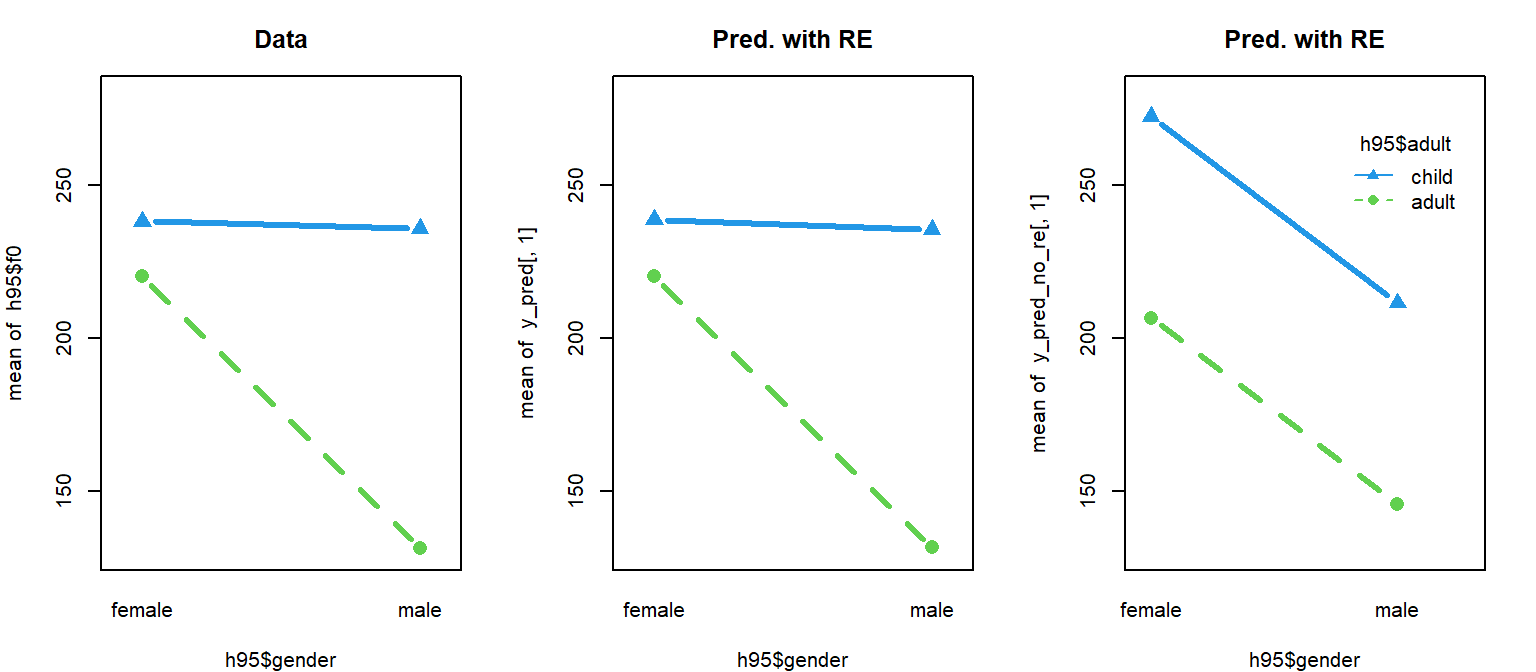
\includegraphics{04_files/figure-latex/interactionplot3-1.pdf}
\caption{\label{fig:interactionplot3}Interaction plots showing comparing our f0 data to different posterior predictions, with and without RE (random effects).}
\end{figure}

\hypertarget{investigating-interactions-with-a-model}{%
\section{Investigating interactions with a model}\label{investigating-interactions-with-a-model}}

The model presented above (\texttt{model\_both}) requires only a slight tweak to include a term representing the interaction in our data. There are two ways to include interactions in R model formulas, as shown below:

\texttt{f0\ \textasciitilde{}\ adult\ +\ gender\ +\ adult:gender\ +\ (1\textbar{}speaker)}
~

\texttt{f0\ \textasciitilde{}\ adult\ *\ gender\ +\ (1\textbar{}speaker)}

The first way includes an explicit interaction term, \texttt{adult:gender}. The syntax for these is \texttt{X:Z} for an interaction between effects \texttt{X} and \texttt{Z}, \texttt{W:X:Z} for a three-way interaction, and so on. The second way uses \texttt{*} between our two predictors. This tells R to include those predictors, and the interactions between them This can be much faster then specifying all interactions, but you lose control over which ones you include. For example the first formula implies the second, but cannot represent the third (since it omits one interaction):

\texttt{y\ \textasciitilde{}\ Z\ *\ X\ *\ W}
~

\texttt{y\ \textasciitilde{}\ Z\ +\ X\ +\ W\ +\ Z:X\ +\ Z:W\ +\ X:W\ +\ Z:X:W}
~

\texttt{y\ \textasciitilde{}\ Z\ +\ X\ +\ W\ +\ Z:X\ +\ X:W\ +\ Z:X:W}

Our full model specification now includes an \emph{interaction} term that can help explain variation that cannot be explained by the independent effects of adultness and gender. This interaction term helps us model the \emph{conditional} effect of one predictor given the other.

\begin{equation}
\begin{split}
\textrm{Likelihood:} \\
y_{[i]} \sim \mathcal{N}(\mu_{[i]},\sigma_{error}) \\
\mu_{[i]} = Intercept + adult_{\textrm{adult}_{[i]}} + gender_{\textrm{gender}_{[i]}}+ adult:gender + \alpha_{speaker_{[i]}} \\\\
\textrm{Priors:} \\
\alpha_{speaker} \sim \mathcal{N}(0,\sigma_{speaker}) \\ \\ 
Intercept \sim t(3, 200, 100) \\ 
adult_{[i]} \sim t(3, 0, 100) \\ 
gender_{[i]} \sim t(3, 0, 100) \\ 
adult:gender \sim t(3, 0, 100) \\ 
\sigma_{error} \sim t(3, 0, 100) \\
\sigma_{speaker} \sim t(3, 0, 100) \\ 
\end{split}
\label{eq:43}
\end{equation}

\hypertarget{fitting-the-model-and-interpreting-the-results-1}{%
\subsection{Fitting the model and interpreting the results}\label{fitting-the-model-and-interpreting-the-results-1}}

Below I fit the model which now includes an interaction term representing the changing effect of gender and adultness on average f0.

\begin{Shaded}
\begin{Highlighting}[]
\CommentTok{\# Fit the model yourself, or download pre{-}fit model from: }
\CommentTok{\# github.com/santiagobarreda/stats{-}class/tree/master/models}
\CommentTok{\# and load after placing in working directory}
\CommentTok{\#  model\_interaction = readRDS (\textquotesingle{}4\_model\_interaction.RDS\textquotesingle{})}

\FunctionTok{set.seed}\NormalTok{ (}\DecValTok{1}\NormalTok{)}
\NormalTok{model\_interaction }\OtherTok{=}  
  \FunctionTok{brm}\NormalTok{ (f0 }\SpecialCharTok{\textasciitilde{}}\NormalTok{ adult }\SpecialCharTok{+}\NormalTok{ gender }\SpecialCharTok{+}\NormalTok{ adult}\SpecialCharTok{:}\NormalTok{gender }\SpecialCharTok{+}\NormalTok{ (}\DecValTok{1}\SpecialCharTok{|}\NormalTok{speaker), }\AttributeTok{data =}\NormalTok{ h95, }
       \AttributeTok{chains =} \DecValTok{4}\NormalTok{, }\AttributeTok{cores =} \DecValTok{4}\NormalTok{, }\AttributeTok{warmup =} \DecValTok{1000}\NormalTok{, }\AttributeTok{iter =} \DecValTok{11000}\NormalTok{, }\AttributeTok{thin =} \DecValTok{10}\NormalTok{, }
       \AttributeTok{prior =} \FunctionTok{c}\NormalTok{(}\FunctionTok{set\_prior}\NormalTok{(}\StringTok{"student\_t(3, 200, 100)"}\NormalTok{, }\AttributeTok{class =} \StringTok{"Intercept"}\NormalTok{),}
                              \FunctionTok{set\_prior}\NormalTok{(}\StringTok{"student\_t(3, 0, 100)"}\NormalTok{, }\AttributeTok{class =} \StringTok{"b"}\NormalTok{),}
                              \FunctionTok{set\_prior}\NormalTok{(}\StringTok{"student\_t(3, 0, 100)"}\NormalTok{, }\AttributeTok{class =} \StringTok{"sd"}\NormalTok{))) }

\CommentTok{\#  saveRDS (model\_interaction, \textquotesingle{}4\_model\_interaction.RDS\textquotesingle{})}
\end{Highlighting}
\end{Shaded}

\begin{Shaded}
\begin{Highlighting}[]
\CommentTok{\# inspect model}
\NormalTok{model\_interaction}
\end{Highlighting}
\end{Shaded}

\begin{verbatim}
##  Family: gaussian 
##   Links: mu = identity; sigma = identity 
## Formula: f0 ~ adult + gender + adult:gender + (1 | speaker) 
##    Data: h95 (Number of observations: 1668) 
## Samples: 4 chains, each with iter = 11000; warmup = 1000; thin = 10;
##          total post-warmup samples = 4000
## 
## Group-Level Effects: 
## ~speaker (Number of levels: 139) 
##               Estimate Est.Error l-95% CI u-95% CI Rhat Bulk_ESS Tail_ESS
## sd(Intercept)    20.92      1.33    18.52    23.77 1.00     3027     3703
## 
## Population-Level Effects: 
##                Estimate Est.Error l-95% CI u-95% CI Rhat Bulk_ESS Tail_ESS
## Intercept        206.56      1.91   202.78   210.27 1.00     2418     3405
## adult1           -30.67      1.94   -34.47   -26.88 1.00     1911     2938
## gender1           22.89      1.97    18.94    26.76 1.00     1851     3038
## adult1:gender1    21.72      1.92    17.87    25.46 1.00     2242     3328
## 
## Family Specific Parameters: 
##       Estimate Est.Error l-95% CI u-95% CI Rhat Bulk_ESS Tail_ESS
## sigma    11.86      0.21    11.46    12.29 1.00     4012     4098
## 
## Samples were drawn using sampling(NUTS). For each parameter, Bulk_ESS
## and Tail_ESS are effective sample size measures, and Rhat is the potential
## scale reduction factor on split chains (at convergence, Rhat = 1).
\end{verbatim}

Remember that this line \texttt{set\_prior("student\_t(3,\ 0,\ 100)",\ class\ =\ "b")} sets the prior for all non-intercept `Population-Level' predictors. This allows you to efficiently set priors for the adult, gender, and adult:gender predictors in your model in a single line, and becomes more and more useful as our models grow more complex.

A look at the model output above indicates that we have a large interaction term. In fact, our interaction is as large as the `main' effect for gender! In cases with large interactions we have to be very careful about interpreting the main effects. In other words, when the answer to a question is ``it really depends'', you should be wary of making blanket statements.

We need to talk about why there is only a single interaction term. The reason for this is related to the same reason we can't get estimates for all our group effects (i.e., linear dependence). The number of terms you can estimate is generally one fewer than the number of levels. For interaction terms, the number of parameters is equal to (number of levels of factor (A - 1)x(number of levels of factor B - 1). Since each of our factors have two levels, we can only estimate one parameter, (2-1)x(2-1).

Our interaction basically says that sometimes being a male \emph{and} being an adult results in a lower f0 than can be predicted independently by maleness and adultness. So, you only need one coefficient to represent the extra combined effects of maleness \emph{and} adultness. This same coefficient can also represent the opposite case: not male and not adult. You don't need an interaction term to model the effect of maleness \emph{or} adultness since that is effectively what the main effects do (i.e., model the effect regardless of the difference of the other value).

The interaction term is just another element of your prediction equation (i.e., \(\mu + x_1+x_2...\)) intended to help explain variation that can't be predicted by the independent effects of the other predictors in the model. Recovering the predicted group means based on the coefficient values is straightforward, but a bit tedious: we must now either add or subtract the value of the interaction term (\texttt{adult1:gender1}) from each group. We can easily determine which to do for this model because the sign on the interaction term is the product of the signs on the relevant `main effects' terms.

For example, the second hypothesis we are testing below says \texttt{Intercept\ +\ -adult1\ +\ -gender1\ +\ adult1:gender1\ =\ 0}. This could be read like ``take the overall mean, add the effect for `child' (or \texttt{adult2}, since \texttt{-adult1=adult2}), and add the effect for `male' (or \texttt{gender2} since \texttt{-gender1=gender2}), and add the effect for when the speaker is male \emph{and} a child (\texttt{-adult1*-gender1\ =\ +adult1:gender1})''. If you look at the hypotheses below, you will see that the sign on the interaction terms solely depends on the signs of the corresponding main effects terms. We can see that the inclusion of an interaction term allows our model to capture group averages more accurately than the model without intercepts.

\begin{Shaded}
\begin{Highlighting}[]
\CommentTok{\# actual data means}
\FunctionTok{tapply}\NormalTok{ (h95}\SpecialCharTok{$}\NormalTok{f0, h95}\SpecialCharTok{$}\NormalTok{group, mean)}
\DocumentationTok{\#\#        b        g        m        w }
\DocumentationTok{\#\# 236.0741 238.3509 131.2185 220.4010}
\CommentTok{\# intercept, boys, girls, men, women}
\NormalTok{means\_pred\_interaction }\OtherTok{=}\NormalTok{ brms}\SpecialCharTok{::}\FunctionTok{hypothesis}\NormalTok{ (model\_interaction, }
              \FunctionTok{c}\NormalTok{(}\StringTok{"Intercept = 0"}\NormalTok{,}
                \StringTok{"Intercept + {-}adult1 + {-}gender1 +  adult1:gender1 = 0"}\NormalTok{,}
                \StringTok{"Intercept + {-}adult1 +  gender1 + {-}adult1:gender1 = 0"}\NormalTok{,}
                \StringTok{"Intercept +  adult1 + {-}gender1 + {-}adult1:gender1 = 0"}\NormalTok{,}
                \StringTok{"Intercept +  adult1 +  gender1 +  adult1:gender1 = 0"}\NormalTok{))[[}\DecValTok{1}\NormalTok{]][,}\DecValTok{1}\SpecialCharTok{:}\DecValTok{5}\NormalTok{]}
\CommentTok{\# predictions with no interaction term}
\NormalTok{means\_pred}
\DocumentationTok{\#\#                         Hypothesis Estimate Est.Error CI.Lower CI.Upper}
\DocumentationTok{\#\# 1                  (Intercept) = 0 209.1341  2.660729 203.9475 214.3788}
\DocumentationTok{\#\# 2 (Intercept+{-}adult1+{-}gender1) = 0 211.5892  4.840349 202.1583 221.4233}
\DocumentationTok{\#\# 3  (Intercept+{-}adult1+gender1) = 0 272.5741  5.390701 262.0859 283.0745}
\DocumentationTok{\#\# 4  (Intercept+adult1+{-}gender1) = 0 145.6940  4.010808 137.7944 153.4169}
\DocumentationTok{\#\# 5   (Intercept+adult1+gender1) = 0 206.6789  3.814463 199.1961 214.2051}

\CommentTok{\# predictions with interaction term}
\NormalTok{means\_pred\_interaction}
\DocumentationTok{\#\#                                        Hypothesis Estimate Est.Error CI.Lower}
\DocumentationTok{\#\# 1                                 (Intercept) = 0 206.5611  1.913081 202.7834}
\DocumentationTok{\#\# 2 (Intercept+{-}adult1+{-}gender1+adult1:gender1) = 0 236.0571  4.190763 227.9085}
\DocumentationTok{\#\# 3 (Intercept+{-}adult1+gender1+{-}adult1:gender1) = 0 238.4038  4.809069 229.0110}
\DocumentationTok{\#\# 4 (Intercept+adult1+{-}gender1+{-}adult1:gender1) = 0 131.2809  3.184129 124.9046}
\DocumentationTok{\#\# 5   (Intercept+adult1+gender1+adult1:gender1) = 0 220.5027  3.021626 214.4826}
\DocumentationTok{\#\#   CI.Upper}
\DocumentationTok{\#\# 1 210.2747}
\DocumentationTok{\#\# 2 244.4526}
\DocumentationTok{\#\# 3 247.6442}
\DocumentationTok{\#\# 4 137.3878}
\DocumentationTok{\#\# 5 226.4404}
\end{Highlighting}
\end{Shaded}

Below I print the estimates of the `fixed' effects in the model so we can focus on those. If you fit a model like this and are having trouble interpreting it, I would really encourage you to write down an interpretation using pen and paper, focusing on the decomposition of values provided by the regression model.

\begin{Shaded}
\begin{Highlighting}[]
\NormalTok{brms}\SpecialCharTok{::}\FunctionTok{fixef}\NormalTok{ (model\_interaction)}
\DocumentationTok{\#\#                 Estimate Est.Error      Q2.5     Q97.5}
\DocumentationTok{\#\# Intercept      206.56112  1.913081 202.78344 210.27475}
\DocumentationTok{\#\# adult1         {-}30.66934  1.936608 {-}34.46529 {-}26.87641}
\DocumentationTok{\#\# gender1         22.89211  1.974245  18.93775  26.76101}
\DocumentationTok{\#\# adult1:gender1  21.71878  1.918765  17.86664  25.46130}
\end{Highlighting}
\end{Shaded}

For example, the average f0 is 206. The gender difference is 44 Hz (22 * 2) between groups, and there is a gender-based 23 Hz deviation from the mean between groups. This means that, overall, the male and female averages are about 183 and 229 Hz (206 ± 22).

However, the \texttt{adult1:gender1} interaction is 22 Hz. This means that when the speaker was an adult (\texttt{adult1}), the gender difference was nearly doubled. We know this because the effect for \texttt{gender1} is 22.8, and the effect for \texttt{gender1} \textbf{given} \texttt{adult1} (\texttt{adult1:gender1}, which is the same thing as \texttt{gender1:adult1}) is 21.7 Hz higher than that. So, the total effect for f0 across adults is about 22.8 + 21.7 = 44.5, suggesting a difference in f0 between the groups of 89 Hz (44.5 * 2).

I am going to basically restate what I just said because it is very important. The effect for \texttt{gender} is 22.8, and the effect for \texttt{gender1:adult1} is further 21.7 Hz. As a result, the cumulative effect for gender1 (female) given adult1 (adult) is \texttt{gender1\ +\ gender1:adult1\ =\ 44.5}.

In contrast, the fact that \texttt{adult1:gender1\ =\ 21.7} indicates that \texttt{adult2:gender1\ =\ -21.7}. This is because since \texttt{adult1:gender1} represents the effect of \texttt{gender1} \emph{given} \texttt{adult1}, the effect given \texttt{adult2} must be opposite in sign (because of sum coding). So, we can say that although the effect for gender is 22.9 overall, given that the speaker is a child (\texttt{adult2}), this effect is 21.7 Hz lower than the `main effect' estimate. So, for children we expect an f0 effect of 22.9 - 21.7 = 1.2, suggesting a group difference of 2.2 Hz. In other words, the effect of gender is basically zero given that the speakers are children.

We can consider the effects the other way. The marginal effect for \texttt{adult1} is -30, meaning that when speakers are adults, their f0 is 30 Hz lower than the overall average. However, \texttt{adult1:gender1\ =\ 21.7}, meaning that \emph{if} the speaker is female (\texttt{gender1}), then the expected effect of adultness is reduced (-30 + 21.7 = -8.3) so that the expected group difference is only 17 Hz. On the other hand, when the speaker is a male (\texttt{gender2}) then the interaction term should be flipped in sign (\texttt{adult1:gender2\ =\ \ -21.7}). This means that the effect of adultness, conditional on the speaker being male is nearly doubled (-30 + -21.7 = -51.7).

When considered in this way all these coefficients are just telling us what we already knew from looking at the interaction plot: f0 varies substantially based on gender for adults but not for children. Or: f0 varies substantially as a function of adultness for males but much less for females.

\hypertarget{assessing-model-fit}{%
\subsection{Assessing model fit}\label{assessing-model-fit}}

We can asses model fit for the model including interaction terms by making more posterior predictions with our new model.

\begin{Shaded}
\begin{Highlighting}[]
\NormalTok{y\_pred\_int }\OtherTok{=} \FunctionTok{predict}\NormalTok{ (model\_interaction)}
\NormalTok{y\_pred\_no\_re\_int }\OtherTok{=} \FunctionTok{predict}\NormalTok{ (model\_interaction, }\AttributeTok{re\_formula =} \ConstantTok{NA}\NormalTok{)}
\end{Highlighting}
\end{Shaded}

We can make more interaction plots using our data and our posterior predictions. Below I compare our data, the predictions of our original model, and the predictions of our model that includes interactions. Whereas the model with no interactions enforced parallelism on the effects, our new model is able to capture the conditional nature of gender given adultness in our data.

\begin{Shaded}
\begin{Highlighting}[]
\FunctionTok{par}\NormalTok{ (}\AttributeTok{mfrow =} \FunctionTok{c}\NormalTok{(}\DecValTok{1}\NormalTok{,}\DecValTok{3}\NormalTok{), }\AttributeTok{mar =} \FunctionTok{c}\NormalTok{(}\DecValTok{4}\NormalTok{,}\DecValTok{4}\NormalTok{,}\DecValTok{3}\NormalTok{,}\DecValTok{2}\NormalTok{))}

\FunctionTok{plot.interaction}\NormalTok{ (h95}\SpecialCharTok{$}\NormalTok{gender, h95}\SpecialCharTok{$}\NormalTok{adult, h95}\SpecialCharTok{$}\NormalTok{f0, }\AttributeTok{col=}\DecValTok{3}\SpecialCharTok{:}\DecValTok{4}\NormalTok{, }\AttributeTok{ylim=}\FunctionTok{c}\NormalTok{(}\DecValTok{130}\NormalTok{,}\DecValTok{280}\NormalTok{),}\AttributeTok{lwd=}\DecValTok{3}\NormalTok{,}
                  \AttributeTok{type=}\StringTok{\textquotesingle{}b\textquotesingle{}}\NormalTok{,}\AttributeTok{pch=}\FunctionTok{c}\NormalTok{(}\DecValTok{16}\NormalTok{,}\DecValTok{17}\NormalTok{),}\AttributeTok{cex=}\FloatTok{1.5}\NormalTok{,}\AttributeTok{main=}\StringTok{"Data"}\NormalTok{,}\AttributeTok{legend =} \ConstantTok{FALSE}\NormalTok{)}

\FunctionTok{plot.interaction}\NormalTok{ (h95}\SpecialCharTok{$}\NormalTok{gender, h95}\SpecialCharTok{$}\NormalTok{adult, y\_pred\_no\_re[,}\DecValTok{1}\NormalTok{],}\AttributeTok{col=}\DecValTok{3}\SpecialCharTok{:}\DecValTok{4}\NormalTok{, }\AttributeTok{lwd=}\DecValTok{3}\NormalTok{,}
                  \AttributeTok{type =} \StringTok{\textquotesingle{}b\textquotesingle{}}\NormalTok{, }\AttributeTok{pch =} \FunctionTok{c}\NormalTok{(}\DecValTok{16}\NormalTok{,}\DecValTok{17}\NormalTok{), }\AttributeTok{cex =} \FloatTok{1.5}\NormalTok{, }\AttributeTok{ylim =} \FunctionTok{c}\NormalTok{(}\DecValTok{130}\NormalTok{,}\DecValTok{280}\NormalTok{),}
                  \AttributeTok{main=}\StringTok{"No Int. no RE"}\NormalTok{, }\AttributeTok{legend =} \ConstantTok{FALSE}\NormalTok{)}

\FunctionTok{plot.interaction}\NormalTok{ (h95}\SpecialCharTok{$}\NormalTok{gender, h95}\SpecialCharTok{$}\NormalTok{adult, y\_pred\_no\_re\_int[,}\DecValTok{1}\NormalTok{],}\AttributeTok{col=}\DecValTok{3}\SpecialCharTok{:}\DecValTok{4}\NormalTok{, }\AttributeTok{lwd=}\DecValTok{3}\NormalTok{,}
                  \AttributeTok{type =} \StringTok{\textquotesingle{}b\textquotesingle{}}\NormalTok{, }\AttributeTok{pch =} \FunctionTok{c}\NormalTok{(}\DecValTok{16}\NormalTok{,}\DecValTok{17}\NormalTok{), }\AttributeTok{cex =} \FloatTok{1.5}\NormalTok{, }\AttributeTok{ylim =} \FunctionTok{c}\NormalTok{(}\DecValTok{130}\NormalTok{,}\DecValTok{280}\NormalTok{),}
                  \AttributeTok{main=}\StringTok{"With Int. no RE"}\NormalTok{, }\AttributeTok{leg.x=}\FloatTok{1.8}\NormalTok{,}\AttributeTok{leg.y=}\DecValTok{270}\NormalTok{, }\AttributeTok{xlim=}\FunctionTok{c}\NormalTok{(.}\DecValTok{95}\NormalTok{,}\FloatTok{2.3}\NormalTok{))}
\end{Highlighting}
\end{Shaded}

\begin{figure}
\centering
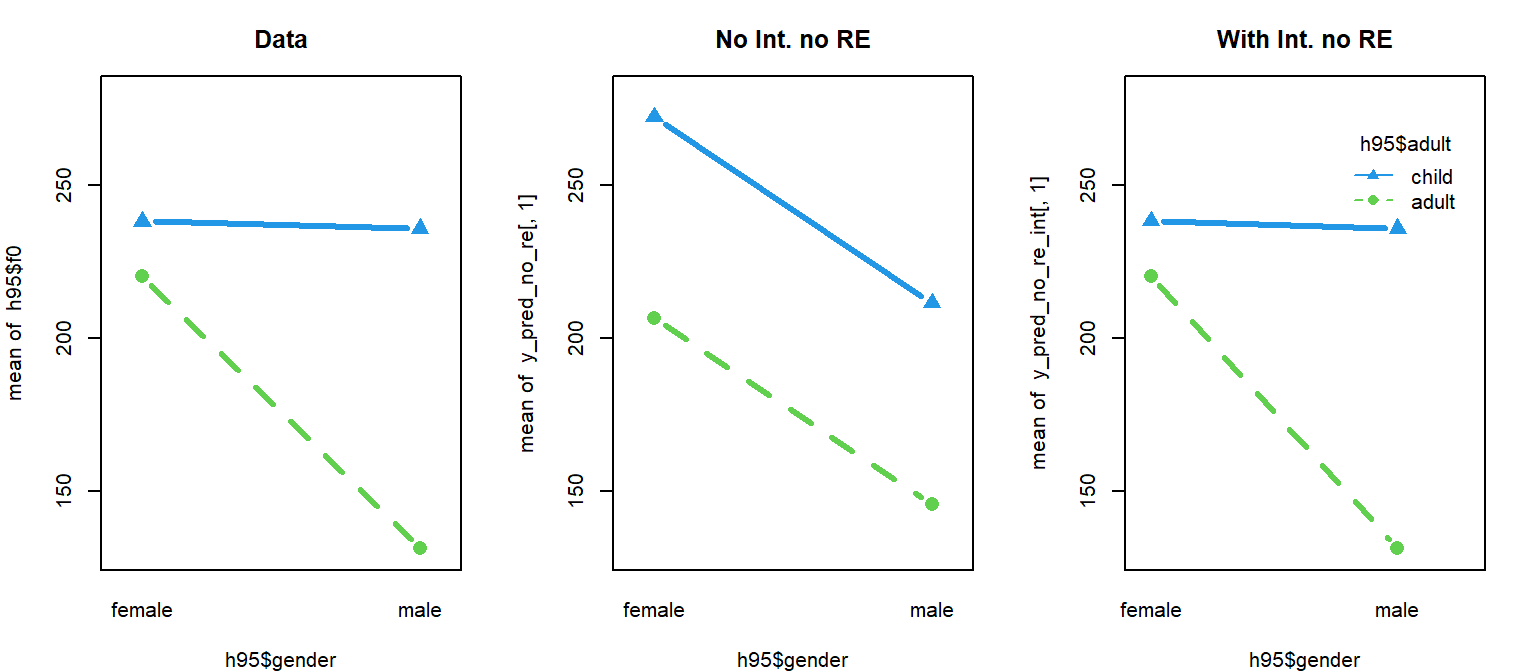
\includegraphics{04_files/figure-latex/interactionplot2-1.pdf}
\caption{\label{fig:interactionplot2}Interaction plots showing comparing our f0 data to posterior predictions, with and without interaction terms (neither contains Random Effects).}
\end{figure}

For the first time, we have a model that really does a reasonably-good job of representing the information in our data. The model can capture the gender-dependent nature of age-based f0 differences, and separately estimates between group variation and between group variation.

\hypertarget{investigating-the-interactions-the-easy-way}{%
\subsection{Investigating the interactions the easy way}\label{investigating-the-interactions-the-easy-way}}

There are built-in functions in \texttt{brms} that help you investigate your effects in the presence of interactions. The \texttt{conditional\_effects} function calculates the values of effects conditional on the Intercept (for continuous variables). This means it adds the value of the Intercept to all its effects estimates. This function is extremely handy but also limited. You can't get the posterior samples from this function, meaning you can't use this output to compare the values of rows. Also, conditioning on the mean introduces noise to our effects estimates and makes their credible intervals larger.

\begin{Shaded}
\begin{Highlighting}[]
\CommentTok{\# group means}
\FunctionTok{tapply}\NormalTok{ (h95}\SpecialCharTok{$}\NormalTok{f0, h95}\SpecialCharTok{$}\NormalTok{group, mean)}
\DocumentationTok{\#\#        b        g        m        w }
\DocumentationTok{\#\# 236.0741 238.3509 131.2185 220.4010}

\CommentTok{\# get conditional effects}
\NormalTok{model\_effects }\OtherTok{=} \FunctionTok{conditional\_effects}\NormalTok{ (model\_interaction)}

\CommentTok{\# adultness effect (average for adult vs children)}
\NormalTok{model\_effects[[}\DecValTok{1}\NormalTok{]][,}\SpecialCharTok{{-}}\FunctionTok{c}\NormalTok{(}\DecValTok{1}\SpecialCharTok{:}\DecValTok{5}\NormalTok{)]}
\DocumentationTok{\#\#   effect1\_\_ estimate\_\_     se\_\_  lower\_\_  upper\_\_}
\DocumentationTok{\#\# 1     adult   220.5119 2.950740 214.4826 226.4404}
\DocumentationTok{\#\# 2     child   238.4238 4.839866 229.0110 247.6442}

\CommentTok{\# gender effect (average for females vs males)}
\NormalTok{model\_effects[[}\DecValTok{2}\NormalTok{]][,}\SpecialCharTok{{-}}\FunctionTok{c}\NormalTok{(}\DecValTok{1}\SpecialCharTok{:}\DecValTok{5}\NormalTok{)]}
\DocumentationTok{\#\#   effect1\_\_ estimate\_\_     se\_\_  lower\_\_  upper\_\_}
\DocumentationTok{\#\# 1    female   220.5119 2.950740 214.4826 226.4404}
\DocumentationTok{\#\# 2      male   131.3351 3.191314 124.9046 137.3878}

\CommentTok{\# recreated group means for w, m, g, b}
\NormalTok{model\_effects[[}\DecValTok{3}\NormalTok{]][,}\SpecialCharTok{{-}}\FunctionTok{c}\NormalTok{(}\DecValTok{1}\SpecialCharTok{:}\DecValTok{5}\NormalTok{)]}
\DocumentationTok{\#\#   effect1\_\_ effect2\_\_ estimate\_\_     se\_\_  lower\_\_  upper\_\_}
\DocumentationTok{\#\# 1     adult    female   220.5119 2.950740 214.4826 226.4404}
\DocumentationTok{\#\# 2     adult      male   131.3351 3.191314 124.9046 137.3878}
\DocumentationTok{\#\# 3     child    female   238.4238 4.839866 229.0110 247.6442}
\DocumentationTok{\#\# 4     child      male   236.0509 4.175498 227.9085 244.4526}
\end{Highlighting}
\end{Shaded}

The \texttt{marginal\_effects} function returns a list of matrices. Each one contains a different main effect or interaction term. Above I print each one in turn. We can see that these values match those we recreated above using the\texttt{hypothesis} function and the individual coefficients:

\begin{Shaded}
\begin{Highlighting}[]
\FunctionTok{tapply}\NormalTok{ (h95}\SpecialCharTok{$}\NormalTok{f0, h95}\SpecialCharTok{$}\NormalTok{group, mean)}
\DocumentationTok{\#\#        b        g        m        w }
\DocumentationTok{\#\# 236.0741 238.3509 131.2185 220.4010}
\NormalTok{brms}\SpecialCharTok{::}\FunctionTok{hypothesis}\NormalTok{ (model\_interaction, }\FunctionTok{c}\NormalTok{(}
                \StringTok{"Intercept = 0"}\NormalTok{,}
                \StringTok{"Intercept + {-}adult1 + {-}gender1 +  adult1:gender1 = 0"}\NormalTok{,}
                \StringTok{"Intercept + {-}adult1 +  gender1 + {-}adult1:gender1 = 0"}\NormalTok{,}
                \StringTok{"Intercept +  adult1 + {-}gender1 + {-}adult1:gender1 = 0"}\NormalTok{,}
                \StringTok{"Intercept +  adult1 +  gender1 +  adult1:gender1 = 0"}\NormalTok{))[[}\DecValTok{1}\NormalTok{]][,}\DecValTok{2}\SpecialCharTok{:}\DecValTok{5}\NormalTok{]}
\DocumentationTok{\#\#   Estimate Est.Error CI.Lower CI.Upper}
\DocumentationTok{\#\# 1 206.5611  1.913081 202.7834 210.2747}
\DocumentationTok{\#\# 2 236.0571  4.190763 227.9085 244.4526}
\DocumentationTok{\#\# 3 238.4038  4.809069 229.0110 247.6442}
\DocumentationTok{\#\# 4 131.2809  3.184129 124.9046 137.3878}
\DocumentationTok{\#\# 5 220.5027  3.021626 214.4826 226.4404}
\end{Highlighting}
\end{Shaded}

\hypertarget{making-plots}{%
\subsection{Making plots}\label{making-plots}}

There are many ways to make `nice' graphics using brms models. Many use packages like \texttt{ggplot2} and \texttt{bayesplot}. In general these figures are nice but sometimes too `fancy' for many purposes where simple black and white graphics are needed. I also don't really know how to use \texttt{ggplot2} ( :\textbar{} ). As a result, I'm going to focus on making simple line plots (like those common in journal articles) using base R graphics.

The standard information provided in the output of \texttt{brm} model summaries can be used to make plots. These summaries always contain (among other things) these four columns in the same order: the mean estimate, the standard deviation, and the lower and upper credible intervals. I wrote a small function called \texttt{brmplot} that will help draw effects plots easily using these summaries. The \texttt{brmplot} function takes in a matrix containing these columns and makes plots showing the means and credible intervals of different effects, assuming that each row is an effect.

Below I get a summary of the fixed effects. I make plots of these effects in two orientations. In each one I omit the Intercept estimate as the magnitude of this is so different that it cannot easily be included on the plot. There is nothing special about these plots, but they are extremely effective at quickly communicating model information.

\begin{Shaded}
\begin{Highlighting}[]
\NormalTok{fixef\_interaction }\OtherTok{=}\NormalTok{ brms}\SpecialCharTok{::}\FunctionTok{fixef}\NormalTok{ (model\_interaction)}

\NormalTok{fixef\_interaction}
\DocumentationTok{\#\#                 Estimate Est.Error      Q2.5     Q97.5}
\DocumentationTok{\#\# Intercept      206.56112  1.913081 202.78344 210.27475}
\DocumentationTok{\#\# adult1         {-}30.66934  1.936608 {-}34.46529 {-}26.87641}
\DocumentationTok{\#\# gender1         22.89211  1.974245  18.93775  26.76101}
\DocumentationTok{\#\# adult1:gender1  21.71878  1.918765  17.86664  25.46130}
\end{Highlighting}
\end{Shaded}

\begin{Shaded}
\begin{Highlighting}[]
\FunctionTok{par}\NormalTok{ (}\AttributeTok{mfrow =}\FunctionTok{c}\NormalTok{(}\DecValTok{1}\NormalTok{,}\DecValTok{2}\NormalTok{), }\AttributeTok{mar =} \FunctionTok{c}\NormalTok{(}\DecValTok{8}\NormalTok{,}\DecValTok{3}\NormalTok{,}\DecValTok{1}\NormalTok{,}\DecValTok{1}\NormalTok{))}
\FunctionTok{brmplot}\NormalTok{ (fixef\_interaction[}\SpecialCharTok{{-}}\DecValTok{1}\NormalTok{,]) ; }\FunctionTok{abline}\NormalTok{ (}\AttributeTok{h =} \DecValTok{0}\NormalTok{,}\AttributeTok{lty=}\DecValTok{3}\NormalTok{)}
\FunctionTok{par}\NormalTok{ (}\AttributeTok{mar =} \FunctionTok{c}\NormalTok{(}\DecValTok{3}\NormalTok{,}\DecValTok{8}\NormalTok{,}\DecValTok{1}\NormalTok{,}\DecValTok{1}\NormalTok{))}
\FunctionTok{brmplot}\NormalTok{ (fixef\_interaction[}\SpecialCharTok{{-}}\DecValTok{1}\NormalTok{,], }\AttributeTok{horizontal =} \ConstantTok{FALSE}\NormalTok{) ; }\FunctionTok{abline}\NormalTok{ (}\AttributeTok{v=}\DecValTok{0}\NormalTok{,}\AttributeTok{lty=}\DecValTok{3}\NormalTok{)}
\end{Highlighting}
\end{Shaded}

\begin{figure}
\centering
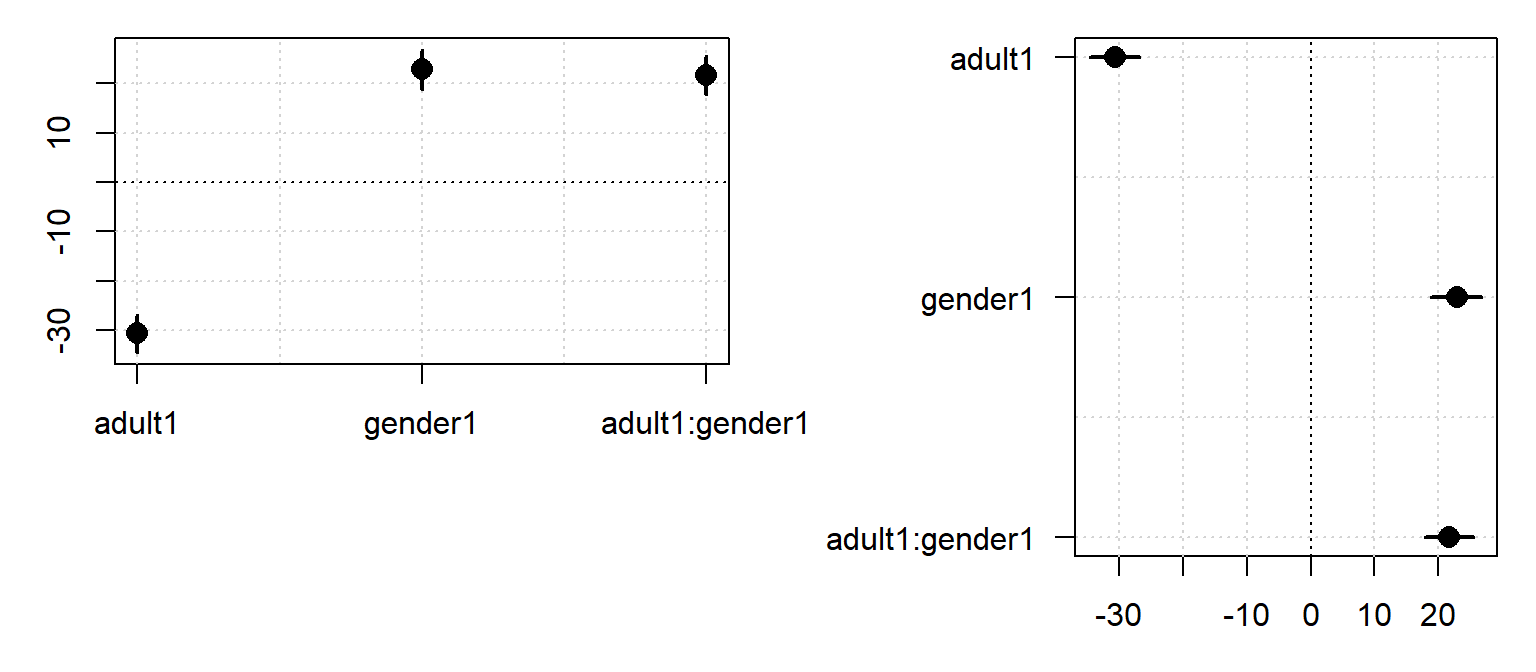
\includegraphics{04_files/figure-latex/brmsplot-1.pdf}
\caption{\label{fig:brmsplot}Horizontal and vertical plots of our fixed effects. Points indicate posterior means and lines indicate span of 95\% credible intervals of the posterior distribution of the parameter.}
\end{figure}

In the left panel below, I use the effects calculated using the \texttt{marginal\_effects} function to draw figures using the \texttt{brmplot} function. First I isolate the columns that represent the information I need. Then I plot the effects using repeated calls to \texttt{brmplot}. I can add a second plot over the first by setting \texttt{add\ =\ TRUE}.

In the right plot, I do the same thing using the output of the hypothesis function. This will be a plot of the group effects centered at 0, since I have not added the overall Intercept to the means. Note that to get the table of interest out of the hypothesis object we have to first select the element named ``hypothesis'' from the \texttt{group\_effects} object. In general, you may have to dig around in the structure of the objects created by \texttt{brms} to get the information you want. I usually run a \texttt{str} on the resulting object to see what's inside it, and what seems likely to contain the information I'm after.

\begin{Shaded}
\begin{Highlighting}[]
\CommentTok{\# estimates of group means based on model coefficients provided}
\CommentTok{\# by the conditional\_effects function.}
\NormalTok{model\_effects[[}\DecValTok{3}\NormalTok{]][,}\DecValTok{8}\SpecialCharTok{:}\DecValTok{11}\NormalTok{]}
\DocumentationTok{\#\#   estimate\_\_     se\_\_  lower\_\_  upper\_\_}
\DocumentationTok{\#\# 1   220.5119 2.950740 214.4826 226.4404}
\DocumentationTok{\#\# 2   131.3351 3.191314 124.9046 137.3878}
\DocumentationTok{\#\# 3   238.4238 4.839866 229.0110 247.6442}
\DocumentationTok{\#\# 4   236.0509 4.175498 227.9085 244.4526}

\CommentTok{\# the same thing is calculated \textquotesingle{}manually\textquotesingle{} using the hypothesis function}
\NormalTok{group\_effects }\OtherTok{=} 
\NormalTok{  brms}\SpecialCharTok{::}\FunctionTok{hypothesis}\NormalTok{ (model\_interaction, }\AttributeTok{hypothesis =} 
                \FunctionTok{c}\NormalTok{(}\StringTok{"{-}adult1 + {-}gender1 +  adult1:gender1 = 0"}\NormalTok{,}
                  \StringTok{"{-}adult1 +  gender1 + {-}adult1:gender1 = 0"}\NormalTok{,}
                  \StringTok{" adult1 + {-}gender1 + {-}adult1:gender1 = 0"}\NormalTok{,}
                  \StringTok{" adult1 +  gender1 +  adult1:gender1 = 0"}\NormalTok{))}
\NormalTok{group\_effects[[}\StringTok{"hypothesis"}\NormalTok{]][,}\DecValTok{2}\SpecialCharTok{:}\DecValTok{5}\NormalTok{]}
\DocumentationTok{\#\#    Estimate Est.Error   CI.Lower  CI.Upper}
\DocumentationTok{\#\# 1  29.49602  3.572487  22.395865  36.55756}
\DocumentationTok{\#\# 2  31.84266  3.942479  24.140857  39.59088}
\DocumentationTok{\#\# 3 {-}75.28023  2.941089 {-}81.039480 {-}69.48480}
\DocumentationTok{\#\# 4  13.94155  2.891922   8.309273  19.62493}
\end{Highlighting}
\end{Shaded}

\begin{Shaded}
\begin{Highlighting}[]
\FunctionTok{par}\NormalTok{ (}\AttributeTok{mfrow =} \FunctionTok{c}\NormalTok{(}\DecValTok{1}\NormalTok{,}\DecValTok{2}\NormalTok{), }\AttributeTok{mar =} \FunctionTok{c}\NormalTok{(}\DecValTok{4}\NormalTok{,}\DecValTok{4}\NormalTok{,}\DecValTok{1}\NormalTok{,}\DecValTok{1}\NormalTok{))}
\FunctionTok{brmplot}\NormalTok{ (model\_effects[[}\DecValTok{3}\NormalTok{]][}\DecValTok{1}\SpecialCharTok{:}\DecValTok{2}\NormalTok{,}\DecValTok{8}\SpecialCharTok{:}\DecValTok{11}\NormalTok{], }\AttributeTok{type =} \StringTok{\textquotesingle{}b\textquotesingle{}}\NormalTok{, }\AttributeTok{ylim =} \FunctionTok{c}\NormalTok{(}\DecValTok{120}\NormalTok{,}\DecValTok{250}\NormalTok{), }
         \AttributeTok{labels=}\FunctionTok{c}\NormalTok{(}\StringTok{"Female"}\NormalTok{,}\StringTok{"Male"}\NormalTok{), }\AttributeTok{col =} \DecValTok{3}\NormalTok{, }\AttributeTok{xlim =} \FunctionTok{c}\NormalTok{(.}\DecValTok{8}\NormalTok{,}\FloatTok{2.2}\NormalTok{))}
\FunctionTok{brmplot}\NormalTok{ (model\_effects[[}\DecValTok{3}\NormalTok{]][}\DecValTok{3}\SpecialCharTok{:}\DecValTok{4}\NormalTok{,}\DecValTok{8}\SpecialCharTok{:}\DecValTok{11}\NormalTok{], }\AttributeTok{type =} \StringTok{\textquotesingle{}b\textquotesingle{}}\NormalTok{, }\AttributeTok{add =} \ConstantTok{TRUE}\NormalTok{, }\AttributeTok{col =} \DecValTok{4}\NormalTok{,}
         \AttributeTok{labels=}\StringTok{""}\NormalTok{, }\AttributeTok{pch=}\DecValTok{17}\NormalTok{)}

\FunctionTok{brmplot}\NormalTok{ (group\_effects[[}\StringTok{"hypothesis"}\NormalTok{]][}\DecValTok{4}\SpecialCharTok{:}\DecValTok{3}\NormalTok{,}\DecValTok{2}\SpecialCharTok{:}\DecValTok{5}\NormalTok{], }\AttributeTok{type =} \StringTok{\textquotesingle{}b\textquotesingle{}}\NormalTok{, }\AttributeTok{ylim =} \FunctionTok{c}\NormalTok{(}\SpecialCharTok{{-}}\DecValTok{85}\NormalTok{,}\DecValTok{40}\NormalTok{),  }
         \AttributeTok{labels=}\FunctionTok{c}\NormalTok{(}\StringTok{"Female"}\NormalTok{,}\StringTok{"Male"}\NormalTok{), }\AttributeTok{col =} \DecValTok{3}\NormalTok{, }\AttributeTok{xlim =} \FunctionTok{c}\NormalTok{(.}\DecValTok{8}\NormalTok{,}\FloatTok{2.2}\NormalTok{))}
\FunctionTok{brmplot}\NormalTok{ (group\_effects[[}\StringTok{"hypothesis"}\NormalTok{]][}\DecValTok{2}\SpecialCharTok{:}\DecValTok{1}\NormalTok{,}\DecValTok{2}\SpecialCharTok{:}\DecValTok{5}\NormalTok{], }\AttributeTok{type =} \StringTok{\textquotesingle{}b\textquotesingle{}}\NormalTok{, }\AttributeTok{add =} \ConstantTok{TRUE}\NormalTok{, }\AttributeTok{col =} \DecValTok{4}\NormalTok{,}
         \AttributeTok{labels=}\StringTok{""}\NormalTok{, }\AttributeTok{pch=}\DecValTok{17}\NormalTok{)}
\end{Highlighting}
\end{Shaded}

\begin{figure}
\centering
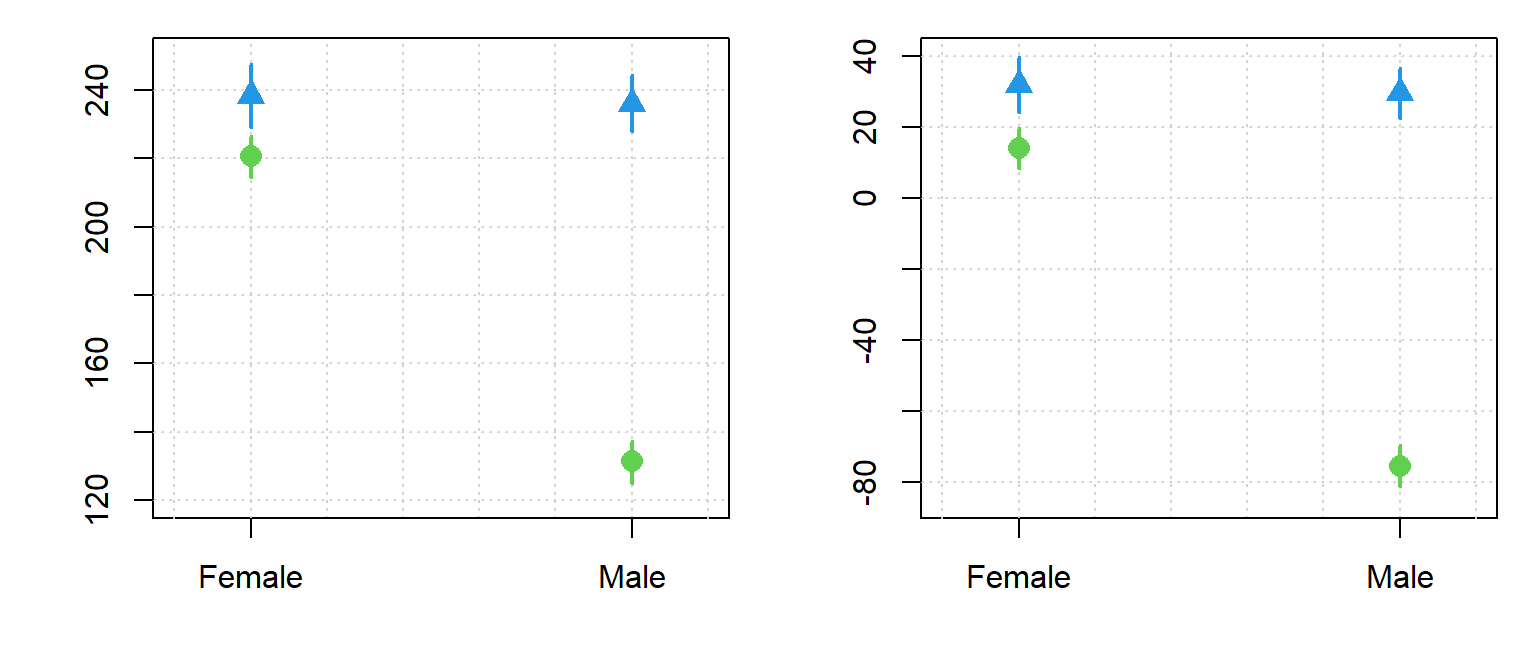
\includegraphics{04_files/figure-latex/brmsplot2-1.pdf}
\caption{\label{fig:brmsplot2}The examples of using parameter summaries to draw plots using the brmplot function.}
\end{figure}

\hypertarget{lmer-corner-1}{%
\section{Lmer corner}\label{lmer-corner-1}}

This is going to be a short one! The main shortcoming when it comes to \texttt{lmer} and fitting ANOVA-type models, is that there is no easy way to compare group effects within the model. For example, we can fit the model below which encodes the difference between each group mean and the overall mean.

\begin{Shaded}
\begin{Highlighting}[]
\NormalTok{lmer\_four\_groups }\OtherTok{=}\NormalTok{ lme4}\SpecialCharTok{::}\FunctionTok{lmer}\NormalTok{ (f0 }\SpecialCharTok{\textasciitilde{}}\NormalTok{ group }\SpecialCharTok{+}\NormalTok{ (}\DecValTok{1}\SpecialCharTok{|}\NormalTok{speaker), }\AttributeTok{data =}\NormalTok{ h95)}
\FunctionTok{summary}\NormalTok{ (lmer\_four\_groups)}
\DocumentationTok{\#\# Linear mixed model fit by REML [\textquotesingle{}lmerMod\textquotesingle{}]}
\DocumentationTok{\#\# Formula: f0 \textasciitilde{} group + (1 | speaker)}
\DocumentationTok{\#\#    Data: h95}
\DocumentationTok{\#\# }
\DocumentationTok{\#\# REML criterion at convergence: 13468.5}
\DocumentationTok{\#\# }
\DocumentationTok{\#\# Scaled residuals: }
\DocumentationTok{\#\#     Min      1Q  Median      3Q     Max }
\DocumentationTok{\#\# {-}4.6436 {-}0.5611 {-}0.0857  0.4703  4.8079 }
\DocumentationTok{\#\# }
\DocumentationTok{\#\# Random effects:}
\DocumentationTok{\#\#  Groups   Name        Variance Std.Dev.}
\DocumentationTok{\#\#  speaker  (Intercept) 429.6    20.73   }
\DocumentationTok{\#\#  Residual             140.6    11.86   }
\DocumentationTok{\#\# Number of obs: 1668, groups:  speaker, 139}
\DocumentationTok{\#\# }
\DocumentationTok{\#\# Fixed effects:}
\DocumentationTok{\#\#             Estimate Std. Error t value}
\DocumentationTok{\#\# (Intercept)  206.511      1.913 107.931}
\DocumentationTok{\#\# group1        29.563      3.440   8.594}
\DocumentationTok{\#\# group2        31.840      3.908   8.147}
\DocumentationTok{\#\# group3       {-}75.293      2.927 {-}25.728}
\DocumentationTok{\#\# }
\DocumentationTok{\#\# Correlation of Fixed Effects:}
\DocumentationTok{\#\#        (Intr) group1 group2}
\DocumentationTok{\#\# group1  0.065              }
\DocumentationTok{\#\# group2  0.287 {-}0.464       }
\DocumentationTok{\#\# group3 {-}0.216 {-}0.286 {-}0.402}
\end{Highlighting}
\end{Shaded}

The results provided by \texttt{lmer} are very similar to those provided by \texttt{brm}:

\begin{Shaded}
\begin{Highlighting}[]
\NormalTok{brms}\SpecialCharTok{::}\FunctionTok{fixef}\NormalTok{ (model\_four\_groups)}
\DocumentationTok{\#\#            Estimate Est.Error      Q2.5     Q97.5}
\DocumentationTok{\#\# Intercept 206.48607  1.928704 202.66968 210.21349}
\DocumentationTok{\#\# group1     29.53202  3.523919  22.78309  36.64507}
\DocumentationTok{\#\# group2     31.87791  3.976443  24.35103  39.68355}
\DocumentationTok{\#\# group3    {-}75.17590  2.903665 {-}80.88864 {-}69.61975}
\end{Highlighting}
\end{Shaded}

Group 1 (boys) and group 2 (girls) have very similar effects to each other. Are they different? Using our \texttt{brm} model this can be answered easily, as shown above (and reproduced below):

\begin{Shaded}
\begin{Highlighting}[]
\NormalTok{brms}\SpecialCharTok{::}\FunctionTok{hypothesis}\NormalTok{ (model\_four\_groups, }\StringTok{"group2 {-} group1 = 0"}\NormalTok{)[[}\DecValTok{1}\NormalTok{]][,}\DecValTok{1}\SpecialCharTok{:}\DecValTok{5}\NormalTok{]}
\DocumentationTok{\#\#            Hypothesis Estimate Est.Error  CI.Lower CI.Upper}
\DocumentationTok{\#\# 1 (group2{-}group1) = 0 2.345888  6.437511 {-}10.28229 15.03817}
\end{Highlighting}
\end{Shaded}

Unfortunately, there is no way to answer this question given the information presented in the \texttt{lmer} model above. This is because the effects are only being estimates as differences to the mean, and not to group 1 or group 2). If we \emph{did} want to investigate this difference specifically, we would need to refit the model using a different coding scheme. For example, if we used treatment coding group 1 (boys) would be the intercept, and the group effects would represent differences to this. We fit a model like this below:

\begin{Shaded}
\begin{Highlighting}[]
\FunctionTok{options}\NormalTok{ (}\AttributeTok{contrasts =} \FunctionTok{rep}\NormalTok{(}\StringTok{"contr.treatment"}\NormalTok{,}\DecValTok{2}\NormalTok{))}
\NormalTok{lmer\_four\_groups\_treatment }\OtherTok{=}\NormalTok{ lme4}\SpecialCharTok{::}\FunctionTok{lmer}\NormalTok{ (f0 }\SpecialCharTok{\textasciitilde{}}\NormalTok{ group }\SpecialCharTok{+}\NormalTok{ (}\DecValTok{1}\SpecialCharTok{|}\NormalTok{speaker), }\AttributeTok{data =}\NormalTok{ h95)}
\FunctionTok{summary}\NormalTok{ (lmer\_four\_groups\_treatment)}
\DocumentationTok{\#\# Linear mixed model fit by REML [\textquotesingle{}lmerMod\textquotesingle{}]}
\DocumentationTok{\#\# Formula: f0 \textasciitilde{} group + (1 | speaker)}
\DocumentationTok{\#\#    Data: h95}
\DocumentationTok{\#\# }
\DocumentationTok{\#\# REML criterion at convergence: 13465.7}
\DocumentationTok{\#\# }
\DocumentationTok{\#\# Scaled residuals: }
\DocumentationTok{\#\#     Min      1Q  Median      3Q     Max }
\DocumentationTok{\#\# {-}4.6436 {-}0.5611 {-}0.0857  0.4703  4.8079 }
\DocumentationTok{\#\# }
\DocumentationTok{\#\# Random effects:}
\DocumentationTok{\#\#  Groups   Name        Variance Std.Dev.}
\DocumentationTok{\#\#  speaker  (Intercept) 429.6    20.73   }
\DocumentationTok{\#\#  Residual             140.6    11.86   }
\DocumentationTok{\#\# Number of obs: 1668, groups:  speaker, 139}
\DocumentationTok{\#\# }
\DocumentationTok{\#\# Fixed effects:}
\DocumentationTok{\#\#             Estimate Std. Error t value}
\DocumentationTok{\#\# (Intercept)  236.074      4.043  58.391}
\DocumentationTok{\#\# groupg         2.277      6.291   0.362}
\DocumentationTok{\#\# groupm      {-}104.856      5.114 {-}20.504}
\DocumentationTok{\#\# groupw       {-}15.673      5.054  {-}3.101}
\DocumentationTok{\#\# }
\DocumentationTok{\#\# Correlation of Fixed Effects:}
\DocumentationTok{\#\#        (Intr) groupg groupm}
\DocumentationTok{\#\# groupg {-}0.643              }
\DocumentationTok{\#\# groupm {-}0.791  0.508       }
\DocumentationTok{\#\# groupw {-}0.800  0.514  0.632}
\end{Highlighting}
\end{Shaded}

Notice that our group 2 predictor (\texttt{group}) is now equal to 2.3, the Hz difference between boys and girls. The value of the standard error (\texttt{Std.\ Error}) is 6.3, representing the uncertainty in the estimate. These values correspond closely to the estimates provided by our Bayesian model above of 2.3 and 6.4 respectively.

Obviously this situation is not ideal if you plan to compare many groups. In contrast, with our \texttt{brm} model we can easily compare any of the four groups using the method outlined above, without ever having to re-fit the model.

\hypertarget{exercises-3}{%
\section{Exercises}\label{exercises-3}}

\hypertarget{including-continuous-predictors-in-our-model}{%
\chapter{Including continuous predictors in our model}\label{including-continuous-predictors-in-our-model}}

Last chapter we talked about comparing many groups, and including interactions in our models. So far we have only discussed models that include nominal predictors. In this chapter we're going to talk about including continuous, numerical predictors in our models.

Just as in chapter 1, we're going to begin by talking about `single' level (\emph{not} multi-level) models. These models have no random effects, and so are not really appropriate for our data. We're going to focus on the interpretation of model coefficients and what these mean for the geometry of the lines we make. Next chapter we'll extend these concepts to understand `random slopes and intercepts' for variables such as speaker and listener.

\hypertarget{data-and-research-questions-4}{%
\section{Data and research questions}\label{data-and-research-questions-4}}

We're still going to work with the Hillenbrand et al.~data, again focusing on variation in f0. We are going to be focusing on a subset of these (productions of ``heed'' and ``hod'' only), produced by all 136 speakers in the data.

Our data has a new continuous variable (\texttt{pheight}) representing the average perceived height for each talker, for each token. In this chapter, we are going to use perceived height as a predictor to see if it can be used to predict the f0 of a token.

\begin{Shaded}
\begin{Highlighting}[]
\FunctionTok{library}\NormalTok{ (brms)}
\FunctionTok{options}\NormalTok{ (}\AttributeTok{contrasts =} \FunctionTok{c}\NormalTok{(}\StringTok{"contr.sum"}\NormalTok{,}\StringTok{"cont.sum"}\NormalTok{))}

\NormalTok{url1 }\OtherTok{=} \StringTok{"https://raw.githubusercontent.com/santiagobarreda"}
\NormalTok{url2 }\OtherTok{=} \StringTok{"/stats{-}class/master/data/h95\_experiment\_summary.csv"}
\NormalTok{h95 }\OtherTok{=} \FunctionTok{read.csv}\NormalTok{ (}\FunctionTok{url}\NormalTok{(}\FunctionTok{paste0}\NormalTok{ (url1, url2)))}
\CommentTok{\# set up colors for plotting}
\NormalTok{devtools}\SpecialCharTok{::}\FunctionTok{source\_url}\NormalTok{ (}\FunctionTok{paste0}\NormalTok{ (url1, }\StringTok{"/stats{-}class/master/data/colors.R"}\NormalTok{))}
\CommentTok{\# source functions}
\NormalTok{devtools}\SpecialCharTok{::}\FunctionTok{source\_url}\NormalTok{ (}\FunctionTok{paste0}\NormalTok{ (url1, }\StringTok{"/stats{-}class/master/data/functions.R"}\NormalTok{))}

\CommentTok{\# make group a factor}
\NormalTok{h95}\SpecialCharTok{$}\NormalTok{group }\OtherTok{=} \FunctionTok{factor}\NormalTok{ (h95}\SpecialCharTok{$}\NormalTok{group)  }
\end{Highlighting}
\end{Shaded}

\hypertarget{continuous-predictors-modeling-variation-along-lines}{%
\section{Continuous predictors: modeling variation along lines}\label{continuous-predictors-modeling-variation-along-lines}}

Below I plot the average f0 for each token against its average perceived height in inches. I use a scatter plot with the dependent variable (\texttt{f0}, the thing we are interested in) varying along the y axis (this is done by convention).

The scatter plot clearly shows what is called a \emph{linear relationship} between the two variables. As far as we're concerned, this just means when you make a scatter plot, you will see points you think are suggestive of a line, or a couple of lines.

Our models have so far featured only nominal predictors, things like group membership. Although it might be strange to think of it this way, our regression models \emph{have} been making lines, however, they are lines with slopes of 0 along all x axis variables. What this means is, that for any x-axis variable, variation along the x axis variable \textbf{has no effect} on variation along the y axis variable.

Below I show an example of what I mean by this. Figure \ref{fig:F5-fig1} shows several an `intercept only model' that features a fixed f0 for all tokens. In the right panel I show four lines, one for each group. These lines have different intercept but have the same slope (0). This means that these lines try to predict f0 based on group, but do not allow this to vary as a function of perceived height.

When we look at lines such as those below, they tell us that our model thinks mean f0 is \emph{independent} of perceived height. This is because perceived height can vary from positive to negative infinity and we don't expect f0 to change (the line is flat!). The same statement could be made for any x variable we chose because our model does not include slopes for \emph{any} variable.

\begin{figure}
\centering
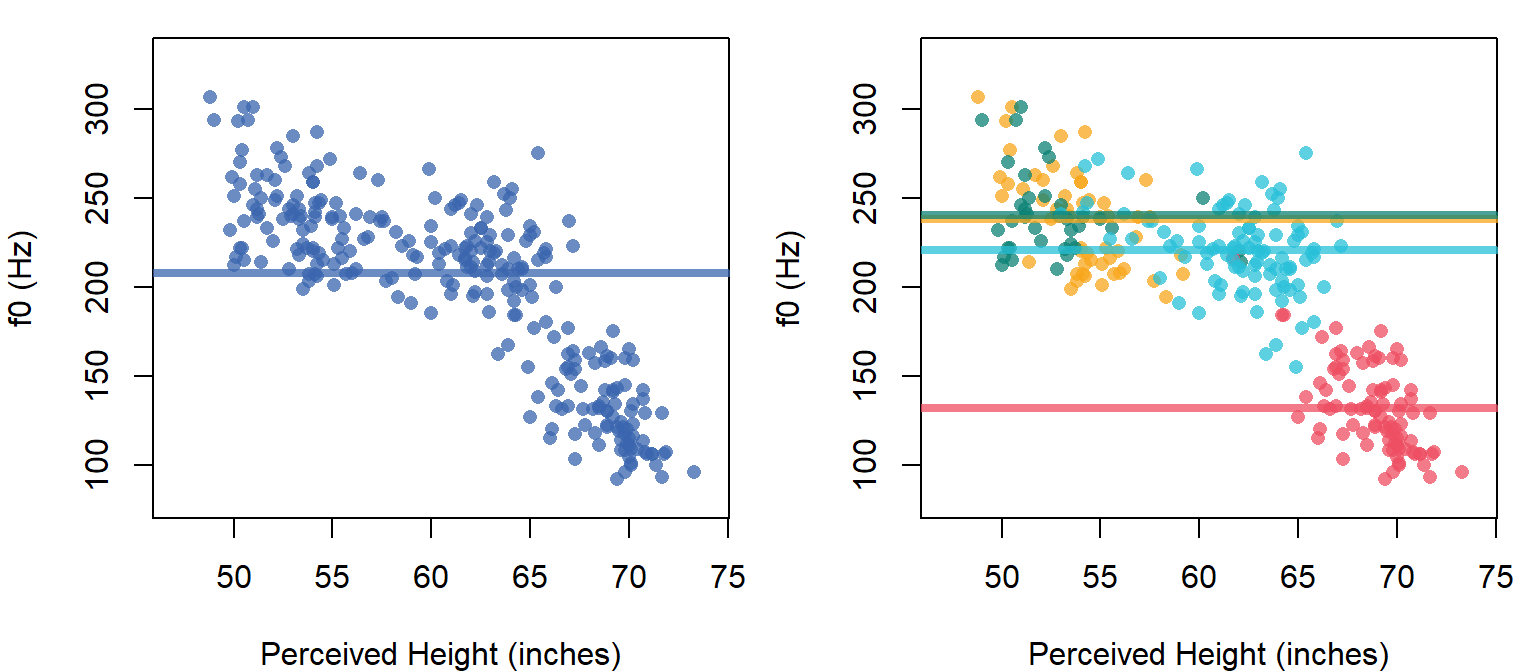
\includegraphics{05_files/figure-latex/F5-fig1-1.pdf}
\caption{\label{fig:F5-fig1}(left) f0 plotted against perceived height for each token. Horizontal line is the mean of the group means. (right) Same as right panel except each group gets its own horizontal line. Groups are boys (yellow), girls (green), women (blue), and men (red).}
\end{figure}

Recall that the equation for a line is the following:

\[
y = m*x + b \\ 
\label{eq:51}
\]

Where \(y\) is the `output' variable you are `predicting' using a line with a slope of \(m\) and and intercept of \(b\). The slope \(m\) represents how much of a change you expect in your \(y\) variable for a \emph{1 unit change} in your x variable. Obviously, this means that the slope depends on the units of measurement of your \(x\) variable. In general, dividing your \(x\) predictor by \(z\) will increase your slopes by a factor of \(z\). For example, imagine measuring the slope of a long hill with a constant rise. The amount of rise over 1 meter will necessarily be 1/1000 as much as the amount of rise over one kilometer.

We can use the following line equation, which just uses symbols that are more similar to the ones we have been using (and presents them in a different order):

\[
\mu = a + b*x \\
\label{eq:52}
\]

We can predict f0 in the left panel of Figure \ref{fig:F5-fig1} using a horizontal line by setting the intercept to the overall grand mean, and setting the slope coefficient to 0. In this case we would have an `intercept only' regression model just like the one we saw in chapters 1 and 2.

\[
a = Intercept, b = 0 \\ \\
f0 = Intercept = Intercept + 0*pheight \\
\label{eq:53}
\]

In the right panel of Figure \ref{fig:F5-fig1} we see four horizontal lines, one for each group of speakers. These lines all differ in terms of intercept but have the same slope (0). This means that these lines try to predict f0 based on group, but don't allow this to vary as a function of perceived height. So, our four-group model with only nominal predictors in chapter 4 could really be thought of as predicting f0 along a set of lines that are horizontal along the perceived height dimension.

\[
a = Intercept + group_{[\mathrm{group}]}, b = 0 \\ \\
f0 = Intercept + group_{[\mathrm{group}]} + (0*pheight) \\
\label{eq:56}
\]

Ok, so what if we \emph{do} want to think about variation in f0 as a function of variation in perceived height. In Figure \ref{fig:F5-52} we can see what this might look like. On the left we have a normal distribution sliding along a horizontal line, generating numbers as it slides. The mean of this data does not vary based on the values of perceived height, and so is \emph{independent} of them. The standard deviation of this distribution (\(\sigma_{error}\)) does not not change as a function of perceived height so its `width' is stable.

On the right in Figure \ref{fig:F5-52} we can imagine that the mean of the normal distribution generating f0 values \emph{does} change as a function of the value of perceived height. We can say that the model on the right predicts f0 \emph{conditional on} values of perceived height.

The model on the right in Figure \ref{fig:F5-52} places an important constraint on this conditional variation: the mean of f0 varies strictly along a straight line. So, to predict f0 given a certain perceived height, we slide our normal distribution along long the diagonal line in Figure \ref{fig:F5-52} to the proper x axis location. The y axis value of the line at this x axis location represents our predicted value (\(\mu\)). The actual value of observations would then vary around this expected value in a normal distribution with a mean of 0 and a standard deviation equal to \(\sigma_{error}\).

\begin{figure}
\centering
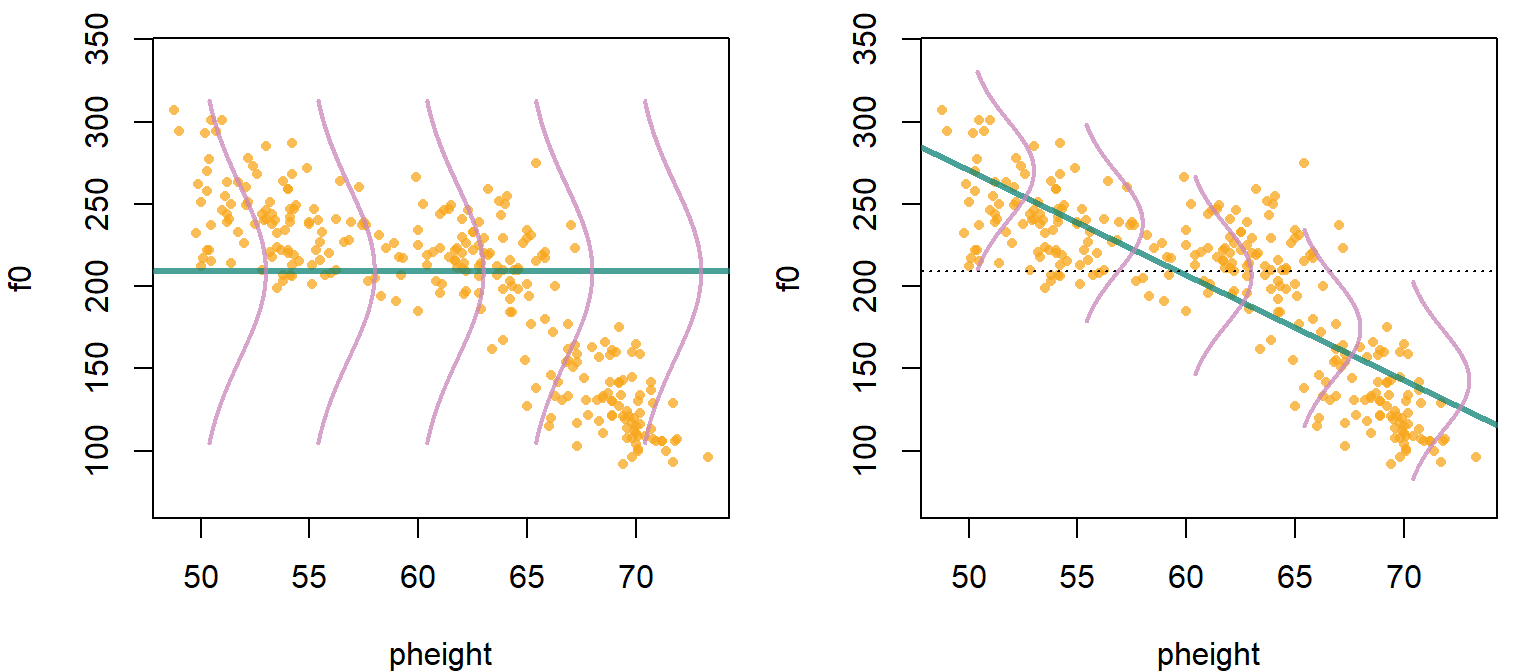
\includegraphics{05_files/figure-latex/F5-52-1.pdf}
\caption{\label{fig:F5-52}(left) A normal distribution fixed along a horizontal line. (right) A Normal distribution allowed to slide along a diagonal line.}
\end{figure}

\hypertarget{models-with-a-single-slope-and-intercept}{%
\section{Models with a single slope and intercept}\label{models-with-a-single-slope-and-intercept}}

We can use the \texttt{brm} function to find the intercept and slope of the `best' line through the points in our two-dimensional space (represented in the scatter plot). Our model formula will look like this:

\texttt{f0\ \textasciitilde{}\ pheight}

Which tells \texttt{brms} to predict \texttt{f0} based on the values of \texttt{pheight}. If the variable on the right hand side of the \texttt{\textasciitilde{}} is numeric, \texttt{brm} will treat it as a continuous predictor and predict f0 using a line.

\hypertarget{description-of-the-model-4}{%
\subsection{Description of the model}\label{description-of-the-model-4}}

Our model for a regression model with a single continuous predictor (a `bivariate' regression) is shown below. The first line says that we have a normally-distributed variable with an unknown mean that varies from trial to trial (\(\mu_{[i]}\)). The variation in the mean parameter varies along a line with an intercept equal to \(Intercept\) and a slope of \(pheight\) along the x axis.

Note that the predicted value (\(\mu_{[i]}\)) and the predictor variable (\(x_{[i]}\)) receive subscripts, as these change from trial to trial. The coefficients \textbf{do not} receive subscripts because these do not vary in this model. This model contains a single intercept and a single slope (i.e.~it draws a single line) for \emph{every} trial. Also note that we're simply treating the slope and intercept as `fixed' effects and specifying prior distributions.

\begin{equation}
\begin{split}
\\
\textrm{Likelihood:} \\
y_{[i]} \sim \mathcal{N}(\mu_{[i]},\sigma_{error}) \\
\mu_{[i]} = Intercept + pheight * x_{[i]}  \\ \\
\textrm{Priors:} \\
Intercept \sim t(3, 175, 100) \\
pheight \sim t(3, 0, 100) \\
\\
\end{split}
\label{eq:57}
\end{equation}

Here's another two ways to think about this model: we're making a line and add noise to it. Each of our observed values is just a line (representing systematic variation) and a random draw from an error distribution (\(\mathcal{N}(0,\sigma_{error})\)).

\[
y_{[i]} = a + b * \mathrm{x_{[i]}} + \mathcal{N}(0,\sigma_{error})
\label{eq:58}
\]

Alternatively, we could place the formula for the line \emph{inside} the formula for the normal distribution. There is no particular reason to do this, but it is helpful to see it and realize that it's the same thing as the representation above. In the equation below, we're saying: the data is generated according to a normal distribution whose mean varies along a line (\(a + b * \mathrm{x_{[i]}}\)), and we expect the variation around this line to have a standard deviation equal to \(\sigma_{error}\).

\[
\mathcal{N}(a + b * \mathrm{x_{[i]}}, \sigma_{error})  \\
\label{eq:59}
\]

Regression models pick the intercept and slope for a line that results in the smallest value of \(\sigma_{error}\). This is why `regular' regression is called \href{https://en.wikipedia.org/wiki/Ordinary_least_squares}{``ordinary least-squares''} regression, because it finds the solution that results in the `least squares' (i.e., the smallest \((\sigma_{error})^2\)) in the prediction errors.

In a multilevel model, the estimation of the `best' slopes and intercepts for our lines can be substantially more complicated than in least-squares regression. For example, in the case of experiments these estimates would take within and between-participant variation into account. However, in general the lines estimated by our regression models will tend to minimize the value of \(\sigma_{error}\), given our data and model structure.

\hypertarget{fitting-the-model-3}{%
\subsection{Fitting the model}\label{fitting-the-model-3}}

We can use the \texttt{brm} function to find the intercept and slope of the `best' line through the points in our two-dimensional space (represented in the scatter plot).

\begin{Shaded}
\begin{Highlighting}[]
\FunctionTok{options}\NormalTok{ (}\AttributeTok{contrasts =} \FunctionTok{c}\NormalTok{(}\StringTok{"contr.sum"}\NormalTok{,}\StringTok{"cont.sum"}\NormalTok{))}
\CommentTok{\# Fit the model yourself, or}
\CommentTok{\# download pre{-}fit model from: }
\CommentTok{\# github.com/santiagobarreda/stats{-}class/tree/master/models}
\CommentTok{\# and load after placing in working directory}
\CommentTok{\# single\_line\_model = readRDS (\textquotesingle{}5\_single\_line\_model.RDS\textquotesingle{})}

\FunctionTok{set.seed}\NormalTok{ (}\DecValTok{1}\NormalTok{)}
\NormalTok{single\_line\_model }\OtherTok{=}
  \FunctionTok{brm}\NormalTok{ (f0 }\SpecialCharTok{\textasciitilde{}}\NormalTok{ pheight, }\AttributeTok{data =}\NormalTok{ h95, }\AttributeTok{chains=}\DecValTok{1}\NormalTok{, }\AttributeTok{cores=}\DecValTok{1}\NormalTok{,  }\AttributeTok{warmup=}\DecValTok{1000}\NormalTok{, }\AttributeTok{iter =} \DecValTok{6000}\NormalTok{,}
       \AttributeTok{prior =} \FunctionTok{c}\NormalTok{(}\FunctionTok{set\_prior}\NormalTok{(}\StringTok{"student\_t(3, 175, 100)"}\NormalTok{, }\AttributeTok{class =} \StringTok{"Intercept"}\NormalTok{),}
                 \FunctionTok{set\_prior}\NormalTok{(}\StringTok{"student\_t(3, 0, 100)"}\NormalTok{, }\AttributeTok{class =} \StringTok{"b"}\NormalTok{)))}
\CommentTok{\# save model}
\CommentTok{\# saveRDS (single\_line\_model, \textquotesingle{}5\_single\_line\_model.RDS\textquotesingle{})}
\end{Highlighting}
\end{Shaded}

\hypertarget{interpreting-the-model-2}{%
\subsection{Interpreting the model}\label{interpreting-the-model-2}}

The model print statement is mostly the same as for our previous models. Our model contains only `fixed' effects: an \texttt{Intercept}, indicating the intercept of our line, and \texttt{pheight} indicating the slope of f0 along the perceived height axis. We get credible intervals for our slope coefficient, and our model features an estimate of the error (\texttt{sigma}, \(\sigma_{error}\)) around our line.

\begin{Shaded}
\begin{Highlighting}[]
\CommentTok{\# inspect model}
\NormalTok{single\_line\_model}
\DocumentationTok{\#\#  Family: gaussian }
\DocumentationTok{\#\#   Links: mu = identity; sigma = identity }
\DocumentationTok{\#\# Formula: f0 \textasciitilde{} pheight }
\DocumentationTok{\#\#    Data: h95 (Number of observations: 278) }
\DocumentationTok{\#\# Samples: 1 chains, each with iter = 6000; warmup = 1000; thin = 1;}
\DocumentationTok{\#\#          total post{-}warmup samples = 5000}
\DocumentationTok{\#\# }
\DocumentationTok{\#\# Population{-}Level Effects: }
\DocumentationTok{\#\#           Estimate Est.Error l{-}95\% CI u{-}95\% CI Rhat Bulk\_ESS Tail\_ESS}
\DocumentationTok{\#\# Intercept   588.68     16.42   556.41   620.73 1.00     5261     3935}
\DocumentationTok{\#\# pheight      {-}6.36      0.27    {-}6.89    {-}5.84 1.00     5283     3962}
\DocumentationTok{\#\# }
\DocumentationTok{\#\# Family Specific Parameters: }
\DocumentationTok{\#\#       Estimate Est.Error l{-}95\% CI u{-}95\% CI Rhat Bulk\_ESS Tail\_ESS}
\DocumentationTok{\#\# sigma    30.21      1.31    27.78    32.93 1.00     4562     3693}
\DocumentationTok{\#\# }
\DocumentationTok{\#\# Samples were drawn using sampling(NUTS). For each parameter, Bulk\_ESS}
\DocumentationTok{\#\# and Tail\_ESS are effective sample size measures, and Rhat is the potential}
\DocumentationTok{\#\# scale reduction factor on split chains (at convergence, Rhat = 1).}
\end{Highlighting}
\end{Shaded}

We can see that the line predicting perceived height as a function of f0 has an intercept of 589 and a slope for the \texttt{pheight} (perceived height) predictor of -6.4. The fact that the slope of the \texttt{pheight} predictor is -6.4 means that for every 1 inch increase in perceived height, we expect a \emph{decrease} of 6.4 Hz in f0. I draw this line on our set of points in Figure \ref{fig:F5-53}.

The slope is a \emph{weight} that allows the line to accurately fit the points. In the absence of a slope, regression models would only work if there was a 1 to 1 relationship between the x and y variables. This would mean that for every 1 inch change in perceived height, we would see a 1 Hz change in f0. What are the odds of that? What are the odds that the things we measure will be in a 1 to 1 relationship like that in general? The odds are basically zero.

Instead, the slope (\(b\) coefficient) on regression models allows a single unit change in the predictor to be associated with different units of change in the \(y\) variable. In this case, a 1 unit change in perceived height (measured in inches) is associated with a 6 unit change in f0 (measured in Hz).

\begin{figure}
\centering
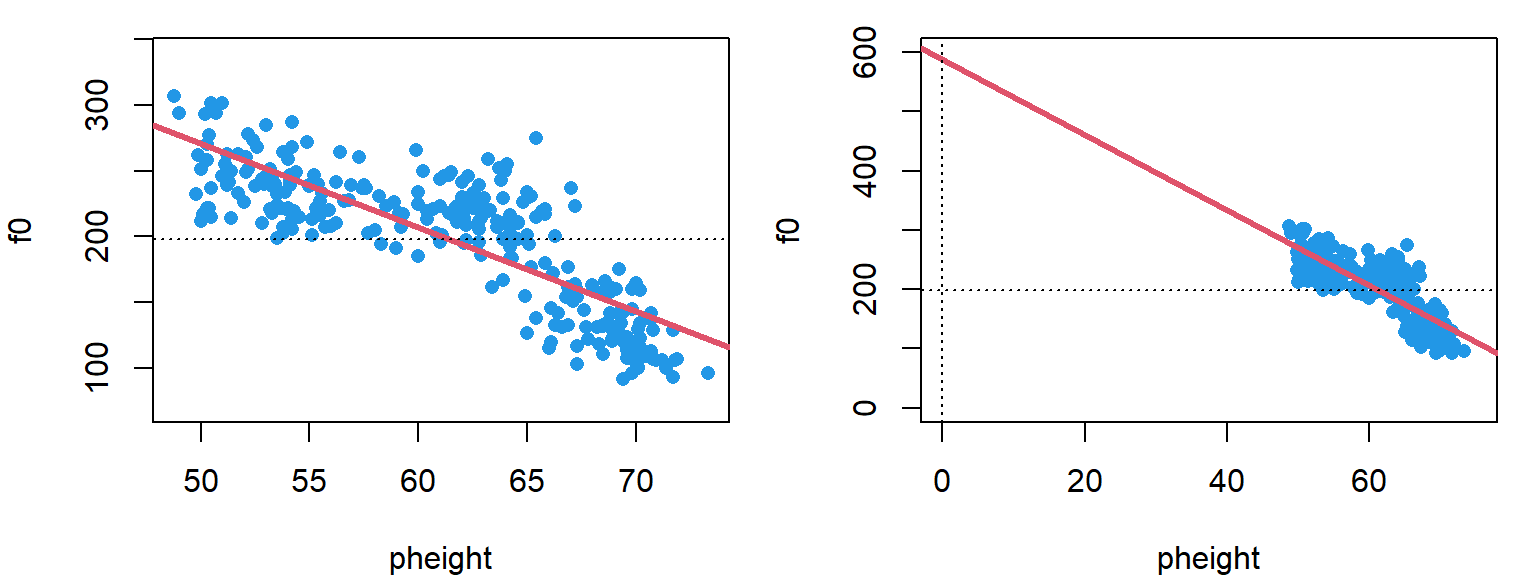
\includegraphics{05_files/figure-latex/F5-53-1.pdf}
\caption{\label{fig:F5-53}(left) Points and best-fit line. (right) A zoomed-out view of the left panel shows the line intercept at y = 588.7 Hz.}
\end{figure}

The intercept is the value of your dependent variable (\(y\), the variable you are interested in) when your predictor is equal to 0. In our model, this means that the expected value of f0 is 588 Hz when the predicted height is 0 inches. These are not particularly meaningful values for either variable as the f0 is too high and people are never 0 inches tall. However, in the right panel of Figure \ref{fig:F5-53} we can see why we get this value: it is simply the y-axis ``intercept'' (zero crossing) of the line we drew through the points in the left panel.

\hypertarget{centering-predictors}{%
\subsection{Centering predictors}\label{centering-predictors}}

We can get more useful intercept values by simply centering our predictor variable(s). Centering a variable means subtracting the mean value from all observations. When this is done, each observation will now represent a deviation from 0, and the sum (and mean) of all the observations will equal zero. Since the intercept of the line is the value of the \(y\) variable when the \(x\) variable is equal to zero, centering our predictor makes the intercept equal to the value of \(y\) when \(x\) is equal to its zero, its mean.

Centering predictor variables affects that intercept of the model but does does not affect the model slope or error estimates. Thus, centering is basically like choosing the `coding' (e.g., sum coding vs.~dummy coding) for lines, it affects how the information is represented in the model, but not the information itself. As a result, it can be tremendously useful in yielding more interpretable intercept estimates. Below, I center perceived height and again predict f0 based on this value.

\begin{Shaded}
\begin{Highlighting}[]
\CommentTok{\# find mean perceived height}
\NormalTok{mean\_perceived\_height }\OtherTok{=} \FunctionTok{mean}\NormalTok{(h95}\SpecialCharTok{$}\NormalTok{pheight)}
\NormalTok{mean\_perceived\_height}
\DocumentationTok{\#\# [1] 61.38813}

\CommentTok{\# center perceived height}
\NormalTok{h95}\SpecialCharTok{$}\NormalTok{pheight\_c }\OtherTok{=}\NormalTok{ h95}\SpecialCharTok{$}\NormalTok{pheight }\SpecialCharTok{{-}}\NormalTok{ mean\_perceived\_height}
\end{Highlighting}
\end{Shaded}

\begin{Shaded}
\begin{Highlighting}[]
\CommentTok{\# Fit the model yourself, or}
\CommentTok{\# download pre{-}fit model from: }
\CommentTok{\# github.com/santiagobarreda/stats{-}class/tree/master/models}
\CommentTok{\# and load after placing in working directory}
\CommentTok{\# single\_line\_model = readRDS (\textquotesingle{}5\_single\_line\_centered\_model.RDS\textquotesingle{})}

\FunctionTok{set.seed}\NormalTok{ (}\DecValTok{1}\NormalTok{)}
\NormalTok{single\_line\_centered\_model }\OtherTok{=}
  \FunctionTok{brm}\NormalTok{ (f0 }\SpecialCharTok{\textasciitilde{}}\NormalTok{ pheight\_c, }\AttributeTok{data=}\NormalTok{h95, }\AttributeTok{chains=}\DecValTok{1}\NormalTok{,}\AttributeTok{cores=}\DecValTok{1}\NormalTok{,}\AttributeTok{warmup=}\DecValTok{1000}\NormalTok{,}\AttributeTok{iter=}\DecValTok{6000}\NormalTok{,}
       \AttributeTok{prior =} \FunctionTok{c}\NormalTok{(}\FunctionTok{set\_prior}\NormalTok{(}\StringTok{"student\_t(3, 175, 100)"}\NormalTok{, }\AttributeTok{class =} \StringTok{"Intercept"}\NormalTok{),}
                 \FunctionTok{set\_prior}\NormalTok{(}\StringTok{"student\_t(3, 0, 100)"}\NormalTok{, }\AttributeTok{class =} \StringTok{"b"}\NormalTok{)))}
\CommentTok{\# save model}
\CommentTok{\# saveRDS (single\_line\_centered\_model, \textquotesingle{}5\_single\_line\_centered\_model.RDS\textquotesingle{})}
\end{Highlighting}
\end{Shaded}

\begin{Shaded}
\begin{Highlighting}[]
\CommentTok{\# inspect model}
\NormalTok{single\_line\_centered\_model}
\DocumentationTok{\#\#  Family: gaussian }
\DocumentationTok{\#\#   Links: mu = identity; sigma = identity }
\DocumentationTok{\#\# Formula: f0 \textasciitilde{} pheight\_centered }
\DocumentationTok{\#\#    Data: h95 (Number of observations: 278) }
\DocumentationTok{\#\# Samples: 1 chains, each with iter = 6000; warmup = 1000; thin = 1;}
\DocumentationTok{\#\#          total post{-}warmup samples = 5000}
\DocumentationTok{\#\# }
\DocumentationTok{\#\# Population{-}Level Effects: }
\DocumentationTok{\#\#                  Estimate Est.Error l{-}95\% CI u{-}95\% CI Rhat Bulk\_ESS Tail\_ESS}
\DocumentationTok{\#\# Intercept          197.99      1.77   194.53   201.53 1.00     6644     4267}
\DocumentationTok{\#\# pheight\_centered    {-}6.37      0.27    {-}6.89    {-}5.84 1.00     4595     3507}
\DocumentationTok{\#\# }
\DocumentationTok{\#\# Family Specific Parameters: }
\DocumentationTok{\#\#       Estimate Est.Error l{-}95\% CI u{-}95\% CI Rhat Bulk\_ESS Tail\_ESS}
\DocumentationTok{\#\# sigma    30.19      1.28    27.86    32.86 1.00     5753     4025}
\DocumentationTok{\#\# }
\DocumentationTok{\#\# Samples were drawn using sampling(NUTS). For each parameter, Bulk\_ESS}
\DocumentationTok{\#\# and Tail\_ESS are effective sample size measures, and Rhat is the potential}
\DocumentationTok{\#\# scale reduction factor on split chains (at convergence, Rhat = 1).}
\end{Highlighting}
\end{Shaded}

We can see that the slope coefficient provided by this model is the same as the last model: the slope of the line has not changed. However, our intercept value is now 198. This means that when out predictor is at its mean (61.4 inches), we expect f0 to have a value of 198 Hz.

\begin{figure}
\centering
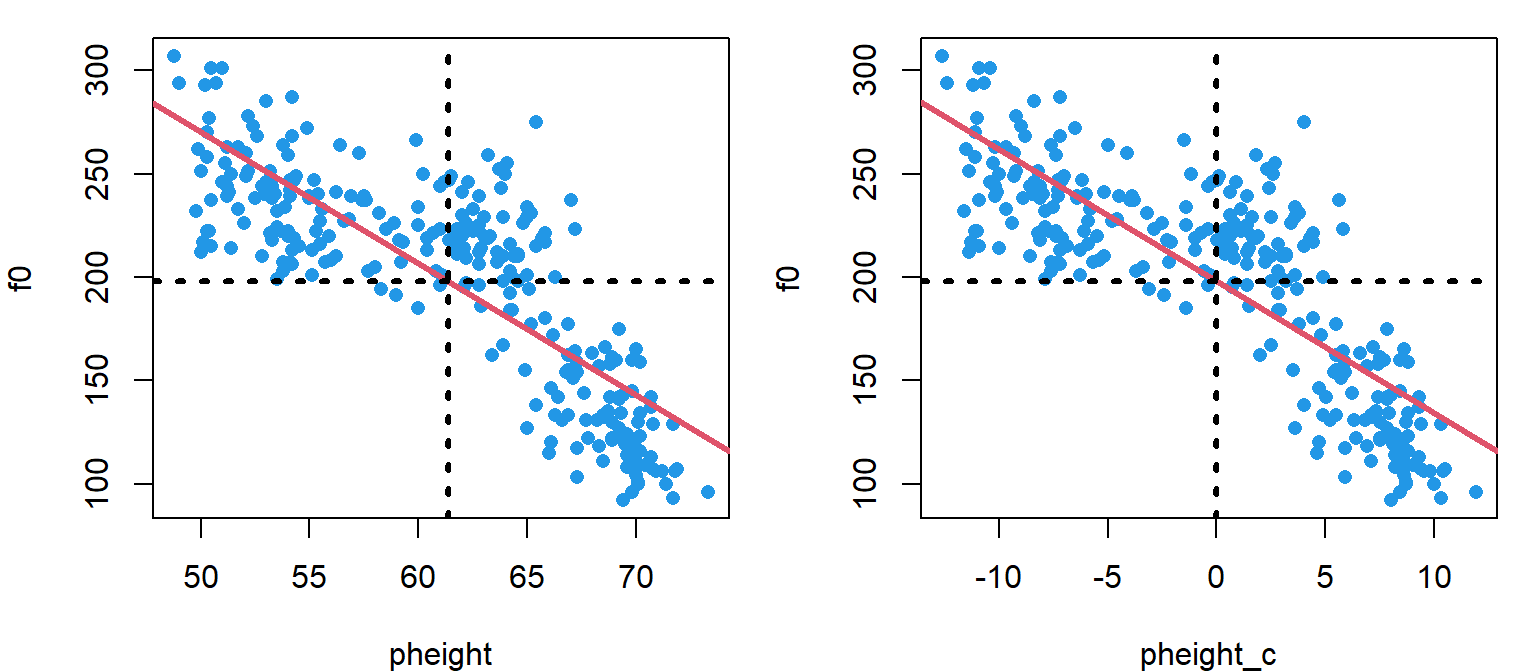
\includegraphics{05_files/figure-latex/F5-slope-n-centered-1.pdf}
\caption{\label{fig:F5-slope-n-centered}(left) Best fit line for points predicted by perceived height. Horizontal and vertical lines indicated y and x variable means respectively. (right) Same as left but with a centered predictor.}
\end{figure}

I'm going to center predictors often, simply out of convenience. However, the decision whether to center or not should really be based on the information you hope to get out of your model, just like the decision of which coding system to use for nominal variables.

\hypertarget{interactions-in-our-line-parameters}{%
\section{Interactions in our line parameters}\label{interactions-in-our-line-parameters}}

Here's something that I haven't really mentioned so far: group effects such as `boy' and `girl' are effectively `interaction' terms. Remember that interactions are \emph{conditional} effects. So, when we say ``hey what's the intercept on the horizontal line you use to model f0?'', the answer is actually ``it depends on the group'' (as seen in Figure @ref:(fig:F5-fig1)). In other words, the intercept in our model is conditional on group. so, when we fit a model like:

\texttt{f0\ \textasciitilde{}\ group}

The model could be thought of as something like:

\texttt{f0\ \textasciitilde{}\ Intercept\ +\ Intercept:group}

This is because our model will estimate a `main effects' (average) intercept term, and also estimate group-dependent deviations from the main effect (i.e., the \texttt{Intercept:group} interactions). By convention, we don't actually specify our models like this, however, it's useful to keep this perspective in mind when thinking about the lines defined by our models.

A nominal predictor like \texttt{group} has the effect of allowing for group-specific intercepts in our lines. Consider what happens when a continuous predictor like \texttt{pheight} is added to our model formula:

\texttt{f0\ \textasciitilde{}\ group\ +\ pheight} (or in our expanded format \texttt{f0\ \textasciitilde{}\ Intercept\ +\ Intercept:group\ +\ pheight})

This model only includes a slope `main effect', or an \emph{average} slope effects across all groups. We can see this because the formula does not contain any interactions with our continuous predictor \texttt{pheight}. As a result, the model does not include any way for the \texttt{pheight} slope to vary (e.g., between groups).

In the last chapter we discussed the fact that without interactions, shared slopes lead to parallel lines in interaction plots. The same applies here! If we draw a bunch of lines with different intercepts but a fixed slope, clearly these lines will all be parallel.

If you want to know about the slope \emph{conditional} on group, then you need to include a group by slope interaction in your model. We add this to out model formula:

\texttt{f0\ \textasciitilde{}\ group\ *\ pheight} or \texttt{f0\ \textasciitilde{}\ group\ +\ pheight\ +\ pheight:group}

Which could be expanded like this:

\texttt{f0\ \textasciitilde{}\ Intercept\ +\ Intercept:group\ +\ pheight\ +\ pheight:group}

In plain English, this says: "predict f0 as a function of an intercept, group-dependent variation in Intercepts (modeled by the \texttt{Intercept:group} interactions), a mean overall slope (\texttt{pheight}), and group-dependent variation in slopes (modeled by the \texttt{pheight:group} interactions).

A model like the one above allows us to represent group-dependent variation in lines \emph{and} intercepts. Effectively, this allows us to have entirely different lines representing the relationships between perceived height and f0 in our data. We're going to see examples of these kinds of models in this chapter, first considering group-specific variation in intercepts.

\hypertarget{models-with-group-dependent-intercepts-but-shared-slopes}{%
\section{Models with group-dependent intercepts, but shared slopes}\label{models-with-group-dependent-intercepts-but-shared-slopes}}

In the previous sections we focused on models that imposed a single line for all groups. Here, we're going to consider models that allow for differing intercepts between groups. We do this by including our vector specifying group membership \texttt{group} into our model formula:

\texttt{f0\ \textasciitilde{}\ group\ +\ pheight}

The model above says: ``model f0 as a function of perceived height, allowing for group-specific variation the effect for group''. Note that our model does \emph{not} include the interaction between \texttt{pheight} and \texttt{group}. this is because this model includes only a single slope across all groups. As a result, these models represent our data with a set of parallel lines, one for each group.

\hypertarget{description-of-the-model-5}{%
\subsection{Description of the model}\label{description-of-the-model-5}}

The model including group-specific intercepts is presented below. The only difference compared to the previous model is that this now includes a \(group\) predictor similar to the one we used initially in chapter 4. This predictor will allow our groups to be represented by different parallel lines with varying intercepts.

\begin{equation}
\begin{split}
\\
\textrm{Likelihood:} \\
y_{[i]} \sim \mathcal{N}(\mu_{[i]},\sigma_{error}) \\
\mu_{[i]} = Intercept + group_{[\mathrm{group}_{[i]}]} + pheight * x_{[i]}  \\ \\
\textrm{Priors:} \\
Intercept \sim t(3, 175, 100) \\
pheight \sim t(3, 0, 100) \\ 
group \sim t(3, 0, 100) \\ 
\\
\end{split}
\label{eq:510}
\end{equation}

Here's another way to think about this model. In the model below we have \(a\) and \(b\) parameters that vary from trial to trial. The trial-specific intercept is equal to the overall intercept, and the group predictor for that trial. The slope terms does not actually vary from trial to trial in practice, since it simply equals our \(pheight\) slope parameter.

Recall that I suggested that we could perform `ANOVA-like' decompositions on our intercept predictors. In fact, we can do the same thing with our slopes. In the model below our \(pheight\) parameter is basically an `intercept' for the slope of our predictor. When we incorporate group-specific slopes in our model in the next section, these will be represented as group-specific deviations in slope relative the the slope `main effect' (i.e., \(pheight\)) seen below.

\begin{equation}
\begin{split}
\\
\textrm{Likelihood:} \\
y_{[i]} \sim \mathcal{N}(\mu_{[i]},\sigma_{error}) \\
\mu_{[i]} = a_{[i]} + b_{[i]} * x_{[i]}  \\ 
a_{[i]} = Intercept + group_{[\mathrm{group}_{[i]}]} \\
b_{[i]} = pheight \\ \\
\textrm{Priors:} \\
Intercept \sim t(3, 175, 100) \\
pheight \sim t(3, 0, 100) \\ 
group \sim t(3, 0, 100) \\ 
\\
\end{split}
\label{eq:511}
\end{equation}

\hypertarget{fitting-the-model-4}{%
\subsection{Fitting the model}\label{fitting-the-model-4}}

We fit a model that contains the four group predictors and also includes our continuous predictor:

\begin{Shaded}
\begin{Highlighting}[]
\CommentTok{\# Fit the model yourself, or}
\CommentTok{\# download pre{-}fit model from: }
\CommentTok{\# github.com/santiagobarreda/stats{-}class/tree/master/models}
\CommentTok{\# and load after placing in working directory}
\CommentTok{\# single\_line\_model = readRDS (\textquotesingle{}5\_group\_single\_slope\_model.RDS\textquotesingle{})}

\FunctionTok{set.seed}\NormalTok{ (}\DecValTok{1}\NormalTok{)}
\NormalTok{group\_single\_slope\_model }\OtherTok{=}
  \FunctionTok{brm}\NormalTok{ (f0 }\SpecialCharTok{\textasciitilde{}}\NormalTok{ group }\SpecialCharTok{+}\NormalTok{ pheight\_c, }
       \AttributeTok{data=}\NormalTok{h95, }\AttributeTok{chains=}\DecValTok{1}\NormalTok{,}\AttributeTok{cores=}\DecValTok{1}\NormalTok{,}\AttributeTok{warmup=}\DecValTok{1000}\NormalTok{,}\AttributeTok{iter=}\DecValTok{6000}\NormalTok{,}
       \AttributeTok{prior =} \FunctionTok{c}\NormalTok{(}\FunctionTok{set\_prior}\NormalTok{(}\StringTok{"student\_t(3, 175, 100)"}\NormalTok{, }\AttributeTok{class =} \StringTok{"Intercept"}\NormalTok{),}
                 \FunctionTok{set\_prior}\NormalTok{(}\StringTok{"student\_t(3, 0, 100)"}\NormalTok{, }\AttributeTok{class =} \StringTok{"b"}\NormalTok{)))}
\CommentTok{\# save model}
\CommentTok{\# saveRDS (group\_single\_slope\_model, \textquotesingle{}5\_group\_single\_slope\_model.RDS\textquotesingle{})}
\end{Highlighting}
\end{Shaded}

For the same of comparison, I am also going to fit a model with only group predictors and no continuous predictor (\texttt{pheight}). As noted above, this is effectively a model with a bunch of horizontal lines (slope = 0), one for each group.

\begin{Shaded}
\begin{Highlighting}[]
\CommentTok{\# Fit the model yourself, or}
\CommentTok{\# download pre{-}fit model from: }
\CommentTok{\# github.com/santiagobarreda/stats{-}class/tree/master/models}
\CommentTok{\# and load after placing in working directory}
\CommentTok{\# single\_line\_model = readRDS (\textquotesingle{}5\_group\_intercepts\_model.RDS\textquotesingle{})}

\FunctionTok{set.seed}\NormalTok{ (}\DecValTok{1}\NormalTok{)}
\NormalTok{group\_intercepts\_model }\OtherTok{=}
  \FunctionTok{brm}\NormalTok{ (f0 }\SpecialCharTok{\textasciitilde{}}\NormalTok{ group, }\AttributeTok{data=}\NormalTok{h95, }\AttributeTok{chains=}\DecValTok{1}\NormalTok{,}\AttributeTok{cores=}\DecValTok{1}\NormalTok{,}\AttributeTok{warmup=}\DecValTok{1000}\NormalTok{,}\AttributeTok{iter=}\DecValTok{6000}\NormalTok{,}
       \AttributeTok{prior =} \FunctionTok{c}\NormalTok{(}\FunctionTok{set\_prior}\NormalTok{(}\StringTok{"student\_t(3, 175, 100)"}\NormalTok{, }\AttributeTok{class =} \StringTok{"Intercept"}\NormalTok{),}
                 \FunctionTok{set\_prior}\NormalTok{(}\StringTok{"student\_t(3, 0, 100)"}\NormalTok{, }\AttributeTok{class =} \StringTok{"b"}\NormalTok{)))}
\CommentTok{\# save model}
\CommentTok{\# saveRDS (group\_intercepts\_model, \textquotesingle{}5\_group\_intercepts\_model.RDS\textquotesingle{})}
\end{Highlighting}
\end{Shaded}

\hypertarget{the-effect-of-including-a-slope}{%
\subsection{The effect of including a slope}\label{the-effect-of-including-a-slope}}

It's useful to think about the geometry of our models because then we can make pictures, which are usually much easier to interpret than coefficient values. The coefficient values in your model have a one-to-one relationship with a set of lines that make up a plot. Seeing (or imagining) what the picture might look like can go a long way towards understanding the meaning of your model parameters.

Below I recover the overall intercept, and the intercept for each group from our \texttt{group\_intercepts\_model}. Since this model contains no slope terms these values represent the intercepts of horizontal lines, one for each group (and overall).

\begin{Shaded}
\begin{Highlighting}[]
\NormalTok{group\_intercepts\_hypothesis }\OtherTok{=} 
  \FunctionTok{hypothesis}\NormalTok{ (group\_intercepts\_model,}
              \AttributeTok{hypothesis =} 
                \FunctionTok{c}\NormalTok{(}\StringTok{"Intercept = 0"}\NormalTok{,  }\CommentTok{\# overall intercept}
                \StringTok{"Intercept + group1 = 0"}\NormalTok{,  }\CommentTok{\# group 1 intercept}
                \StringTok{"Intercept + group2 = 0"}\NormalTok{,  }\CommentTok{\# group 2 intercept}
                \StringTok{"Intercept + group3 = 0"}\NormalTok{,  }\CommentTok{\# group 3 intercept}
                \StringTok{"Intercept {-}(group1+group2+group3) = 0"}\NormalTok{)) }\DocumentationTok{\#\# group 4 intercept}
\NormalTok{group\_intercepts\_hypothesis[[}\DecValTok{1}\NormalTok{]][,}\DecValTok{2}\SpecialCharTok{:}\DecValTok{5}\NormalTok{]}
\DocumentationTok{\#\#   Estimate Est.Error CI.Lower CI.Upper}
\DocumentationTok{\#\# 1 207.7772  1.619998 204.5869 210.9643}
\DocumentationTok{\#\# 2 237.8620  3.388196 231.2805 244.3704}
\DocumentationTok{\#\# 3 240.5737  4.043656 232.7012 248.4879}
\DocumentationTok{\#\# 4 132.0269  2.648429 126.8261 137.0310}
\DocumentationTok{\#\# 5 220.6461  2.491914 215.6652 225.4884}
\end{Highlighting}
\end{Shaded}

We can then recover the intercepts for each group from our \texttt{group\_single\_slope\_model}. Again, we do this by adding each group effect to the overall Intercept. Unlike our previous model, this model \emph{does} have a slope. This slope is shared by all of our group lines meaning these differ in their intercepts but not their slopes.

\begin{Shaded}
\begin{Highlighting}[]
\NormalTok{group\_single\_slope\_hypothesis }\OtherTok{=} 
  \FunctionTok{hypothesis}\NormalTok{ (group\_single\_slope\_model,}
              \AttributeTok{hypothesis =} 
                \FunctionTok{c}\NormalTok{(}\StringTok{"Intercept = 0"}\NormalTok{, }\CommentTok{\# overall intercept}
                  \StringTok{"Intercept + group1 = 0"}\NormalTok{,  }\CommentTok{\# group 1 intercept}
                  \StringTok{"Intercept + group2 = 0"}\NormalTok{,  }\CommentTok{\# group 2 intercept}
                  \StringTok{"Intercept + group3 = 0"}\NormalTok{,  }\CommentTok{\# group 3 intercept}
                  \StringTok{"Intercept + {-}(group1+group2+group3)=0"}\NormalTok{, }\CommentTok{\# group 4 intercept}
                  \StringTok{"pheight\_c = 0"}\NormalTok{) }\CommentTok{\# overall slope}
\NormalTok{)   }
\NormalTok{group\_single\_slope\_hypothesis[[}\DecValTok{1}\NormalTok{]][,}\DecValTok{2}\SpecialCharTok{:}\DecValTok{5}\NormalTok{]}
\end{Highlighting}
\end{Shaded}

\begin{verbatim}
##     Estimate Est.Error   CI.Lower   CI.Upper
## 1 199.179765 1.7911275 195.580187 202.805323
## 2 206.488554 4.9183377 196.650824 216.231669
## 3 203.383898 5.8259319 191.764627 214.944576
## 4 163.628055 4.5384288 154.794447 172.780375
## 5 223.218554 2.2955315 218.678988 227.655562
## 6  -4.267038 0.5208129  -5.306696  -3.266594
\end{verbatim}

In Figure \ref{fig:F5-55} I draw the the lines specified by our two models. On the left, the four group lines share a slope (that just happens to be zero). On the right, we see four lines with a shared slope that is \emph{not} zero. It seems that these diagonal lines provide better fits for our data, and our \texttt{group\_single\_slope\_model} lets us represent this.

\begin{figure}
\centering
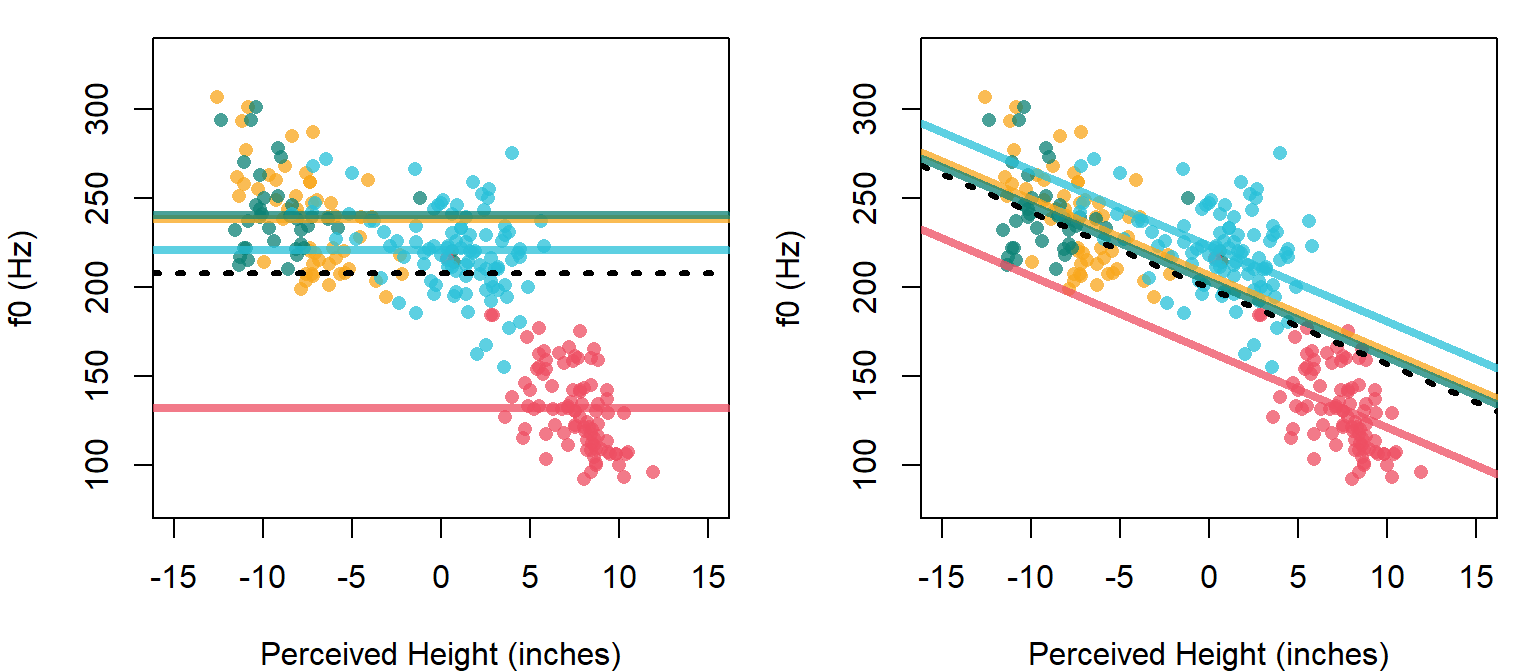
\includegraphics{05_files/figure-latex/F5-55-1.pdf}
\caption{\label{fig:F5-55}(left) Lines for each distribution in our no-slope model. (right) Lines for each distribution in our shared-slope model. Lines correspond to boys (yellow), girls (green), men (red), and women (blue).}
\end{figure}

\hypertarget{interpreting-group-effects-in-the-presence-of-a-continuous-predictor}{%
\subsection{Interpreting group effects in the presence of a continuous predictor}\label{interpreting-group-effects-in-the-presence-of-a-continuous-predictor}}

The inclusion of a continuous predictor affects the interpretation of our group predictors. When we only had a group predictor the group effects had a simple interpretation: they represented the difference between our group mean and the intercept. In terms of our lines however, the group effects actually corresponded to the difference between the line intercept and the overall model intercept. It just so happened that in the previous model our group intercepts corresponded to our group means (because the slopes were 0).

When you include a continuous predictor, the group effects \emph{still} just represent the line intercepts for each group. However, since each line may have a non-zero slope, the group effects will not solely reflect the difference between the group means and the intercept.

Here's a more direct way to think about it: when lines share a slope, group effects affect the spacing between parallel lines. If you look at the right panel of Figure \ref{fig:F5-55} and tilt your head 45 degrees to the right, its clear that the group effects are simply responsible for spacing out the parallel lines. This is the same thing the group effects are doing in the panel on the right.

We're going to compare the estimated group effects provided by the two models presented above (\texttt{group\_intercepts\_model}, and \texttt{group\_single\_slope\_model}). Below, I use the \texttt{hypothesis} function to calculate the group effects according to each model.

\begin{Shaded}
\begin{Highlighting}[]
\NormalTok{group\_intercepts\_effects }\OtherTok{=} 
  \FunctionTok{hypothesis}\NormalTok{ (group\_intercepts\_model,}
              \AttributeTok{hypothesis =} \FunctionTok{c}\NormalTok{(}\StringTok{"group1 = 0"}\NormalTok{, }\CommentTok{\# group 1 effect}
                             \StringTok{"group2 = 0"}\NormalTok{, }\CommentTok{\# group 2 effect}
                             \StringTok{"group3 = 0"}\NormalTok{, }\CommentTok{\# group 3 effect}
                             \StringTok{"{-}(group1+group2+group3) = 0"}\NormalTok{)) }\CommentTok{\# group 4 effect   }
\NormalTok{group\_intercepts\_effects[[}\DecValTok{1}\NormalTok{]][,}\DecValTok{2}\SpecialCharTok{:}\DecValTok{5}\NormalTok{]}
\DocumentationTok{\#\#    Estimate Est.Error   CI.Lower  CI.Upper}
\DocumentationTok{\#\# 1  30.08481  2.896208  24.310787  35.74068}
\DocumentationTok{\#\# 2  32.79653  3.260648  26.583129  39.21910}
\DocumentationTok{\#\# 3 {-}75.75030  2.444318 {-}80.537948 {-}70.93498}
\DocumentationTok{\#\# 4  12.86896  2.358541   8.181246  17.45949}
\end{Highlighting}
\end{Shaded}

\begin{Shaded}
\begin{Highlighting}[]

\NormalTok{group\_single\_slope\_effects }\OtherTok{=} 
  \FunctionTok{hypothesis}\NormalTok{ (group\_single\_slope\_model,}
              \AttributeTok{hypothesis =} \FunctionTok{c}\NormalTok{(}\StringTok{"group1 = 0"}\NormalTok{, }\CommentTok{\# group 1 effect}
                             \StringTok{"group2 = 0"}\NormalTok{, }\CommentTok{\# group 2 effect }
                             \StringTok{"group3 = 0"}\NormalTok{, }\CommentTok{\# group 3 effect}
                             \StringTok{"{-}(group1+group2+group3) = 0"}\NormalTok{) }\CommentTok{\# group 4 effect}
\NormalTok{)   }
\NormalTok{group\_single\_slope\_effects[[}\DecValTok{1}\NormalTok{]][,}\DecValTok{2}\SpecialCharTok{:}\DecValTok{5}\NormalTok{]}
\DocumentationTok{\#\#     Estimate Est.Error    CI.Lower  CI.Upper}
\DocumentationTok{\#\# 1   7.308789  3.820567  {-}0.3534032  14.64993}
\DocumentationTok{\#\# 2   4.204133  4.578811  {-}4.7655678  13.13831}
\DocumentationTok{\#\# 3 {-}35.551710  5.396041 {-}46.0762439 {-}24.96786}
\DocumentationTok{\#\# 4  24.038789  2.546818  19.0232649  29.19051}
\end{Highlighting}
\end{Shaded}

We can use the \texttt{brmplot} function to visually inspect the differences between the group effects across the models. We see that the groups effects are much smaller when the continuous predictor is included. This is visually apparent in the tighter clustering of the lines in the right panel of Figure \ref{fig:F5-int-comparison}. In the absence of group effects we would just see four overlapping lines, one for each group.

\begin{figure}
\centering
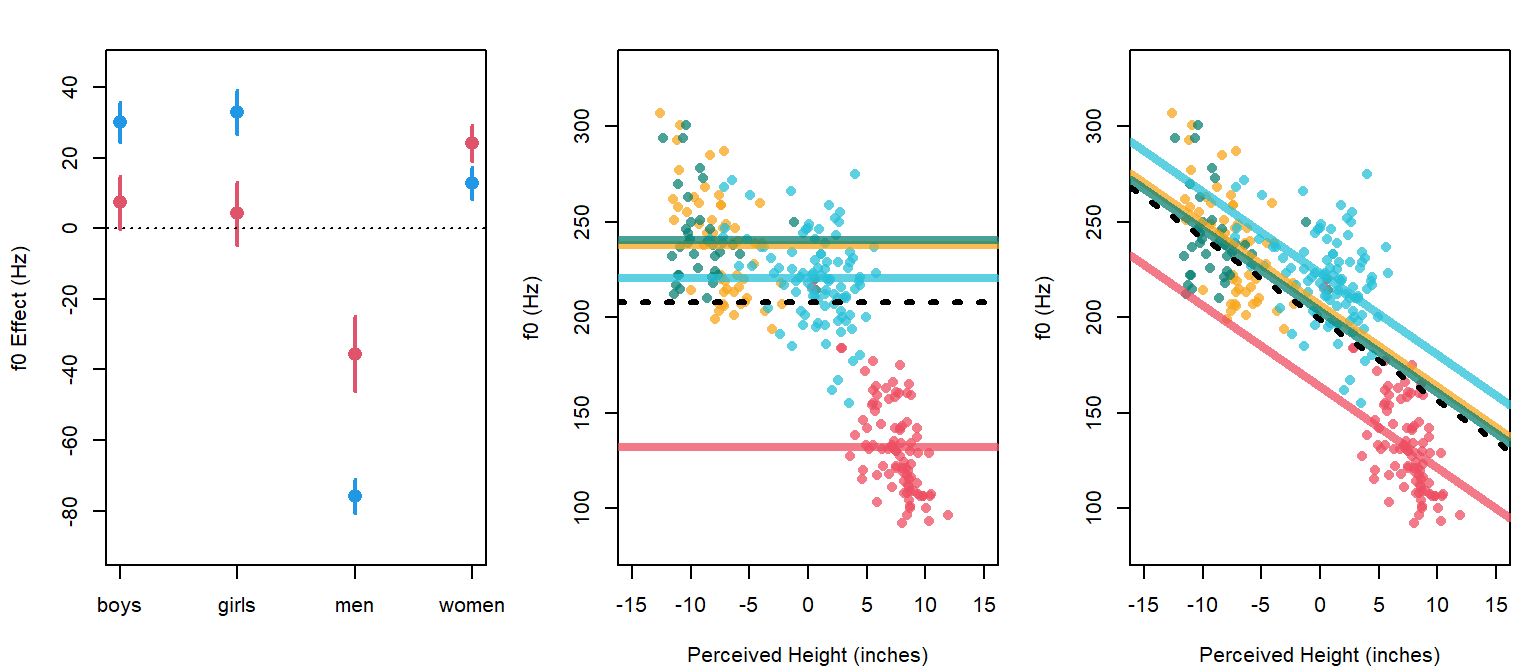
\includegraphics{05_files/figure-latex/F5-int-comparison-1.pdf}
\caption{\label{fig:F5-int-comparison} (left) Comparison of estimated group effects for the model without (blue) and with (red) the perceived height predictor. (middle) Line intercepts reflect the blue coefficients in the left panel (without perceived height). (right) the red coefficients in the left panel (with perceived height). Lines correspond to boys (yellow), girls (green), men (red), and women (blue).}
\end{figure}

So how can we \emph{interpret} the group effects when there is a continuous predictor? The group effects specify the difference in expected values for the dependent variable (\(\mu\), in our case \texttt{f0}) between groups, given \emph{any fixed value of the x axis variable}, in this case perceived height.

To imagine this, pick any arbitrary location along the x-axis in the right panel of Figure \ref{fig:F5-int-comparison}. Then, find the predicted value for f0 for that location by sliding up the y axis until arriving at the black dotted line. The distance along the y axis between the black dotted line (the average line) and the group-specific lines (in different colors) is reflected in the red coefficients in the left panel of Figure \ref{fig:F5-int-comparison}.

Ok, but what do the effects \emph{mean}? The groups effects tell us that \emph{given a certain perceived height}, f0 is lower than expected when the speaker is an adult male, and higher than expected when the speaker is an adult male. In other words, if you think you are listening to a person who is \(x\) inches tall, the most likely f0 associated with that is about 40 Hz lower if the person is a man and about 20 Hz higher if the person is a woman. Importantly, this effect exists \emph{independently} of the relationship between f0 and perceived height.

This is evident in Figure \ref{fig:F5-int-comparison}. The blue line (women) runs parallel to but above the red line (men). Necessarily, for any given x axis location the y axis value will be higher for the blue line than the red line. This is what the group effects are telling us!

Compare this to the effects for girls and boys, which are near zero. When something has an effect near zero this means the `effect' has no effect on outcomes! In this case, we say that for girls and boys, f0 is just about what you would expect given their perceived size. In other words, the perceived-size to f0 relationship for boys and girls is similar to the average relationship. Again, this is evident in Figure \ref{fig:F5-int-comparison} where the green (girls) and yellow (boys) lines overlap with the black dotted line indicating the overall average line.

\hypertarget{models-with-group-dependent-slopes-and-intercepts}{%
\section{Models with group-dependent slopes and intercepts}\label{models-with-group-dependent-slopes-and-intercepts}}

The model above is limited because it is constrained to have the same slope across all the groups. If we want to include different slopes for each group, we must consider the \emph{conditional} effect of perceived height given group. To do this, we need to include the interaction between group and perceived height in our model as in the formula below:

\texttt{f0\ \textasciitilde{}\ group\ *\ pheight}, or \texttt{f0\ \textasciitilde{}\ group\ +\ pheight\ +\ pheight:group}

The model above says: ``model f0 as a function of perceived height, allowing for group-specific variation in the effect for group, and in the effect for perceived height between groups''.

\hypertarget{description-of-the-model-6}{%
\subsection{Description of the model}\label{description-of-the-model-6}}

The `ANOVA-style' decomposition re-introduced with the previous model becomes more useful now. Below we present the `expanded' version of our prediction equation, in a format similar to that presented above. Note that each term that relates to the slope (\(pheight, pheight \colon group\)) is independently multiplied with our predictor (\(x_{[i]}\)).

\[
\mu_{[i]} = Intercept + group_{[\mathrm{group}_{[i]}]} + pheight * x_{[i]} + pheight \colon group_{[\mathrm{group}_{[i]}]} * x_{[i]}
\label{eq:512}
\]

Below, we can group intercept and slope terms in parenthesis. This formulation makes it clear that we expect intercepts and slopes to actually vary trial to trial (whenever the \texttt{group} predictor does).

\begin{equation}
\begin{split}
\mu_{[i]} = (Intercept + group_{[\mathrm{group}_{[i]}]}) + (pheight + pheight \colon group_{[\mathrm{group}_{[i]}]}) * x_{[i]}
\end{split}
\label{eq:513}
\end{equation}

We can take this one step further and break up our prediction equation into two steps. The three equations below say:

\begin{itemize}
\item
  Our expected f0 value varies according to trial-dependent intercept and slope parameters.
\item
  The intercept expected on a given trial is equal to the \(Intercept\) (the intercept main effect) and the \(group\) predictor (effectively, the \(Intercept:group\) interaction).
\item
  The slope expected on a given trial is equal to the \(pheight\) predictor (effectively, the slope `main effect') and the \(pheight:group\) interaction.
\end{itemize}

\begin{equation}
\begin{split}
\mu_{[i]} = a_{[i]} + b_{[i]} * x_{[i]}  \\\\
a_{[i]} = Intercept + group_{[\mathrm{group}_{[i]}]} \\\\
b_{[i]} = pheight + height \colon group_{[\mathrm{group}_{[i]}]}) 
\end{split}
\label{eq:514}
\end{equation}

As our models get more and more complicated, it can help to organize them in this manner. By considering all of our predictors as either `main effects' or `interaction' terms for different predictor variables in our data, we can organize the consideration of how different predictors are expected to relate to outcomes. For example, the representation above makes it clear that the \(height \colon group\) predictor can affect the slopes of our lines, but has no mechanism by which to affect our line intercepts.

We can represent our models in either of the following manners. This representation puts all our predictors directly in the prediction equation:

\begin{equation}
\begin{split}
\textrm{Likelihood:} \\
y_{[i]} \sim \mathcal{N}(\mu_{[i]},\sigma_{error}) \\
\mu_{[i]} = Intercept + group_{[\mathrm{group}_{[i]}]} + pheight * x_{[i]} + pheight \colon group * x_{[i]}  \\ \\
\textrm{Priors:} \\
Intercept \sim t(3, 175, 100) \\
pheight \sim t(3, 0, 100) \\ 
group \sim t(3, 0, 100) \\ 
pheight \colon group \sim t(3, 0, 100) \\ 
\end{split}
\label{eq:515}
\end{equation}

While this representation reflects the decomposition of line intercepts and slopes into several component parts, but is otherwise an identical model:

\begin{equation}
\begin{split}
\textrm{Likelihood:} \\
y_{[i]} \sim \mathcal{N}(\mu_{[i]},\sigma_{error}) \\
\mu_{[i]} = a_{[i]} + b_{[i]} * x_{[i]}  \\ 
a_{[i]} = Intercept + group_{[\mathrm{group}_{[i]}]} \\
b_{[i]} = pheight + height \colon group_{[\mathrm{group}_{[i]}]} \\ \\
\textrm{Priors:} \\
Intercept \sim t(3, 175, 100) \\
pheight \sim t(3, 0, 100) \\ 
group \sim t(3, 0, 100) \\ 
pheight \colon group \sim t(3, 0, 100) \\ 
\end{split}
\label{eq:516}
\end{equation}

\hypertarget{fitting-the-model-5}{%
\subsection{Fitting the model}\label{fitting-the-model-5}}

We fit the model with group-dependent intercepts and slopes below:

\begin{Shaded}
\begin{Highlighting}[]
\CommentTok{\# Fit the model yourself, or}
\CommentTok{\# download pre{-}fit model from: }
\CommentTok{\# github.com/santiagobarreda/stats{-}class/tree/master/models}
\CommentTok{\# and load after placing in working directory}
\CommentTok{\# single\_line\_model = readRDS (\textquotesingle{}5\_group\_multi\_slope\_model.RDS\textquotesingle{})}

\FunctionTok{set.seed}\NormalTok{ (}\DecValTok{1}\NormalTok{)}
\NormalTok{group\_multi\_slope\_model }\OtherTok{=}
  \CommentTok{\#   f0 \textasciitilde{} group * pheight\_c}
  \FunctionTok{brm}\NormalTok{ (f0 }\SpecialCharTok{\textasciitilde{}}\NormalTok{ group }\SpecialCharTok{+}\NormalTok{ pheight\_c }\SpecialCharTok{+}\NormalTok{ pheight\_c}\SpecialCharTok{:}\NormalTok{group, }
       \AttributeTok{data=}\NormalTok{h95, }\AttributeTok{chains=}\DecValTok{1}\NormalTok{,}\AttributeTok{cores=}\DecValTok{1}\NormalTok{,}\AttributeTok{warmup=}\DecValTok{1000}\NormalTok{,}\AttributeTok{iter=}\DecValTok{6000}\NormalTok{,}
       \AttributeTok{prior =} \FunctionTok{c}\NormalTok{(}\FunctionTok{set\_prior}\NormalTok{(}\StringTok{"student\_t(3, 175, 100)"}\NormalTok{, }\AttributeTok{class =} \StringTok{"Intercept"}\NormalTok{),}
                 \FunctionTok{set\_prior}\NormalTok{(}\StringTok{"student\_t(3, 0, 100)"}\NormalTok{, }\AttributeTok{class =} \StringTok{"b"}\NormalTok{)))}
\CommentTok{\# save model}
\CommentTok{\# saveRDS (group\_multi\_slope\_model, \textquotesingle{}5\_group\_multi\_slope\_model.RDS\textquotesingle{})}
\end{Highlighting}
\end{Shaded}

\hypertarget{interpreting-the-model-3}{%
\subsection{Interpreting the model}\label{interpreting-the-model-3}}

We can inspect this model below and see that it contains a relatively large number of parameters. This is a necessary outcome of the complexity of our research question. The model we fit looks for an effect for perceived height on f0, and allows the line relating these variables to vary between groups. Necessarily, this will require the model to present you with 4 intercepts and 4 slopes (or equivalent information), one for each group line.

In fact, if we look below we see that our model has in fact estimated 8 fixed-effect coefficients: 4 slopes and 4 intercepts.

\begin{Shaded}
\begin{Highlighting}[]
\CommentTok{\# inspect model}
\NormalTok{group\_multi\_slope\_model}
\DocumentationTok{\#\#  Family: gaussian }
\DocumentationTok{\#\#   Links: mu = identity; sigma = identity }
\DocumentationTok{\#\# Formula: f0 \textasciitilde{} group + pheight\_c + pheight\_c:group }
\DocumentationTok{\#\#    Data: h95 (Number of observations: 278) }
\DocumentationTok{\#\# Samples: 1 chains, each with iter = 6000; warmup = 1000; thin = 1;}
\DocumentationTok{\#\#          total post{-}warmup samples = 5000}
\DocumentationTok{\#\# }
\DocumentationTok{\#\# Population{-}Level Effects: }
\DocumentationTok{\#\#                  Estimate Est.Error l{-}95\% CI u{-}95\% CI Rhat Bulk\_ESS Tail\_ESS}
\DocumentationTok{\#\# Intercept          204.37      4.39   195.70   213.02 1.00     4426     3198}
\DocumentationTok{\#\# group1             {-}20.32      7.92   {-}35.54    {-}4.94 1.00     2823     3138}
\DocumentationTok{\#\# group2              17.31      8.70     0.15    33.97 1.00     2645     2656}
\DocumentationTok{\#\# group3             {-}14.99      7.44   {-}29.37    {-}0.20 1.00     3081     3243}
\DocumentationTok{\#\# pheight\_c           {-}5.00      0.54    {-}6.07    {-}3.96 1.00     3257     3434}
\DocumentationTok{\#\# group1:pheight\_c    {-}2.33      1.06    {-}4.35    {-}0.25 1.00     2883     3140}
\DocumentationTok{\#\# group2:pheight\_c     2.84      0.98     0.95     4.75 1.00     3112     3394}
\DocumentationTok{\#\# group3:pheight\_c    {-}2.73      1.00    {-}4.71    {-}0.74 1.00     3746     2918}
\DocumentationTok{\#\# }
\DocumentationTok{\#\# Family Specific Parameters: }
\DocumentationTok{\#\#       Estimate Est.Error l{-}95\% CI u{-}95\% CI Rhat Bulk\_ESS Tail\_ESS}
\DocumentationTok{\#\# sigma    21.40      0.92    19.68    23.27 1.00     5004     3185}
\DocumentationTok{\#\# }
\DocumentationTok{\#\# Samples were drawn using sampling(NUTS). For each parameter, Bulk\_ESS}
\DocumentationTok{\#\# and Tail\_ESS are effective sample size measures, and Rhat is the potential}
\DocumentationTok{\#\# scale reduction factor on split chains (at convergence, Rhat = 1).}
\end{Highlighting}
\end{Shaded}

We can recover the overall (main effects) intercept and slope directly from the model estimates. We can get the group-specific intercept and slopes by adding the `main effects' and specific interactions.

\begin{Shaded}
\begin{Highlighting}[]
\NormalTok{group\_multi\_slope\_hypothesis }\OtherTok{=} 
  \FunctionTok{hypothesis}\NormalTok{ (group\_multi\_slope\_model,}
              \AttributeTok{hypothesis =} 
                \FunctionTok{c}\NormalTok{(}\StringTok{"Intercept = 0"}\NormalTok{, }\CommentTok{\# overall intercept}
                  \StringTok{"Intercept + group1 = 0"}\NormalTok{, }\CommentTok{\# group 1 mean}
                  \StringTok{"Intercept + group2 = 0"}\NormalTok{, }\CommentTok{\# group 2 mean}
                  \StringTok{"Intercept + group3 = 0"}\NormalTok{, }\CommentTok{\# group 3 mean}
                  \StringTok{"Intercept + {-}(group1+group2+group3) = 0"}\NormalTok{, }\CommentTok{\# group 4 mean}
                  \StringTok{"pheight\_c = 0"}\NormalTok{, }\CommentTok{\# overall slope}
                  \StringTok{"pheight\_c + group1:pheight\_c = 0"}\NormalTok{, }\CommentTok{\# group 1 slope}
                  \StringTok{"pheight\_c + group2:pheight\_c = 0"}\NormalTok{, }\CommentTok{\# group 2 slope}
                  \StringTok{"pheight\_c + group3:pheight\_c = 0"}\NormalTok{, }\CommentTok{\# group 3 slope}
                  \CommentTok{\# group 4 slope}
                  \StringTok{"pheight\_c +   }
\StringTok{                  {-}(group1:pheight\_c+group2:pheight\_c+group3:pheight\_c) = 0"}\NormalTok{))}
\end{Highlighting}
\end{Shaded}

\begin{Shaded}
\begin{Highlighting}[]
\NormalTok{group\_multi\_slope\_hypothesis[[}\DecValTok{1}\NormalTok{]][,}\DecValTok{2}\SpecialCharTok{:}\DecValTok{5}\NormalTok{]}
\DocumentationTok{\#\#      Estimate  Est.Error   CI.Lower     CI.Upper}
\DocumentationTok{\#\# 1  204.371640  4.3888322 195.700834 213.01668927}
\DocumentationTok{\#\# 2  184.055122  9.6549946 165.203107 203.07234380}
\DocumentationTok{\#\# 3  221.682726 10.7287066 201.014970 242.32745786}
\DocumentationTok{\#\# 4  189.381338  8.8824783 171.980463 207.12968030}
\DocumentationTok{\#\# 5  222.367372  2.2426056 218.070029 226.80771577}
\DocumentationTok{\#\# 6   {-}5.000915  0.5385537  {-}6.067112  {-}3.96349773}
\DocumentationTok{\#\# 7   {-}7.326671  1.2577261  {-}9.761930  {-}4.84173802}
\DocumentationTok{\#\# 8   {-}2.159917  1.1561613  {-}4.406119   0.04965291}
\DocumentationTok{\#\# 9   {-}7.729564  1.1622074 {-}10.011286  {-}5.43739953}
\DocumentationTok{\#\# 10  {-}2.787509  0.6934192  {-}4.168745  {-}1.40028689}
\end{Highlighting}
\end{Shaded}

The first four values above are intercepts, and the next four are slopes. These coefficients are presented in Figure \ref{fig:F5-57}. There appear to be gender-specific patterns in the intercept and slope coefficients between our groups. This pattern is evident when we use the line coefficients to draw each group-dependent line in the panel on the right.

\begin{figure}
\centering
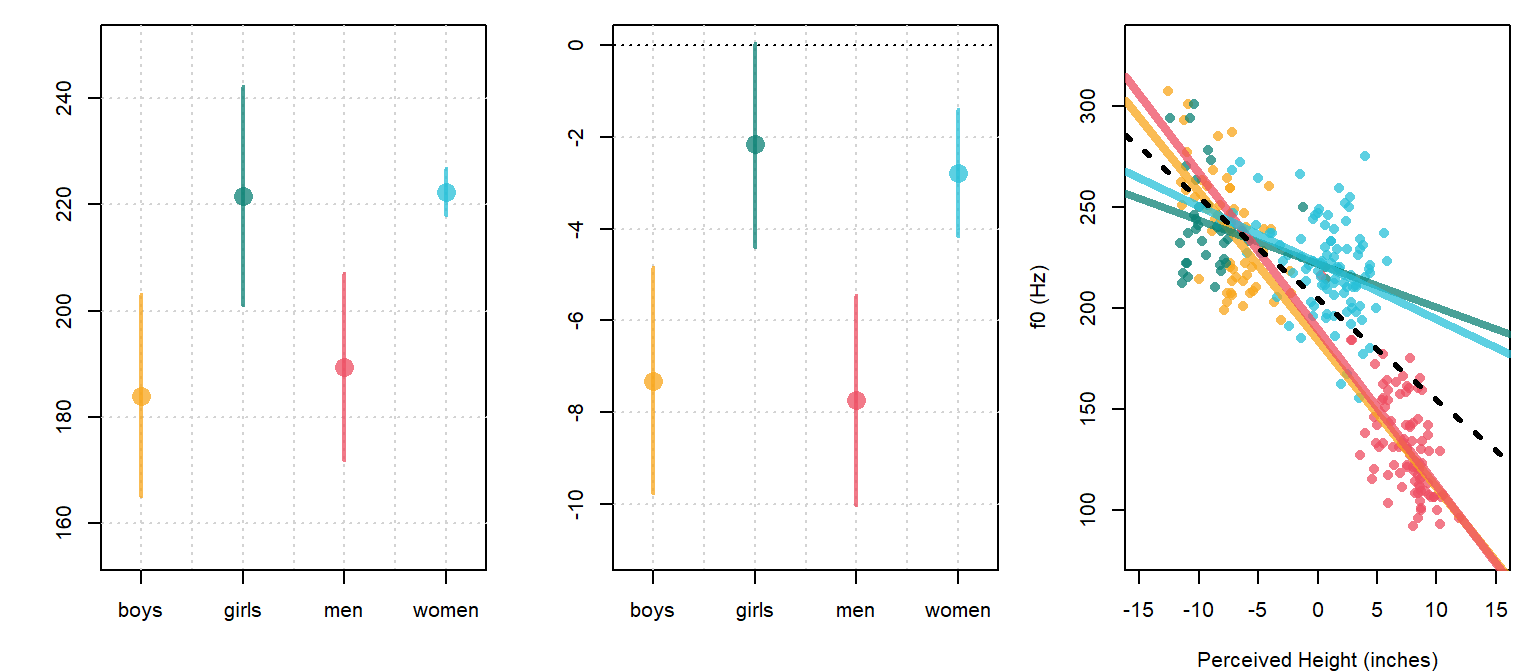
\includegraphics{05_files/figure-latex/F5-57-1.pdf}
\caption{\label{fig:F5-57}(left) Group-specific intercepts. (middle) Group-specific slopes. (right) Lines for each group: boys (yellow), girls (green), men (red), and women (blue).}
\end{figure}

Below, we can see the incremental complexity of the models we have considered and how this complexity requires that our models have more and more coefficients. However, in this case the complexity is justified and reveals group-specific relationships between f0 and perceived height in our data.

\begin{figure}
\centering
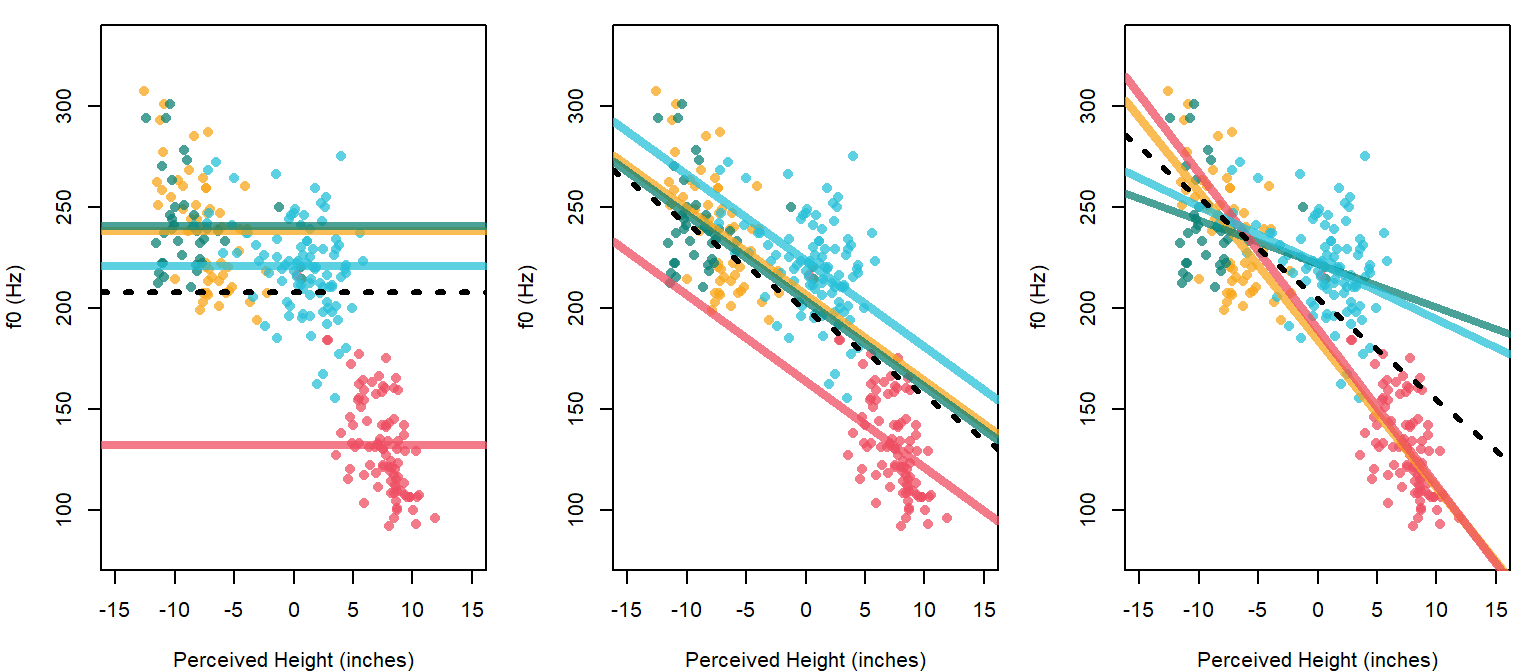
\includegraphics{05_files/figure-latex/F5-group-slopes-1.pdf}
\caption{\label{fig:F5-group-slopes}(left) Group-specific intercepts, slope is zero. (middle) Group-specific intercepts, slope is non-zero but fixed across groups. (right) Group-specific intercepts and group-specific slopes. In each panel, lines correspond to boys (yellow), girls (green), men (red), and women (blue).}
\end{figure}

\hypertarget{exercises-4}{%
\section{Exercises}\label{exercises-4}}

\hypertarget{random-slopes}{%
\chapter{Random slopes}\label{random-slopes}}

To this point we've been fitting realistic, but relatively simple models. In this chapter we're going to build models that are more similar to the sorts that appear in published articles (i.e.~more complicated). Fortunately, we've already discussed all of the component parts that make up our models. We'll see that more complicated models are just made up of many smaller components, all working together.

\hypertarget{data-and-research-questions-5}{%
\section{Data and research questions}\label{data-and-research-questions-5}}

In this chapter we're going to flip the dependent and independent variables from last chapter. We're going to consider variation in perceived height as a function of f0 (and other predictors).

Our data consists of the results of a listening experiment carried out using the Hillenbrand et al.~data. Ten listeners heard productions of `aw' and `iy' produced by all 139 speakers in the dataset. The stimuli consisted of /hVd/ words presented at random (n = 278). For each trial, listeners reported the height of the speaker (in feet and inches) and guessed whether the speaker was a boy, girl, man or woman.

\begin{Shaded}
\begin{Highlighting}[]
\FunctionTok{library}\NormalTok{ (brms)}
\FunctionTok{options}\NormalTok{ (}\AttributeTok{contrasts =} \FunctionTok{c}\NormalTok{(}\StringTok{"contr.sum"}\NormalTok{,}\StringTok{"cont.sum"}\NormalTok{))}

\NormalTok{url1 }\OtherTok{=} \StringTok{"https://raw.githubusercontent.com/santiagobarreda"}
\NormalTok{url2 }\OtherTok{=} \StringTok{"/stats{-}class/master/data/h95\_experiment\_data.csv"}
\NormalTok{h95 }\OtherTok{=} \FunctionTok{read.csv}\NormalTok{ (}\FunctionTok{url}\NormalTok{(}\FunctionTok{paste0}\NormalTok{ (url1, url2)))}
\CommentTok{\# set up colors for plotting}
\NormalTok{devtools}\SpecialCharTok{::}\FunctionTok{source\_url}\NormalTok{ (}\FunctionTok{paste0}\NormalTok{ (url1, }\StringTok{"/stats{-}class/master/data/colors.R"}\NormalTok{))}
\CommentTok{\# source functions}
\NormalTok{devtools}\SpecialCharTok{::}\FunctionTok{source\_url}\NormalTok{ (}\FunctionTok{paste0}\NormalTok{ (url1, }\StringTok{"/stats{-}class/master/data/functions.R"}\NormalTok{))}

\CommentTok{\# calculate centered log f0}
\NormalTok{h95}\SpecialCharTok{$}\NormalTok{g0\_c }\OtherTok{=} \FunctionTok{log}\NormalTok{ (h95}\SpecialCharTok{$}\NormalTok{f0) }\SpecialCharTok{{-}} \FunctionTok{mean}\NormalTok{ (}\FunctionTok{log}\NormalTok{(h95}\SpecialCharTok{$}\NormalTok{f0))}
\end{Highlighting}
\end{Shaded}

We're going to try to understand the role of f0 in size perception because f0 is a very important predictor of apparent talker size. Below we can see the distribution of perceived height plotted according to f0, individually for each subject (i.e.~listener). Clearly, there is a general tendency for perceived height to decrease as f0 increases. This relationship is not really a straight line for most subjects, but is linear enough to try this model as a first step.

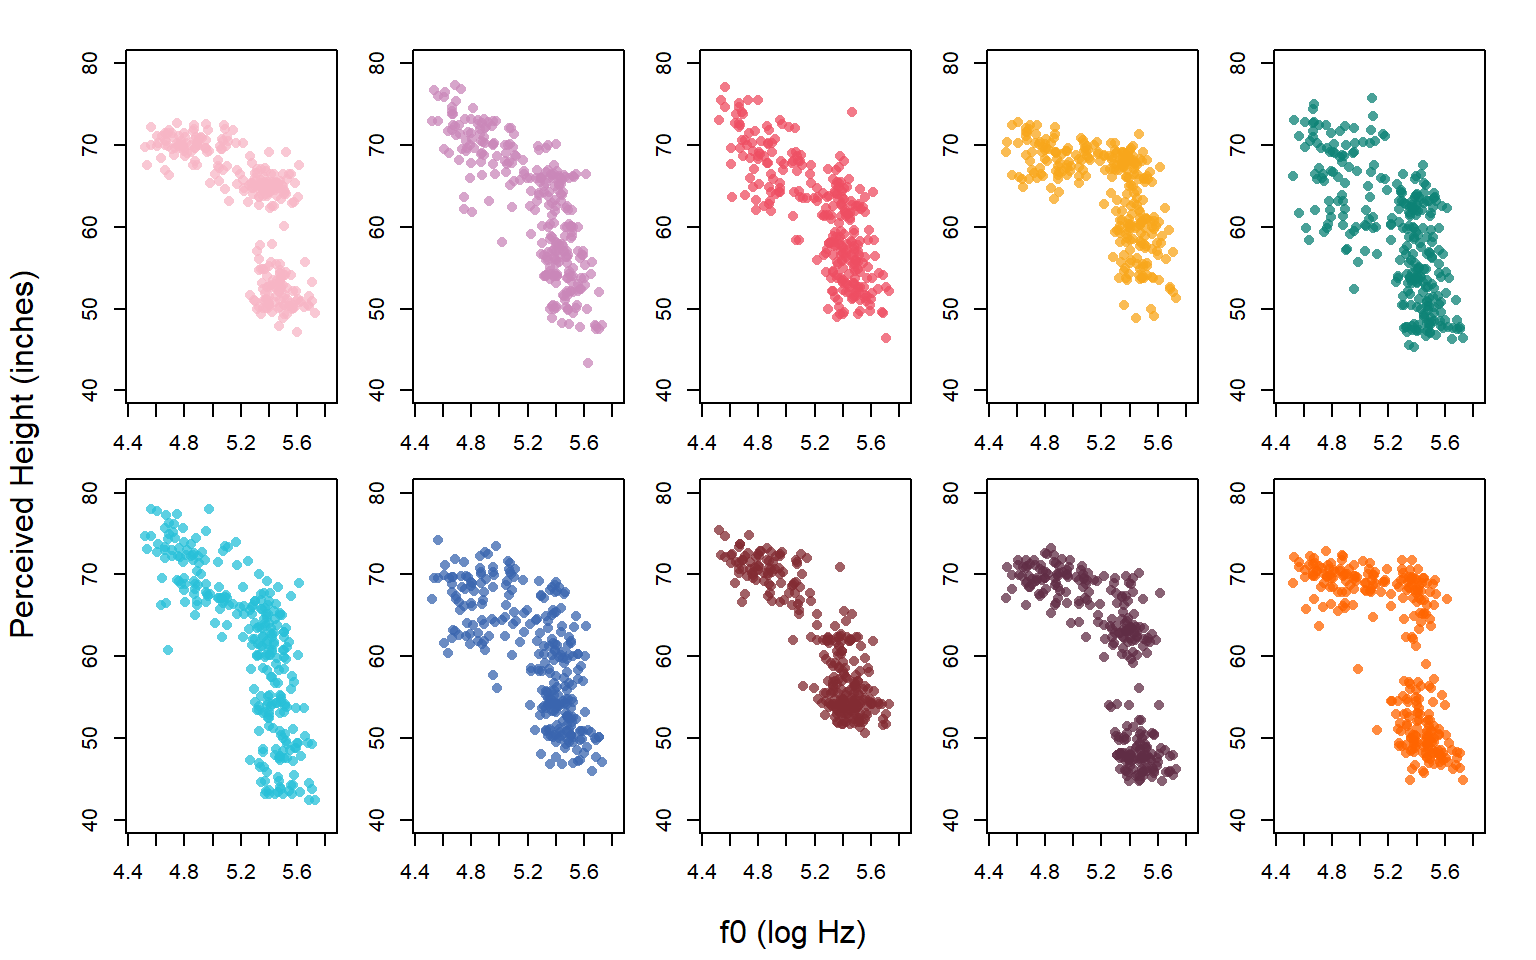
\includegraphics{06_files/figure-latex/F6-1-1.pdf}
In Figure \ref{fig:F6-2}, we compare the data from all subjects using the same colors as above. There is clearly quite a bit of general agreement between listeners. However, we can also clearly see that there is between-subject variation in responses.

\begin{figure}
\centering
\includegraphics{06_files/figure-latex/F6-2-1.pdf}
\caption{\label{fig:F6-2}Distribution of perceived height responses as a function of f0 for all listeners.}
\end{figure}

\hypertarget{repeated-measures-and-speaker-dependent-parameter-values}{%
\section{Repeated measures and speaker-dependent parameter values}\label{repeated-measures-and-speaker-dependent-parameter-values}}

In chapter 5 I mentioned that nominal effects like `group' are effectively interactions with the model intercept for each group, resulting in group-specific intercepts in our model. Interactions between nominal predictors and slope terms (e.g., \(g0\_c \colon group\)) reflect group-specific variation in slopes.

This means that a factor like listener/subject/participant is basically also just an interaction with our intercept representing subject-specific intercepts, and the interactions between subject and our slope term represent subject-specific slopes in our model.

We're going to consider two approaches to including subject-specific slopes and intercepts in our model: one with random slopes by subject, and one with a fixed \(predictor \colon subject\) interaction.

\hypertarget{description-of-the-model-7}{%
\subsection{Description of the model}\label{description-of-the-model-7}}

We're going to predict perceived height (in inches) as a function of centered log-f0 (the logarithm of the fundamental frequency). We're going to let the relationship between f0 and perceived height (related by a line) vary according to subjects. Our model formula is:

\texttt{pheight\ \textasciitilde{}\ g0\_c\ *\ subj\ +\ (1\textbar{}speaker)}

This says ``model perceived height as a function of centered log-f0 (\texttt{g0\_c}) and include subject effects (i.e.~subject-specific intercepts). Also, allow subject-specific use of centered log-f0 in the perception of height (using the g0\_c:subj interaction)''.

We can build this model up from the equation for a single line using the information outlined in the previous chapter. Recall that the formula for a line is:

\[
\mu = a + b * \mathrm{x}
\label{eq:61}
\]

Where our predicted value (\(\mu\)) varies along a line with an intercept of \(a\) and a slope of \(b\). We can decompose the intercept and slope terms in an `ANOVA-like decomposition' as below, given predictors \(A\) and \(B\):

\[
\mu = (Intercept + A + B + ...) + (Slope + Slope \colon A + Slope \colon B + ...) * \mathrm{x}
\label{eq:62}
\]

Above, the line intercept is broken up into a model intercept, and effects for A and B. The slope is broken up into a `main effect' for slope (basically a slope intercept) and the factor by slope interactions (e.g., \(Slope \colon A\)).

Below, the equation is expanded further by removing the parenthesis and multiplying each slope term by our continuous predictor (\(\mathrm{x}\)).

\[
\mu = Intercept + A + B + ... + Slope* \mathrm{x} + slope \colon A* \mathrm{x} + Slope \colon B* \mathrm{x} + ...
\label{eq:63}
\]

As our models get bigger and bigger, expressions like the one above can be difficult to interpret. A presentation like the one below can be clearer and easier to interpret (once you get used to it).

The top line reminds you that you are modeling a line. The second and third lines provide information about expected variation in the intercept and the slope.

\begin{equation}
\begin{split}
\mu = a + b * \mathrm{x} \\
a = Intercept + A + B + ... \\
b = Slope + slope \colon A + Slope \colon B + ... \\
\end{split}
\label{eq:64}
\end{equation}

If you prefer the `expanded' version of the model equation it's easy enough to get this. You simply place all of the components of the \(a\) and \(b\) equations on the same line, and multiply each term in the \(b\) equation by the continuous predictor.

Below is the structure for our model that treats subject as a fixed effect (just like \(group\) in the previous chapter). This model includes subject-specific intercepts for our lines (based on the \(subj\) term) and subject-specific slopes for our lines (based on the \(g0\_c \colon subj\) term). As with our earlier models, this model includes random intercepts for speakers (\(\alpha_{speaker}\)), seen in the intercept equation. Note that our model does \emph{not} include any random effects in the slopes equation.

\begin{equation}
\begin{split}
\textrm{Likelihood:} \\
pheight_{[i]} \sim \mathcal{N}(\mu_{[i]},\sigma_{error}) \\
\mu_{[i]} = a_{[i]} + b_{[i]} * \mathrm{x}_{[i]}  \\ 
a_{[i]} = Intercept + subj_{[\mathrm{subj}_{[i]}]} + \alpha_{[\mathrm{speaker}_{[i]}]}  \\
b_{[i]} =  g0\_c + g0\_c \colon subj_{[\mathrm{subj}_{[i]}]} \\ \\
\textrm{Priors:} \\
\alpha_{speaker} \sim \mathcal{N}(0,\sigma_{speaker}) \\ \\ 
Intercept \sim t(3, 60, 12) \\
g0\_c \sim t(3, 0, 50) \\ 
g0\_c \colon subj \sim t(3, 0, 50) \\ 
subj \sim t(3, 0, 12) \\ 
\sigma_{error} \sim t(3, 0, 12) \\
\sigma_{speaker} \sim t(3, 0, 12) \\ 
\end{split}
\label{eq:65}
\end{equation}

Here's a description of the model in plain English:

\begin{quote}
Perceived height is normally distributed with a mean that varies trial to trial but a fixed standard deviation. The mean (expected value) varies along lines. The lines are specified by intercepts and slopes that vary trom trial to trial, and there is a single continuous predictor (g0\_c). The intercept of these lines vary based on an overall intercept (the main effect), subject-specific deviations from the mean, and speaker-specific deviations from the mean. The slope of these lines vary based on an overall slope (the main effect) and subject-specific deviations from the average slope.
\end{quote}

\begin{quote}
The speaker intercepts were drawn from a normal distribution with a mean of zero and a standard deviation estimated from the data. All other effects (e.g., the Intercept, g0\_c, etc.) were treated as `fixed' and drawn from prior distributions appropriate for their expected range of values (e.g., subj \textasciitilde{} t(3,0,12)).
\end{quote}

\hypertarget{fitting-the-model-6}{%
\subsection{Fitting the model}\label{fitting-the-model-6}}

We fit the model that treats subject as a fixed effect:

\begin{Shaded}
\begin{Highlighting}[]
\CommentTok{\# Fit the model yourself, or}
\CommentTok{\# download pre{-}fit model from: }
\CommentTok{\# github.com/santiagobarreda/stats{-}class/tree/master/models}
\CommentTok{\# and load after placing in working directory}
\CommentTok{\# fixed\_slopes\_model = readRDS (\textquotesingle{}6\_fixed\_slopes\_model.RDS\textquotesingle{})}

\FunctionTok{set.seed}\NormalTok{ (}\DecValTok{1}\NormalTok{)}
\NormalTok{fixed\_slopes\_model }\OtherTok{=}
  \FunctionTok{brm}\NormalTok{ (pheight }\SpecialCharTok{\textasciitilde{}}\NormalTok{ g0\_c }\SpecialCharTok{*}\NormalTok{ subj }\SpecialCharTok{+}\NormalTok{ (}\DecValTok{1}\SpecialCharTok{|}\NormalTok{speaker), }\AttributeTok{data =}\NormalTok{ h95, }\AttributeTok{chains=}\DecValTok{4}\NormalTok{, }\AttributeTok{cores=}\DecValTok{4}\NormalTok{,  }
       \AttributeTok{warmup=}\DecValTok{1000}\NormalTok{, }\AttributeTok{iter =} \DecValTok{7500}\NormalTok{, }\AttributeTok{thin =} \DecValTok{4}\NormalTok{, }\AttributeTok{control =} \FunctionTok{list}\NormalTok{(}\AttributeTok{adapt\_delta =} \FloatTok{0.95}\NormalTok{), }
       \AttributeTok{prior =} \FunctionTok{c}\NormalTok{(}\FunctionTok{set\_prior}\NormalTok{(}\StringTok{"student\_t(3, 60, 12)"}\NormalTok{, }\AttributeTok{class =} \StringTok{"Intercept"}\NormalTok{),}
                 \FunctionTok{set\_prior}\NormalTok{(}\StringTok{"student\_t(3, 0, 50)"}\NormalTok{, }\AttributeTok{class =} \StringTok{"b"}\NormalTok{),}
                 \FunctionTok{set\_prior}\NormalTok{(}\StringTok{"student\_t(3, 0, 12)"}\NormalTok{, }\AttributeTok{class =} \StringTok{"sd"}\NormalTok{)))}

\CommentTok{\# save model}
\CommentTok{\# saveRDS (fixed\_slopes\_model, \textquotesingle{}6\_fixed\_slopes\_model.RDS\textquotesingle{})}
\end{Highlighting}
\end{Shaded}

\hypertarget{interpreting-the-model-4}{%
\subsection{Interpreting the model}\label{interpreting-the-model-4}}

We're going to focus on the model fixed effects. Since we're calculating subject-specific intercepts and slopes, we need 20 coefficients to represents all the lines for our ten subjects. Because we are using sum coding, the \texttt{Intercept} and \texttt{g0\_c} parameters represent our mean overall intercept and slope across all subjects. The \texttt{subj} parameters represent subject-specific deviations from the mean intercept for a given subject, while the \texttt{g0\_c:subject} interactions represent subject specific deviations from the overall slope.

For example, the line representing subject 8's responses can be found by calculating \texttt{Intercept\ +\ subj8} for the intercept and \texttt{g0\_c\ +\ g0\_c:subj8} for the slope.

\begin{Shaded}
\begin{Highlighting}[]
\FunctionTok{fixef}\NormalTok{ (fixed\_slopes\_model)}
\DocumentationTok{\#\#               Estimate Est.Error       Q2.5      Q97.5}
\DocumentationTok{\#\# Intercept  60.98678449 0.4784301 60.0484335 61.9134125}
\DocumentationTok{\#\# g0\_c       {-}6.28597349 1.4033403 {-}8.9682111 {-}3.5214787}
\DocumentationTok{\#\# subj1       1.16432587 0.2191837  0.7370882  1.5905736}
\DocumentationTok{\#\# subj2       1.15897715 0.2178242  0.7268558  1.5884516}
\DocumentationTok{\#\# subj3       0.08484842 0.2191453 {-}0.3439572  0.5161977}
\DocumentationTok{\#\# subj4       3.19209439 0.2196449  2.7737538  3.6216057}
\DocumentationTok{\#\# subj5      {-}1.99350871 0.2183408 {-}2.4207174 {-}1.5651102}
\DocumentationTok{\#\# subj6       0.03808015 0.2185083 {-}0.3916037  0.4690840}
\DocumentationTok{\#\# subj7      {-}1.35476612 0.2171118 {-}1.7884342 {-}0.9376645}
\DocumentationTok{\#\# subj8      {-}0.18965272 0.2172589 {-}0.6200814  0.2400315}
\DocumentationTok{\#\# subj9      {-}1.53045427 0.2166533 {-}1.9543467 {-}1.1057361}
\DocumentationTok{\#\# g0\_c:subj1  0.97782028 0.7314227 {-}0.4547865  2.3773882}
\DocumentationTok{\#\# g0\_c:subj2 {-}1.04728394 0.7340484 {-}2.4842509  0.3662594}
\DocumentationTok{\#\# g0\_c:subj3  1.33942054 0.7252348 {-}0.1290505  2.7669004}
\DocumentationTok{\#\# g0\_c:subj4  7.67663353 0.7400229  6.2212793  9.1142621}
\DocumentationTok{\#\# g0\_c:subj5  2.00732223 0.7318437  0.5799876  3.4735872}
\DocumentationTok{\#\# g0\_c:subj6 {-}4.77805879 0.7323175 {-}6.1988376 {-}3.3397408}
\DocumentationTok{\#\# g0\_c:subj7  2.18304348 0.7355534  0.7304213  3.6183430}
\DocumentationTok{\#\# g0\_c:subj8 {-}2.05792955 0.7389462 {-}3.4984697 {-}0.6021956}
\DocumentationTok{\#\# g0\_c:subj9 {-}4.34455418 0.7365353 {-}5.7989383 {-}2.8925264}
\end{Highlighting}
\end{Shaded}

Since we're treating subject as a factor and using sum coding, we don't get the final level for the subject intercepts or slopes. We can recover this using the hypothesis function, though this can be a bit tedious when there are many levels for a factor.

I wrote a couple of functions that can help with recovering missing factor levels. First, there is a function called \texttt{divide\_factors}. This function takes in a \texttt{brm} model and returns a list of matrices. Each matrix represents the samples for a single main effect or interaction term in your model.

We can apply this function to the model we fit above to inspect the output of the \texttt{divide\_factors} function. Using the \texttt{names} function shows us that our output has four matrices corresponding to the effects for \texttt{(Intercept)},\texttt{g0\_c}, \texttt{subj}, and \texttt{g\_c:subj}.

\begin{Shaded}
\begin{Highlighting}[]
\NormalTok{factors }\OtherTok{=} \FunctionTok{divide\_factors}\NormalTok{ (fixed\_slopes\_model)}
\FunctionTok{names}\NormalTok{ (factors)}
\DocumentationTok{\#\# [1] "(Intercept)" "g0\_c"        "subj"        "g0\_c:subj"}
\end{Highlighting}
\end{Shaded}

We can use the \texttt{str} function to inspect the output. We can see that \texttt{(Intercept)} and \texttt{g0\_c} are vectors of length 6500 (our number of samples), while \texttt{subj} and \texttt{g\_c:subj} are matrices with 6500 rows, but 9 columns (number of subjects - 1).

\begin{Shaded}
\begin{Highlighting}[]
\FunctionTok{str}\NormalTok{ (factors)}
\DocumentationTok{\#\# List of 4}
\DocumentationTok{\#\#  $ (Intercept): num [1:6500] 61.3 61 61.4 60.9 61 ...}
\DocumentationTok{\#\#  $ g0\_c       : num [1:6500] {-}6.31 {-}7.25 {-}7.65 {-}6.45 {-}7.75 ...}
\DocumentationTok{\#\#  $ subj       : num [1:6500, 1:9] 1.017 1.185 1.395 1.298 0.962 ...}
\DocumentationTok{\#\#   ..{-} attr(*, "dimnames")=List of 2}
\DocumentationTok{\#\#   .. ..$ iterations: NULL}
\DocumentationTok{\#\#   .. ..$ parameters: chr [1:9] "subj1" "subj2" "subj3" "subj4" ...}
\DocumentationTok{\#\#  $ g0\_c:subj  : num [1:6500, 1:9] 0.2202 {-}0.0829 0.1943 1.3944 1.5306 ...}
\DocumentationTok{\#\#   ..{-} attr(*, "dimnames")=List of 2}
\DocumentationTok{\#\#   .. ..$ iterations: NULL}
\DocumentationTok{\#\#   .. ..$ parameters: chr [1:9] "g0\_c:subj1" "g0\_c:subj2" "g0\_c:subj3" "g0\_c:subj4" ...}
\end{Highlighting}
\end{Shaded}

We can use a function I wrote called \texttt{add\_missing} which will add missing levels to single factors (it doesn't work for interactions for now). Below, I use this function to recover the missing intercept and slope terms (those of \texttt{subj10}).

\begin{Shaded}
\begin{Highlighting}[]
\NormalTok{factors[[}\StringTok{"subj"}\NormalTok{]] }\OtherTok{=} \FunctionTok{add\_missing}\NormalTok{ (factors[[}\StringTok{"subj"}\NormalTok{]])}
\NormalTok{factors[[}\StringTok{"g0\_c:subj"}\NormalTok{]] }\OtherTok{=} \FunctionTok{add\_missing}\NormalTok{ (factors[[}\StringTok{"g0\_c:subj"}\NormalTok{]])}
\end{Highlighting}
\end{Shaded}

I then use \texttt{brmplot} to plot the speaker intercept and slope effects, including the final recovered set of parameters:

\begin{Shaded}
\begin{Highlighting}[]
\FunctionTok{par}\NormalTok{ (}\AttributeTok{mfrow =} \FunctionTok{c}\NormalTok{(}\DecValTok{1}\NormalTok{,}\DecValTok{2}\NormalTok{), }\AttributeTok{mar =} \FunctionTok{c}\NormalTok{(}\DecValTok{4}\NormalTok{,}\DecValTok{4}\NormalTok{,}\DecValTok{1}\NormalTok{,}\DecValTok{1}\NormalTok{))}
\FunctionTok{brmplot}\NormalTok{ (factors[[}\StringTok{"subj"}\NormalTok{]], }\AttributeTok{col =}\NormalTok{ cols) ; }\FunctionTok{abline}\NormalTok{ (}\AttributeTok{h =} \DecValTok{0}\NormalTok{, }\AttributeTok{lty =} \DecValTok{3}\NormalTok{)}
\FunctionTok{brmplot}\NormalTok{ (factors[[}\StringTok{"g0\_c:subj"}\NormalTok{]], }\AttributeTok{col =}\NormalTok{ cols) ; }\FunctionTok{abline}\NormalTok{ (}\AttributeTok{h =} \DecValTok{0}\NormalTok{, }\AttributeTok{lty =} \DecValTok{3}\NormalTok{)}
\end{Highlighting}
\end{Shaded}

\begin{figure}
\centering
\includegraphics{06_files/figure-latex/f6-3-1.pdf}
\caption{\label{fig:f6-3}(left) Fixed-effects estimates of subject intercept effects. (right) Fixed-effects estimates of subject slope effects.}
\end{figure}

If we want to recover the \emph{actual} speaker-specific intercepts and slopes, we need to add the speaker effects to their corresponding main effects terms. We can do this by adding the column representing each main effect to the matrix representing each set of subject interactions, as below. We could also do this with the hypothesis function but this way we can add all ten subjects' slopes in a single operation, instead of having to write (or even copy) ten lines of code.

\begin{Shaded}
\begin{Highlighting}[]
\NormalTok{subj\_intercepts }\OtherTok{=}\NormalTok{ factors[[}\StringTok{"(Intercept)"}\NormalTok{]] }\SpecialCharTok{+}\NormalTok{ factors[[}\StringTok{"subj"}\NormalTok{]]}
\NormalTok{subj\_slopes }\OtherTok{=}\NormalTok{ factors[[}\StringTok{"g0\_c"}\NormalTok{]] }\SpecialCharTok{+}\NormalTok{ factors[[}\StringTok{"g0\_c:subj"}\NormalTok{]]}
\end{Highlighting}
\end{Shaded}

I want to pause for a moment to highlight that everything to this point has involved the original \textbf{samples} from the posterior, not \emph{summaries} of the samples. Any manipulations done to parameters (including any comparisons) need to be carried out on the samples, and then summarized (never summarized, and then compared).

For example, \texttt{subj\_intercepts}, the sum of the overall intercept and the subject-specific intercept effects is still a matrix with ten columns and 6500 rows, representing the individual samples from the posterior distribution of each parameter.

\begin{Shaded}
\begin{Highlighting}[]
\FunctionTok{head}\NormalTok{( }\FunctionTok{round}\NormalTok{ ( subj\_intercepts , }\DecValTok{3}\NormalTok{ ) )}
\DocumentationTok{\#\#       subj1  subj2  subj3  subj4  subj5  subj6  subj7  subj8  subj9 subj10}
\DocumentationTok{\#\# [1,] 62.339 62.790 61.641 64.905 59.008 61.347 59.750 60.958 59.741 60.750}
\DocumentationTok{\#\# [2,] 62.161 62.134 61.071 64.067 59.011 60.838 59.832 60.910 59.144 60.587}
\DocumentationTok{\#\# [3,] 62.785 62.419 61.316 64.498 59.232 61.654 60.327 61.181 59.824 60.667}
\DocumentationTok{\#\# [4,] 62.180 62.219 60.886 64.023 59.134 60.946 59.616 60.716 58.898 60.195}
\DocumentationTok{\#\# [5,] 61.964 62.323 61.121 64.120 59.261 61.075 59.532 60.542 59.761 60.321}
\DocumentationTok{\#\# [6,] 61.905 61.601 60.894 63.631 58.602 61.029 59.257 60.500 59.197 60.035}
\end{Highlighting}
\end{Shaded}

Only after we are done working with it, we can summarize these matrices:

\begin{Shaded}
\begin{Highlighting}[]
\NormalTok{subj\_intercepts\_summary }\OtherTok{=} \FunctionTok{posterior\_summary}\NormalTok{ (factors[[}\StringTok{"(Intercept)"}\NormalTok{]] }\SpecialCharTok{+}\NormalTok{ factors[[}\StringTok{"subj"}\NormalTok{]])}
\NormalTok{subj\_slopes\_summary }\OtherTok{=} \FunctionTok{posterior\_summary}\NormalTok{ (factors[[}\StringTok{"g0\_c"}\NormalTok{]] }\SpecialCharTok{+}\NormalTok{ factors[[}\StringTok{"g0\_c:subj"}\NormalTok{]])}
\end{Highlighting}
\end{Shaded}

Resulting in a summary of the matrix where each row corresponds to a column from the \texttt{subj\_intercepts} matrix above.

\begin{Shaded}
\begin{Highlighting}[]
\NormalTok{subj\_intercepts\_summary}
\DocumentationTok{\#\#        Estimate Est.Error     Q2.5    Q97.5}
\DocumentationTok{\#\# subj1  62.15111 0.5290596 61.10673 63.16930}
\DocumentationTok{\#\# subj2  62.14576 0.5255985 61.09036 63.15278}
\DocumentationTok{\#\# subj3  61.07163 0.5283570 60.02235 62.10693}
\DocumentationTok{\#\# subj4  64.17888 0.5274135 63.14280 65.19576}
\DocumentationTok{\#\# subj5  58.99328 0.5243383 57.96506 60.01118}
\DocumentationTok{\#\# subj6  61.02486 0.5266767 59.98223 62.03750}
\DocumentationTok{\#\# subj7  59.63202 0.5237791 58.60875 60.64282}
\DocumentationTok{\#\# subj8  60.79713 0.5233061 59.76867 61.81433}
\DocumentationTok{\#\# subj9  59.45633 0.5243279 58.39773 60.45063}
\DocumentationTok{\#\# subj10 60.41684 0.5247678 59.37266 61.42216}
\end{Highlighting}
\end{Shaded}

We can plot the subject effects and the actual subject-specific parameter estimates side by side as in Figure \ref{fig:f6-4}. Clearly, the pattern is the same except for two key differences. First, it is shifted along the y axis due to the addition of the appropriate main effect. Second, the error around the estimates is larger. This is because the estimates on the right represent the sum of the uncertainty in the effect and the uncertainty in the corresponding main effect.

\begin{Shaded}
\begin{Highlighting}[]
\FunctionTok{par}\NormalTok{ (}\AttributeTok{mfrow =} \FunctionTok{c}\NormalTok{(}\DecValTok{2}\NormalTok{,}\DecValTok{2}\NormalTok{), }\AttributeTok{mar =} \FunctionTok{c}\NormalTok{(}\DecValTok{4}\NormalTok{,}\DecValTok{4}\NormalTok{,}\DecValTok{1}\NormalTok{,}\DecValTok{1}\NormalTok{))}
\FunctionTok{brmplot}\NormalTok{ (factors[[}\StringTok{"subj"}\NormalTok{]], }\AttributeTok{col =}\NormalTok{ cols) ; }\FunctionTok{abline}\NormalTok{ (}\AttributeTok{h =} \DecValTok{0}\NormalTok{, }\AttributeTok{lty =} \DecValTok{3}\NormalTok{)}
\FunctionTok{brmplot}\NormalTok{ (subj\_intercepts\_summary, }\AttributeTok{col =}\NormalTok{ cols)}
\FunctionTok{brmplot}\NormalTok{ (factors[[}\StringTok{"g0\_c:subj"}\NormalTok{]], }\AttributeTok{col =}\NormalTok{ cols) ; }\FunctionTok{abline}\NormalTok{ (}\AttributeTok{h =} \DecValTok{0}\NormalTok{, }\AttributeTok{lty =} \DecValTok{3}\NormalTok{)}
\FunctionTok{brmplot}\NormalTok{ (subj\_slopes\_summary, }\AttributeTok{col =}\NormalTok{ cols) ; }\FunctionTok{abline}\NormalTok{ (}\AttributeTok{h =} \DecValTok{0}\NormalTok{, }\AttributeTok{lty =} \DecValTok{3}\NormalTok{)}
\end{Highlighting}
\end{Shaded}

\begin{figure}
\centering
\includegraphics{06_files/figure-latex/f6-4-1.pdf}
\caption{\label{fig:f6-4}(top left) Fixed-effects estimates of subject intercept terms. (top left) Fixed-effects estimates of subject intercept (main effect + subject effect). (bottom left) Fixed-effects estimates of subject slope terms. (bottom right) Fixed-effects estimates of subject slopes (main effect + subject effect).}
\end{figure}

In in Figure \ref{fig:F6-5} we again see the distribution of perceived height plotted according to f0 (centered log-f0), individually for each subject. We can now add lines indicating predicted perceived height based on our model parameters.

\includegraphics{06_files/figure-latex/F6-5-1.pdf}
In Figure in Figure \ref{fig:F6-6}, we again compare the data from all subjects using the same colors as above. This time, we add the regression lines for each subject so that we can compare the similarities/differences between them.

The fit of these models is not great: the predictions they make predictions (the lines) that don't match the data well for \emph{anyone}, suggesting that our model is really missing important information with respect to size perception. However, we're not going to worry about that for now.

\begin{figure}
\centering
\includegraphics{06_files/figure-latex/F6-6-1.pdf}
\caption{\label{fig:F6-6}Distribution of perceived height responses as a function of f0 for all listeners. Lines indicate best-fit lines for each subject.}
\end{figure}

\hypertarget{random-effects-and-the-multivariate-normal-distribution}{%
\section{Random effects and the multivariate normal distribution}\label{random-effects-and-the-multivariate-normal-distribution}}

A model formula like this \texttt{y\ \textasciitilde{}\ 1\ +\ x\ (1\ +\ x\ \textbar{}\ subject)} tells your model to estimate a random intercept for each subject, and also a random effect for \texttt{x} for each speaker. Thus, each level of the clustering factor (\texttt{subject}) is represented by two random parameters, the intercept and the slope for \texttt{x}. Random effects in multilevel models are usually treated as draws from multivariate normal distributions. What I mean by this is that the random intercept and slope for each speaker are treated as a single multidimensional variable, rather than as two independent variables.

The main difference between treating our random coefficients as a single variable rather than two variables is that when we do this, we also estimate the correlation between them. The easiest way to imagine this is by drawing a bivariate (2-dimensional) normal variable and plotting it. This is what I've done below, with simulated intercept and slope parameters drawn at random from a multivariate normal distribution.

In the left column below I compare three bivariate normal variables along the two dimensions. In the absence of any correlation between variables, a plot of this distribution will be \emph{spherical} (or circular in 2 dimensions). When there is a correlation between the two dimensions, the distribution starts looking more and more like a straight line. When there is a negative correlation, the line just points down rather than up.

Note the the marginal (independent) distributions of the variables (the left and right histograms) don't change as the correlation changes. The correlation is a reflection of the \emph{joint} variation in the two variables and will not necessarily be evident in the marginal distributions of each variable.

\begin{figure}
\centering
\includegraphics{06_files/figure-latex/unnamed-chunk-12-1.pdf}
\caption{\label{fig:unnamed-chunk-12}10,000 bivatiate normal draws of simulated intercept and slope coefficients from distributions with a mean of 0 and a standard deviation of 1. The correlation of the variables is 0 (top), 0.5 (middle) and 0.9 (bottom). The left column presents both variables together, the middle column presents intercepts and the right column presents slopes.}
\end{figure}

When our dimensions are uncorrelated they are independent. The value of one does not help you understand the other. However, when the dimensions \emph{are} correlated we can use this to make better predictions using our data. For example, an intercept of 2 in the bottom row in the figure above is very likely to be paired with a slope of 2, but \emph{extremely} unlikely to be seen with a slope of -2. In contrast, in the top row a slope of 2 and -2 seem about equally likely given an intercept of 2. So, when we use multiple random predictors per grouping factor, we are really drawing from a multivariate normal distributions that acknowledges the relationships between random predictors in our data, within-cluster (e.g.~subject/participant/speaker).

The shape of the multivariate normal distribution is determined by a covariance matrix called sigma (\(\Sigma\)). This matrix is a square \(n\) x \(n\) matrix for a variable with \(n\) dimensions. When we dealt with unidimensional normal distributions for our previous random effects, we specified priors for the (unidimensional) standard deviations using t distributions. The specification of priors for our covariance matrix is only slightly more complicated.

In our models, we won't actually include priors for \(\Sigma\) directly. This is because \texttt{brms} (and STAN) build up \(\Sigma\) for us from the components we \emph{do} specify. This is more information that you \emph{really} need, but it helps to understand why the priors are specified the way they are for our random effects.

The covariance matrix for our random effects is created by multiplying the standard deviations of our individual dimensions by a correlation matrix (\(R\)) specifying the correlations between each dimension. The operation is like this:

\begin{equation}
\begin{split}
\Sigma = \begin{bmatrix} \sigma_{\alpha_{[subj]}} & 0 \\ 0 & \sigma_{\beta_{[subj]}} \\ \end{bmatrix} 
\times R \times
\begin{bmatrix} \sigma_{\alpha_{[subj]}} & 0 \\ 0 & \sigma_{\beta_{[subj]}} \\ \end{bmatrix} \\
\end{split}
\label{eq:66}
\end{equation}

The values in the outside matrices are the the standard deviations of the random intercepts (\(\sigma_{\alpha_{[subj]}}\)) and slopes (\(\sigma_{\beta_{[subj]}}\)) individually. The correlation matrix \(R\) contains information about the correlation between the dimensions of the variable (e.g., \(\rho_{\alpha_{[subj]} \beta _{[subj]}}\)).

So, when we have multiple random effects we have a multidimensional variable, and we need to specify priors for each dimension and for the correlation between all dimensions (but not for \(\Sigma\) directly).

We provide priors for the standard deviations of the individual dimensions in the same way as we do for `unidimensional' random effects (like \(\alpha_{[speaker]}\)).

The correlation matrix \(R\) will look something like below (for two dimensions). It will contain only values of 1 on the main diagonal and have mirrored values between -1 and 1 off of the diagonal (since the correlation of a and b equals the correlation of b and a).

\begin{equation}
\begin{split}
R = \begin{bmatrix} x & y \\ y & z \\ \end{bmatrix} \\ \\
\end{split}
\label{eq:67}
\end{equation}

We specify priors for variables of this type using the \(LKJCorr\) distribution in \texttt{brms}. This distribution has a single parameter that determines how peaked the distribution is around 0. Basically, higher numbers make it harder to find larger correlations (and therefore yield more conservative estimates). \href{https://eager-roentgen-523c83.netlify.app/2014/12/27/d-lkj-priors/}{See here for an example}.

\begin{equation}
\begin{split}
R \sim \mathrm{LKJCorr} (2)
\end{split}
\label{eq:672}
\end{equation}

So, any time you have multiple random effects inside any grouping cluster, you need to:

\begin{enumerate}
\def\labelenumi{\arabic{enumi})}
\item
  Specify priors for the standard deviation of each dimension.
\item
  Specify a prior for the correlation matrix for the multivariate normal used for the random parameters.
\end{enumerate}

\hypertarget{random-slopes-1}{%
\section{Random slopes}\label{random-slopes-1}}

The model above was a demonstration that served primarily as a comparison for the model we are going to fit now. No one would actually include subjects as a `fixed' effect, nor would they include the \(g0_c\) by \(subject\) interaction as a fixed effect. In both cases, researchers would tend to include these predictors as `random effects'. Here, we're going to refit the model as a `random slopes' model, and talk about how this is similar/different to our previous approach of treating subjects as fixed effects.

\hypertarget{description-of-the-model-8}{%
\subsection{Description of the model}\label{description-of-the-model-8}}

Our previous model formula was:

\texttt{pheight\ \textasciitilde{}\ g0\_c\ *\ subj\ +\ \ (\ 1\ \textbar{}subj)\ +\ (1\textbar{}speaker)}

This formula allows for subject-specific random intercepts but not slopes. Our new model formula moves \texttt{g0\_c} into the parenthesis with subject like this:

\texttt{pheight\ \textasciitilde{}\ g0\_c\ +\ (\ g0\_c\ \textbar{}subj)\ +\ (1\textbar{}speaker)}

This is the first time we've ever put anything other than \texttt{1} on the left of the pipe in the section where we define random effects. Recall that the factors in parenthesis represent clustering factors. Each of these clusters gets a little mini-model for every level of the factor. So, if subject is our clustering factor, each individual subject (i.e.~each level) gets their own model.

To this point these models have been very simple and have only included intercepts. So, the \texttt{(1\textbar{}speaker)} term says ``we're going to have an intercept for every level of speaker in our model''. In the same way, the \texttt{(\ g0\_c\ \textbar{}subj)} term says ``we're going to have an intercept and a g0\_c slope for every level of subject in our data'' (remember the intercept is assumed even if you don't include a \texttt{1}).

Our model formula could conceivably be written like this (though this won't work because the syntax is wrong):

\texttt{pheight\ \textasciitilde{}\ 1\ +\ g0\_c\ +\ (pheight\ \textasciitilde{}\ 1\ +\ g0\_c\ \textbar{}subj)\ +\ (pheight\ \textasciitilde{}\ 1\textbar{}speaker)}

Again, this won't actually work, but it might be helpful to think of your formulas this way. Notice that the formula inside the subject parenthesis is the same as the formula outside the parenthesis. In each case we are just estimating perceived height according to a slope and an intercept. The equation outside the parentheses (\texttt{pheight\ \textasciitilde{}\ 1\ +\ g0\_c}) tells our model to estimate an overall slope and intercept, and the part inside the parentheses (\texttt{(pheight\ \textasciitilde{}\ 1\ +\ g0\_c\ \textbar{}subj)}) tells our model to do the same thing for each subject. Normally, we omit the \texttt{1} for the intercept, and we only include the dependent variable (and the \texttt{\textasciitilde{}}) in the outside formula. However, the formula above is an accurate representation of what our model formula is really doing.

Ok, so our model has subject specific slopes and intercepts now. You may be thinking ``subject specific intercepts and slopes, isn't that what we did in our last model?''. The answer is yes, it is what we did in our last model! As we'll see below, our `random' and `fixed' effects models are largely the same thing, and provide very similar information. However, there are a few very important differences.

The model description for our random slopes model is given below. The differences relative to our previous model lie in the replacement of our \(subj\) predictor with an \(\alpha_{[\mathrm{subj}]}\) random effect, and the \(g0 \_ c \colon subj\) predictor with a \(\beta_{[\mathrm{subj}]}\) random effect.

\begin{equation}
\begin{split}
\textrm{Likelihood:} \\
y_{[i]} \sim \mathcal{N}(\mu_{[i]},\sigma_{error}) \\
\mu_{[i]} = a_{[i]} + b_{[i]} * \mathrm{x}_{[i]}  \\ 
a_{[i]} = Intercept + \alpha_{[\mathrm{subj}_{[i]}]} + \alpha_{[\mathrm{speaker}_{[i]}]}  \\
b_{[i]} =  g0\_c + \beta_{[\mathrm{subj}_{[i]}]} \\ \\
\textrm{Priors:} \\
\alpha_{speaker} \sim \mathrm{Normal}(0,\sigma_{speaker}) \\ \\  
\begin{bmatrix} \alpha_{subj} \\ \beta_{subj} \end{bmatrix} \sim \mathrm{MVNormal} ( \begin{bmatrix} 0 \\ 0 \\ \end{bmatrix}, \Sigma) \\ \\
Intercept \sim t(3, 60, 12) \\
g0\_c \sim t(3, 0, 50) \\ \\
\sigma_{error} \sim t(3, 0, 100) \\
\sigma_{\alpha_{speaker}} \sim t(3, 0, 100) \\ 
\sigma_{\alpha_{subj}} \sim t(3, 0, 12) \\ 
\sigma_{\beta_{subj}} \sim t(3, 0, 12) \\ 
R \sim \mathrm{LKJCorr} (2)
\end{split}
\label{eq:68}
\end{equation}

Here's a description of the model in plain English:

\begin{quote}
Perceived height is normally distributed with a mean that varies trial to trial but a fixed standard deviation. The mean (expected value) varies along lines. The lines are specified by intercepts and slopes that vary trom trial to trial, and there is a single continuous predictor (g0\_c). The intercept of these lines vary based on an overall intercept (the main effect), subject-specific deviations from the mean, and speaker-specific deviations from the mean. The slope of these lines vary based on an overall slope (the main effect) and subject-specific deviations from the average slope.
\end{quote}

\begin{quote}
The speaker intercepts were drawn from a normal distribution with a mean of zero and a standard deviation estimated from the data. The subject intercepts and slopes were drawn from a bivariate normal distribution with means of 0 of zero and a covariance matrix estimated from the data. All other effects (e.g., the Intercept, g0\_c, etc.) were treated as `fixed' and drawn from prior distributions appropriate for their expected range of values (e.g., subj \textasciitilde{} t(3,0,12)).
\end{quote}

Note that the prediction equation in our last model:

\begin{equation}
\begin{split}
\mu_{[i]} = a_{[i]} + b_{[i]} * \mathrm{x}_{[i]}  \\ 
a_{[i]} = Intercept + subj_{[\mathrm{subj}_{[i]}]} + \alpha_{[\mathrm{speaker}_{[i]}]}  \\
b_{[i]} =  g0\_c + g0\_c \colon subj_{[\mathrm{subj}_{[i]}]} \\ \\
\end{split}
\label{eq:69}
\end{equation}

Is just like the one for this model, save for a one-to-one replacement of the terms \(\alpha_{[\mathrm{subj}]}\) and \(\beta_{[\mathrm{subj}]}\) for \(subj_{[\mathrm{subj}]}\) and \(g0\_c \colon subj_{[\mathrm{subj}]}\):

\begin{equation}
\begin{split}
\mu_{[i]} = a_{[i]} + b_{[i]} * \mathrm{x}_{[i]}  \\ 
a_{[i]} = Intercept + \alpha_{[\mathrm{subj}_{[i]}]} + \alpha_{[\mathrm{speaker}_{[i]}]}  \\
b_{[i]} =  g0\_c + \beta_{[\mathrm{subj}_{[i]}]} \\ \\
\end{split}
\label{eq:610}
\end{equation}

Although the prediction equations are largely the same, in the previous model we treated subject as a `fixed' effect. Remember that in our multilevel Bayesian models, this means that the prior distribution for these was determined entirely a priori and was not estimated from the data. For example our subject effects were drawn from a population of \(subj \sim t(3, 0, 12)\) and the subject by g0\_c interaction was drawn from a population of \(g0\_c \colon subj \sim t(3, 0, 50)\).

In contrast, random effects are drawn from populations whose standard deviation is estimated from the data. This is the way our current (and previous) models treat the speaker effects. Notice that we estimate, rather than stipulate, the standard deviation for the population of speaker effects (\(\sigma_{speaker}\)):

\begin{equation}
\begin{split}
\alpha_{speaker} \sim \mathrm{Normal}(0,\sigma_{speaker}) \\ \\  
\sigma_{speaker} \sim t(3, 0, 100) \\ 
\end{split}
\label{eq:611}
\end{equation}

We might have treated our subject intercepts in the same way, except for the fact that we are also estimating random slopes for subjects. Since we are drawing two random variables for each person, we need to also model the correlation between the variables.

So, when we have multiple random effects (e.g., intercepts and/or slopes) for a predictor, we draw this from a multivariate normal distribution where each predictor is a different `dimension' of the variable. This requires that we estimate a standard deviation for each predictor, and a correlation between each pair of predictors.

As seen below, we draw our predictors from a two-dimensional normal distribution. This distribution has a mean of zero for each dimension, and a covariance matrix equal to \(\Sigma\).

\[
\begin{bmatrix} \alpha_{subj} \\ \beta_{subj} \\ \end{bmatrix}  
\sim \mathrm{MVNormal} ( \begin{bmatrix} 0 \\ 0 \\ \end{bmatrix}, \Sigma) \\ \\
\label{eq:612}
\]

\hypertarget{fitting-the-model-7}{%
\subsection{Fitting the model}\label{fitting-the-model-7}}

We now fit the model that includes random intercepts and by-subject slopes for f0. Notice that my \texttt{set\_prior} section now includes a new category of parameter \texttt{cor} for which I provide a prior using the \texttt{lkj\_corr\_cholesky} distribution.

\begin{Shaded}
\begin{Highlighting}[]
\CommentTok{\# Fit the model yourself, or}
\CommentTok{\# download pre{-}fit model from: }
\CommentTok{\# github.com/santiagobarreda/stats{-}class/tree/master/models}
\CommentTok{\# and load after placing in working directory}
\CommentTok{\# random\_slopes\_model = readRDS (\textquotesingle{}6\_random\_slopes\_model.RDS\textquotesingle{})}

\FunctionTok{set.seed}\NormalTok{ (}\DecValTok{1}\NormalTok{)}
\NormalTok{random\_slopes\_model }\OtherTok{=}
  \FunctionTok{brm}\NormalTok{ (pheight }\SpecialCharTok{\textasciitilde{}}\NormalTok{ g0\_c }\SpecialCharTok{+}\NormalTok{ (g0\_c}\SpecialCharTok{|}\NormalTok{subj) }\SpecialCharTok{+}\NormalTok{ (}\DecValTok{1}\SpecialCharTok{|}\NormalTok{speaker), }\AttributeTok{data=}\NormalTok{h95, }\AttributeTok{chains=}\DecValTok{4}\NormalTok{, }\AttributeTok{cores=}\DecValTok{4}\NormalTok{,  }
       \AttributeTok{warmup=}\DecValTok{1000}\NormalTok{, }\AttributeTok{iter =} \DecValTok{7500}\NormalTok{, }\AttributeTok{thin =} \DecValTok{4}\NormalTok{, }\AttributeTok{control =} \FunctionTok{list}\NormalTok{(}\AttributeTok{adapt\_delta =} \FloatTok{0.95}\NormalTok{), }
       \AttributeTok{prior =} \FunctionTok{c}\NormalTok{(}\FunctionTok{set\_prior}\NormalTok{(}\StringTok{"student\_t(3, 60, 12)"}\NormalTok{, }\AttributeTok{class =} \StringTok{"Intercept"}\NormalTok{),}
                 \FunctionTok{set\_prior}\NormalTok{(}\StringTok{"student\_t(3, 0, 50)"}\NormalTok{, }\AttributeTok{class =} \StringTok{"b"}\NormalTok{),}
                 \FunctionTok{set\_prior}\NormalTok{(}\StringTok{"student\_t(3, 0, 12)"}\NormalTok{, }\AttributeTok{class =} \StringTok{"sd"}\NormalTok{),}
                 \FunctionTok{set\_prior}\NormalTok{(}\StringTok{"lkj\_corr\_cholesky (2)"}\NormalTok{, }\AttributeTok{class =} \StringTok{"cor"}\NormalTok{)))}

\CommentTok{\# save model}
\CommentTok{\# saveRDS (random\_slopes\_model, \textquotesingle{}6\_random\_slopes\_model.RDS\textquotesingle{})}
\end{Highlighting}
\end{Shaded}

\hypertarget{interpreting-the-model-5}{%
\subsection{Interpreting the model}\label{interpreting-the-model-5}}

When we look at the print statement for our model, we now see multiple entries in the \texttt{Group-Level\ Effects} section. Under \texttt{speaker} we see \texttt{sd(Intercept)} representing the standard deviation of the talker intercepts. This tells us that we are only estimating random intercepts for our 139 speakers. These intercepts represent systematic variability in perceived height that is independent of the linear effect for f0.

\begin{verbatim}
Group-Level Effects: 
~speaker (Number of levels: 139) 
              Estimate Est.Error l-95% CI u-95% CI Rhat Bulk_ESS Tail_ESS
sd(Intercept)     5.52      0.47     4.65     6.51 1.00     1643     2982

~subj (Number of levels: 10) 
                    Estimate Est.Error l-95% CI u-95% CI Rhat Bulk_ESS Tail_ESS
sd(Intercept)           1.81      0.54     1.09     3.18 1.00     4776     5714
sd(g0_c)                4.21      1.22     2.54     7.25 1.00     5435     5917
cor(Intercept,g0_c)     0.34      0.27    -0.27     0.77 1.00     5602     5807
\end{verbatim}

We see that there is also a section for \texttt{subj}, containing our by-subject random effects, that has three elements. the first is \texttt{sd(Intercept)}, representing the standard deviation of our subject intercepts. These intercepts represent differences in the average height responses of different subjects that are independent of f0. The second is \texttt{sd(g0\_c)} representing the standard deviation of subject \emph{slopes}. This represents variation in by-subject slopes, analogous to the \(g0_c \colon subj\) interaction in our fixed effects model. The third item is\texttt{cor(Intercept,g0\_c)}, representing the correlation of subject intercepts and subject slopes.

Below, we can compare the fixed effect estimates of our random slopes model:

\begin{verbatim}
Population-Level Effects: 
          Estimate Est.Error l-95% CI u-95% CI Rhat Bulk_ESS Tail_ESS
Intercept    60.93      0.76    59.44    62.43 1.00     1539     3029
g0_c         -6.34      1.94   -10.17    -2.63 1.00     2883     4064
\end{verbatim}

To those of the fixed slopes model.

\begin{verbatim}
Population-Level Effects: 
           Estimate Est.Error l-95% CI u-95% CI Rhat Bulk_ESS Tail_ESS
Intercept     60.99      0.48    60.05    61.91 1.00      713     1735
g0_c          -6.29      1.40    -8.97    -3.52 1.00     1963     3303
\end{verbatim}

The estimates are quite close in value, though their credible intervals vary. The difference in the credible intervals comes across more clearly when we plot them to compare:

\begin{figure}
\centering
\includegraphics{06_files/figure-latex/F6-8-1.pdf}
\caption{\label{fig:F6-8}(left) Comparison of random effect (RE) and fixed effect (FE) estimates of the intercept main effect. (right) Comparison of random effect (RE) and fixed effect (FE) estimates of the slope main effect.}
\end{figure}

We can get the random effects (slopes and intercepts) from our model using the \texttt{ranef} function, and asking for the \texttt{subj} random effects.

\begin{Shaded}
\begin{Highlighting}[]
\NormalTok{random\_effects }\OtherTok{=} \FunctionTok{ranef}\NormalTok{ (random\_slopes\_model)}\SpecialCharTok{$}\NormalTok{subj}
\FunctionTok{str}\NormalTok{ (random\_effects)}
\DocumentationTok{\#\#  num [1:10, 1:4, 1:2] 1.164 1.155 0.116 3.174 {-}1.914 ...}
\DocumentationTok{\#\#  {-} attr(*, "dimnames")=List of 3}
\DocumentationTok{\#\#   ..$ : chr [1:10] "1" "2" "3" "4" ...}
\DocumentationTok{\#\#   ..$ : chr [1:4] "Estimate" "Est.Error" "Q2.5" "Q97.5"}
\DocumentationTok{\#\#   ..$ : chr [1:2] "Intercept" "g0\_c"}
\end{Highlighting}
\end{Shaded}

When we have a look at the output of the \texttt{str} function, we can see that this is a 3-dimensional matrix. When we look at this matrix along the third dimension (e.g., \texttt{random\_effects{[},,in\ here{]}}), we get a series of 2-d matrices that are a summary of a single random effect. Below we see that the first matrix (\texttt{random\_effects{[},,1{]}}) corresponds to the random intercepts, and the second matrix (\texttt{random\_effects{[},,2{]}}) corresponding to the random slopes.

You'll note that we actually get all ten subject effects and there is no omitted value. This is because when you use partial pooling to estimate parameters, you actually \emph{can} estimate all levels of a factor (for technical reasons related to shrinkage).

\begin{Shaded}
\begin{Highlighting}[]
\NormalTok{random\_effects}
\DocumentationTok{\#\# , , Intercept}
\DocumentationTok{\#\# }
\DocumentationTok{\#\#       Estimate Est.Error        Q2.5       Q97.5}
\DocumentationTok{\#\# 1   1.16377527 0.6268821 {-}0.04942324  2.46153571}
\DocumentationTok{\#\# 2   1.15505273 0.6275566 {-}0.03510937  2.42001233}
\DocumentationTok{\#\# 3   0.11623493 0.6231278 {-}1.10121480  1.38309357}
\DocumentationTok{\#\# 4   3.17445575 0.6258360  1.99622247  4.49472090}
\DocumentationTok{\#\# 5  {-}1.91413822 0.6259466 {-}3.12790488 {-}0.63922912}
\DocumentationTok{\#\# 6   0.04515396 0.6257749 {-}1.18640204  1.32431108}
\DocumentationTok{\#\# 7  {-}1.28080815 0.6267446 {-}2.50106938 {-}0.03644058}
\DocumentationTok{\#\# 8  {-}0.16633822 0.6317497 {-}1.39801195  1.11656287}
\DocumentationTok{\#\# 9  {-}1.47968132 0.6320220 {-}2.71728703 {-}0.21591965}
\DocumentationTok{\#\# 10 {-}0.53282781 0.6300846 {-}1.74720063  0.75334092}
\DocumentationTok{\#\# }
\DocumentationTok{\#\# , , g0\_c}
\DocumentationTok{\#\# }
\DocumentationTok{\#\#      Estimate Est.Error      Q2.5     Q97.5}
\DocumentationTok{\#\# 1   1.0157799  1.577586 {-}2.117585  4.117939}
\DocumentationTok{\#\# 2  {-}0.9027227  1.566411 {-}4.070686  2.179692}
\DocumentationTok{\#\# 3   1.3279988  1.577451 {-}1.798952  4.516177}
\DocumentationTok{\#\# 4   7.4737121  1.591885  4.444100 10.670002}
\DocumentationTok{\#\# 5   1.8695128  1.569712 {-}1.300681  5.008267}
\DocumentationTok{\#\# 6  {-}4.4944108  1.569323 {-}7.674207 {-}1.418619}
\DocumentationTok{\#\# 7   2.0829323  1.582772 {-}1.030887  5.365565}
\DocumentationTok{\#\# 8  {-}1.9113901  1.578336 {-}5.155632  1.199296}
\DocumentationTok{\#\# 9  {-}4.1408383  1.578127 {-}7.315184 {-}1.035547}
\DocumentationTok{\#\# 10 {-}1.8307910  1.561144 {-}4.991040  1.268622}
\end{Highlighting}
\end{Shaded}

In Figure \ref{fig:p6-10}, we see a comparison of the subject intercept and slope terms provided by the random and fixed slopes models. We can see that the effects are extremely similar, however, credible intervals are substantially wider for the estimates provided by the random effects model.

\begin{Shaded}
\begin{Highlighting}[]
\FunctionTok{par}\NormalTok{ (}\AttributeTok{mfrow =} \FunctionTok{c}\NormalTok{(}\DecValTok{2}\NormalTok{,}\DecValTok{1}\NormalTok{), }\AttributeTok{mar =} \FunctionTok{c}\NormalTok{(}\DecValTok{4}\NormalTok{,}\DecValTok{4}\NormalTok{,}\DecValTok{1}\NormalTok{,}\DecValTok{1}\NormalTok{))}
\CommentTok{\# plot random intercepts}
\FunctionTok{brmplot}\NormalTok{ (}\AttributeTok{xs =}\NormalTok{ (}\DecValTok{1}\SpecialCharTok{:}\DecValTok{10}\NormalTok{)}\SpecialCharTok{{-}}\NormalTok{.}\DecValTok{2}\NormalTok{,  random\_effects[,,}\DecValTok{1}\NormalTok{], }\AttributeTok{col=}\NormalTok{cols, }\AttributeTok{labels =} \StringTok{""}\NormalTok{, }\AttributeTok{pch=}\DecValTok{15}\NormalTok{)}
\CommentTok{\# plot fixed intercepts}
\FunctionTok{brmplot}\NormalTok{ (}\AttributeTok{xs =}\NormalTok{ (}\DecValTok{1}\SpecialCharTok{:}\DecValTok{10}\NormalTok{)}\SpecialCharTok{+}\NormalTok{.}\DecValTok{2}\NormalTok{, factors[[}\StringTok{"subj"}\NormalTok{]], }\AttributeTok{add =} \ConstantTok{TRUE}\NormalTok{, }\AttributeTok{col=}\NormalTok{cols)}
\FunctionTok{abline}\NormalTok{ (}\AttributeTok{h=}\DecValTok{0}\NormalTok{, }\AttributeTok{lty=}\DecValTok{3}\NormalTok{)}
\CommentTok{\# plot random slopes}
\FunctionTok{brmplot}\NormalTok{ (}\AttributeTok{xs =}\NormalTok{ (}\DecValTok{1}\SpecialCharTok{:}\DecValTok{10}\NormalTok{)}\SpecialCharTok{{-}}\NormalTok{.}\DecValTok{2}\NormalTok{, random\_effects[,,}\DecValTok{2}\NormalTok{], }\AttributeTok{col =}\NormalTok{ cols, }\AttributeTok{labels =} \StringTok{""}\NormalTok{, }\AttributeTok{pch=}\DecValTok{15}\NormalTok{)}
\CommentTok{\# plot fixed slopes}
\FunctionTok{brmplot}\NormalTok{ (}\AttributeTok{xs =}\NormalTok{ (}\DecValTok{1}\SpecialCharTok{:}\DecValTok{10}\NormalTok{)}\SpecialCharTok{+}\NormalTok{.}\DecValTok{2}\NormalTok{, factors[[}\StringTok{"g0\_c:subj"}\NormalTok{]], }\AttributeTok{add =} \ConstantTok{TRUE}\NormalTok{, }\AttributeTok{col=}\NormalTok{cols)}
\FunctionTok{abline}\NormalTok{ (}\AttributeTok{h=}\DecValTok{0}\NormalTok{, }\AttributeTok{lty=}\DecValTok{3}\NormalTok{)}
\end{Highlighting}
\end{Shaded}

\begin{figure}
\centering
\includegraphics{06_files/figure-latex/p6-10-1.pdf}
\caption{\label{fig:p6-10}(top) Comparison of random effects (squares) and fixed effect (circles) estimates for speaker intercept effects. (bottom) Same as above but for the slope terms.}
\end{figure}

In Figure \ref{fig:F6-10}, we compare the random and fixed effects estimates for the subject intercepts. Note that the difference between the random and fixed effect estimates is largest for the effects with the largest magnitude. For example, on the left edge of the right figure below we see that the green effect with a fixed effect estimates near -2 has a random effect that is nearly 0.1 larger than that (near to -1.9).

\begin{figure}
\centering
\includegraphics{06_files/figure-latex/F6-10-1.pdf}
\caption{\label{fig:F6-10}(left) Comparison of fixed and random estimates for subject effects (intercept terms). (right) Plot of the difference between the estimates for each parameter, plotted against the value of the fixed-effect estimate of the same parameter.}
\end{figure}

The same pattern is evident in Figure \ref{fig:F6-11}, : more extreme values are `shrunk' towards the mean. This is partial-pooling and shrinkage in action! Because parameters in a `random effect' are jointly estimated (to some extent), extreme values can be pulled towards the mean when they are weakly supported. Here we see a tiny bit of shrinkage indicating that: 1) the values were not so extreme, and 2) the `extreme' values had a reasonable amount of support.

\begin{figure}
\centering
\includegraphics{06_files/figure-latex/F6-11-1.pdf}
\caption{\label{fig:F6-11}(left) Comparison of fixed and random estimates for g0\_c:subject effects (slope terms). (right) Plot of the difference between the estimates for each parameter, plotted against the value of the fixed-effect estimate of the same parameter.}
\end{figure}

\hypertarget{more-predictors-and-more-random-slopes}{%
\section{More predictors and more random slopes}\label{more-predictors-and-more-random-slopes}}

\hypertarget{adding-another-random-slope}{%
\subsection{Adding another random slope}\label{adding-another-random-slope}}

Imagine we were to add another continuous predictor to our model. We can use the centered logarithm of F1 (\texttt{g1\_c}) as an example. Inclusion of random slopes for this predictor would mean our equation now looks like:

\texttt{pheight\ \textasciitilde{}\ g0\_c\ +\ g1\_c\ (g0\_c\ +\ g1\_c\textbar{}subj)\ +\ (1\textbar{}speaker)}

In turn, this means that the likelihood section of our model now looks like below. Basically, we have just added a new continuous predictor (\(\mathrm{x}_{2[i]}\)) and slope term (\(b_{2}\)), with its own corresponding decomposition into a main effect and a random subject effect.

\begin{equation}
\begin{split}
y_{[i]} \sim \mathcal{N}(\mu_{[i]},\sigma_{error}) \\
\mu_{[i]} = a_{[i]} + b_{1[i]} * \mathrm{x}_{1[i]} + b_{2[i]} * \mathrm{x}_{2[i]}  \\ 
a_{[i]} = Intercept + \alpha_{[\mathrm{subj}_{[i]}]} + \alpha_{[\mathrm{speaker}_{[i]}]}  \\
b_{1[i]} =  g0\_c + \beta_{1{[\mathrm{subj}_{[i]}]}} \\ 
b_{2[i]} =  g1\_c + \beta_{2{[\mathrm{subj}_{[i]}]}} \\ 
\end{split}
\label{eq:613}
\end{equation}

The two random slopes (\(\beta_{1{[\mathrm{subj}]}},\beta_{2{[\mathrm{subj}]}}\)) and the random intercept (\(\alpha_{[\mathrm{subj}]}\)) are all drawn from a multivariate normal distribution:

\begin{equation}
\begin{split}
\begin{bmatrix} \alpha_{[subj]} \\ \beta_{1[subj]} \\ \beta_{2[subj]} \\ \end{bmatrix}  
\sim \mathrm{MVNormal} ( \begin{bmatrix} 0 \\ 0 \\ 0 \\ \end{bmatrix}, \Sigma) \\ 
\end{split}
\label{eq:613}
\end{equation}

Just as for our first random slopes model, we just need to worry about specifying the priors for the effects standard deviations (\(\sigma_{\alpha_{[\mathrm{speaker}]}}, \sigma_{\beta_{[\mathrm{speaker}]}}\)) and the correlation matrix (\(R\)) (like below) and \texttt{brm} does the rest of the work for us.

\begin{equation}
\begin{split}
\sigma_{\alpha_{[speaker]}} \sim t(3, 0, 100) \\ 
\sigma_{\beta_{1[subj]}} \sim t(3, 0, 100) \\ 
\sigma_{\beta_{2[subj]}} \sim t(3, 0, 100) \\ 
R \sim \mathrm{LKJCorr} (2)
\end{split}
\label{eq:614}
\end{equation}

\hypertarget{adding-random-factors}{%
\subsection{Adding random factors}\label{adding-random-factors}}

We can also add random effects for factors. For example, we could include \texttt{adult} inside our \texttt{subj} parentheses in the model formula. This would tell our model to calculate a subject-specific effect for \texttt{adult}:

\texttt{pheight\ \textasciitilde{}\ g0\_c\ +\ g1\_c\ +\ adult\ (g0\_c\ +\ g1\_c\ +\ adult\ \textbar{}subj)\ +\ (1\textbar{}speaker)}

The likelihood section of our model will now look like below. Note that the random effect associated with adultness is added to the intercept equation. This is because this effect does not interact with our continuous predictors. Since there are no interactions between our continuous predictors and the adult effect, the slopes cannot vary based on adultness. As a result, the adultness parameter can only affect the intercepts of the shapes being drawn and not the slopes.

\begin{equation}
\begin{split}
y_{[i]} \sim \mathcal{N}(\mu_{[i]},\sigma_{error}) \\
\mu_{[i]} = a_{[i]} + b_{1[i]} * \mathrm{x}_{1[i]} + b_{2[i]} * \mathrm{x}_{2[i]}  \\ 
a_{[i]} = Intercept + \alpha_{[\mathrm{subj}_{[i]}]} + \alpha_{adult[\mathrm{subj}_{[i]}]} + \alpha_{[\mathrm{speaker}_{[i]}]}  \\
b_{1[i]} =  g0\_c + \beta_{1{[\mathrm{subj}_{[i]}]}} \\ 
b_{2[i]} =  g1\_c + \beta_{2{[\mathrm{subj}_{[i]}]}} \\ \\
\end{split}
\label{eq:614}
\end{equation}

Since we now have 4 random effects for subject, we draw our subject random effects from a four-dimensional normal distribution like this:

\begin{equation}
\begin{split}
\begin{bmatrix} \alpha_{[subj]} \\ \alpha_{adult[subj]} \\ \beta_{1[subj]} \\ \beta_{2[subj]} \\ \end{bmatrix}  
\sim \mathrm{MVNormal} ( \begin{bmatrix} 0 \\ 0 \\ 0 \\ 0 \\ \end{bmatrix}, \Sigma) \\ \\
\end{split}
\label{eq:615}
\end{equation}

\hypertarget{the-independence-of-continuous-predictors}{%
\subsection{The independence of continuous predictors}\label{the-independence-of-continuous-predictors}}

It's important to note that each continuous predictor is treated independently in our model. We could, for example, include an interaction between adultness and F1 in our model. This would make the formula look like this:

\texttt{pheight\ \textasciitilde{}\ g0\_c\ +\ g1\_c\ +\ adult\ +\ g1\_c:adult\ +\ (g0\_c\ +\ g1\_c\ +\ adult\ +\ g1\_c:adult\textbar{}subj)\ +\ (1\textbar{}speaker)}

Note that this only causes a change for one of our slopes (\(b_2\)). It causes no change at all for our intercept or the other slope:

\begin{equation}
\begin{split}
y_{[i]} \sim \mathcal{N}(\mu_{[i]},\sigma_{error}) \\
\mu_{[i]} = a_{[i]} + b_{1[i]} * \mathrm{x}_{1[i]} + b_{2[i]} * \mathrm{x}_{2[i]}  \\ 
a_{[i]} = Intercept + \alpha_{[\mathrm{subj}_{[i]}]} + \alpha_{adult[\mathrm{subj}_{[i]}]} + \alpha_{[\mathrm{speaker}_{[i]}]}  \\
b_{1[i]} =  g0\_c + \beta_{1{[\mathrm{subj}_{[i]}]}} \\ 
b_{2[i]} =  g1\_c + \beta_{2{[\mathrm{subj}_{[i]}]}} + \beta_{2,adult[\mathrm{subj}_{[i]}]} \\ 
\end{split}
\label{eq:616}
\end{equation}

Since we now have five random effects, we now draw our subject random effects from a five-dimensional normal distribution like:

\begin{equation}
\begin{split}
\begin{bmatrix} \alpha_{[subj]} \\ \alpha_{adult[subj]} \\ \beta_{1[subj]} \\ \beta_{2[subj]} \\ \beta_{2,adult[\mathrm{subj}_{[i]}]} \\ \end{bmatrix}  
\sim \mathrm{MVNormal} ( \begin{bmatrix} 0 \\ 0 \\ 0 \\ 0 \\ 0 \\ \end{bmatrix}, \Sigma) \\ \\
\end{split}
\label{eq:616}
\end{equation}

Keep in mind that the correlation matrix for this distribution is a 5x5 matrix with 25 elements, meaning we have to estimate 10 correlation parameters and 5 variance parameters in order to estimate these random effects. Many of the convergence problems that \texttt{lmer} has seem to relate to the estimation of the correlation parameters for random slopes. Since our Bayesian models have prior distributions on these correlation parameters, they can do a much better job of investigating the random effects correlations and can therefore easily (but perhaps slowly) find solutions for models with even large numbers of random effects.

\hypertarget{answering-our-research-questions-1}{%
\section{Answering our research questions}\label{answering-our-research-questions-1}}

Let's look at the output of our random slopes model again to see where we stand with respect to our research question:

\begin{verbatim}
##  Family: gaussian 
##   Links: mu = identity; sigma = identity 
## Formula: pheight ~ g0_c + (g0_c | subj) + (1 | speaker) 
##    Data: h95 (Number of observations: 2780) 
## Samples: 4 chains, each with iter = 7500; warmup = 1000; thin = 4;
##          total post-warmup samples = 6500
## 
## Group-Level Effects: 
## ~speaker (Number of levels: 139) 
##               Estimate Est.Error l-95% CI u-95% CI Rhat Bulk_ESS Tail_ESS
## sd(Intercept)     5.52      0.47     4.65     6.51 1.00     1643     2982
## 
## ~subj (Number of levels: 10) 
##                     Estimate Est.Error l-95% CI u-95% CI Rhat Bulk_ESS Tail_ESS
## sd(Intercept)           1.81      0.54     1.09     3.18 1.00     4776     5714
## sd(g0_c)                4.21      1.22     2.54     7.25 1.00     5435     5917
## cor(Intercept,g0_c)     0.34      0.27    -0.27     0.77 1.00     5602     5807
## 
## Population-Level Effects: 
##           Estimate Est.Error l-95% CI u-95% CI Rhat Bulk_ESS Tail_ESS
## Intercept    60.93      0.76    59.44    62.43 1.00     1539     3029
## g0_c         -6.34      1.94   -10.17    -2.63 1.00     2883     4064
## 
## Family Specific Parameters: 
##       Estimate Est.Error l-95% CI u-95% CI Rhat Bulk_ESS Tail_ESS
## sigma     3.83      0.05     3.73     3.94 1.00     5831     6083
## 
## Samples were drawn using sampling(NUTS). For each parameter, Bulk_ESS
## and Tail_ESS are effective sample size measures, and Rhat is the potential
## scale reduction factor on split chains (at convergence, Rhat = 1).
\end{verbatim}

There is clearly an effect for f0 on perceived height. If we were so inclined we could leave it at that. However, we can do a very simple form of posterior prediction by considering the lines generated by our models. In the figure below (recreated from above) we can see that the lines are actually doing a pretty terrible job of predicting where the data is. In most cases, there is no data where the line actually is!

\begin{figure}
\centering
\includegraphics{06_files/figure-latex/F6-12-1.pdf}
\caption{\label{fig:F6-12}Each plot shows responses from a single subject. Lines indicate best fit line relating variables, as indicated by our fixed slopes model.}
\end{figure}

When we look at the model statement above, we can see that the residual error (\texttt{sigma}, \(\sigma_{error}\)) is only 3.8 inches, meaning our model can predict perceived height with an expected error of 3.8 inches. That doesn't seem that bad. However, if we look at the standard deviation for the speaker intercepts (\texttt{sd(Intercept)} under \texttt{\textasciitilde{}speaker}, \(\sigma_{\alpha_{[speaker]}}\)) we can see that this is 5.5 inches. In other words, our model contains large amounts of speaker specific variation in perceived height. This variation is `explained' by the random effects in our model, but is not being explained by f0. We can inspect these below:

\begin{figure}
\centering
\includegraphics{06_files/figure-latex/F6-13-1.pdf}
\caption{\label{fig:F6-13}Speaker random intercepts and credible intervals colored by group (red = boys, yellow = girls, green = men, blue = women).}
\end{figure}

Remember, these `random' effects are being modeled as being normally distributed with a mean of 0. The distribution of random effects clearly shows a systematic pattern according to speaker group. In general, boys and girls are perceived as smaller than expected given their f0, men are perceived as taller than expected given their f0, and women are perceived as being about as tall as expected given their f0.

The speaker intercepts above show a remarkable amount of consistency within group. Keep in mind that listeners were not told the group the speaker belonged to, so either 1) listener guessed speaker group and used this to guess size, or 2) there are other acoustic cues that vary systematically between groups, and listeners used this to estimate size. In either case, this suggests that our model need to change in order to really capture how listeners are arriving at size judgments for these speakers.

\hypertarget{lmer-corner-2}{%
\section{Lmer corner}\label{lmer-corner-2}}

We can fit a `random slopes' model with \texttt{lmer} using the code below:

\begin{Shaded}
\begin{Highlighting}[]
\NormalTok{model }\OtherTok{=}\NormalTok{ lme4}\SpecialCharTok{::}\FunctionTok{lmer}\NormalTok{ (pheight }\SpecialCharTok{\textasciitilde{}}\NormalTok{ g0\_c }\SpecialCharTok{+}\NormalTok{  (g0\_c}\SpecialCharTok{|}\NormalTok{subj) }\SpecialCharTok{+}\NormalTok{ (}\DecValTok{1}\SpecialCharTok{|}\NormalTok{speaker), }\AttributeTok{data =}\NormalTok{ h95)}
\end{Highlighting}
\end{Shaded}

Below I recreate the middle part of the \texttt{lmer} model print statement, except I added numbers to some rows. This is because \texttt{lmer} and \texttt{brm} present much of the same information but with different labels and in a different order.

\begin{verbatim}
Random effects:
    Groups   Name        Variance Std.Dev.  Corr
(1) speaker  (Intercept) 29.903   5.468        
(2) subj     (Intercept)  2.326   1.525        
(3)          g0_c        12.908   3.593  (7) 0.52
(4) Residual             14.649   3.827        
Number of obs: 2780, groups:  speaker, 139; subj, 10

Fixed effects:
               Estimate Std. Error t value
(5) (Intercept)  60.9939     0.6731  90.621
(6) g0_c         -6.3488     1.5340  -4.139
\end{verbatim}

Below I show the \texttt{random\_slopes\_model} print statement with numbers that match the labels in the print statement above. We see that both models provide reasonably similar estimates for our parameters, with the \texttt{brm} model providing more information about parameter intervals.

\begin{verbatim}
Group-Level Effects: 
~speaker (Number of levels: 139) 
              Estimate Est.Error l-95% CI u-95% CI Rhat Bulk_ESS Tail_ESS
(1) sd(Intercept)     5.52      0.47     4.65     6.51 1.00     1643     2982

~subj (Number of levels: 10) 
                    Estimate Est.Error l-95% CI u-95% CI Rhat Bulk_ESS Tail_ESS
(2) sd(Intercept)           1.81      0.54     1.09     3.18 1.00     4776     5714
(3) sd(g0_c)                4.21      1.22     2.54     7.25 1.00     5435     5917
(7) cor(Intercept,g0_c)     0.34      0.27    -0.27     0.77 1.00     5602     5807

Population-Level Effects: 
          Estimate Est.Error l-95% CI u-95% CI Rhat Bulk_ESS Tail_ESS
(5) Intercept    60.93      0.76    59.44    62.43 1.00     1539     3029
(6) g0_c         -6.34      1.94   -10.17    -2.63 1.00     2883     4064

Family Specific Parameters: 
      Estimate Est.Error l-95% CI u-95% CI Rhat Bulk_ESS Tail_ESS
(4) sigma     3.83      0.05     3.73     3.94 1.00     5831     6083
\end{verbatim}

Below is a comparison of the subject intercepts and slopes fit by both approches:

\begin{figure}
\centering
\includegraphics{06_files/figure-latex/F6-14-1.pdf}
\caption{\label{fig:F6-14}(left) Subject random intercepts and credible intervals estimated using brms models. Crosses indicate random effects estimated by lmer. (right) Same as right but for random slopes.}
\end{figure}

And the speaker random intercepts estimates by both approaches. In both cases we see that we arrive at basically the same results.

\begin{figure}
\centering
\includegraphics{06_files/figure-latex/F6-15-1.pdf}
\caption{\label{fig:F6-15}Speaker random intercepts and credible intervals estimated using brms models. Crosses indicate random effects estimated by lmer.}
\end{figure}

I'm also going to fit a model that was described but not fit above. Below we see a model predicting perceived height as a function of centered log F1 and f0. It also included an effect for adultness and an adultness by F1 interaction. The model includes random intercepts for subject and by subject slopes for all predictors. A random by-speaker intercept was also included.

\begin{Shaded}
\begin{Highlighting}[]
\CommentTok{\# make variable that indicates if the talker is an adult}
\NormalTok{h95}\SpecialCharTok{$}\NormalTok{adult }\OtherTok{=} \StringTok{""}
\NormalTok{h95}\SpecialCharTok{$}\NormalTok{adult[h95}\SpecialCharTok{$}\NormalTok{group }\SpecialCharTok{\%in\%} \FunctionTok{c}\NormalTok{(}\StringTok{\textquotesingle{}w\textquotesingle{}}\NormalTok{,}\StringTok{\textquotesingle{}m\textquotesingle{}}\NormalTok{)] }\OtherTok{=} \StringTok{"adult"}
\NormalTok{h95}\SpecialCharTok{$}\NormalTok{adult[h95}\SpecialCharTok{$}\NormalTok{group }\SpecialCharTok{\%in\%} \FunctionTok{c}\NormalTok{(}\StringTok{\textquotesingle{}g\textquotesingle{}}\NormalTok{,}\StringTok{\textquotesingle{}b\textquotesingle{}}\NormalTok{)] }\OtherTok{=} \StringTok{"child"}

\CommentTok{\# make centered log F1}
\NormalTok{h95}\SpecialCharTok{$}\NormalTok{g1\_c }\OtherTok{=} \FunctionTok{log}\NormalTok{(h95}\SpecialCharTok{$}\NormalTok{f1) }\SpecialCharTok{{-}} \FunctionTok{mean}\NormalTok{ (}\FunctionTok{log}\NormalTok{(h95}\SpecialCharTok{$}\NormalTok{f1))}

\NormalTok{formula }\OtherTok{=}\NormalTok{ pheight }\SpecialCharTok{\textasciitilde{}}\NormalTok{ g0\_c }\SpecialCharTok{+}\NormalTok{ g1\_c }\SpecialCharTok{+}\NormalTok{ adult }\SpecialCharTok{+}\NormalTok{ g1\_c}\SpecialCharTok{:}\NormalTok{adult }\SpecialCharTok{+} 
\NormalTok{                   (g0\_c }\SpecialCharTok{+}\NormalTok{ g1\_c }\SpecialCharTok{+}\NormalTok{ adult }\SpecialCharTok{+}\NormalTok{ g1\_c}\SpecialCharTok{:}\NormalTok{adult}\SpecialCharTok{|}\NormalTok{subj) }\SpecialCharTok{+} 
\NormalTok{                   (}\DecValTok{1}\SpecialCharTok{|}\NormalTok{speaker)}

\NormalTok{model\_2 }\OtherTok{=}\NormalTok{ lme4}\SpecialCharTok{::}\FunctionTok{lmer}\NormalTok{ (formula, }\AttributeTok{data =}\NormalTok{ h95)}
\end{Highlighting}
\end{Shaded}

Notice that \texttt{lmer} also treats our subject random effects as draws from a 5-dimensional normal distribution. It provides estimates of the standard deviations of the five dimensions (under \texttt{Random\ effects:} and \texttt{subj}), and also estimates of the correlations between the dimensions.

\begin{Shaded}
\begin{Highlighting}[]
\FunctionTok{summary}\NormalTok{ (model\_2)}
\end{Highlighting}
\end{Shaded}

\begin{verbatim}
## Linear mixed model fit by REML ['lmerMod']
## Formula: pheight ~ g0_c + g1_c + adult + g1_c:adult + (g0_c + g1_c + adult +  
##     g1_c:adult | subj) + (1 | speaker)
##    Data: h95
## 
## REML criterion at convergence: 15283.3
## 
## Scaled residuals: 
##     Min      1Q  Median      3Q     Max 
## -4.0394 -0.5447  0.0323  0.6015  4.7086 
## 
## Random effects:
##  Groups   Name        Variance Std.Dev. Corr                   
##  speaker  (Intercept)  3.1497  1.7747                          
##  subj     (Intercept)  2.8332  1.6832                          
##           g0_c        12.9476  3.5983    0.25                  
##           g1_c         0.6224  0.7889    0.75 -0.33            
##           adult1       2.0034  1.4154   -0.41  0.31 -0.21      
##           g1_c:adult1  0.8725  0.9341    0.35 -0.04  0.55  0.12
##  Residual             12.5969  3.5492                          
## Number of obs: 2780, groups:  speaker, 139; subj, 10
## 
## Fixed effects:
##             Estimate Std. Error t value
## (Intercept)  59.4982     0.5618 105.907
## g0_c        -11.1545     1.2864  -8.671
## g1_c         -2.4530     0.3383  -7.250
## adult1        4.1865     0.4920   8.509
## g1_c:adult1  -1.2790     0.3709  -3.448
## 
## Correlation of Fixed Effects:
##             (Intr) g0_c   g1_c   adult1
## g0_c         0.179                     
## g1_c         0.501 -0.154              
## adult1      -0.402  0.345 -0.091       
## g1_c:adult1  0.286 -0.034  0.176  0.071
## optimizer (nloptwrap) convergence code: 0 (OK)
## boundary (singular) fit: see ?isSingular
\end{verbatim}

\hypertarget{exercises-5}{%
\section{Exercises}\label{exercises-5}}

\hypertarget{plot-code}{%
\chapter{Plot Code}\label{plot-code}}

Coming Soon (its all available in the Rmd files in the course GitHub for now).

\end{document}
